%%%%%%%%%%%%%%%%%%%%%%%%%%%%%%%%%%%%%%%%%
% The Legrand Orange Book
% LaTeX Template
% Version 2.3 (8/8/17)
%
% This template has been downloaded from:
% http://www.LaTeXTemplates.com
%
% Original author:
% Mathias Legrand (legrand.mathias@gmail.com) with modifications by:
% Vel (vel@latextemplates.com)
%
% License:
% CC BY-NC-SA 3.0 (http://creativecommons.org/licenses/by-nc-sa/3.0/)
%
% Compiling this template:
% This template uses biber for its bibliography and makeindex for its index.
% When you first open the template, compile it from the command line with the 
% commands below to make sure your LaTeX distribution is configured correctly:
%
% pdflatex main;makeindex main.idx -s StyleInd.ist;biber main;pdflatex main x 2
%
% After this, when you wish to update the bibliography/index use the appropriate
% command above and make sure to compile with pdflatex several times 
% afterwards to propagate your changes to the document.
%
% This template also uses a number of packages which may need to be
% updated to the newest versions for the template to compile. It is strongly
% recommended you update your LaTeX distribution if you have any
% compilation errors.
%
% Important note:
% Chapter heading images should have a 2:1 width:height ratio,
% e.g. 920px width and 460px height.
%
%%%%%%%%%%%%%%%%%%%%%%%%%%%%%%%%%%%%%%%%%

%----------------------------------------------------------------------------------------
%	PACKAGES AND OTHER DOCUMENT CONFIGURATIONS
%----------------------------------------------------------------------------------------

\documentclass[11pt]{book} % Default font size and left-justified equations

%----------------------------------------------------------------------------------------

%%%%%%%%%%%%%%%%%%%%%%%%%%%%%%%%%%%%%%%%%
% The Legrand Orange Book
% Structural Definitions File
% Version 2.0 (9/2/15)
%
% Original author:
% Mathias Legrand (legrand.mathias@gmail.com) with modifications by:
% Vel (vel@latextemplates.com)
% 
% This file has been downloaded from:
% http://www.LaTeXTemplates.com
%
% License:
% CC BY-NC-SA 3.0 (http://creativecommons.org/licenses/by-nc-sa/3.0/)
%
%%%%%%%%%%%%%%%%%%%%%%%%%%%%%%%%%%%%%%%%%

%----------------------------------------------------------------------------------------
%	VARIOUS REQUIRED PACKAGES AND CONFIGURATIONS
%----------------------------------------------------------------------------------------

\usepackage[top=2cm,bottom=2cm,left=3cm,right=2cm,headsep=10pt,a4paper]{geometry} % Page margins

\usepackage{graphicx} % Required for including pictures
\graphicspath{{Pictures/}} % Specifies the directory where pictures are stored

\usepackage{caption}

\usepackage{lipsum} % Inserts dummy text

\usepackage{tikz} % Required for drawing custom shapes
\usepackage{mhchem} %typesetting elements and atomic numbers

\usepackage[utf8]{inputenc}

%\usepackage[table,xcdraw]{xcolor}

\usepackage{hhline}

\usepackage{bbm}

\usepackage{multirow}

\usepackage[toc,page]{appendix}

\usepackage[greek,english]{babel} % English language/hyphenation
\newcommand{\en}{\selectlanguage{english}}
\newcommand{\gr}{\selectlanguage{greek}}

\usepackage{enumitem} % Customize lists
\setlist{nolistsep} % Reduce spacing between bullet points and numbered lists

\usepackage{booktabs} % Required for nicer horizontal rules in tables

\usepackage{verbatim} % Allows for large blocks of comments with \begin{comment}

\usepackage{amsthm}

\usepackage{xcolor,colortbl} % Required for specifying colors by name
\definecolor{ocre}{RGB}{241, 169, 30} % Define the orange color used for highlighting throughout the book
\definecolor{weirdblue}{RGB}{49,80,165}
\definecolor{grey}{RGB}{196,196,196}

%----------------------------------------------------------------------------------------
%	FONTS
%----------------------------------------------------------------------------------------

\usepackage{avant} % Use the Avantgarde font for headings
%\usepackage{times} % Use the Times font for headings
\usepackage{lmodern} % Use the Adobe Times Roman as the default text font together with math symbols from the Sym­bol, Chancery and Com­puter Modern fonts

\usepackage{microtype} % Slightly tweak font spacing for aesthetics
\usepackage[utf8]{inputenc} % Required for including letters with accents
\usepackage[T1]{fontenc} % Use 8-bit encoding that has 256 glyphs

%----------------------------------------------------------------------------------------
%	BIBLIOGRAPHY AND INDEX
%----------------------------------------------------------------------------------------

\usepackage[style=numeric,citestyle=numeric,sorting=none,sortcites=true,autopunct=true,babel=hyphen,hyperref=true,abbreviate=false,backref=true,backend=biber]{biblatex}
\addbibresource{bibliography.bib} % BibTeX bibliography file
\defbibheading{bibempty}{}

\usepackage{calc} % For simpler calculation - used for spacing the index letter headings correctly
\usepackage{makeidx} % Required to make an index
\makeindex % Tells LaTeX to create the files required for indexing

\usepackage[perpage]{footmisc} %footnotes
\renewcommand*{\thefootnote}{\fnsymbol{footnote}}


%----------------------------------------------------------------------------------------
%	MAIN TABLE OF CONTENTS
%----------------------------------------------------------------------------------------

\usepackage{titletoc} % Required for manipulating the table of contents

\contentsmargin{0cm} % Removes the default margin

% Part text styling
\titlecontents{part}[0cm]
{\addvspace{20pt}\centering\large\bfseries}
{}
{}
{}

% Chapter text styling
\titlecontents{chapter}[1.25cm] % Indentation
{\addvspace{12pt}\large\sffamily\bfseries} % Spacing and font options for chapters
{\color{ocre!60}\contentslabel[\large\thecontentslabel]{1.25cm}\color{ocre}} % Chapter number
{\color{ocre}}  
{\color{ocre!60}\normalsize\;\titlerule*[.5pc]{.}\;\thecontentspage} % Page number

% Section text styling
\titlecontents{section}[1.25cm] % Indentation
{\addvspace{3pt}\sffamily\bfseries} % Spacing and font options for sections
{\contentslabel[\thecontentslabel]{1.25cm}} % Section number
{}
{\hfill\color{black}\thecontentspage} % Page number
[]

% Subsection text styling
\titlecontents{subsection}[1.25cm] % Indentation
{\addvspace{1pt}\sffamily\small} % Spacing and font options for subsections
{\contentslabel[\thecontentslabel]{1.25cm}} % Subsection number
{}
{\ \titlerule*[.5pc]{.}\;\thecontentspage} % Page number
[]

% Subsection text styling
\titlecontents{subsubsection}[1.25cm] % Indentation
{\addvspace{1pt}\sffamily\small} % Spacing and font options for subsubsections
{\contentslabel[\thecontentslabel]{1.25cm}} % Subsubsection number
{}
{\ \titlerule*[.5pc]{.}\;\thecontentspage} % Page number
[]

% List of figures
\titlecontents{figure}[0em]
{\addvspace{-5pt}\sffamily}
{\thecontentslabel\hspace*{1em}}
{}
{\ \titlerule*[.5pc]{.}\;\thecontentspage}
[]

% List of tables
\titlecontents{table}[0em]
{\addvspace{-5pt}\sffamily}
{\thecontentslabel\hspace*{1em}}
{}
{\ \titlerule*[.5pc]{.}\;\thecontentspage}
[]

%----------------------------------------------------------------------------------------
%	MINI TABLE OF CONTENTS IN PART HEADS
%----------------------------------------------------------------------------------------

% Chapter text styling
\titlecontents{lchapter}[0em] % Indenting
{\addvspace{15pt}\large\sffamily\bfseries} % Spacing and font options for chapters
{\color{ocre}\contentslabel[\Large\thecontentslabel]{1.25cm}\color{ocre}} % Chapter number
{}  
{\color{ocre}\normalsize\sffamily\bfseries\;\titlerule*[.5pc]{.}\;\thecontentspage} % Page number

% Section text styling
\titlecontents{lsection}[0em] % Indenting
{\sffamily\small} % Spacing and font options for sections
{\contentslabel[\thecontentslabel]{1.25cm}} % Section number
{}
{}

% Subsection text styling
\titlecontents{lsubsection}[.5em] % Indentation
{\normalfont\footnotesize\sffamily} % Font settings
{}
{}
{}

%----------------------------------------------------------------------------------------
%	PAGE HEADERS
%----------------------------------------------------------------------------------------

\usepackage{fancyhdr} % Required for header and footer configuration

\pagestyle{fancy}
\renewcommand{\chaptermark}[1]{\markboth{\sffamily\normalsize\bfseries\chaptername\ \thechapter.\ #1}{}} % Chapter text font settings
\renewcommand{\sectionmark}[1]{\markright{\sffamily\normalsize\thesection\hspace{5pt}#1}{}} % Section text font settings
\fancyhf{} \fancyhead[LE,RO]{\sffamily\normalsize\thepage} % Font setting for the page number in the header
\fancyhead[LO]{\rightmark} % Print the nearest section name on the left side of odd pages
\fancyhead[RE]{\leftmark} % Print the current chapter name on the right side of even pages
\renewcommand{\headrulewidth}{0.5pt} % Width of the rule under the header
\addtolength{\headheight}{2.5pt} % Increase the spacing around the header slightly
\renewcommand{\footrulewidth}{0pt} % Removes the rule in the footer
\fancypagestyle{plain}{\fancyhead{}\renewcommand{\headrulewidth}{0pt}} % Style for when a plain pagestyle is specified

% Removes the header from odd empty pages at the end of chapters
\makeatletter
\renewcommand{\cleardoublepage}{
\clearpage\ifodd\c@page\else
\hbox{}
\vspace*{\fill}
\thispagestyle{empty}
\newpage
\fi}

%----------------------------------------------------------------------------------------
%	THEOREM STYLES
%----------------------------------------------------------------------------------------

\usepackage{amsmath,amsfonts,amssymb,amsthm} % For math equations, theorems, symbols, etc

\newcommand{\intoo}[2]{\mathopen{]}#1\,;#2\mathclose{[}}
\newcommand{\ud}{\mathop{\mathrm{{}d}}\mathopen{}}
\newcommand{\intff}[2]{\mathopen{[}#1\,;#2\mathclose{]}}
\newtheorem{notation}{Notation}[chapter]

% Boxed/framed environments
\newtheoremstyle{ocrenumbox}% % Theorem style name
{0pt}% Space above
{0pt}% Space below
{\normalfont}% % Body font
{}% Indent amount
{\small\bf\sffamily\color{ocre}}% % Theorem head font
{\;}% Punctuation after theorem head
{0.25em}% Space after theorem head
{\small\sffamily\color{ocre}\thmname{#1}\nobreakspace\thmnumber{\@ifnotempty{#1}{}\@upn{#2}}% Theorem text (e.g. Theorem 2.1)
\thmnote{\nobreakspace\the\thm@notefont\sffamily\bfseries\color{black}---\nobreakspace#3.}} % Optional theorem note
\renewcommand{\qedsymbol}{$\blacksquare$}% Optional qed square

\newtheoremstyle{blacknumex}% Theorem style name
{5pt}% Space above
{5pt}% Space below
{\normalfont}% Body font
{} % Indent amount
{\small\bf\sffamily}% Theorem head font
{\;}% Punctuation after theorem head
{0.25em}% Space after theorem head
{\small\sffamily{\tiny\ensuremath{\blacksquare}}\nobreakspace\thmname{#1}\nobreakspace\thmnumber{\@ifnotempty{#1}{}\@upn{#2}}% Theorem text (e.g. Theorem 2.1)
\thmnote{\nobreakspace\the\thm@notefont\sffamily\bfseries---\nobreakspace#3.}}% Optional theorem note

\newtheoremstyle{blacknumbox} % Theorem style name
{0pt}% Space above
{0pt}% Space below
{\normalfont}% Body font
{}% Indent amount
{\small\bf\sffamily}% Theorem head font
{\;}% Punctuation after theorem head
{0.25em}% Space after theorem head
{\small\sffamily\thmname{#1}\nobreakspace\thmnumber{\@ifnotempty{#1}{}\@upn{#2}}% Theorem text (e.g. Theorem 2.1)
\thmnote{\nobreakspace\the\thm@notefont\sffamily\bfseries---\nobreakspace#3.}}% Optional theorem note

% Non-boxed/non-framed environments
\newtheoremstyle{ocrenum}% % Theorem style name
{5pt}% Space above
{5pt}% Space below
{\normalfont}% % Body font
{}% Indent amount
{\small\bf\sffamily\color{ocre}}% % Theorem head font
{\;}% Punctuation after theorem head
{0.25em}% Space after theorem head
{\small\sffamily\color{ocre}\thmname{#1}\nobreakspace\thmnumber{\@ifnotempty{#1}{}\@upn{#2}}% Theorem text (e.g. Theorem 2.1)
\thmnote{\nobreakspace\the\thm@notefont\sffamily\bfseries\color{black}---\nobreakspace#3.}} % Optional theorem note
\renewcommand{\qedsymbol}{$\blacksquare$}% Optional qed square
\makeatother

% Defines the theorem text style for each type of theorem to one of the three styles above
\newcounter{dummy} 
\numberwithin{dummy}{section}
\theoremstyle{ocrenumbox}
\newtheorem{theoremeT}[dummy]{Theorem}
\newtheorem{problem}{Problem}[chapter]
\newtheorem{exerciseT}{Exercise}[chapter]
\theoremstyle{blacknumex}
\newtheorem{exampleT}{Example}[chapter]
\theoremstyle{blacknumbox}
\newtheorem{vocabulary}{Vocabulary}[chapter]
\newtheorem{definitionT}{Definition}[section]
\newtheorem{corollaryT}[dummy]{Corollary}
\theoremstyle{ocrenum}
\newtheorem{proposition}[dummy]{Proposition}

%----------------------------------------------------------------------------------------
%	DEFINITION OF COLORED BOXES
%----------------------------------------------------------------------------------------

\RequirePackage[framemethod=default]{mdframed} % Required for creating the theorem, definition, exercise and corollary boxes

% Theorem box
\newmdenv[skipabove=7pt,
skipbelow=7pt,
backgroundcolor=black!5,
linecolor=ocre,
innerleftmargin=5pt,
innerrightmargin=5pt,
innertopmargin=5pt,
leftmargin=0cm,
rightmargin=0cm,
innerbottommargin=5pt]{tBox}

% Exercise box	  
\newmdenv[skipabove=7pt,
skipbelow=7pt,
rightline=false,
leftline=true,
topline=false,
bottomline=false,
backgroundcolor=ocre!10,
linecolor=ocre,
innerleftmargin=5pt,
innerrightmargin=5pt,
innertopmargin=5pt,
innerbottommargin=5pt,
leftmargin=0cm,
rightmargin=0cm,
linewidth=4pt]{eBox}	

% Definition box
\newmdenv[skipabove=7pt,
skipbelow=7pt,
rightline=false,
leftline=true,
topline=false,
bottomline=false,
linecolor=ocre,
innerleftmargin=5pt,
innerrightmargin=5pt,
innertopmargin=0pt,
leftmargin=0cm,
rightmargin=0cm,
linewidth=4pt,
innerbottommargin=0pt]{dBox}	

% Corollary box
\newmdenv[skipabove=7pt,
skipbelow=7pt,
rightline=false,
leftline=true,
topline=false,
bottomline=false,
linecolor=gray,
backgroundcolor=black!5,
innerleftmargin=5pt,
innerrightmargin=5pt,
innertopmargin=5pt,
leftmargin=0cm,
rightmargin=0cm,
linewidth=4pt,
innerbottommargin=5pt]{cBox}

% Creates an environment for each type of theorem and assigns it a theorem text style from the "Theorem Styles" section above and a colored box from above
\newenvironment{theorem}{\begin{tBox}\begin{theoremeT}}{\end{theoremeT}\end{tBox}}
\newenvironment{exercise}{\begin{eBox}\begin{exerciseT}}{\hfill{\color{ocre}\tiny\ensuremath{\blacksquare}}\end{exerciseT}\end{eBox}}				  
\newenvironment{definition}{\begin{dBox}\begin{definitionT}}{\end{definitionT}\end{dBox}}	
\newenvironment{example}{\begin{exampleT}}{\hfill{\tiny\ensuremath{\blacksquare}}\end{exampleT}}		
\newenvironment{corollary}{\begin{cBox}\begin{corollaryT}}{\end{corollaryT}\end{cBox}}	

%----------------------------------------------------------------------------------------
%	REMARK ENVIRONMENT
%----------------------------------------------------------------------------------------

\newenvironment{remark}{\par\vspace{10pt}\small % Vertical white space above the remark and smaller font size
\begin{list}{}{
\leftmargin=35pt % Indentation on the left
\rightmargin=25pt}\item\ignorespaces % Indentation on the right
\makebox[-2.5pt]{\begin{tikzpicture}[overlay]
\node[draw=ocre!60,line width=1pt,circle,fill=ocre!25,font=\sffamily\bfseries,inner sep=2pt,outer sep=0pt] at (-15pt,0pt){\textcolor{ocre}{R}};\end{tikzpicture}} % Orange R in a circle
\advance\baselineskip -1pt}{\end{list}\vskip5pt} % Tighter line spacing and white space after remark

%----------------------------------------------------------------------------------------
%	SECTION NUMBERING IN THE MARGIN
%----------------------------------------------------------------------------------------

\makeatletter
\renewcommand{\@seccntformat}[1]{\llap{\textcolor{ocre}{\csname the#1\endcsname}\hspace{1em}}}                    
\renewcommand{\section}{\@startsection{section}{1}{\z@}
{-4ex \@plus -1ex \@minus -.4ex}
{1ex \@plus.2ex }
{\normalfont\large\sffamily\bfseries}}
\renewcommand{\subsection}{\@startsection {subsection}{2}{\z@}
{-3ex \@plus -0.1ex \@minus -.4ex}
{0.5ex \@plus.2ex }
{\normalfont\sffamily\bfseries}}
\renewcommand{\subsubsection}{\@startsection {subsubsection}{3}{\z@}
{-2ex \@plus -0.1ex \@minus -.2ex}
{.2ex \@plus.2ex }
{\normalfont\small\sffamily\bfseries}}                        
\renewcommand\paragraph{\@startsection{paragraph}{4}{\z@}
{-2ex \@plus-.2ex \@minus .2ex}
{.1ex}
{\normalfont\small\sffamily\bfseries}}

%----------------------------------------------------------------------------------------
%	PART HEADINGS
%----------------------------------------------------------------------------------------

% numbered part in the table of contents
\newcommand{\@mypartnumtocformat}[2]{%
\setlength\fboxsep{0pt}%
\noindent\colorbox{weirdblue!20}{\strut\parbox[c][.7cm]{\ecart}{\color{weirdblue!70}\Large\sffamily\bfseries\centering#1}}\hskip\esp\colorbox{ocre!40}{\strut\parbox[c][.7cm]{\linewidth-\ecart-\esp}{\Large\sffamily\centering#2}}}%
%%%%%%%%%%%%%%%%%%%%%%%%%%%%%%%%%%
% unnumbered part in the table of contents
\newcommand{\@myparttocformat}[1]{%
\setlength\fboxsep{0pt}%
\noindent\colorbox{weirdblue!40}{\strut\parbox[c][.7cm]{\linewidth}{\Large\sffamily\centering#1}}}%
%%%%%%%%%%%%%%%%%%%%%%%%%%%%%%%%%%
\newlength\esp
\setlength\esp{4pt}
\newlength\ecart
\setlength\ecart{1.2cm-\esp}
\newcommand{\thepartimage}{}%
\newcommand{\partimage}[1]{\renewcommand{\thepartimage}{#1}}%
\def\@part[#1]#2{%
\ifnum \c@secnumdepth >-2\relax%
\refstepcounter{part}%
\addcontentsline{toc}{part}{\texorpdfstring{\protect\@mypartnumtocformat{\thepart}{#1}}{\partname~\thepart\ ---\ #1}}
\else%
\addcontentsline{toc}{part}{\texorpdfstring{\protect\@myparttocformat{#1}}{#1}}%
\fi%
\startcontents%
\markboth{}{}%
{\thispagestyle{empty}%
\begin{tikzpicture}[remember picture,overlay]%
\node at (current page.north west){\begin{tikzpicture}[remember picture,overlay]%	
\fill[weirdblue!20](0cm,0cm) rectangle (\paperwidth,-\paperheight);
\node[anchor=north] at (4cm,-3.25cm){\color{weirdblue!40}\fontsize{220}{100}\sffamily\bfseries\thepart}; 
\node[anchor=south east] at (\paperwidth-1cm,-\paperheight+1cm){\parbox[t][][t]{8.5cm}{
\printcontents{l}{0}{\setcounter{tocdepth}{1}}%
}};
\node[anchor=north east] at (\paperwidth-1.5cm,-3.25cm){\parbox[t][][t]{15cm}{\strut\raggedleft\color{white}\fontsize{30}{30}\sffamily\bfseries#2}};
\end{tikzpicture}};
\end{tikzpicture}}%
\@endpart}
\def\@spart#1{%
\startcontents%
\phantomsection
{\thispagestyle{empty}%
\begin{tikzpicture}[remember picture,overlay]%
\node at (current page.north west){\begin{tikzpicture}[remember picture,overlay]%	
\fill[weirdblue!20](0cm,0cm) rectangle (\paperwidth,-\paperheight);
\node[anchor=north east] at (\paperwidth-1.5cm,-3.25cm){\parbox[t][][t]{15cm}{\strut\raggedleft\color{white}\fontsize{30}{30}\sffamily\bfseries#1}};
\end{tikzpicture}};
\end{tikzpicture}}
\addcontentsline{toc}{part}{\texorpdfstring{%
\setlength\fboxsep{0pt}%
\noindent\protect\colorbox{weirdblue!40}{\strut\protect\parbox[c][.7cm]{\linewidth}{\Large\sffamily\protect\centering #1\quad\mbox{}}}}{#1}}%
\@endpart}
\def\@endpart{\vfil\newpage
\if@twoside
\if@openright
\null
\thispagestyle{empty}%
\newpage
\fi
\fi
\if@tempswa
\twocolumn
\fi}

%----------------------------------------------------------------------------------------
%	CHAPTER HEADINGS
%----------------------------------------------------------------------------------------

% A switch to conditionally include a picture, implemented by  Christian Hupfer
\newif\ifusechapterimage
\usechapterimagetrue
\newcommand{\thechapterimage}{}%
\newcommand{\chapterimage}[1]{\ifusechapterimage\renewcommand{\thechapterimage}{#1}\fi}%
\newcommand{\autodot}{.}
\def\@makechapterhead#1{%
{\parindent \z@ \raggedright \normalfont
\ifnum \c@secnumdepth >\m@ne
\if@mainmatter
\begin{tikzpicture}[remember picture,overlay]
\node at (current page.north west)
{\begin{tikzpicture}[remember picture,overlay]
\node[anchor=north west,inner sep=0pt] at (0,0) {\ifusechapterimage\includegraphics[width=\paperwidth]{\thechapterimage}\fi};
\draw[anchor=west] (\Gm@lmargin,-9cm) node [line width=2pt,rounded corners=15pt,draw=ocre,fill=white,fill opacity=0.5,inner sep=15pt]{\strut\makebox[22cm]{}};
\draw[anchor=west] (\Gm@lmargin+.3cm,-9cm) node {\LARGE\sffamily\bfseries\color{black}\thechapter\autodot~#1\strut};
\end{tikzpicture}};
\end{tikzpicture}
\else
\begin{tikzpicture}[remember picture,overlay]
\node at (current page.north west)
{\begin{tikzpicture}[remember picture,overlay]
\node[anchor=north west,inner sep=0pt] at (0,0) {\ifusechapterimage\includegraphics[width=\paperwidth]{\thechapterimage}\fi};
\draw[anchor=west] (\Gm@lmargin,-9cm) node [line width=2pt,rounded corners=15pt,draw=ocre,fill=white,fill opacity=0.5,inner sep=15pt]{\strut\makebox[22cm]{}};
\draw[anchor=west] (\Gm@lmargin+.3cm,-9cm) node {\huge\sffamily\bfseries\color{black}#1\strut};
\end{tikzpicture}};
\end{tikzpicture}
\fi\fi\par\vspace*{270\p@}}}

%-------------------------------------------

\def\@makeschapterhead#1{%
\begin{tikzpicture}[remember picture,overlay]
\node at (current page.north west)
{\begin{tikzpicture}[remember picture,overlay]
\node[anchor=north west,inner sep=0pt] at (0,0) {\ifusechapterimage\includegraphics[width=\paperwidth]{\thechapterimage}\fi};
\draw[anchor=west] (\Gm@lmargin,-9cm) node [line width=2pt,rounded corners=15pt,draw=ocre,fill=white,fill opacity=0.5,inner sep=15pt]{\strut\makebox[22cm]{}};
\draw[anchor=west] (\Gm@lmargin+.3cm,-9cm) node {\huge\sffamily\bfseries\color{black}#1\strut};
\end{tikzpicture}};
\end{tikzpicture}
\par\vspace*{270\p@}}
\makeatother

%----------------------------------------------------------------------------------------
%	HYPERLINKS IN THE DOCUMENTS
%----------------------------------------------------------------------------------------

\usepackage{hyperref}
\hypersetup{hidelinks,backref=true,pagebackref=true,hyperindex=true,colorlinks=false,breaklinks=true,urlcolor= ocre,bookmarks=true,bookmarksopen=false,pdftitle={Title},pdfauthor={Author}}
\usepackage{bookmark}
\bookmarksetup{
open,
numbered,
addtohook={%
\ifnum\bookmarkget{level}=0 % chapter
\bookmarksetup{bold}%
\fi
\ifnum\bookmarkget{level}=-1 % part
\bookmarksetup{color=ocre,bold}%
\fi
}
}


%-----------------------------------------------------------
%   ROUNDED BOX 
%-----------------------------------------------------------
\definecolor{mycolor}{rgb}{0.122, 0.435, 0.698}

\newmdenv[innerlinewidth=0.5pt, roundcorner=4pt,linecolor=mycolor,innerleftmargin=6pt,
innerrightmargin=6pt,innertopmargin=6pt,innerbottommargin=6pt]{mybox}


%\setcounter{tocdepth}{3}
\setcounter{secnumdepth}{3} % Insert the commands.tex file which contains the majority of the structure behind the template

\begin{document}
%----------------------------------------------------------------------------------------
%	TITLE PAGE
%----------------------------------------------------------------------------------------

\begingroup
\thispagestyle{empty}
\begin{tikzpicture}[remember picture,overlay]
\tikzstyle{titlestyle}=[fill=white!30!white,fill opacity=0.6,text opacity=1,inner sep=1cm,minimum size=2cm]
\tikzstyle{substyle}=[fill=white!30!white,fill opacity=0.6,text opacity=1,inner sep=0.2cm,minimum size=3cm,text width = 8cm]
\tikzstyle{logostyle}=[fill=white!30!white,fill opacity=0.6,text opacity=1,inner sep=0.2cm,minimum size=3cm,text width = 5cm]

\node[inner sep=0pt] (background) at (current page.center) {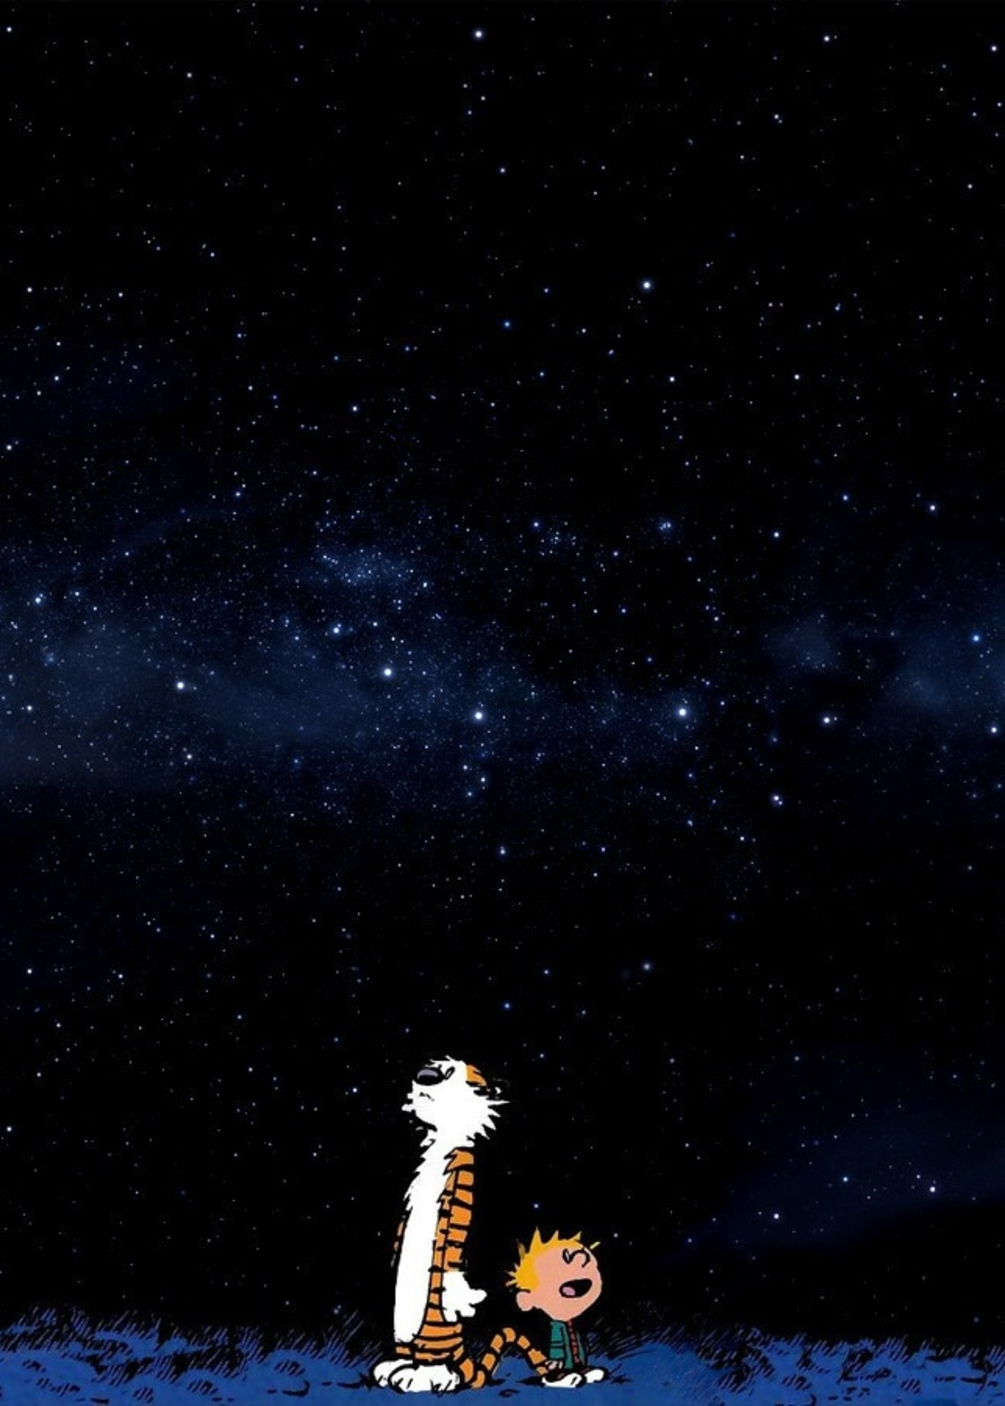
\includegraphics[height=\paperheight]{front_2}};
\node[titlestyle] (title) at ([yshift=5cm]current page.center) {\Huge\centering\bfseries\sffamily\parbox[c][][t]{0.95\paperwidth}{\centering Search for particles with anomalous charge in the IceCube detector\\[15pt]
{\huge Ward Van Driessche}}}; % Book title};
%\node[titlestyle] (super) at ([yshift=0cm]current page.center) {\Large\centering\bfseries\sffamily\parbox[c][][t]{0.95\paperwidth}{ Supervisor: prof. dr. D. Ryckbosch \\
%Dissertation submitted in fulfillment of the requirements for the degree of Doctor (Ph.D.) in Science: Physics}}; % Book title};
%\node[logostyle] (duper) at ([xshift=2.7cm,yshift=3.5cm]current page.south west)
%{\centering \bfseries\sffamily\parbox[c][][t]{0.4\paperwidth}{
\includegraphics[width=3cm]{logo_UGent_EN_RGB_2400_kleur_witbg.png}}};\node[substyle] (duper) at ([xshift=-4cm,yshift=3.5cm]current page.south east)
%{\bfseries\sffamily\parbox[c][][s]{0.37\paperwidth}{\begin{flushright}
%Department of Physics and Astronomy\\
%Faculty of Sciences\\
%Ghent University\\
%Academic year ???
%\end{flushright}}};
\end{tikzpicture}
\vfill
\endgroup
%----------------------------------------------------------------------------------------
%	Voorblad
%----------------------------------------------------------------------------------------
\pagenumbering{gobble}% Remove page numbers (and reset to 1)
\clearpage
\thispagestyle{empty}
~\vfill

\newpage
\vspace{5cm}
{\Huge \begin{center}
Search for particles with anomalous charge in the IceCube detector\\
\end{center}}
\vspace{1cm}
{\huge \begin{center}
Ward Van Driessche
\end{center} }
~\vfill

\noindent {\Large Auteur \dotfill
\begin{flushright}
\textcolor{red}{DATUM}
\end{flushright}}
\noindent {\Large Goedgekeurd door \dotfill
\begin{flushright}
prof. dr. Dirk Ryckbosch\\
Thesis Promotor
\end{flushright}}
\noindent {\Large Aanvaard door \dotfill
\begin{flushright}
prof. dr. Philippe Smet\\
Hoofd Examenjury\\
\end{flushright}}

\vspace{1cm}

\noindent {\Large Promotor: prof. dr. Dirk Ryckbosch \\
Co-promotor: prof. dr. Didar Dobur\\}
\vspace{2mm}

\noindent {\Large \begin{center}Proefschrift ingediend tot het verkrijgen van de academische graad van Doctor in de Wetenschappen: Fysica \end{center}}

\vspace{1cm}

\noindent{\Large Leden van de examenjury:\\}

\vspace{1mm}

\noindent{\Large Prof. dr. Philippe Smet, voorzitter (Universiteit Gent)\\
Prof. dr. Herwig Dejonghe  (Universiteit Gent)\\
Prof. dr. Nathalie Jachowicz (Universiteit Gent)\\
Prof. dr. Klaus Helbing (Bergische Universit\"at Wuppertal)\\
Prof. dr. Ioana Maris (Universit\'e libre de Bruxelles)
}

\vspace{1cm}

\noindent\begin{minipage}{0.7\textwidth}
~\vfill
{\Large Vakgroep Fysica en Sterrenkunde\\
Faculteit Wetenschappen\\
Universiteit Gent\\
Academiejaar 2018-2019}
\end{minipage}
\hfill%
\begin{minipage}{0.3\textwidth}
\begin{flushright}

\includegraphics[scale=10]{logo_UGent_EN_RGB_2400_kleur_witbg.png}

\end{flushright}\end{minipage}%
%----------------------------------------------------------------------------------------
%	Dankje
%----------------------------------------------------------------------------------------
\pagenumbering{gobble}% Remove page numbers (and reset to 1)
\clearpage
\thispagestyle{empty}
%\pagestyle{empty} % No headers

\begin{huge}
\textbf{Dankwoord - Acknowledgements}\\
\end{huge}
\begin{flushright}
\textit{All I can be is me - whoever that is $\sim$ Bob Dylan
\\}
\end{flushright}

\noindent Ondanks het maandenlang schrijven aan dit werk valt het me op hoe lastig het is om dit stukje op papier te zetten. Ik denk dat de meesten mij wel kennen als iemand die er de humor probeert in te houden, wat het niet evidenter maakt om een aantal mensen oprecht te bedanken. Ik kan tevens ook niet garanderen dat onderstaande tekst niet tot gefronste wenkbrauwen zal leiden. Ik blijf hoe dan ook de auteur van dit dankwoord.\\

\noindent Allereerst wilt ik natuurlijk mijn promotor professor Ryckbosch bedanken. Mijn eerste cursus deeltjesfysica is ondertussen al bijna acht jaar geleden en ik herinner mij hem nog maar vaag. Dat professor Ryckbosch mijn blik aanzienlijk verruimd heeft behoeft geen betoog. Ondanks het feit dat we niet meer in dezelfde gang zullen werken mogen, wat mij betreft, de niet-altijd-zo-serieuze-e-mails die zich sporadisch in mijn inbox bevonden zich blijven opstapelen. Dank u voor de voorbije jaren!\\

\noindent Thanks to the people from the BSM group for listening and helping in this work. Many thanks to Anna for all the times I had questions and for the abundunce of useful tips in how I could progress in my work. Thank you Frederik and Sarah for the nice times we had at the meetings. I'll come visit Wuppertal again at some point. I promise.\\

\noindent Merci, Antoine, pour ces dernières années durant lesquelles tu as voulu partager un bureau avec moi. Nous en avons vu beaucoup aller et venir, mais heureusement nos parcours se sont chevauchés suffisamment longtemps afin de me permettre un profond apprentissage du français. Bien sûr, ma copine a dû traduire ce petit mot parce que tu n'as jamais vraiment pris ton travail de professeur de français au sérieux. Je te souhaite encore beaucoup de succès dans ta carrière !\\

\noindent Aan alle anderen die ik de voorbije jaren collega's heb mogen noemen: bedankt voor de familiale sfeer die we op het INW mochten ervaren, de constante in- en uitstroom van mensen maakte dat er niet eenvoudiger op. Er zijn er zoveel waar ik de laatste jaren veel aan gehad heb, maar C\'eline, Ianthe en Giel: super bedankt voor de vele leuke gesprekken. Merci voor het nalezen, Stef, en nog veel succes de komende jaren.\\

\noindent Uiteraard hoor ik mijn familie en vooral mijn ouders te bedanken. Ik praat niet vaak over mijn werk in jullie bijzijn - vrije tijd is vrije tijd - dus ik wil jullie vooral bedanken om te luisteren naar al die andere onzin die uit mijn mond kwam tijdens onze etentjes en familiefeesten en om begrip te tonen toen ik voor de zoveelste keer zei dat we niet over mijn werk hoefden te babbelen. Jullie hebben mij misschien een beetje te vaak ``het is zo abstract dat het geen nut heeft om het te proberen uitleggen'' horen zeggen. Ik zal beter mijn best doen. Oh, en sorry voor mijn gedrag tijdens de examens. Die tijden zijn gelukkig voorbij.\\

\noindent De laatste jaren heb ik zoveel vrienden gemaakt dat ik bijna niet weet waar ik moet beginnen. Misschien hou ik mij het best bij diegenen waarvan iedereen weet dat ik ze niet uit mijn thesis kan houden. Dieter, Kris en Sam, er zijn nu al meer dan 16 jaar verstreken sinds het eerste middelbaar... Jullie weten ook dat het onmogelijk is om de goede dingen allemaal te beginnen opsommen. Ondanks het feit dat we elkaar al zo lang kennen, kijk ik uit naar de vele keren dat we nog zullen afspreken, hoe we nostalgisch gaan terugdenken en hoe we elkaars gedrag nog verder in het belachelijke gaan trekken.\\

\noindent James, mijn ventje, dit werk zou nooit volledig af zijn zonder de meest goedhartige persoon van het Waasland te vernoemen. Een beetje melig misschien, maar ik hoor je al snikkend lachen wanneer je voor het eerst zal lezen dat ik dit effectief heb neergepend. Dat je me nog veel goede raad mag geven en hopelijk vinden we beiden nog de tijd en goesting om te blijven fietsen.\\

\noindent Hannes, ik heb je fysiek zien opgroeien als 15-jarig snotneusje die toen al groter was dan ikzelf (ik zie je nog steeds in de nijlpaardkamer liggen toen je al 1m90 was en je je heup gebroken had). Mentaal mag je nog wat rijpen, maar ik ben alleszins al blij dat je mijn oor niet meer probeert te likken als we gaan fietsen. Er valt nog veel meer te zeggen, maar dat gaan we de lezers misschien best niet aandoen. Je bent er altijd voor me geweest en dat apprecieer ik nog meer dan ik soms doe uitschijnen.\\

\noindent Mijn klein Angeke, ik weet dat ik zei dat ik het leuk vond dat je veel babbelt toen we elkaar nog maar net kenden, maar zo had ik het me nu ook weer niet voorgesteld. Nee, schat, wat ben ik blij dat je het nog steeds met me uithoudt. Je bent er een groot deel van mijn doctoraat geweest en hebt me de nodige keren de duw in de rug kunnen geven. Mijn beste vriendin en mijn grootste liefde, team Wangeke doet dat goed en laat dit maar \'e\'en van de eerste stappen in ons hele lange verhaal worden.

~\vfill

\newpage

\pagenumbering{gobble}% Remove page numbers (and reset to 1)
\clearpage
\thispagestyle{empty}
\vspace*{\fill}
\textit{\\ \noindent If you can keep your head when all about you\\
\indent Are losing theirs and blaming it on you,\\
If you can trust yourself when all men doubt you,\\
\indent But make allowance for their doubting too;\\
If you can wait and not be tired by waiting,\\
\indent Or being lied about, don’t deal in lies,\\
Or being hated, don’t give way to hating,\\
\indent And yet don’t look too good, nor talk too wise:\\}
\textit{\\ \noindent If you can dream—and not make dreams your master;\\
\indent If you can think—and not make thoughts your aim;\\
If you can meet with Triumph and Disaster\\
\indent And treat those two impostors just the same;\\
If you can bear to hear the truth you’ve spoken\\
\indent Twisted by knaves to make a trap for fools,\\
Or watch the things you gave your life to, broken,\\
\indent And stoop and build ’em up with worn-out tools:\\}
\textit{\\ \noindent If you can make one heap of all your winnings\\
\indent And risk it on one turn of pitch-and-toss,\\
And lose, and start again at your beginnings\\
\indent And never breathe a word about your loss;\\
If you can force your heart and nerve and sinew\\
\indent To serve your turn long after they are gone,\\
And so hold on when there is nothing in you\\
\indent Except the Will which says to them: `Hold on!'\\}
\textit{\\ \noindent If you can talk with crowds and keep your virtue,\\
\indent Or walk with Kings - nor lose the common touch,\\
If neither foes nor loving friends can hurt you,\\
\indent If all men count with you, but none too much;\\
If you can fill the unforgiving minute\\
\indent With sixty seconds’ worth of distance run,\\
Yours is the Earth and everything that’s in it,\\
\indent And - which is more - you’ll be a Man, my son!\\ \\}
$\sim$ Rudyard Kipling

\vspace*{\fill}


%%%\pagenumbering{gobble}% Remove page numbers (and reset to 1)
\clearpage
\thispagestyle{empty}

\underline{\Huge{\sffamily Abstract}}\\
Bla bla bla
%Ik zou graag ook mezelf willen bedanken

%Of dat je in het middelbaar leert dat je eigenlijk een bundel bent van elektronen en protonen en bla bla bla, maar van zodra je fysica studeert besef je dat je eigenlijk een bundel trillingen in velden bent.


%Beautiful interplay of forces: i.e. strong force necessary to KEEP the neutrons as they are. Without it all neutrons would become protons! On the other hand; protons and neutrons would weigh the same if ....?

%Fun fact: entire lagrangian somewhere in a footnote?

%Leuk: bestaat ook niet zoiets als negatieve zwaartekracht. Nochtans wel alle andere flavors negatief en positief

%Waarom fysica? De vraag van Hiigs veld: als er een globaal minimum is kunnen we allemaal dood gaan. Ook zelfde filmpje
~\vfill


%----------------------------------------------------------------------------------------
%	TABLE OF CONTENTS
%----------------------------------------------------------------------------------------
\mainmatter

%\usechapterimagefalse % If you don't want to include a chapter image, use this to toggle images off - it can be enabled later with \usechapterimagetrue

\chapterimage{60seconds_StandardModelCube.jpg} % Table of contents heading image
\setcounter{page}{1}

\pagestyle{empty} % No headers

\renewcommand{\contentsname}{Table of Contents}
\tableofcontents % Print the table of contents itself

\cleardoublepage % Forces the first chapter to start on an odd page so it's on the right

\pagestyle{fancy} % Print headers again



%----------------------------------------------------------------------------------------
%	Nederlandstalige samenvatting
%----------------------------------------------------------------------------------------
\usechapterimagefalse
\chapterimage{whitepage.png} % whitepage voor samenvatting
\chapter*{Nederlandstalige Samenvatting}\label{nederlands}
\addcontentsline{toc}{chapter}{\protect\numberline{}Nederlandstalige samenvatting}%

\vspace{-5mm}
\textit{\begin{flushright}
Denkt aleer gij doende zijt en doende, denk dan nog $\sim$ Guido Gezelle
\end{flushright}}

\noindent De aanpak om nieuwe dingen te ontdekken binnen de fysica is de laatste eeuwen sterk ge\"evolueerd. De overgang van eenvoudige verklaringen naar theorie\"en die fenomenen niet alleen konden uitleggen, maar ook experimenteel konden reproduceren, bleek een cruciale stap naar een nieuwe methode in fysisch onderzoek. Als gevolg bracht deze methode nieuwe voorspellingen met zich mee; een theorie kon iets verklaren maar ook fenomenen beschrijven die tot dan toe nog niet werden geobserveerd. Deze fenomenen werden nadien ofwel waargenomen ofwel werd de theorie weerlegd. Hieruit volgde een natuurlijke evolutie in aanpak waarbij theorie en experiment elkaar horen te bevestigen.

In de loop van de 20ste eeuw viel er door de technologische ontwikkelingen veel te ontdekken. Men begon langzamerhand beter te begrijpen hoe de wereld in elkaar zit en hoe de wetten van de fysica neergeschreven konden worden. Wiskunde was daarin de taal van fysici om een theorie te ontwikkelen en experimenten te beschrijven. Experimentele deeltjesfysica kende zijn (eerste) hoogdagen in de jaren '60 waarbij deeltjesversnellers het ene na het andere nieuwe deeltje ontdekten: de ``particle zoo''. Fysici drongen aan op een theorie die een beter beeld kon geven; een handvol basisstenen (fundamentele deeltjes) en regels hoe deze deeltjes zich gedragen en hoe ze tot uiting komen. Die theorie werd de daaropvolgende jaren ontwikkeld en is gekend als het \textit{standaardmodel van de deeltjesfysica}. Het blijkt tot op heden een van de meest succesvolle ooit binnen het vakdomein van de fysica.\\

\noindent Met de ontdekking van het Brout-Engler-Higgs deeltje in 2012 werd de laatste bouwsteen, die door het standaardmodel voorspeld was, gevonden. Het model verklaart echter niet alles. We hebben bijvoorbeeld nog geen idee wat donkere materie precies is, waarom er zoveel minder antimaterie is in vergelijking met materie, enzovoort. Ook de schijnbaar wiskundige willekeur in het standaardmodel roept tot op heden nog steeds vragen op. Er lijken drie types leptonen te zijn. Waarom drie? En waarom zijn er welbepaalde symmetrie\"en die het standaardmodel beschrijven terwijl er ontelbaar veel andere symmetrie\"en mogelijk zijn? Waarom deze niet? Om deze redenen proberen fysici in experimenten op zoek te gaan naar processen die met de huidige, aanvaardde modellen nog niet beschreven kunnen worden. Dit zou ons een betere controle kunnen geven welk soort nieuwe theorie - waar er honderden van zijn - de juiste is. Deze experimenten worden steeds complexer: ze worden groter of miniteuzer en veelal een combinatie van beide. Deze complexiteit brengt een groter kostenplaatje met zich mee waardoor deze projecten goed beargumenteerbaar moeten zijn: ze zijn een gerichte tast in het duister.

Er zijn ook andere experimenten die met de waarnemingen van gekende deeltjes proberen om beter te achterhalen hoe bepaalde processen in ons universum tot stand komen. Een voorbeeld hiervan is het IceCube neutrino observatorium dat gesitueerd is in het ijs centraal op de Zuidpool. Het voornaamste doel van dit experiment is om gebruik te maken van neutrino's, deeltjes die zelden met materie interageren en net daarom een grote bron aan informatie bevatten omdat ze veel vertellen over hun oorsprong. We weten tot op heden nog maar weinig over de precieze werking van de bronnen van deze neutrino's.

Om zoveel mogelijk gebruik te maken van bestaande infrastructuur worden bestaande detectoren zoals IceCube ook gebruikt in zoektochten naar nieuwe fysica. Het doel van dit werk is om met behulp van het IceCube experiment na te gaan of er deeltjes bestaan met een electromagnetische lading die het standaardmodel niet voorspelt.\\

\noindent Het IceCube experiment werkt met behulp van lichtgevoelige modules die per 60 aan een kabel bevestigd zijn. 86 van zo'n kabels zijn verspreid in een hexagonaal vlak in het ijs dat in het totaal ongeveer een kubieke kilometer van volume inneemt. Geladen deeltjes zoals electronen en muonen die uit een neutrino-interactie kunnen komen, produceren licht in het ijs dat door deze modules waargenomen kan worden. Dit fenomeen is gekend als het Cherenkov-effect en zegt dat de hoeveelheid licht dat geproduceerd wordt afhangt van de lading van het deeltje. Aangezien de enige vrije deeltjes die we kennen een lading hebben die een veelvoud is van de elementaire lading van een elektron $e$, is het in theorie mogelijk om een onderscheid te maken tussen de gekende deeltjes en deeltjes met een lading die lager is dan $e$. Deze laatste maken geen deel uit van het standaardmodel en hun observatie zou een nieuwe start kunnen geven naar een meer omvattende theorie die mogelijks andere onopgeloste vragen helpt te verklaren.\\

\noindent De voornaamste uitdaging om op zoek te gaan naar dergelijke deeltjes blijkt de beperking van de detector zelf te zijn. Gekende deeltjes met een hele lage energie blijken niet eenvoudig te onderscheiden van deeltjes met een lage lading. Dit komt voornamelijk omdat de modules van de detector minimaal 17 meter van elkaar liggen. Hierdoor gaat veel van het licht verloren omdat het de optische instrumenten niet kan bereiken. In dit werk wordt er beschreven hoe deze nieuwe deeltjes onderscheiden kunnen worden van muonen en elektronen. Deze laatste ontstaan uit botsingen van kosmische straling met onze atmosfeer waar ze veelvuldig worden geproduceerd in zogenoemde ``air showers''. Ze kunnen ook de detector betreden als secundaire deeltjes nadat neutrino's interageren met het ijs. Deze neutrino's kunnen geproduceerd worden in kosmische processen zoals gamma ray bursts of supernova's, maar zijn er vooral in grote getale aanwezig door de voorgenoemde air showers.\\

\noindent De analyse beschrijft hoe er vanuit de IceCube data een selectie gemaakt kan worden om deze nieuwe fysica - als ze er is - zo goed mogelijk zichtbaar te maken. Na een reeks selecties om de kwaliteit van de data te verhogen, werden meerdere variabelen gebruikt en ontwikkeld om nadien ge\"implementeerd te worden in een ``Boosted Decision Tree'', i.e. een machine learning techniek die wordt gebruikt in datamining. Er werd tevens ook gebruik gemaakt van een resampling techniek genaamd ``pull-validation'' om de beperkte statistische mogelijkheden beter te handhaven. De enige mogelijke conclusie die getrokken kon worden was dat er geen indicatie was voor de aanwezigheid van deeltjes met een lage lading. Er werd een bovenlimiet opgesteld waarbij ook rekening gehouden werd met meerdere onzekerheden die deze limiet zouden kunnen be\"invloeden zoals de eigenschappen van het ijs waardoor het licht schijnt. Deze limieten zijn een verbetering van voorgaande experimenten en werden berekend volgens de techniek van Feldman en Cousins binnen een 90\% betrouwbaarheidsinterval.\\

\noindent Dit werk was een eerste poging om gebruik te maken van het IceCube experiment om op zoek te gaan naar nieuwe fysica in de vorm van deeltjes met een lading die tot op heden nog nooit zijn geobserveerd. Dergelijke deeltjes werden niet waargenomen waardoor een bovenlimiet werd opgesteld in de mate van hun aanwezigheid mochten ze weldegelijk bestaan.
\usechapterimagetrue

%----------------------------------------------------------------------------------------
%	INTRODUCTION
%----------------------------------------------------------------------------------------
\chapterimage{Header_Higgs_hunters_QandA.jpg} % Chapter heading image
\chapter*{Introduction}
\label{introduction}
\addcontentsline{toc}{chapter}{\protect\numberline{}Introduction}%

\textit{\begin{flushright} Scientists have become the bearers of the torch of discovery in our quest for knowledge $\sim$ Stephen Hawking
\end{flushright}}

\noindent Having a quest for knowledge seems to be a trait that belongs to human kind. The last couple of centuries there was a transition from providing simple explanations of physical phenomena to \textit{really understanding} the problem and properly describing it. More and more, a critical mindset became important in having new insights; being convinced of having the final answer is no longer enough. Theories are tested and are only accepted if they can be reproduced in experiments. This approach is not the most easy one and more than often, scientists encounter many obsticles along their way. However, I believe that the feeling scientists get when they have solved a puzzle and see their theory confirmed in an experiment is to be the driving force behind new discoveries and pushing the limits of current theories. Wanting to know what is beyond our current understanding has made us discover our planet (and others) and never stops us to come up with new questions.\\

\noindent Experimental particle physics is a field that tries to find the smallest detectable particles that make up matter and radiation. These particles carry certain properties such as mass, charge, spin, etc. and allow them to interact with each other. There are only a handful of fundamental interactions know to date: gravity, the strong force, the weak force and the electromagnetic force. It appears that nature follows certain physical rules that can be expressed in a mathematical form. Mathematics made it possible to write down our findings and to expand our knowledge. The theory that describes the last three of the four forces and classifies all known fundamental particles is called the Standard Model (SM) of particle physics. In Chapter \ref{ch:SM}, an overview is given of the properties of particles and interactions and ends with why fysicists think the SM in its current form cannot be the final answer.\\

\noindent There are many theories that try to expand the SM and are called ``Beyond-the-Standard-Model theories'' (BSM). They introduce new symmetries, new particles, new interactions, etc. Some of these theories also predict the existence of free particles with an electromagnetic charge that is lower than the electron charge, $e$. Quarks are known to have charges lower than $e$, but cannot exist freely. In Chapter \ref{ch:theoreticalmotivation} we motivate the possible existence of these particles and describe their assumed properties.\\

\noindent With the discovery of cosmic rays, a new field of physics was born: astroparticle physics. Experiments could be done on particles that could not originate from our solar system. The energy of these particles also has a wide range and offers to examine particles with a very high energy that do not have to be accelerated by man-made objects. For example, positrons, muons, pions, and kaons were first discovered in cosmic ray interactions. Cosmic rays play a crucial role in modern multimessenger astronomy along with gamma rays, gravitational waves and neutrinos. Each one of these fields has its strengths and weaknesses and many different experiments try to look for these respective signatures. Luckily, some of these experiments can also be used to look for BSM physics but have to account for the processes these experiments are designed to be sensitive too. Therefore, in Chapter \ref{ch:cr}, we give an overview of the physical processes that are visible in neutrino detectors. We will describe the origin of cosmic rays and neutrinos and how showers of particles are produced from cosmic ray interactions.\\

\noindent Charged particles can be detected by the production of Cherenkov radiation. These particles can be exotic particles, particles produced in cosmic air showers or secondaries that are created from neutrino interactions. The Cherenkov effect is explained in Chapter \ref{ch:cherenkov}, together with how charged particles lose their energy when traveling through matter.
To be able to detect high energetic neutrinos, it is crucial to make the instrumented volume of a detector as large as possible. In Chapter \ref{ch:icecube}, we describe how the IceCube Neutrino Observatory is constructed in the ice at South Pole. We describe the hardware components and how the ice is used and modeled for neutrino and charged particle detection.

The next part of this work has a larger focus on the technical details of this analysis that is dedicated to search for particles with an anomalous charge. The simulation steps are discussed in Chapter \ref{ch:simulation} and several analysis techniques that were used in this work are explained in Chapter \ref{ch:reconstruction}. In Chapter \ref{ch:space} an overview of the analysis is given and how it was possible to discriminate background events from events that originate from particles with an anomalous charge. We finalize with our findings if these particles exist or their maximal abundance that is measurable in the IceCube detector.

Chapter \ref{ch:summary} provides a summary and discussion of the work.

%------------------------------------------------

%----------------------------------------------------------------------------------------
%	PART
%----------------------------------------------------------------------------------------
%\part{Theory and Experiment}
%----------------------------------------------------------------------------------------
%	CHAPTER 1
%----------------------------------------------------------------------------------------
\chapterimage{StandardModel.jpg} % Chapter heading image
\chapter{The Standard Model of Particle Physics}
\label{ch:SM}
\begin{flushright}
\textit{\\A physicist is an atom's way of knowing about atoms $\sim$ George Wald\\}
\end{flushright}

\noindent The aim of this chapter is to give a summary of the framework that is used in particle physics.
This framework was developed in stages throughout the latter half of the 20th century and is known as the Standard Model of particle physics.
This model is a quantum field theory that is able to describe most of what is seen in particle physics experiments, and proved to be successful in predicting later experimental discoveries.
In this chapter, a brief historical overview of the development of this theory will be given together with a limited description in order to familiarize the reader with concepts that will be used throughout this work.
For a more in-depth and exhaustive discussion I refer to Refs. \cite{Povh,Peskin:1995ev,Agashe:2014kda,Bettini:2008zz}. We start with an overview of the constituent particles of the Standard Model, linking them to our everyday life. Secondly, a general description is given of the nature of forces. Thirdly, we go to a more mathematical and in-depth description of the Standard Model. Lastly, we present the many successes of this model and finish with an argumentation of why there is a need for physics beyond this model.

\section{What we call matter: fermions}
\label{sec:fermions}
Physics (from Ancient Greek: \gr φυσική \en - $physik\acute{\bar{e}}$, ``knowledge of nature'') is the natural science that studies matter.
Matter is made up of \textit{atoms} (from Greek: \gr ἄτομος \en - \textit{atomos}\footnote{Coined by ancient Greek philosophers Leucippus and his pupil Democritus who believed matter was made up of discrete units.}, ``indivisible'') that can bind together into molecules and account for what is around us in our everyday life.
Atoms are made up of a positively charged \textit{nucleus} that is surrounded by one or more \textit{electrons}. The nucleus and electrons are bound to each other via the electromagnetic force.
The nucleus is made up of one or more \textit{protons} and, typically, an approximately equal amount of \textit{neutrons}. Because of their similar characteristics, protons and neutrons are often referred to as \textit{nucleons} and together they make up more than 99.9\% of an atom's mass.
Nucleons are made up of smaller particles called \textit{quarks}\footnote{The word ``quark'' originally appeared in the novel \textit{Finnegans Wake} written by the Irish author James Joyce (1882–1941). The protagonist of the book dreams that he is serving beer to a drunken seagull. Instead of asking for ``three quarts for Mister Mark'' the inebriated bird says ``three quarks for Muster Mark''. Murray Gell-Man had the habbit of using names like ``squeak'' and ``squork'' for peculiar objects and after encountering the sentence in the book the name struck him as appropriate since the (then hypothetical) particle came in threes.}, which are, as far as we know, \textit{fundamental particles}. This means that we believe that there are no smaller substructures making up these objects and they are in essence mathematically best described as infinitely small.
Because of this, they are often referred to as pointlike.
In the Standard Model (SM), these particles are found to be \textit{fermions}, which have odd half-integer spins, obeying the laws of quantum mechanics.
The spin of a particle is often illustrated with its classical counterpart in which an object is spinning and thus carries an intrinsic angular momentum.
This analogy cannot be extrapolated to pointlike particles, but the property happens to hold the same units as the classical orbital momentum.
The spin of a particle seems to be just another property particles have, like charge or mass.
Fermions follow Fermi-Dirac statistics and therefore obey the Pauli exclusion principle. As a consequence, fermions cannot occupy the same place at the same time (more formally: no two fermions may be described by the same quantum numbers). This agrees with our macroscopic obeservations of matter in everyday life: matter interacts with matter; people cannot walk through walls!

In total, the SM distinguishes 24 different fermions that can be subdivided into two distinct classes: \textit{quarks} and \textit{leptons}. There are six quarks (up, down, charm, strange, top and bottom), and six leptons (electron, electron neutrino, muon, muon neutrino, tau and tau neutrino), along with the corresponding antiparticle for each of these fermions.
A summary of all the particles in the Standard Model is given in Figure \ref{SMparticles}.

\begin{figure}[t]
\centering
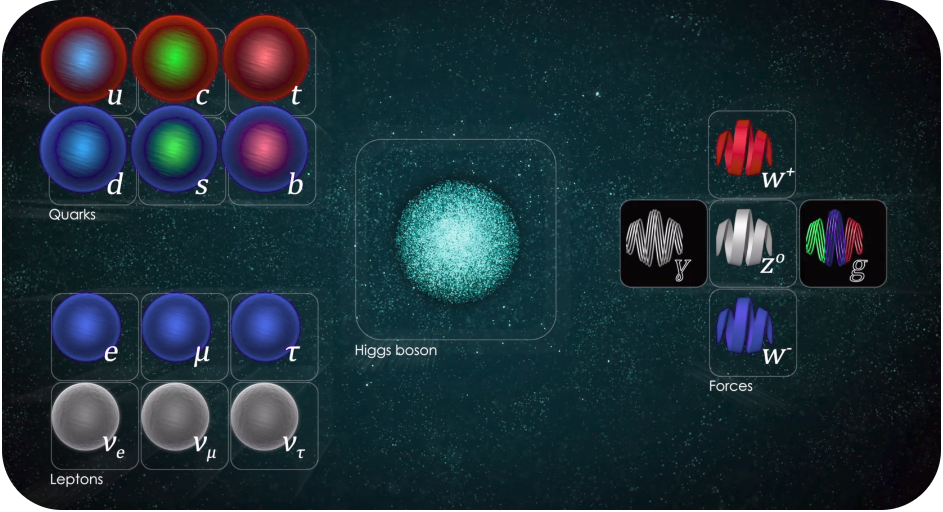
\includegraphics[width = \textwidth]{chapter1/img/SMparticles_rounded}
\caption{The Standard Model of particle physics distinguishes fermions (left) from bosons (right). The Brout-Englert-Higgs boson (middle) is more peculiar as it has no intrinsic spin and plays a special role in the theory. Charges for fermions are not explicitly written to account for antiparticles. Illustration from Ref. \cite{cernSMpic}.}
\label{SMparticles}
\end{figure}

\subsection{Leptons}
Leptons\footnote{\gr λεπτός \en (leptos) meaning thin, delicate, lightweight, or small. Originally, leptons were considered the ``light'' particles and hadrons the ``heavy'' particles, but the discovery of the tau lepton in 1975 broke that rule.} can be subdivided in two classes: electromagnetically charged particles ($e^-$, $\mu^-$ and $\tau^-$) and the neutral neutrinos\footnote{The Italian word for neutron (neutrone) sounds like the word neutral (neutro) with an augmentative suffix (-one) tacked on the end, making the word a little wordplay. In Italian, it sounds something like ``big neutral''. Replace the augmentative suffix -one with the diminutive suffix -ino and you have a ``little neutral'', which is a good description of what a neutrino is — a diminutive neutral particle.} ($\nu_{e}$, $\nu_{\mu}$ and $\nu_{\tau}$). Because of their charge, electrons are the well-known particles that combine together with nucleons into atoms. Being the lightest of the three charged leptons, the electron is said to be part of the first \textit{generation}, together with the electron neutrino. Muons differ only from electrons in mass\footnote{This characteristic is often referred to as \textit{lepton universality.}} and make up the second generation together with muon neutrinos. Similarly, tau particles and tau neutrinos define the third generation. All leptons have a corresponding antiparticle indicated by a positive charge (e.g. $e^+$) or a bar (e.g. $\bar{\nu}_e$). Neutrinos are proven to have a very small mass \cite{RevModPhys.88.030502} and interact only via the weak force (Section \ref{subsec:weak}), making them inherently very hard to detect.

\subsection{Quarks}
\label{sub:quarks}
The six quarks are called up, down, charm, strange, top and bottom quarks $((u,d),(c,s),(t,b))$.
Each generation is made up of a particle with charge +2/3 and one with -1/3 (also visualized in Figure \ref{SMparticles}). These charges are multiples of the absolute electron charge.
The difference between generations is again essentially the bare mass of the particles. Because quarks also interact through the strong force (see Section \ref{subsec:strong}), they combine into 
\textit{hadrons\footnote{\gr αδρός \en (adros) meaning thick, robust, massive, or large. This name alludes to the ability of the point-like quarks to bind together and form particles that are massive in a certain sense.}} (of which nucleons are the best known examples). Due to their color charge and the intrinsic behavior of the strong force, quarks cannot be observed freely: they always combine into color neutral particles, a property called \textit{confinement}. When a hadron, with its constituent quarks, is pulled apart, the attractive force between the quarks does not fall down rapidly since gluons carry color charge themselves. When these particles are pulled apart far enough, it becomes energetically more favorable to produce new quark-antiquark pairs, which again combine into color neutral particles\footnote{This process is called \textit{hadronization} and results into the production of ``jets'' in particle accelerators \cite{cmsjetsurl}.}. The energy requirement for the production of new particles is far below the one to separate the quarks far enough from each other to observe them separately. Antiquarks are again denoted with a bar (i.e. $\bar{u}$).

Because of their ability to interact via the strong force, particle accelerators in the 1960s led to the discovery of a plethora of possible quark combinations, something that is often referred to as the ``particle zoo''.



\section{How particles communicate: interactions}

There are four fundamental interactions known to exist: \underline{gravity} and \underline{electromagnetism}, which produce significant long-range forces, and the \underline{strong} and \underline{weak forces} that only express themselves at (sub)atomic distances and govern nuclear interactions. These are explained in more detail below and an overview is given in Table \ref{tab:forces}.

Particles interact with each other through the exchange of \textit{gauge bosons} or \textit{force carriers}\footnote{A classic and very simplistic way of looking at force carriers is to imagine two people standing on a boat. The force carrier is a heavy ball that can be thrown from one person to the other. Doing so, both persons will move in opposite direction.}. Gauge bosons are bundles of energy, \textit{quanta}, and can be seen as excitations of one of the force fields.

Fields are a mathematical approach used by physicists to describe what we observe in experiments. Although the use of fields is very natural, the concept might feel a bit unfamiliar. In the following, the known forces are described in more detail. Gravity plays less of a role in subatomic physics, but is added for completeness and is mainly used to make the reader more familiar with the concept of a field.

\begin{table}[]
\centering
%\begin{footnotesize}
\caption{Summary of the known forces and their properties. The relative strengths are quoted in terms of a dimensionless coupling constant ($\alpha_g, \alpha_w, \alpha$ and $\alpha_s$). These ``constants'' actually depend on the energy. These number were obtained from Ref. \cite{hyperphysicsStrengths}.}
%Ref: https://web.archive.org/web/20160304133522/https://www.pha.jhu.edu/~dfehling/particle.gif. A nice webpage explaining... :https://profmattstrassler.com/articles-and-posts/particle-physics-basics/the-known-forces-of-nature/the-strength-of-the-known-forces/
%http://web.mit.edu/sahughes/www/8.022/lec01.pdf}
\label{tab:forces}
\resizebox{\textwidth}{!}{%
\begin{tabular}{|l |c|c|c|c|}
\hline
\cellcolor[HTML]{F1A91E} & \cellcolor[HTML]{F1A91E}                              & \cellcolor[HTML]{F1A91E}\textbf{Weak} & \cellcolor[HTML]{F1A91E}\textbf{Electromagnetic} & \cellcolor[HTML]{F1A91E}\\ 
\multirow{-2}{*}{\cellcolor[HTML]{F1A91E}\textbf{Interaction}} & \multirow{-2}{*}{\cellcolor[HTML]{F1A91E}\textbf{Gravitational}} & \multicolumn{2}{c|}{\cellcolor[HTML]{F1A91E}\textbf{Electroweak}}               &      \multirow{-2}{*}{\cellcolor[HTML]{F1A91E}\textbf{Strong}}                \\ \hline
\textbf{Acts on} &mass/energy  & weak flavor  & electric charge & color charge  \\ \hline
\textbf{Couples to}  & all particles & all fermions   & electrically charged particles & quarks, gluons \\ \hline
\textbf{Mediation}                                 & not yet observed                                      & $W^+, W^-,Z$                 & $\gamma$                                & gluons \\ \hline
\textbf{Rel. strength} & $10^{-39}$ & $10^{-6}$ & 1/137 & 1 \\ \hline
%Long-distance                              & $\frac{1}{r^2}$                                        & $\frac{1}{r}e^{-m_{W,Z}\cdot r}$   & $\frac{1}{r^2}$                          & \multicolumn{2}{c|}{$r$} \\ \hline
\end{tabular}%
}
%\end{footnotesize}
\end{table}

\subsection{Gravity}
Gravity (from Latin/old French: gravitas/grave, ``weighty, heavy'') is the phenomenon wherein massive objects are attracted to each other. Gravitation is famously described by the theory of general relativity proposed by Einstein in 1915. Compared to the other forces, gravity is intrinsically very weak\footnote{Two magnets that fit in the palm of your hand can deliver a force which is of similar strength as the force that our entire planet exerts on a human body.} and is not described in the SM (see Section \ref{sec:sm}). This is why gravity is often left out in discussions of particle physics experiments, but is crucial for understanding astronomical objects and how they influence each other. It can, however, be used to explain the concept of a field in a very natural way.

A very good description of gravitation was already provided centuries ago. First published on July 5th, 1686 was Newton's work \textit{Philosophiae Naturalis Principia Mathematica} (``the Principia'') that first introduced several formulas that are still widely used today. The equation of the force exerted by two massive bodies takes the following form,
\begin{equation}
F = G \frac{m_1 m_2}{r^2},
\end{equation}
where $F$ is the gravitational force acting between two objects, $m_1$ and $m_2$ are the masses of the objects, $r$ is the distance between their center of mass, and $G$ is the gravitational constant.

Newton's law states that two massive bodies will exert a force on one another that is proportional to their masses, but inversely proportional to the square of the distance between them. Newton realized this would mean that at any given instant in time all massive objects in the universe would know from every other object in the universe where it is located and how massive it is\footnote{Imagine the attraction of the Moon to the Earth: how are both ``communicating''?}. Because of this, Newton himself believed his explanation could not be the final answer. The answer is fully described in Einstein's work of general relativity, but the first idea in the right direction was introduced by Laplace in 1783. Laplace explained that massive objects do not ``feel'' each other but distort space and time in such a way that objects that are attracted, ``fall'' towards each other. Field theory makes it possible to treat the laws of physics as a local property instead of an action from a distance.


To date, it has not been possible to describe gravity in the framework of quantum field theory like the other fundamental forces, although, there is still much ongoing work. The gauge bosons from such a quantum field theory for gravity are mostly referred to as \textit{gravitons}.

\subsection{Electromagnetism}
The electromagnetic field (from Ancient Greek: \gr ἤλεκτρον \en $\bar{e}lektron$, ``amber'', and \gr μαγνῆτις λίθος, \en \textit{magnetis lithos}, which means ``Magnesian stone''\footnote{In 1641, Kircher described the magnetic properties of the Magnesian stone in his book \textit{Magne sive de arte magnetica opus tripartitum} \cite{kircher1641athanasii}.}) presents itself in the electrical and magnetical forces. In the late 1870s, the publication of Maxwell's \textit{A Treatise on Electricity and Magnetism} showed that the electric and magnetic interactions of negative and positive charges are mediated by one force: electromagnetism. Particles carrying a charge of one of these forces can attract or repel each other.

Similar to the gravitational field, the electromagnetic field pervades all around us, providing the necessary description of how charged particles interact with each other. The interaction of nuclei, which have a positive electric charge, and electrons makes up most of what is described in chemistry. 

The force carrier of electromagnetism is called a \textit{photon}, or in other words: light.
\subsection{Weak force}
\label{subsec:weak}
The weak force is one aspect of the overarching electroweak theory that combines electromagnetism and the weak force. As opposed to gravity and electromagnetism, it only takes place at very small subatomic distances\footnote{The reason being is that the force carriers are massive; more info in Section \ref{sec:sm}.}. One well known phenomenon that is governed by the weak force is \textit{beta decay} in which free neutrons decay into protons and produce an extra electron and antielectron neutrino. Another beautiful example of the weak force is the driving mechanism in the Sun's thermonuclear process that makes it shine. This process cannot be explained by chemical processes but with the fusion of hydrogen cores into helium where two out of four protons are converted to neutrons. This conversion of the proton into a neutron is explained by the weak force.

The force carriers of the weak force are the $W^+$, $W^-$ and $Z$ bosons. 
Quantum field theory tells us that the interaction strength of particles depends on the coupling constants and the properties of the mediator particles. The coupling constants of the weak force are of similar magnitude as those in electromagnetism. However, because of the mass of the weak force carriers, the interaction strength at low energies, such as radioactive decay, becomes much smaller\footnote{The mediator term for photons scales with $\frac{1}{q^2}$ with  $q$ the momentum of the mediator. $W$ and $Z$ boson mediator terms scale with $\frac{1}{q^2 - M^2}$ with $M$ the mass of the mediator. When $q$ is low, for example in radioactive decays, this term becomes very small due to the mass of the bosons. On the other hand, if $q$ and $M$ are of similar magnitude, the weak force is strong. For example, the top quark decay will most likely happen via the weak force.}. This makes the force seem weak, hence the name\footnote{It was Fermi who first came up with a proper description of the beta decay in 1933. However, he described the interaction as a 4-point interaction, making it only valid up to energies below 100 GeV.}.\\

\noindent The weak force also has some peculiar properties that are unique in a number of respects:

\vspace{2mm}
\begin{itemize}
\item it is the only interaction that violates parity symmetry and even does so maximally (V-A interaction),
\item its force carriers are massive as opposed to all other force carriers,
\item it is the only force capable of changing quarks from one family into a quark of another family.
\end{itemize}

\subsection{Strong force}
\label{subsec:strong}
As indicated in Section \ref{sec:fermions}, nuclei are made up of protons and neutrons. However, up to now the forces described in this section cannot explain how they can make up a stable combination. The positive/neutral electromagnetic charge of the protons/neutrons would even suggest the opposite. Protons and neutrons are made up by quarks that carry a quantity called \textit{color charge}. Particles carrying a color charge participate in interactions of the strong force. Due to the principle of \textit{self interaction}, the strong force only manifests itself on very small scales\footnote{As opposed to the weak force where the short distance behaviour is explained due to the mass of the force carriers.}.

The force carriers of the strong force are called \textit{gluons}. These gluons carry a color charge themselves and are massless.

Aside from holding nucleons together, the strong force is also responsible for around 99\% of the mass of the nucleon's mass. The massless gluons have a \textit{quantum chomodynamics binding energy} so large that it makes up the bulk of the mass via Einstein's $E=mc^2$ relation. Only a small percentage of the total nucleon mass comes from the bare quark masses.

\subsection{A note about bosons}
As opposed to fermions, which obey Fermi-Dirac statistics and cannot occupy the same quantum state, bosons follow Bose-Einstein statistics\footnote{The name ``boson'' originates from Dirac who wanted to commemorate the contributions of Indian physicist S.N. Bose who, together with Einstein, theorized the characteristics of elementary particles that follow Bose-Einstein statistics \cite{farmelo2009strangest}.}. Bosons carry integer spins ($s=0,1,2,$ etc.) while fermions carry half-integer spins ($s=1/2,3/2,$ etc.). As a result, bosons have no problem occupying the same place at the same time (more formally: two or more bosons may be described by the same quantum numbers). As an example, lasers are very powerful tools that make large numbers of photons to have almost exactly the same energy (which is expressed in having the same color) and direction. Fermions, on the other hand, cannot share the same quantum number, e.g. electrons cannot have the same orbit in an atom. If electrons were bosons, chemistry and matter all around us would be nothing like we see today.

\section{The Standard Model in theory}
\label{sec:sm}
Most of the text below is based on the very elaborate book from Franz Mandl and Graham Shaw, \textit{Quantum Field Theory} \cite{mandl2013quantum}.\\
\\
The Standard Model is a \textit{quantum field theory}, meaning its fundamental objects are fields of a quantum nature that are defined at all points in spacetime. These fields are
\vspace{2mm}
\begin{itemize}
\item fermion fields, $\psi$, which describe ``matter particles'';
\item electroweak boson fields, $W^1, W^2, W^3$ and $B$;
\item gluon fields, $G^a$; and
\item the Higgs field, $\phi$.
\end{itemize}

\vspace{2mm}

\noindent Quantum field theory treats particles as excited states of one of these underlying fields, so called \textit{field quanta}. The difference between classical and quantum fields is that they are operator-valued. Classical fields can in principle take on distinct values at each point in space whereas a quantum field accomodates observations of quantum mechanics such as
\vspace{2mm}
\begin{itemize}
\item objects have characteristics of both particles and waves (called ``wave-particle duality'');
\item the quantization of energy, meaning that only discrete energy values are possible;
\item the lowest achievable energy is not equal to absolute zero, but has a zero-point energy\footnote{The zero-point energy follows from the Heisenberg uncertainty principle that states that the position and momentum of a particle are not fixed but have a small range of variance: $\sigma_x\sigma_p \geq \frac{\hbar }{2}$. A system having zero energy would imply a motionless system at a fixed location, violating the uncertainty principle and is therefore forbidden.}.
\end{itemize}

\vspace{2mm}

\noindent The dynamics of the quantum state and the fundamental fields are determined by the Lagrangian density $\mathcal{L}$. Writing the time and space coordinates in the form $(t,\mathbf{x}) = (x^0, x^1, x^2, x^3) = x^\mu$, the equations of motion of these fields can be written as:
\begin{equation}
\frac{\partial}{\partial x_{\mu}}\left[\frac{\partial \mathcal{L}}{\partial\left(\partial\phi/\partial x^{\mu}\right)}\right] - \frac{\partial \mathcal{L}}{\partial \phi} = 0,
\end{equation}
which follow from the principle of least action. The Lagrangian function depends on the fields and how these fields change in spacetime: $\mathcal{L(\phi,\nabla\phi)}$. Quantization of these fields can be obtained by interpreting the coordinates and momenta as Heisenberg operators, and subjecting these to canonical commutation relations. 

Furthermore, the Standard Model is a gauge theory in which the Lagrangian is invariant under certain Lie groups (referred to as the symmetry group or the gauge group of the theory) of local transformations. For quantized gauge groups, the quanta of the gauge fields are referred to as \textit{gauge bosons}. A gauge theory is a mathematical model that has a gauge freedom; there are mathematical degrees of freedom that are redundant. In other words: different mathematical expressions describe the exact same physical system and are in that sense not physical. An experiment could never uniquely determine their values, even in principle\footnote{Imagine a perfect cylinder that can be twisted without deforming. It is not possible to distinguish a cylinder that has been twisted or not. To be able to determine it, an initial gauge has to be present. A horizontal line drawn on the cylinder can determine if the cyclinder has been deformed or not.}. If the phase of the wavefunction is changed by a different amount at each point in spacetime and the physics remains unchanged, the Lagrangian is said to follow a \textit{local gauge symmetry}\footnote{See Ref. \cite{mandl2013quantum}.}.

The Standard Model is defined by the local SU(3) $\times$ SU(2) $\times$ U(1) gauge symmetry. Each element gives rise to one of the three fundamental forces.
\subsection{SU(3): quantum chromodynamics}
\label{subsec:QCD}
The quantum chromodynamics (QCD) sector defines the interactions between quarks and gluons. Since leptons do not carry color charge, they do not participate in this interaction. The Dirac Lagrangian of the quarks coupled to the gluon fields is given by


\begin{equation}
\mathcal{L}_{QCD} = \sum_{\psi} \bar{\psi_i} \left(i \gamma^\mu \left(\partial_\mu  \delta_{ij} - i g_s G^a_{\mu} T^a_{ij}\right) - m_\psi \delta_{ij} \right) \psi_j - \frac{1}{4} G^a_{\mu\nu}G^{\mu\nu}_a,
\end{equation}

where we sum over the fields of the strong charge and\\
\indent $\psi_i$ is the Dirac spinor of the quark field (the subscript $i={r,g,b}$ represents the color charges);\\
\indent $\gamma^\mu$ are the Dirac matrices;\\
\indent $G^a_\mu$ is the 8-component $\left(a=1,2,...,8\right)$ SU(3) gauge field;\\
\indent $T^a_{ij}$ are the $3\times3$ Gell-Mann matrices (generators of the SU(3) color group);\\
\indent $G^a_{\mu\nu}$ are the field strength tensors for the gluons;\\
\indent $g_s$ is the strong coupling constant;\\
\indent $m_\psi$ corresponds to the quark masses.

\subsection{SU(2) $\times$ U(1): electroweak}
\label{subsec:ew}
The electroweak (EW) sector is a Yang-Mills gauge theory with the symmetry group SU(2)$_L$ $\times$ U(1). The Lagrangian is given by

\begin{equation}
\label{eq:EW}
\begin{split}
\mathcal{L}_{EW} &= \sum_{\psi} \bar{\psi} \gamma^\mu \left(i\partial_\mu -  \frac{g'}{2}Y_W B_\mu - \frac{g}{2} \overrightarrow{\tau_L} \overrightarrow{W}_\mu \right) \psi - \frac{1}{4} W^{\mu\nu}_a W^{a}_{\mu\nu} -\frac{1}{4} B^{\mu\nu} B_{\mu\nu} \\ 
&= \bar{Q}_i i D_\mu \gamma^\mu Q_i + \bar{u}_i i D_\mu \gamma^\mu u_i + \bar{d}_i i D_\mu \gamma^\mu d_i + \bar{L}_i\left(iD_\mu\gamma^\mu\right)L_i + \bar{l}_{R,i}\left(iD_\mu\gamma^\mu\right)l_{R,i} \\ &
- \frac{1}{4} W^{\mu\nu}_a W^{a}_{\mu\nu} -\frac{1}{4} B^{\mu\nu} B_{\mu\nu},
\end{split}
\end{equation}
where\\
\indent $B_\mu$ is the U(1) gauge field;\\
\indent $Y_W$ is the weak hypercharge\footnote{The weak hypercharge follows the relation $Y_W = 2\left(Q-T_3\right)$ where $Q$ is the electric charge and $T_W$ the third component of the weak isospin.} (the generator of the U(1) group);\\
\indent $\overrightarrow{W}_\mu$ is the 3-component SU(2) gauge field;\\
\indent $\overrightarrow{\tau_L}$ are the Pauli matrices (infinitesimal generators of the SU(2) group with subscript $L$ to indicate that they only act on left-chiral fermions);\\
\indent $g'$ (weak hypercharge) and $g$ (weak isospin) are the U(1) and SU(2) coupling constants respectively;\\
\indent $W^{a\mu\nu} (a=1,2,3)$ and $B^{\mu\nu}$ are the field strength tensors for the weak isospin and weak hypercharge fields;\\
\indent $Q, u$ and $d$ are the left-handed doublet, right-handed singlet up and right-handed singlet down quark fields;\\
\indent $L$ and $l$ are the left-handed doublet and right-handed singlet lepton fields.\newline
\\
\noindent The field strengths are given by
\begin{equation*}
\begin{split}
W^a_{\mu\nu} &= \partial_\mu W^a_\nu - \partial_\nu W^a_\mu + g \epsilon^{abc}W^b_\mu W^c_\nu,\\
B_{\mu\nu} &= \partial_\mu B_\nu - \partial_\nu B_\mu,
\end{split}
\end{equation*}
\noindent and the covariant derivative for the left- and right-handed fermions by,

\begin{equation*}
\begin{split}
D_\mu \psi_L &= \left(\partial_\mu - i\frac{g}{2} \tau_a W^a_\mu - i \frac{g'}{2} Y_W B_\mu \right) \psi_L, \\
D_\mu \psi_R &= \left(\partial_\mu - i\frac{g'}{2} Y_W  B_\mu\right)\psi_R,
\end{split}
\end{equation*}
\noindent where one simply has to fill in the appropriate weak hypercharge for the corresponding quark and lepton fields.


It is worth noting that no terms are included for fermion masses. These would have the form of $m\bar{\psi}\psi$ but are forbidden as they would break the SU(2)$_L$ $\times$ U(1) gauge invariance. Neither is it possible to add explicit mass terms for the U(1) and SU(2) gauge fields. 
\subsection{Brout-Englert-Higgs mechanism}
\label{subsec:BEH}
To come to a viable description of the elementary particles, one is required to introduce masses into a chiral theory. The masses of the $W$ and $Z$ bosons are explained by use of the Brout-Englert-Higgs (BEH) mechanism formulation. Introducing one or more scalar fields, the Higgs fields, which can acquire a vacuum expectation value (vev), make it possible to spontaneously break a symmetry in the Lagrangian. We say that electroweak symmetry is broken down to a weak symmetry and electromagnetism. 
%According to the Goldstone theorem, every spontaneously broken continuous symmetry results in a massless scalar particle: the Goldstone boson. Hence, the number of Goldstone bosons in a theory is equal to the number of broken generators of the symmetry group.

Since the electroweak theory after symmetry breaking should contain three massive gauge bosons ($W^+, W^-$ and $Z$), the scalar fields of the Higgs fields should contain at least three degrees of freedom. The simplest approach to do this is by introducing a complex, scalar SU(2) doublet $\Phi$ with positive hypercharge $\left(Y_W=1\right)$,
\begin{equation}
\label{eq:higgsdoublet}
\Phi = \begin{pmatrix} \phi^+ \\ \phi^0 \end{pmatrix} = \frac{1}{\sqrt{2}} \begin{pmatrix} \phi_1 + i\phi_2 \\ \phi_3 + i\phi_4 \end{pmatrix},
\end{equation}
Similar to the SU(2) symmetry of the EW theory, four new gauge particles are introduced: $H^+, H^-, H^0$ and $H$.


\paragraph{Massive bosons}
Having introduced this scalar doublet, one needs to add the corresponding Lagrangian term to the electroweak Lagrangian from Eq. \ref{eq:EW}, 

\begin{equation}
\label{eq:higgslagrangian}
\mathcal{L}_S = \left(D^\mu\Phi\right)^\dagger \left(D_\mu \Phi\right) - V\left(\Phi\right), \ \ \textrm{with } V\left(\Phi\right) = \mu^2 \Phi^\dagger\Phi + \lambda \left(\Phi^\dagger \Phi\right)^2. 
\end{equation}
\noindent The first term is the kinetic term while the second corresponds to the potential of the scalar field\footnote{The form of the potential is not known from first principles, but is the simplest form that can explain the spontaneous symmetry breaking mechanism.}. The linear term in the potential needs to be positive to ensure an absolute minimum in the Lagrangian. The quadratic term can either be positive or negative, depending on whether $\mu^2 > 0$ or $\mu^2 < 0$. This is illustrated in Figure \ref{fig:BEHpotential}. In the former case, the scalar potential has an absolute minimum at the origin:

\begin{figure}
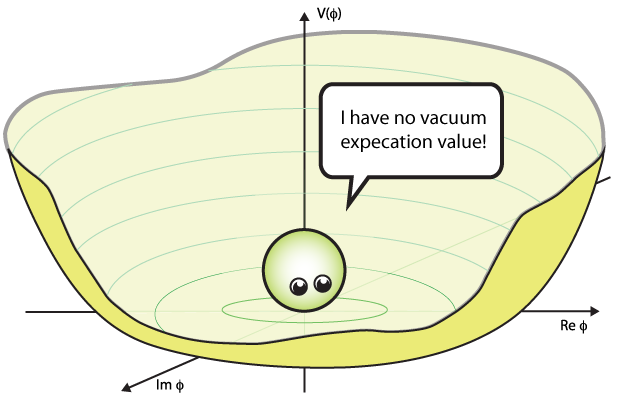
\includegraphics[width=0.5\textwidth]{chapter1/img/BoringPotential}
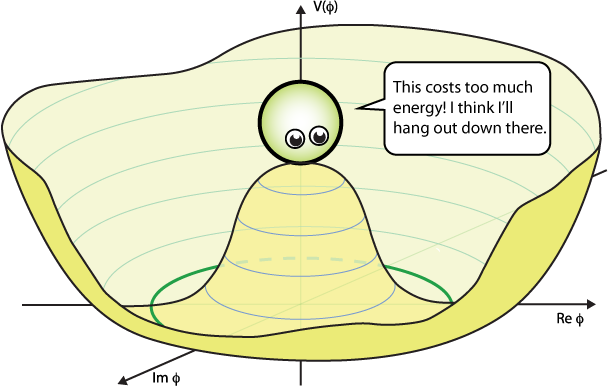
\includegraphics[width=0.5\textwidth]{chapter1/img/Higgs-Potential-lookdown}
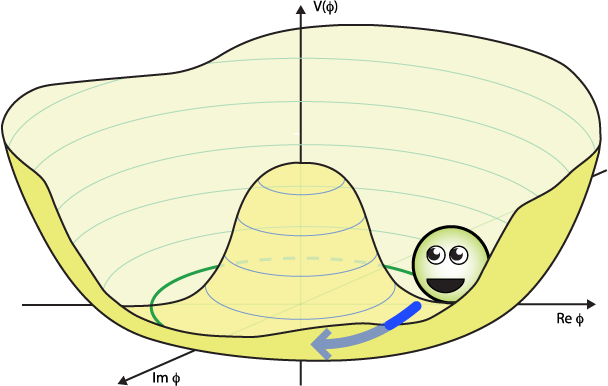
\includegraphics[width=0.5\textwidth]{chapter1/img/Higgs-Potential-Goldstone}
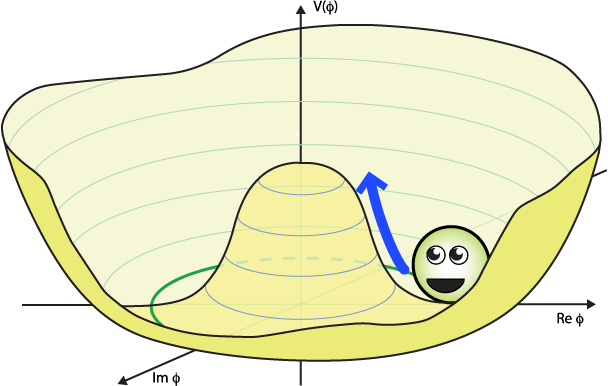
\includegraphics[width=0.5\textwidth]{chapter1/img/Higgs-Potential-radial}
\caption{In this example the Higgs potential is illustrated in function of a complex scalar field (2D). The principle is the same for a complex scalar doublet but a lot harder to visualize. \textit{Top left:} the Higgs potential with $\mu^2 > 0$, there is no vacuum expectation value. \textit{Top right:} $\mu^2 < 0$, the origin is now a maximum and not stable; the scalar field will move to the lowest possible energy state. \textit{Bottom left:} a flat direction in the potential corresponds to a massless Goldstone mode (remember there are two extra scalar fields in the full theory, meaning there are a total of three). \textit{Bottom right:} the concave shape of the potential near the minimum defines the Higgs boson mass. Illustrations from Ref. \cite{flip}.}
\label{fig:BEHpotential}
\end{figure}


\begin{equation}
\label{eq:zerominimum}
\langle 0|\Phi|0\rangle \equiv \Phi_0 = \begin{pmatrix} 0 \\ 0 \end{pmatrix}.
\end{equation} 
From Eq. \ref{eq:higgslagrangian} and \ref{eq:zerominimum}, one can see that the kinetic term does not give rise to massive particles in this scenario\footnote{Easy to see when substituting $v=0$ in Eq. \ref{eq:massesHiggs}.}. In the case of $\mu^2 < 0$, the minimum is no longer located at the origin of the fields: $\partial_{|\Phi|} V(|\Phi|) = 0$ for $|\Phi| = \sqrt{-\frac{\mu^2}{2\lambda}}$, hence one possible solution is\footnote{It is not possible for the charged part of the fields to have a vacuum expectation value as this would not be in agreement with electromagnetism. The upper part in Eq. \ref{eq:vev2} is therefore set to zero.}
\begin{equation}
\label{eq:vev2}
\langle 0|\Phi|0\rangle \equiv \Phi_0 = \begin{pmatrix} 0 \\ \frac{v}{\sqrt{2}} \end{pmatrix}, \ \ \textrm{with} \ \ v = \sqrt{-\frac{\mu^2}{\lambda}}.
\end{equation} 
$v$ is referred to as the \textit{vacuum expectation value} to reflect that the Higgs field is always ``on''. To investigate the terms, we can expand the field around the minimum:

\begin{equation}
\Phi(x) = \begin{pmatrix} \theta_2(x) + i\theta_1(x) \\ \frac{v+H(x)}{\sqrt{2}} - i\theta_3(x) \end{pmatrix} = e^{i\theta_a\tau_a}\begin{pmatrix} 0 \\ \frac{v+H(x)}{\sqrt{2}} \end{pmatrix}.
\end{equation}
Implementing this into Eq. \ref{eq:higgslagrangian} would yield the existence of unphysical fields $\phi_{1,2,3}$ that give rise to three extra degrees of freedom that were not present in the original Lagrangian\footnote{In Eq. \ref{eq:higgslagrangian}, the vector fields are massless and each give rise to 2 d.o.f. The vev makes the three vector fields massive, thus adding 3 d.o.f.\textit{and} introduce three unphysical fields.}. Since a change of variables cannot alter the number of d.o.f. of a system, one can conclude that three fields do not represent physical fields. They can be removed by fixing a gauge, the unitary gauge, that breaks the original symmetry of the system.
\begin{equation}
\label{eq:vev}
\Phi(x) \rightarrow e^{-i\theta_a\tau_a}\Phi(x) = \begin{pmatrix} 0 \\ \frac{v+H(x)}{\sqrt{2}} \end{pmatrix},
\end{equation}
where we have introduced a new scalar field $H(x)$. After inserting this in the kinetic part of the scalar Lagrangian (Eq. \ref{eq:higgslagrangian}) and redefining the gauge fields as

\begin{equation}
\begin{split}
W^\pm_\mu &= \frac{1}{\sqrt{2}}\left(W^1_\mu \mp iW^2_\mu\right),\\
Z_\mu &= \frac{1}{\sqrt{g^2 + g'^2}}\left(gW^3_\mu - g'B_\mu\right),\\
A_\mu &= \frac{1}{\sqrt{g^2 + g'^2}}\left(gW^3_\mu + g'B_\mu\right),
\end{split}
\end{equation}
we find for the kinetic part of the scalar Lagrangian:

\begin{equation}
|D_\mu\Phi|^2 = \frac{1}{2} \left(\partial_\mu H\right)^2 + \frac{1}{2}g^2\left(v+H\right)^2W^+_\mu W^{-\mu} + \frac{1}{8}\left(v+H\right)^2 \left(g^2 + g'^2\right)Z_\mu Z^\mu.
\end{equation}
Since mass terms enter this equation in the general form of $M^2_W W_\mu W^\mu$ for the $W$ bosons and $\frac{1}{2}M_Z^2 Z_\mu Z^\mu$ for the $Z$ boson, the mass terms of the gauge bosons after spontaneous symmetry breaking can be written down as:

\begin{equation}
\label{eq:massesHiggs}
\begin{split}
M_W &= \frac{1}{2}vg,\\
M_Z &= \frac{1}{2}v\sqrt{g^2+g'^2},\\
M_A &= 0,\\
\end{split}
\end{equation}
where it is clear that the photon remains massless\footnote{Because the $W$ and $Z$ bosons are massive, it costs energy to produce them and so the weak force is only really effective over a short distance. This is in contrast to the massless photons that result into a long range electomagnetic force. Thus, the Higgs field is responsible for the ``weakness'' of the weak force.}.\\


%\begin{corollary}[Eating the gauge bosons]
%A vev can give rise to massless Goldstone bosons. These particles correspond to the infinite possibilities of its phase in the potential. However, this would also lead to extra degrees of freedom in the Lagrangian. Therefore, one has to fix a gauge that results in the disappearance of the bosons and making the vector bosons of the original fields massive. 

%Specifically, the two massless $W^1, W^2$ bosons in the electroweak theory ($2 \times 2$ polarizations\footnote{A massless particle cannot have a third polarization, similar to a photon: it is traveling at the speed of light so it cannot have a polarization in the direction of propagation, only longitudinal.} = 4 d.o.f.) and two charged Higgses (2 d.o.f.) sum to a total of six degrees of freedom. In the broken theory, we have two massive $W^+,W^-$ bosons ($2 \times 3$ polarizations), which again total to six degrees of freedom.

%Similarly, the $W^3, B$ ($2\times2$ d.o.f.) and $H^0$ (2 d.o.f.) combine into the neutral $Z$ (massive, 3 d.o.f.), the $\gamma$ (2 d.o.f.) and the scalar $H$ (1 d.o.f.).

%Similar to the nucleons having a mass that is much greater than the summed mass of its constituents, the Higgs fields gives rise to the mass of these gauge bosons. In the case of nucleons, it is primarily the potential energy of the strong force that is responsible for the total mass following $E=mc^2$. The coupling of the gauge bosons to the Higgs field gives a sense of inertia to the particle. The particle does not float freely in vacuum but interacts with the ever present Higgs field (with a vev $\neq$ 0) making it massive.
%\end{corollary}

\noindent Using the potential term in Eq. \ref{eq:higgslagrangian} together with the vev in Eq. \ref{eq:vev}, we find for the Lagrangian of the Higgs boson
\begin{equation}
\mathcal{L}_H = \frac{1}{2}\left(\partial_\mu H\right)\left(\partial^\mu H\right) - \lambda v^2 H^2 - \lambda v H^3 - \frac{\lambda}{4}H^4.
\end{equation}
The first term again corresponds to the kinetic term, whereas the third and fourth refer to the three- and four-point self-interactions of the Higgs, respectively. Scalar masses have the general form $\frac{1}{2}m\phi^2$; the Higgs boson mass is thus equal to 

\begin{equation}
m_H = 2\lambda v^2 = - 2\mu^2,
\end{equation}
and needs to be determined experimentally.

Working through the interaction terms of the Lagrangian, one can show that the electric charge $e$  is related to the couplings of the weak isospin $g$ and hypercharge $g'$.

\begin{equation}
\label{eq:weinbergangle}
e = g \sin \theta_{W} = g' \cos \theta_W,
\end{equation} 
where the Weinberg angle is denoted as $\theta_W$ and indicates the magnitude of rotation of the boson fields after spontaneous symmetry breaking:

\begin{equation}
\begin{pmatrix} \gamma \\ Z \end{pmatrix} = 
\begin{pmatrix} \cos{\theta_W} & \sin{\theta_W} \\ -\sin{\theta_W} & \cos{\theta_W} \end{pmatrix} \begin{pmatrix} B^0 \\ W^0 \end{pmatrix},
\end{equation}
and is related to the weak isospin and hypercharge:

\begin{equation}
\cos \theta_W = \frac{g}{\sqrt{g^2 + g'^2}} \ \ \textrm{and} \ \ \sin \theta_W = \frac{g'}{\sqrt{g^2 + g'^2}}.
\end{equation}



\paragraph{Massive fermions}
A term like $-m\bar{\psi}\psi = -m\left[\bar{\psi}_L\psi_R + \bar{\psi}_R\psi_L\right]$, where we have decomposed the equation into the left- and right-handed chiral states\footnote{$\psi_L = P_L \psi = \frac{1-\gamma^5}{2} \psi$ and $\psi_R = P_R \psi = \frac{1+\gamma^5}{2} \psi$.} is not gauge invariant in the Lagrangian. The left-handed fermions form an isospin \textit{doublet} and the right-handed fermions form isospin \textit{singlets}. They transform differently under SU(2)$_L \times$ U(1)$_Y$:
\begin{equation}
\begin{split}
\chi_L &\rightarrow \chi'_L = \chi_L e^{i \vec{\tau_L} \vec{W}+i\alpha Y_W},\\
\psi_R &\rightarrow \psi'_R = \psi_R e^{i\alpha Y_W}.\\
\end{split}
\end{equation} 
It is possible for the fields to couple to the complex Higgs doublet, defined in Eq. \ref{eq:higgsdoublet}, by adding Yukawa couplings. This results into terms that are singlets under SU(2)$_L$ and U(1)$_Y$:

\begin{equation}
\label{eq:yukawa}
\mathcal{L}_{Yuk} = \lambda_e \overline{L_L}\Phi e_R - \lambda_d \overline{Q_L} \Phi d_R - \lambda_u \overline{Q_L} \tilde{\Phi}u_R + h.c.,
\end{equation}
where we have introduced the conjugate of $\Phi,\tilde{\Phi} = i\tau_2 \Phi^*$, which has a negative hypercharge. After spontaneous symmetry breaking (Eq. \ref{eq:vev}), we find:

\begin{equation}
\begin{split}
L_{Yuk} &= -\frac{1}{\sqrt{2}} \lambda_e \left(\bar{\nu}_e, \bar{e}_L\right) \begin{pmatrix} 0 \\ v+H(x) \end{pmatrix} e_R + ... \\
\ &= -\frac{1}{\sqrt{2}} \lambda_e \left(v+H(x)\right)\bar{e}_L e_R + ...,
\end{split}
\end{equation}
where we highlighted only the electron part. Fermion mass terms have the general form $m_f \bar{f}_L f_R$ + h.c.. Therefore, one finds:

\begin{equation}
m_e = \frac{\lambda_e v}{\sqrt{2}}, \ \ \ m_u = \frac{\lambda_u v}{\sqrt{2}}, \ \ \ m_d = \frac{\lambda_d v}{\sqrt{2}}.
\end{equation}
The mass of the fermions is again not predicted since the Yukawa coupling parameters are free parameters. 

\subsection{Particle mixing}
\label{subsec:particlemixing}
%THIS IS GONE
\iffalse
In Eq. \ref{eq:yukawa}, we introduced Yukawa coupling constants to explain the mass of fermions. In its most general realizations, these couplings are not constants but matrices. This will introduce possible mixing of \textit{flavor eigenstates} into different \textit{mass eigenstates}. Let us write out the first term in Eq. \ref{eq:yukawa}:

\begin{equation}
\begin{split}
\lambda_e \overline{L_L} \Phi e_R &= \Lambda^e_{ij}\overline{L^I_{Li}} \Phi e^I_{Rj} = \Lambda^e_{ij}\overline{\left(\textrm{neutral leptons, charged leptons}\right)^I_{Li}} \begin{pmatrix} \phi^+ \\ \phi^0 \end{pmatrix}  \left(\textrm{charged leptons}\right)^I_{Rj} \\
&= \begin{pmatrix} 
\Lambda_{11}\overline{\left(\nu_e \ e\right)^I_L}\begin{pmatrix} \phi^+ \\ \phi^0 \end{pmatrix} &
\Lambda_{12}\overline{\left(\nu_e \ e\right)^I_L}\begin{pmatrix} \phi^+ \\ \phi^0 \end{pmatrix} &
\Lambda_{13}\overline{\left(\nu_e \ e\right)^I_L}\begin{pmatrix} \phi^+ \\ \phi^0 \end{pmatrix}\\  
\Lambda_{21}\overline{\left(\nu_\mu \ \mu\right)^I_L}\begin{pmatrix} \phi^+ \\ \phi^0 \end{pmatrix} &
\Lambda_{22}\overline{\left(\nu_\mu \ \mu\right)^I_L}\begin{pmatrix} \phi^+ \\ \phi^0 \end{pmatrix} &
\Lambda_{23}\overline{\left(\nu_\mu \ \mu\right)^I_L}\begin{pmatrix} \phi^+ \\ \phi^0 \end{pmatrix}\\
\Lambda_{31}\overline{\left(\nu_\tau \ \tau\right)^I_L}\begin{pmatrix} \phi^+ \\ \phi^0 \end{pmatrix} &
\Lambda_{32}\overline{\left(\nu_\tau \ \tau\right)^I_L}\begin{pmatrix} \phi^+ \\ \phi^0 \end{pmatrix} &
\Lambda_{33}\overline{\left(\nu_\tau \ \tau\right)^I_L}\begin{pmatrix} \phi^+ \\ \phi^0 \end{pmatrix}
\end{pmatrix}
\cdot \begin{pmatrix} e^I_R \\ \mu^I_R \\ \tau^I_R \end{pmatrix},
\end{split}
\end{equation}
where the superscript $I$ implies that the fermion fields are expressed in the \textit{interaction (flavor)} basis. The subscript $i$ stands for the three generations.

This means that after symmetry breaking the lepton mass terms break down into

\begin{equation}
\label{eq:yukawaleptons}
\begin{split}
-\mathcal{L}^{\textrm{leptons}}_{Yuk} &= \Lambda^\nu_{ij}\overline{\nu^I_{Li}} \frac{v}{\sqrt{2}}\nu^I_{Rj} + ...\\
&= M^\nu_{ij} \overline{\nu^I_{Li}} \nu^I_{Rj} + ...
\end{split}
\end{equation}
where we have omitted the hermitian conjugate terms and the Higgs field interaction terms. Note that the $l$-term in the equation still represents the three lepton types. There is mixing between the flavor fields as there is no reason why the matrix $M$ should be diagonal\footnote{The question and answer of flavor/mass mixing can be put as: Q: ``Why is there mixing?''; A: ``Because it can.''}.

To obtain proper mass terms, one has to diagonalize the mass matrix $M^l$ and find proper eigenstates. We introduce unitary matrix $U$ as follows

\begin{equation}
M^l_{diag} = U^l_L M^l U^{l\dagger}_R,
\end{equation}
which can be done when the matrix $V$ are unitary $\left(U^{l\dagger}_L U^{l}_L = \mathbbm{1}\right)$. Eq. \ref{eq:yukawaleptons} can now be expressed as follows:

\begin{equation}
\begin{split}
-\mathcal{L}^{\textrm{leptons}}_{Yuk} &= \overline{l^I_{Li}} M^l_{ij} l^I_{Rj} + ...\\
&= \overline{l^I_{Li}} U^{l\dagger}_L U^l_L M^l_{ij} U^{l\dagger}_R U^{l}_R l^I_{Rj} ...\\
&= \overline{l_{Li}} \left(M^l_{ij}\right)_{diag} l_{Rj} + ...,
\end{split}
\end{equation}
where the $U$ matrices have been absorbed in the lepton flavor eigenstates and have formed mass eigenstates. These mass eigenstates couple differently to the gauge fields of the weak interaction. Working out one term from Eq. \ref{eq:EW}, the mixing of the flavor eigenstates is clearly visible

\begin{equation}
\begin{split}
\mathcal{L}_{kinetic}\left(L_L\right) &= i\overline{L^I_{Li}}\gamma_\mu D^\mu L^I_{Li} \\
&= \frac{g}{\sqrt{2}}\overline{\nu^I_{Li}} \gamma_\mu W^{-\mu} l^I_{Li} + \frac{g}{\sqrt{2}} \overline{l^I_{Li}} \gamma_\mu W^{+\mu} \nu^I_{Lj} + ...\\
&= \frac{g}{\sqrt{2}}\overline{\nu_{Li}} \left(U^{l\dagger}_L\right)_{ij} \gamma_\mu W^{-\mu} l_{Lj} + \frac{g}{\sqrt{2}} \overline{l_{Li}} \left(U^l\right)_{ij} \gamma_\mu W^{+\mu} \nu_{Lj} + ...\\
\end{split}
\end{equation}
The matrix $U$ is known as the \textit{Pontecorvo-Maki-Nakagawa-Sakata (PMNS)} mixing matrix \cite{doi:10.1143/PTP.28.870}. The interaction and mass eigenstates can differ and the rotation is given by

\begin{equation}
\nu^I_i = U_{PMNS} \nu_i,
\end{equation}
or explicitly:


\begin{equation}
\begin{split}
\begin{pmatrix} \nu_e \\ \nu_\mu \\ \nu_\tau \end{pmatrix} = 
\begin{pmatrix} 
U_{e1} & U_{e2} & U_{e3} \\
U_{\mu 1} & U_{\mu 2} & U_{\mu 3} \\
U_{\tau 1} & U_{\tau 2} & U_{\tau 3}
\end{pmatrix}
\begin{pmatrix} \nu_1 \\ \nu_2 \\ \nu_3 \end{pmatrix}.
\end{split}
\end{equation}
Because the choice of the global phases of the lepton fields is arbitrary and the matrix is unitary, the nine unknown complex elements can be reduced to three real numbers and one phase\footnote{This phase is responsible for \textit{CP-violation.}}. The matrix is most often written as:

\begin{equation}
\mathcal{U} = \begin{pmatrix}
1 	& 0 		& 0 \\
0 	& c_{23}	& s_{23} \\
0	& -s_{23} 	& c_{23}
\end{pmatrix}
\begin{pmatrix}
c_{13} 				& 0 		& s_{13}e^{-i\delta} \\
0 					& 1			& 0 \\
s_{13}e^{-i\delta}	& 0 		& c_{13}
\end{pmatrix}
\begin{pmatrix}
c_{12} 	& s_{12}	& 0 \\
-s_{12} & c_{12}	& 0 \\
0		& 0			& 1
\end{pmatrix}
\cdot \textrm{diag}\left(e^{i\alpha_1/2},e^{i\alpha_2/2},2\right).
\end{equation}


\noindent Without going into detail, it is worth noting that a similar matrix exists that connects the quark flavor and mass eigenstates. In contrast to the leptons, the up-type interaction doublet states are chosen to be the same as the mass eigenstates. The mixing of the mass and interaction eigenstates is in the down-type sector. This matrix is known as the \textit{Cabibbo...} mixing matrix, 


\begin{equation}
V_{CKM} = \begin{pmatrix}
c_{12}c_{13} & s_{12}c_{13} & s_{13}e^{-i\delta} \\
-s_{12}c_{23} - c_{12}s_{23}s_{13} e^{i\delta} & c_{12}c_{23} - s_{12}s_{23}s_{13}e^{i\delta} & s_{23}c_{13} \\
s_{12}s_{23} - c_{12}c_{23}s_{13}e^{i\delta} 
& -c_{12}s_{23} - s_{12}c_{23}s_{13}e^{i\delta} & c_{23}c_{13}
\end{pmatrix},
\end{equation}
where $c_{ij} = \cos\left(\theta_{ij}\right)$ and  $s_{ij} = \sin\left(\theta_{ij}\right)$ for $i<j = 1,2,3$ and $\delta$ is the $CP$-violating phase.

\noindent The mixing of the flavor quantum states is necessary to explain charged current interactions changing the strangeness with one \cite{Glashow:1970gm} and $CP$-violating processes \cite{1964PhRvL}.
\fi
%GONE UP TO HERE

In Eq. \ref{eq:yukawa}, we introduced Yukawa coupling constants to explain the mass of fermions. In its most general realizations, these couplings are not constants but matrices. This will introduce possible mixing of \textit{flavor eigenstates} into different \textit{mass eigenstates}. Let us write out the second term in Eq. \ref{eq:yukawa}:

\begin{equation}
\begin{split}
\lambda_d \overline{Q_L} \Phi d_R &= \Lambda^d_{ij}\overline{Q^I_{Li}} \Phi d^I_{Rj} = \Lambda^d_{ij}\overline{\left(\textrm{up-type down-type}\right)^I_{Li}} \begin{pmatrix} \phi^+ \\ \phi^0 \end{pmatrix}  \left(\textrm{down-type}\right)^I_{Rj} \\
&= \begin{pmatrix} 
\Lambda_{11}\overline{\left(u \ d\right)^I_L}\begin{pmatrix} \phi^+ \\ \phi^0 \end{pmatrix} &
\Lambda_{12}\overline{\left(u \ d\right)^I_L}\begin{pmatrix} \phi^+ \\ \phi^0 \end{pmatrix} &
\Lambda_{13}\overline{\left(u \ d\right)^I_L}\begin{pmatrix} \phi^+ \\ \phi^0 \end{pmatrix}\\  
\Lambda_{21}\overline{\left(c \ s\right)^I_L}\begin{pmatrix} \phi^+ \\ \phi^0 \end{pmatrix} &
\Lambda_{22}\overline{\left(c \ s\right)^I_L}\begin{pmatrix} \phi^+ \\ \phi^0 \end{pmatrix} &
\Lambda_{23}\overline{\left(c \ s\right)^I_L}\begin{pmatrix} \phi^+ \\ \phi^0 \end{pmatrix}\\
\Lambda_{31}\overline{\left(t \ b\right)^I_L}\begin{pmatrix} \phi^+ \\ \phi^0 \end{pmatrix} &
\Lambda_{32}\overline{\left(t \ b\right)^I_L}\begin{pmatrix} \phi^+ \\ \phi^0 \end{pmatrix} &
\Lambda_{33}\overline{\left(t \ b\right)^I_L}\begin{pmatrix} \phi^+ \\ \phi^0 \end{pmatrix}
\end{pmatrix}
\cdot \begin{pmatrix} d^I_R \\ s^I_R \\b^I_R \end{pmatrix},
\end{split}
\end{equation}
where the superscript $I$ implies that the fermion fields are expressed in the \textit{interaction (flavor)} basis. The subscript $i$ stands for the three generations. This means that after symmetry breaking the quark mass terms break down into

\begin{equation}
\label{eq:yukawaquarks}
\begin{split}
-\mathcal{L}^{\textrm{quarks}}_{Yuk} &= \Lambda^d_{ij}\overline{d^I_{Li}} \frac{v}{\sqrt{2}}d^I_{Rj} + \Lambda^u_{ij} \overline{u^I_{Li}} \frac{v}{\sqrt{2}} u^I_{Rj} + ...\\
&= M^d_{ij} \overline{d^I_{Li}} d^I_{Rj} + M^u_{ij} \overline{u^I_{Li}} u^I_{Rj} + ...
\end{split}
\end{equation}
where we have omitted the hermitian conjugate terms and the Higgs field interaction terms. Note that the $u$- and $d$-terms in the equation still each represent the three up- and down-type quarks repectively. There is mixing between the flavor fields as there is no reason why the matrix $M$ should be diagonal\footnote{The question and answer of flavor/mass mixing can be put as: Q: ``Why is there mixing?''; A: ``Because it's possible.''}.

To obtain proper mass terms, one has to diagonalize the mass matrices $M^u$ and $M^d$ and find proper eigenstates. We introduce unitary matrices $V$ as follows

\begin{equation}
\begin{split}
M^d_{diag} &= V^d_L M^d V^{d\dagger}_R,\\
M^u_{diag} &= V^u_L M^u V^{u\dagger}_R,
\end{split}
\end{equation}
which can be done when the matrices $V$ are unitary $\left(V^{d,u\dagger}_L V^{d,u}_L = \mathbbm{1}\right)$. Eq. \ref{eq:yukawaquarks} can now be expressed as follows:

\begin{equation}
\begin{split}
-\mathcal{L}^{\textrm{quarks}}_{Yuk} &= \overline{d^I_{Li}} M^d_{ij} d^I_{Rj} + \overline{u^I_{Li}} M^u_{ij} u^I_{Rj} + ...\\
&= \overline{d^I_{Li}} V^{d\dagger}_L V^d_L M^d_{ij} V^{d\dagger}_R V^{d}_R d^I_{Rj} + \overline{u^I_{Li}} V^{u\dagger}_L V^u_L M^u_{ij} V^{u\dagger}_R V^u_R u^I_{Rj} + ...\\
&= \overline{d_{Li}} \left(M^d_{ij}\right)_{diag} d_{Rj} + \overline{u_{Li}} \left(M^u_{ij}\right)_{diag} u_{Rj} + ... \\,
\end{split}
\end{equation}
where the $V$ matrices have been absorbed in the quark flavor eigenstates and have formed mass eigenstates. These mass eigenstates couple differently to the gauge fields of the weak interaction. Working out one term from Eq. \ref{eq:EW}, the mixing of the flavor eigenstates is clearly visible

\begin{equation}
\begin{split}
\mathcal{L}_{kinetic}\left(Q_L\right) &= i\overline{Q^I_{Li}}\gamma_\mu D^\mu Q^I_{Li} \\
&= \frac{g}{\sqrt{2}}\overline{u^I_{Li}} \gamma_\mu W^{-\mu} d^I_{Li} + \frac{g}{\sqrt{2}} \overline{d^I_{Li}} \gamma_\mu W^{+\mu} u^I_{Li} + ...\\
&= \frac{g}{\sqrt{2}}\overline{u_{Li}} \left(V^u_L V^{d\dagger}_L\right)_{ij} \gamma_\mu W^{-\mu} d_{Lj} + \frac{g}{\sqrt{2}} \overline{d_{Li}} \left(V^d V^{u\dagger}\right)_{ij} \gamma_\mu W^{+\mu} u_{Lj} + ...\\
\end{split}
\end{equation}
The combination of matrices $\left(V^d_L V^{u\dagger}_L\right)_{ij}$, a unitary $3 \times 3$ matrix is known as the \textit{Cabibbo-Kobayashi-Maskawa (CKM)} mixing matrix. By convention, the interaction and flavor eigenstates of the up-type quarks are chosen to be equal. The down-type quarks are therefore chosen to be rotated:

\begin{equation}
\begin{split}
u^I_i &= u_i,\\
d^I_i &= V_{CKM} d_i,
\end{split}
\end{equation}
or explicitly:


\begin{equation}
\begin{split}
\begin{pmatrix} d^I \\ s^I \\ b^I \end{pmatrix} = 
\begin{pmatrix} 
V_{ud} & V_{us} & V_{ub} \\
V_{cd} & V_{cs} & V_{cb} \\
V_{td} & V_{ts} & V_{tb}
\end{pmatrix}
\begin{pmatrix} d \\ s \\ b \end{pmatrix}.
\end{split}
\end{equation}
Because the choice of the global phases of the quark fields is arbitrary and the matrix is unitary, the nine unknown complex elements can be reduced to three real numbers and one phase\footnote{This phase is responsible for \textit{CP-violation.}}. The matrix is most often written as:


\begin{equation}
V_{CKM} = \begin{pmatrix}
c_{12}c_{13} & s_{12}c_{13} & s_{13}e^{-i\delta} \\
-s_{12}c_{23} - c_{12}s_{23}s_{13} e^{i\delta} & c_{12}c_{23} - s_{12}s_{23}s_{13}e^{i\delta} & s_{23}c_{13} \\
s_{12}s_{23} - c_{12}c_{23}s_{13}e^{i\delta} 
& -c_{12}s_{23} - s_{12}c_{23}s_{13}e^{i\delta} & c_{23}c_{13}
\end{pmatrix},
\end{equation}
where $c_{ij} = \cos\left(\theta_{ij}\right)$ and  $s_{ij} = \sin\left(\theta_{ij}\right)$ for $i<j = 1,2,3$ and $\delta$ is the $CP$-violating phase.

The mixing of the flavor quantum states is necessary to explain charged current interactions changing the strangeness with 1 \cite{Glashow:1970gm} and $CP$-violating processes \cite{1964PhRvL}.\\

\noindent Without going into detail, it is worth noting that a similar matrix exists that connects the lepton flavor and mass eigenstates. In contrast to the quarks, the down-type interaction doublet states are chosen to be the same as the mass eigenstates. Therefore, the mixing of the mass and interaction eigenstates is in the neutrino sector. The three eigenstates of the weak interaction form an orthonormal basis. Left-handed neutrinos and leptons form doublets $L$ as can be seen in Eq. \ref{eq:yukawa}: $\begin{pmatrix}\nu_e \\ e \end{pmatrix}$, $\begin{pmatrix}\nu_\mu \\ \mu \end{pmatrix}$ and $\begin{pmatrix}\nu_\tau \\ \tau \end{pmatrix}$. One can also construct an eigenbasis out of three neutrino states with of definite mass, $\nu_1, \nu_2$ and $\nu_3$ that diagonalize the neutrino's free-particle Hamiltonian. Similar to quarks, this mass-eigenbasis is rotated relative to the flavor-eigenbasis:

\begin{equation}
\begin{pmatrix}
\nu_e \\ \nu_\mu \\ \nu_\tau
\end{pmatrix}
=
\begin{pmatrix}
U_{e1} & U_{e2} & U_{e3} \\
U_{\mu 1} & U_{\mu 2} & U_{\mu 3} \\
U_{\tau 1} & U_{\tau 2} & U_{\tau 3} \\
\end{pmatrix}
\begin{pmatrix}
\nu_1 \\ \nu_2 \\ \nu_3
\end{pmatrix}
\end{equation}

\noindent This matrix is known as the Pontecorvo-Maki-Nakagawa-Sakata (PMNS) matrix \cite{doi:10.1143/PTP.28.870},

\begin{equation}
\mathcal{U} = \begin{pmatrix}
1 	& 0 		& 0 \\
0 	& c_{23}	& s_{23} \\
0	& -s_{23} 	& c_{23}
\end{pmatrix}
\begin{pmatrix}
c_{13} 				& 0 		& s_{13}e^{-i\delta} \\
0 					& 1			& 0 \\
s_{13}e^{-i\delta}	& 0 		& c_{13}
\end{pmatrix}
\begin{pmatrix}
c_{12} 	& s_{12}	& 0 \\
-s_{12} & c_{12}	& 0 \\
0		& 0			& 1
\end{pmatrix}
\end{equation}
%\cdot \textrm{diag}\left(e^{i\alpha_1/2},e^{i\alpha_2/2},2\right).

\noindent The matrix is again parameterized by three mixing angles $\theta_{12}, \theta_{13}$ and $\theta_{23}$ where $s_{ij}$ and $c_{ij}$ are used to denote $\sin\left(\theta_{ij}\right)$ and $\cos\left(\theta_{ij}\right)$. The phase $\delta$ relates to charge-parity violations. It is possible to add additional ``Majorana'' phases, but this will not be discussed in this work \cite{Giganti:2017fhf}.
 
\section{A success story}
Over the course of multiple decades, the Standard Model was built up into an extremely comprehensive theory. The first building blocks necessary for its construction came from experiments in the early 20th century when its quantum characteristics became more apparent. The theory was formulated as a gauge theory in the 1960s and 1970s and for decades it has been rigorously tested and checked, leading to extremely accurate experimental precision measurements that agree with the theory. Apart from precision measurements, it has led to predictions of particles and their interactions, which could only be tested years or decades after they were first proposed. In the following, we give a brief overview of some experimental results.

\iffalse
\subsection{Wave-particle duality}
One of the most striking features of the SM is that particles may be partly described in terms of not only particles, but also of waves. The classical concepts of ``particles'' or ``waves'' is insufficient in describing the behaviour of quantum-scale objects. In the late 18th and early 19th century, physicist were puzzled by the successful approaches to well known problems of electromagnetic phenomena, which were widely accepted as fields, with quantizations (particles). Black body radiation and the photoelectric effect are described below. In quantum field theory, particles are defined as excited states of a field. The wave-nature is evident in the calculated \textit{probability distributions} for a given reaction.

\subsubsection{Photoelectric effect}
At the close of the 19th century, J.J. Thomson found that electricity is caused by \textit{particles} that can fly through vacuum. But, since electromagnetism was known to be a wave that is generated by a changing electric or magnetic \textit{field}, a particle description of electricity and charge was, in a way, flawed by construction. 
A first step towards quantization came when the ultraviolet catastrophe seemed to be solved if black-body radiation is not explained by the classical equipartition theorem (Appendix \ref{ch:planck}), but a quantization of the electromagnetic field: Planck's law. Planck denounced these particles of light as a limitation of his approximation, not a property of reality. It was only later, when Einstein combined this theory with the photoelectric effect, that light quanta/photons became more accepted.

The potoelectric effect describes that when a material is shined upon by light, electrons or other free carriers can be emitted. In a classical theory perspective, an alteration in the intensity of light would induce changes in the kinetic energy of the particles emitted from the material. Instead, these particles are dislodged only by the impingement of photons when those photons reach or exceed a threshold frequency/energy. Changing the intensity of the light bundle only changes the amount of particles released, but does not alter its kinetic energy. This is easy to explain in a quantum view and resulted in the Einstein's Nobel Prize in 1921.

\subsubsection{Double-slit experiment}
%https://www.physics.umd.edu/courses/Phys401/appeli/EXTRAS/double-slitexperiment.pdf
The double-slit experiment was first performed by Thomas Young in the early 19th century. If a beam of light shines through two slits of a screen onto a second screen behind the first, an interference pattern can be seen as illustrated in Figure \ref{fig:doubleslit}. This proved the wavelike nature of light.

\begin{figure}
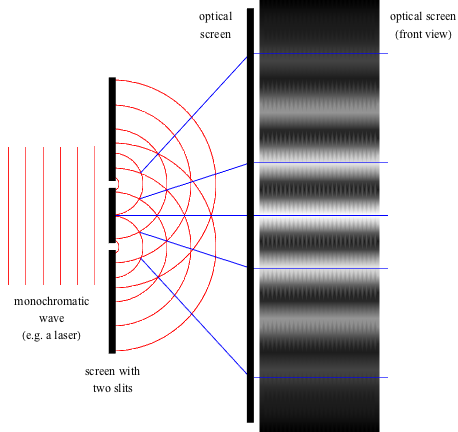
\includegraphics[width=0.6\textwidth,height=0.5\linewidth]{chapter1/img/younginterference.png}
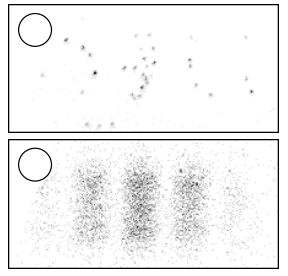
\includegraphics[width=0.4\textwidth,height=0.5\linewidth]{chapter1/img/doubleslitsinglephoton_crop.png}
\caption{\textit{Left:} Schematic view of interference pattern as in Young's experiment \cite{shmoop}.  \textit{Right:} (top) a single 20 ms time frame showing several individual photon arrival points; (bottom) image obtained after integrating for a few seconds: the diffraction pattern emerges \cite{weiswynands:2003}. }
\label{fig:doubleslit}
\end{figure}

In later years, similar experiments for electrons were done to prove the wavelike properties of particles \cite{Davisson:1927ta,thomson:1927}. The same double-slit experiment was finally perfomed in the 60s \cite{Jonsson1961} and for single electrons in 1974 \cite{merli:1974}. Single photon \cite{weiswynands:2003} (shown in Figure \ref{fig:doubleslit}) and single electron double-slit experiments show the same results, illustrating the wave probability interpretation of particles and fields.
\fi

\subsection{Predictions}
By 1932, scientists knew that atoms were made up by protons, neutrons and electrons. Together with the photon, a total number of four particles were known. Four grew to five when Anderson discovered the existence of positrons \cite{Anderson:1933mb} (predicted by Dirac \cite{Dirac:1928hu}). Then came the muon \cite{Neddermeyer:1937md} and pion \cite{Lattes:1947mw}. By the 1960s, there were ``fundamental particles'' with no good guiding principles to link them together. They were often referred to as the ``particle zoo''.

By a series of insights by several individuals, the Standard Model as a quantum field theory became more widely accepted. Since then, the model has predicted the results of experiment after experiment. Some of them are:

\vspace{2mm}

\begin{itemize}
\item Neutral weak currents. Postulated by Salam, Weinberg and Glashow, the theory of electroweak interactions predicted the existence of a new type of weak interaction, in which the reacting particles do not change their charges. The first observation was made in 1973 in the Gargamelle experiment at the European nuclear research laboratory, CERN \cite{Hasert:1973ff}.
\item Weak gauge bosons. Again postulated by the abovementioned people. These particles were discovered in the UA1 and UA2 experiments in CERN, 1983 \cite{Arnison:1983rp,Arnison:1983mk}.
\item Heavy quarks. To explain the $CP$-violations in kaon decays, M. Kobayashi and T. Maskawa predicted the existence of a third generation of quarks: the \textit{top} and \textit{bottom} quarks. The bottom quark was discovered in 1977 at Fermilab \cite{Herb:1977ek}. It took another 18 years for the top quark to be found in the same institute \cite{Abe:1995hr}. 
\item Gluons. The gauge bosons of quantum chromodynamics were discovered in 1978 and 1979 \cite{Barber:1979yr}.
\item Higgs boson. On July 4, 2012, physicists at CERN announced the discovery of the only fundamental particle predicted by the Standard Model that was not yet discovered. 
\end{itemize}  
\subsection{Precision tests}
%Below, a small subset of many precision tests is given: 

%\begin{itemize}
%\item \textit{Lamb shift}, a difference in energy between two energy levels of the hydrogen atom that was not predicted by the Dirac equation. This phenomenon is explained with the theory of QED. \textcolor{red}{REF}.
%\item \textcolor{red}{Andere goede voorbeelden? Precision measurements in IceCube? vb: Neutrino cross-section: IceCube/Nature https://www.nature.com/articles/nature24459}

%\end{itemize}

Inconsistencies between experiment and theory can be signs of wrong or incomplete theories. For this reason, experimentalists are continuously testing parameters of the SM. These precision tests are most often done by testing the theory of quantum electrodynamics (QED). With the use of \textit{renormalization theory}, many parameters of the theory can be calculated with high precision. High-precision measurements of various observables have been performed at LEP 1 and SLC \cite{ALEPH:2005ab,Riemann:2010zz,Abe:2000dq,Abe:2000uc,Abe:2000hk,Abe:1996ef} for physics at the $Z$-boson mass ($\sqrt{s} \approx M_Z$) and other observables at Tevatron \cite{Aaltonen:2013iut,TEW:2010aj}, LEP 2 \cite{TEW:2010aj}, ATLAS \cite{Aaboud:2017svj,ATLASurl1} and CMS \cite{CMSurl1,CMSurl2}. Some of them are listed in Table \ref{tab:precision}. The parameters in the table show that the SM best-fit predictions are very consistent with what we see in experiments.

\vspace{2mm}
\begin{itemize}
\item The SM predicts kaons to decay into charged pions and a neutrino-antineutrino pair to happen once every ten billion kaon decays. The SM fit to this decay has a small uncertainty, making the search interesting for possible anomalies. A candidate event of this very rare decay has been reported by the NA62 collaboration in 2018 but is in accordance with the SM predictions \cite{na62}.

\item Another example is the measurement of the \textit{Lamb shift}, a difference in energy between two energy levels of the hydrogen atom that was not predicted by the Dirac equation and currently provides a measurement of the fine-structure constant $\alpha$ to better than one part in a million, allowing a precision test of QED.

\item Electrons have a magnetic dipole moment as a result from their intrinsic spin. A charge distribution in these particles, which we do not expect to happen for fundamental particles, would make the electon charge not seem perfectly spherical. This electron electric dipole moment (EDM) is expected from the SM only with an extremely small value from radiative corrections with $CP$-violating interactions, at most $10^{-38}\ e \cdot \textrm{cm}$. Recent measurements from the ACME experiment set the current upper limit at a value of  $1.1 10^{-29}\ e \cdot \textrm{cm}$ \cite{Cesarotti:2018huy}.
\end{itemize}
\vspace{2mm}

\noindent There have been other, more challenging precision test, such as neutrino cross-section measurements \cite{Aartsen:2017kpd} and measurements of the top quark mass in the CMS experiment \cite{Castro:2017yxe}. Both are again in agreement with the SM.


\begin{table}[]
\centering
\caption{Observables compared with the SM best fit. Errors are the total (experimental plus theoretical) uncertainties. Results are taken from Tables 10.4 and 10.5 in \cite{PDG2018url}.}
\label{tab:precision}
\resizebox{\textwidth}{!}{%
\begin{tabular}{|l|c|c|c|}
\hline
\rowcolor[HTML]{F1A91E} \textbf{Parameter}                                                 & \textbf{Experimental value}                              & \textbf{Theoretical value}                               & \textbf{Standard deviation} \\ \hline
$m_t$ {[}GeV{]}                                           & $172.74 \pm 0.46$                               & $172.96 \pm 0.45$                               & -0.5              \\ \hline
                  & $80.387 \pm 0.016$                              & \multirow{3}{*}{$80.358 \pm 0.004$}             & 1.8               \\ \cline{2-2} \cline{4-4}
                                                  & $80.376 \pm 0.033$                              &                                                 & 0.6               \\ \cline{2-2} \cline{4-4}
\multirow{-3}{*}{$m_W$ {[}GeV{]}}                                  & $80.370 \pm 0.019$                              &                                                 & 0.6               \\ \hline
            & $2.046 \pm 0.049$                               & \multirow{2}{*}{$2.089 \pm 0.001$}              & -0.9              \\ \cline{2-2} \cline{4-4}
  \multirow{-2}{*}{$\Gamma_W$ {[}GeV{]}}       & $2.195 \pm 0.083$                               &                                                 & 1.3               \\ \hline
$m_H$ {[}GeV{]}                                   & $125.14 \pm 0.15$                                                 & $125.14 \pm 0.15$                               & 0.0               \\ \hline
$g^{\nu e}_V$                                             & $-0.040 \pm 0.015$                              & $-0.0398 \pm 0.0001$                            & 0.0               \\ \hline
$g^{\nu e}_A$                                             & $-0.507 \pm 0.014$                              & $-0.5063$                                       & 0.0               \\ \hline
$\tau_\tau$ {[}fs{]}                                      & $290.75 \pm 0.36$                               & $290.39 \pm 2.17$                               & 0.1               \\ \hline
$\frac{1}{2}\left(g_\mu - 2 - \frac{\alpha}{\pi} \right)$ & $\left( 4511.18 \pm 0.77\right) \times 10^{-9}$ & $\left(4508.63 \pm 0.03 \right) \times 10^{-9}$ & 3.3               \\ \hline
$M_Z$ {[}GeV{]}                                           & $91.1876 \pm 0.0021$                            & $91.1884 \pm 0.0020$                            & -0.4              \\ \hline
$\Gamma_Z$ {[}GeV{]}                                      & $2.4952 \pm 0.0023$                             & $2.4942 \pm 0.0008$                             & 0.4               \\ \hline
$\Gamma_Z (\textrm{had})$ {[}GeV{]}                                & $1.7444 \pm 0.0020$                             & $1.7411 \pm 0.0008$                             & -                 \\ \hline
$\Gamma_Z (\textrm{inv})$ {[}MeV{]}                                & $499.0 \pm 1.5$                                 & $501.44 \pm 0.04$                               & -                 \\ \hline
$\Gamma_Z \left(l^+ l^- \right)$ {[}MeV{]}                & $83.984 \pm 0.086$                              & $83.959 \pm 0.008$                              & -                 \\ \hline
\end{tabular}%
}
\end{table}



\section{The need for physics beyond the Standard Model}
\label{needforBSM}
Despite its incredible success, many physicists believe the Standard Model is certainly not the full story. There are a number of features that seem arbitrary, but also some that cannot be explained by the theory alone. Below, I give a list of open questions:

\vspace{2mm}

\begin{itemize}
\item Why are there \textbf{three families} for both leptons and quarks? Why  not two? Or four? Or even a thousand?
\item What is the \textbf{cause of the symmetries} we see in the Standard Model? Why is, for example, QCD not an SU(4) gauge theory?
\item There are a number of \textbf{parameters} in the SM that cannot be explained by first principles. We have no good explanation for why the top quark is 75 000 times heavier than the up quark. Why is the vev of the Higgs potential 246 GeV? Why is the Higgs mass 125 GeV? There are in total 26 parameters in the SM that are determined by experiments and can be found in Table \ref{tab:freeparameters}.
\item Why does the Higgs potential have this\textbf{ Mexican hat shape}? In other words, why is $\mu^2$ in $\lambda \left(\Phi^\dagger \Phi \right)^2 + \mu^2\left(\Phi^\dagger \Phi \right)$ negative? Also, the vev, the mass of the Higgs boson and the mass of the fermions due to the Yukawa couplings all appear in Table \ref{tab:freeparameters}. This makes us believe there is something we do not fully understand about the BEH mechanism. 
\item Right-handed neutrinos can be introduced into the SM. They are singlets with respect to the strong and weak interaction and would therefore not carry an electric charge, weak hypercharge or weak isospin. Due to this lack of charge, right-handed neutrinos would be extremely difficult to detect. They have Yukawa interactions with other leptons and the Higgs boson, but its coupling would be extremely small. Neutrinos can become massive with Dirac mass terms in the same way charged leptons become massive in the BEH mechanism. Their \textbf{extremely small masses} suggest another mechanism in which the very light left-handed neutrinos are accompanied with extremely heavy right-handed neutrinos. This mechanism is called the \textit{Seesaw mechanism} and requires the addition of Majorana mass terms.
\end{itemize}
\vspace{2mm}
\noindent Aside from these, there are a number of unexplained phenomena that probably cannot be explained in a simple extension of the Standard Model but need a non-trivial approach. For example:

\vspace{2mm}

\begin{itemize}
\item It is a natural assumption that the universe is neutral with all conserved charges. Both the SM and general relativity give no explanation for the \textbf{matter-antimatter imbalance} we see in the universe. The Big Bang was expected to produce equal amounts of matter and anti-matter, yet we see that the observable universe consists almost exclusively out of baryonic matter\footnote{Why are there protons, neutrons and electrons everywhere while it is perfectly possible for antiprotons and antineutrons to form atomic nuclei with positrons?}. The most likely explanation is that in the early universe physical laws we know today were absent or have acted differently. The observed $CP$-violation is insufficient to account for the observed baryon asymmetry of the universe given the limits on baryon number violation.
\item The stars, planets, interstellar clouds, etc. we see in space consist of baryonic matter. Assuming general relativity is the correct theory to describe gravity on cosmological scales, the Lambda-CDM model predicts that the matter we see is only around 15\% of the total matter present in our visible universe \cite{Ade:2015xua}. To explain the galaxy rotation curves \cite{Corbelli:1999af}, galaxy velocity dispersions \cite{Faber:1976sn}, galaxy cluster masses \cite{Allen:2011zs}, gravitational lensing \cite{Natarajan:2017sbo}, and many more, it is predicted that around 85\% of the mass is not yet observed. This matter is referred to as \textbf{dark matter} as it cannot interact electromagnetically because it would have already been observed otherwise. No known particles in the SM can explain this phenomenon.
\item Similar to dark matter, the Lambda-CDM model predicts that the total energy in the visible universe should consist mostly out of a constant energy density for the vacuum called \textbf{dark energy}. 5\% of the total energy consists of baryonic matter, 26\% should be dark matter and the remaining 69\% of dark energy is necessary to explain the expansion of the universe\footnote{If there is only matter and the Big Bang acceleration only happened in the beginning of the creation of the universe, then one would expect the expansion to diminish due to the gravitational pull of matter. Measurements say the opposite is true: the universe is expanding and in an accelerating rate.}.
\item General relativity is generally accepted to describe gravity on cosmological scales. Thusfar, it has not been possible to describe \textbf{gravity} on a quantum scale, as is the case for the Standard Model, and still be valid on very large scales. The inclusion of the graviton would for example not recreate what is observed experimentally without other modifications to the SM, which have not been observed. There is a need for a more complete theory beyond the range of their combined applicability \cite{Donoghue:2012zc}.
\item Why is the $CP$-violation in the strong interaction extremely small or even zero?
\item Often referred to as the muon g-2 anomaly, there are possible hints of new physics as the theoretical prediction of magnetic moment of the muon and experimental values have a small but significant offset (see Table \ref{tab:precision}).
\item Why is there much more mixing in the lepton sector (PMNS) compared to the quark sector (CKM)? 
\item To explain the apparent quantum fluctuations on cosmological scales together with the horizon, flatness and magnetic monopole \cite{McCoy:2015bra} problems, we have a theory of exponential expansion of space in the early universe: \textbf{cosmic inflation}. The theory states that between $10^{-36}$ and $10^{-32}$ seconds after the Big Bang, a rapid exponential expansion happened. This could explain the apparent thermal equilibrium between parts of the visible universe that are not in causal contact with each other and the even distribution of the cosmic microwave background. The hypothetical field that is thought to be responsible for inflation, the inflaton field, is not observed and would be an extension of the Standard Model.
\item With the use of renormalization theory, it is possible to show that bare parameters should not be the same as parameters measured in experiments. These parameters, such as the mass of particles, depend on the energy scale at which they are probed and physics far beyond the scope of the probed energy scale can influence these parameters. An example are the screening and anti-screening effects. If one believes that all forces can be described by one theory at higher energies, these constants can converge at higher energy scales which is not the case when extrapolating these parameters as can be seen in Figure \ref{fig:running}.

Similarly, one-loop corrections to the Higgs boson mass\footnote{Fermions and bosons are not affected by higher energy physics in the same way as a scalar particle is.} will have radiative corrections with a quadratic dependence on the cutoff scale. Virtual particles in one-loop corrections can have infinite momenta that should contribute to the total mass of the Higgs boson. Since we expect new physics to be present at energies close to the Planck mass ($\approx 10^{18}$ GeV), these loop corrections should push the Higgs mass to similar energy ranges. But, we see that the Higgs mass is around 125 GeV. This would mean that there are other parameters which should almost \textit{exactly} cancel these absurdly large numbers. This is called \textit{fine-tuning}, and it's the intuition of most physicists that this incredible fine-tuning has a deeper, yet unknown, meaning. This problem is often referred to as the \textbf{hierarchy problem}.
\end{itemize}




% Please add the following required packages to your document preamble:
% \usepackage[table,xcdraw]{xcolor}
% If you use beamer only pass "xcolor=table" option, i.e. \documentclass[xcolor=table]{beamer}
\begin{table}[]
\caption{The 26 free parameters in the Standard Model that have to be measured experimentally.
%Including neutrino masses and the PMNS mixing angle, 7 new parameters have to be added: $m_{\nu_1},m_{\nu_2},m_{\nu_3}$, the mixing angles $\theta_{12},\theta_{13}$ and $\theta_{23}$ and the $CP$-violating phase $\delta_{CP}$.
}
%from wikipedia: standard model
\label{tab:freeparameters}
\centering
\resizebox{\textwidth}{!}{%
\begin{tabular}{|l|c|c|c|c|}
\hline
\rowcolor[HTML]{F1A91E} 
\cellcolor[HTML]{F1A91E}\textbf{Parameter}      & \textbf{Description}                    & \textbf{Value}        & \textbf{Uncertainty} & \textbf{Reference} \\ \hline
$m_e$          & Electron mass                  & 511 keV      & $\pm 3.1 \cdot 10^{-6}$ keV  & \cite{PDG2018url}\\ \hline
$m_\mu$        & Muon mass                      & 105.7 MeV    & $\pm 2.4\cdot 10^{-6}$ MeV & \cite{PDG2018url} \\ \hline
$m_\tau$       & Tau mass                       & 1.78 GeV     & $\pm 1.2 \cdot 10^{-4}$ GeV & \cite{PDG2018url}\\ \hline
$m_u$          & Up quark mass                  & 2.2 MeV      & $\left[-0.4, +0.5\right]$ MeV & \cite{PDG2018url}\\ \hline
$m_d$          & Down quark mass                & 4.7 MeV      & $\left[-0.3, +0.5\right]$ MeV & \cite{PDG2018url} \\ \hline
$m_c$          & Charm quark mass               & 1.275 GeV     & $\left[-0.035, +0.025\right]$ GeV& \cite{PDG2018url} \\ \hline
$m_s$          & Strange quark mass             & 95 MeV       & $\left[-3, +9\right]$ MeV & \cite{PDG2018url}\\  \hline
$m_t$          & Top quark mass                 & 173.0 GeV    & $\pm 0.4$ GeV & \cite{PDG2018url}\\ \hline
$m_b$          & Bottom quark mass              & 4.18 GeV     & $\left[-0.03, +0.04\right]$ GeV & \cite{PDG2018url}\\ \hline
$\theta_{12,\textrm{CKM}}$  & CKM 12-mixing angle            & 13.04$^\circ$ & $\pm 0.05^\circ$ & \cite{PDG2018url}\\ \hline
$\theta_{23,\textrm{CKM}}$  & CKM 23-mixing angle            & 2.38$^\circ$  & $\pm 0.06^\circ$ & \cite{PDG2018url}\\ \hline
$\theta_{13,\textrm{CKM}}$  & CKM 13-mixing angle            & 0.201$^\circ$  & $\pm 0.011^\circ$ & \cite{PDG2018url}\\ \hline
$\delta_{CP,\textrm{CKM}}$  & CKM CP violation phase         & 1.20 rad   & $\pm 0.08$ rad & \cite{PDG2018url}\\ \hline
$\alpha^{-1} (M_Z)$ & Electromagnetic coupling constant $^*$ & 127.955 & $\pm 0.010$ & \cite{PDG2018url}\\ \hline
$\sin^2 \theta_W (M_Z) $ & Weinberg angle $^*$ & 0.23122 & $\pm 3\cdot 10^{-5}$ & \cite{PDG2018url}\\ \hline
$\alpha_s \left(M_Z\right)$ & Strong coupling constant $^*$  & 0.1187  & 0.0016 & \cite{PDG2018url}\\ \hline
$\theta_{QCD}$ & QCD vacuum angle    & $< 10^{-9}$  & / & \cite{Peccei:2006as}\\ \hline
$v$            & Higgs vacuum expectation value & 246 GeV      & / & \cite{AMSLER20081}\\ \hline
$m_H$          & Higgs mass                     & 125.09 GeV      & $\pm 0.21 \textrm{(stat)},\pm 0.11 \textrm{(syst)}$ GeV & \cite{Aad:2015zhl}\\ \hline
 &   & \multirow{6}{*}{\begin{tabular}[c]{@{}c@{}} $\sum_i m_{\nu i} < 120 $ meV\\ \\$\frac{\Delta m^2_{21}}{10^{-5}\textrm{eV}^2} = 7.39$\\ \\ $\frac{\Delta m^2_{31}}{10^{-3}\textrm{eV}^2} = 2.525 $\end{tabular}} & \multirow{6}{*}{\begin{tabular}[c]{@{}c@{}}95\% C.L.\\ \\$\left[-0.20,+0.21 \right]$\\ \\ $\left[-0.032,+0.033 \right]$\end{tabular}}  & \multirow{6}{*}{\begin{tabular}[c]{@{}c@{}} \cite{Mertens:2016ihw}\\ \\ \cite{Esteban:2016qun,nufit2018} \\ \\ \cite{Esteban:2016qun,nufit2018} \end{tabular}}\\
\multirow{-2}{*}{$m_{\nu1}$} &\multirow{-2}{*}{Neutrino mass parameter}&&&\\
 &     &       & & \\
\multirow{-2}{*}{$m_{\nu2}$} &\multirow{-2}{*}{Neutrino mass parameter}&&&\\ 
 &   &       & & \\ 
\multirow{-2}{*}{$m_{\nu3}$} &\multirow{-2}{*}{Neutrino mass parameter}&&&\\
\hline
$\theta_{12,\textrm{PMNS}}$  &  PMNS 12-mixing angle$^\dagger$ & $33.82^{\circ}$ & $\left[-0.76^\circ, +0.78^\circ \right]$ & \cite{Esteban:2016qun,nufit2018}\\ \hline
$\theta_{23,\textrm{PMNS}}$  &  PMNS 23-mixing angle$^\dagger$ &
$49.6^{\circ}$ & $\left[-1.2^\circ, +1.0^\circ\right]$ & \cite{Esteban:2016qun,nufit2018}\\ \hline 
$\theta_{13,\textrm{PMNS}}$  &  PMNS 13-mixing angle$^\dagger$ &$8.61^{\circ}$ & $\left[-0.13,+0.13^\circ\right]$ & \cite{Esteban:2016qun,nufit2018}\\ \hline
$\theta_{CP,\textrm{PMNS}}$  &  PMNS CP violation phase$^\dagger$ &  $215^{\circ}$ & $\left[-29^\circ,+40^\circ \right]$ & \cite{Esteban:2016qun,nufit2018} \\ \hline
\end{tabular}%
}
$^*$ The coupling constants depend on the energy scale: ``running of the coupling constants''.\\
$^\dagger $ Assuming normal mass ordering, for inverted ordering see reference.
\end{table}
\vspace{2mm}


\noindent Many of these problems can be seen as unwarranted. Why there are three families and why so many parameters in the Standard Model have no fundamental explanation could just be because it's just the way it is. Maybe there is a multiverse, a plethora of universes with similar Standard Models, which have slightly or vastly different parameters. Some questions might even be impossible to answer because of a lack of statistics: we only have one universe and mankind has not been around very long in the timescale of the universe. This consideration might be valid but again doesn't answer all our questions, it does not solve the question of dark matter for example.

This argumentation should not prevent us to try and find a more general theory for the Standard Model and general relativity. A better explanation could be fairly simple, but infinitely hard as well. There is only one way in trying to find a better understanding: experiments.

Unification is the most popular approach in describing physics beyond the Standard Model. Unification would mean that well-established theories are low-energy approximations of a more grand unified theory. Historically, this has worked very well: the unification of celestial gravitation of Kepler with terrestrial gravitation of Galileo into universal gravitation and the unification of electricity, magnetism, and later optics into electromagnetism. Gravity was overhauled by the much broader theory of general relativity. Lastly, the birth of gauge theories have combined QED and the weak interaction into the combined electroweak theory. The similarities in QCD and the electroweak theory, both being gauge theories, has led people to believe a unification is possible. This would unify the forces and particles known from the Standard Model into a \textit{Grand Unified Theory} or GUT. A theory that would add gravity is called a \textit{Theory Of Everything} or TOE.

%START LEAVING OUT
\iffalse
\subsection{Running of the coupling constants}
\label{subsec:running}
The coupling constants in the Standard Model are actually not constants. They depend on the energy of the system. Quantum fluctuations in vacuum have a non-negligible contribution in the apparent charge of particles. The effects of screening and anti-screening are visualized in Figure \ref{fig:screening} and can be mathematically formulated as a beta function. The function encodes the dependence of a coupling parameter, $g$, on the energy scale $\mu$:


\begin{figure}
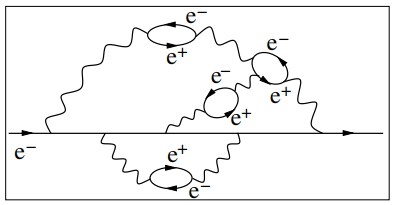
\includegraphics[width=0.5\textwidth,height=0.3\textwidth]{chapter1/img/screening}
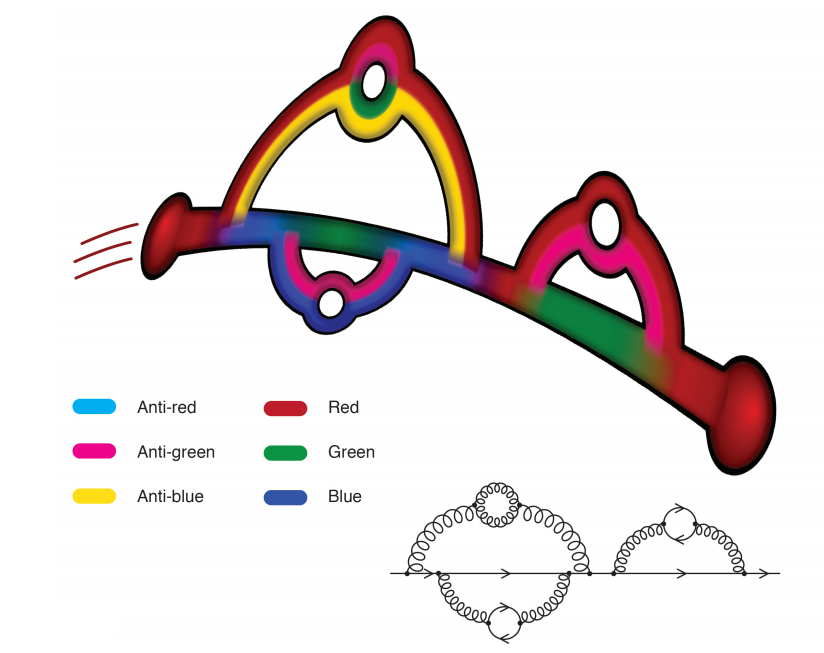
\includegraphics[width=0.5\textwidth,height=0.3\textwidth]{chapter1/img/antiscreening}
\caption{\textit{Left}: virtual pairs of positrons and electrons can be produced in vacuum. Positrons are attracted to the bare electron resulting into an apparent lower charge of the bare particles from larger distances. This effect is referred to as \textit{screening}. \textit{Right}: quark and antiquark pairs have a similar screening effect in color charge as the case for electrical charges. There is an anti-screening effect due to gluons that ``extract'' color from the bare quark and is stronger than the screening effect of quark-antiquark pairs. At small distances, the dilution of the initial color charge is larger than at large distance.  This drawing should not be taken literally and the concept of self-interaction is very hard to illustrate. One could interpret the initial red color with a gluon emission as a conservation of the red color, thus the red quark can only become blue if a gluon with a red and anti-blue color is emitted (gluons need to be color+anti-color pairs). In the first, top loop, two  gluons are created but cannot have a combined color: anti-green with red (first) and green with anti-blue (second) is possible since green and anti-green have a net zero color charge. Figures from \cite{Deur:2016tte}.}
\label{fig:screening}
\end{figure}

\begin{equation}
\beta\left(g\right) = \frac{\partial g}{\partial \log\left(\mu\right)}.
\end{equation}
More coupling in shorter distances (i.e. higher energies) would give rise to a positive beta function and is the case in QED. In QCD, gluons carry a color charge and enter the beta function with a negative sign

\begin{equation}
\beta\left(g\right) = -\left(11 - \frac{2n_f}{3}\right)\frac{g^3}{16\pi^2},
\end{equation}
with $n_f$ the number of fermions that participate in the strong interaction. This decrease in coupling strength in function of energy scale is called \textit{asymptotic freedom}. Alternatively, we can write down the coupling constants in function of the energy 

\begin{equation}
\alpha^{-1}_i \left(Q\right) = \alpha^{-1}_{i}\left(m_Z\right) + \frac{b_i}{2\pi}\log\frac{Q}{m_Z},
\end{equation}
with $b_1 = -\frac{4}{3}n_g - \frac{1}{10}n_h$, $b_2 = \frac{22}{3}-\frac{4}{3}n_g-\frac{1}{6}$ and $b_3 = \frac{11}{-\frac{4}{3}}$ the U(1), SU(2) and
SU(3) constants in which $n_g$ denotes the  number of quark and lepton generations and $n_h$ is the number of Higgs doublet fields. These three couplings seem to converge, leading people to believe a more universal theory at higher energies would unify these parameters into one and is shown in Figure \ref{fig:running}.
\fi
%END LEAVING OUT

\begin{figure}
\centering
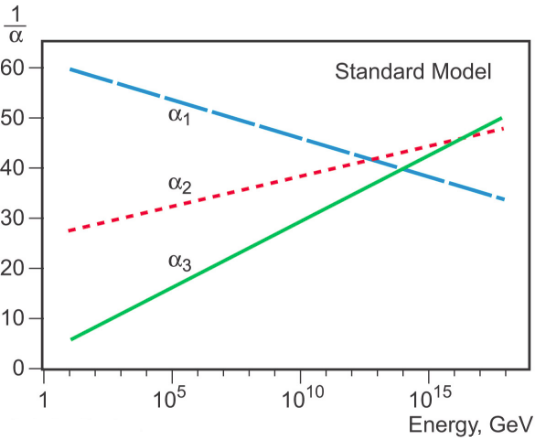
\includegraphics[width = 0.5\textwidth]{chapter1/img/running}
\caption{Running of the coupling constants in the Standard Model. Figure from \cite{nobel2004url}.}
\label{fig:running}
\end{figure}

\subsection{Unifying theories}
\label{sub:unifying}
Linking the seemingly arbitrary parameters in the Standard Model has been ongoing for the last couple of decades. Combining these theories is not straightforward since they exhibit very different behaviors. Electromagnetism is long-ranged, the weak force is short-ranged and the strong force is weak in high-energy environments such as the early universe and strong where the probing energy is low. Many GUTs predict that quarks and leptons are part of a single representation of a gauge group with one single hypercharge and would explain why the electric charge of electrons and protons seem to be exactly the same \cite{He:1989eq}.

The simplest GUT is SU(5), which would break down into the Standard Model at lower energies due to spontaneous symmetry breaking. Other possible extensions are, for example, SO(10) \cite{Bertolini:2009qj}, SU(8) \cite{Yu:1984pb} and O(16) Lie groups. Another example is string theory, a theoretical framework that starts with the idea that point-like particles of particle physics can be replaced by one-dimensional objects called strings. These strings can propagate through space and interact with each other. Properties that we are more familiar with, such as charge, mass, etc. are determined by the vibrational state of the strings.

Unfortunately, the full theory does not have a definition in all circumstances and describes an enormous landscape of possible universes and is mainly used to describe quantum gravity. However, charge quantization is often not assumed in string theory, making particles with an anomalous charge plausible \cite{Wen:1985qj,Athanasiu:1988uj}.\\


\noindent Without experimental results there is still much ongoing debate into which theory is the correct one. There are many more theories aside from the possible extentions that are listed here such as Supersymmetry, Little Higgs, Technicolor... but go beyond the scope of this work.

\iffalse
\subsubsection*{Supersymmetry}
Supersymmetric models impose a new symmetry, supersymmetry (SUSY), that relates fermions and bosons. Every fermion would have a, yet unseen, bosonic supersymmetric partner and vice versa. This theory is highly motivated due to its ability in canceling the quadratically divergent terms in the mass correction of the Higgs boson. More specifically, because the Higgs couples to massive particles there will be a correction to the bare Higgs mass due to these couplings. By applying the Feynman rules, the quantum corrections to the Higgs mass squared from fermions is 

\begin{equation}
\label{eq:higgscorrections}
\Delta m^2_H = -\frac{\left| \lambda_f \right|^2}{8\pi^2} \left[ \Lambda^2_{UV}+...\right],
\end{equation}
\noindent where $\Lambda_{UV}$ is the ultraviolet cutoff. If we assume this to be of the order of the Planck mass, this would lead to extremely small numbers for the Yukawa coupling constants $\lambda_f$.

Alternatively, the corrections from two additional complex scalors with similar couplings to the Higgs ($\lambda_s = \left|\lambda_f\right|^2$) is equal to

\begin{equation}
\Delta m^2_H = 2 \times \frac{\lambda_s}{16\pi^2}\left[ \Lambda^2_{UV}+... \right]
\end{equation}
and are able to cancel the fermion contributions. Unbroken SUSY would lead to partners with the same mass as the particles we know from the SM and would have been discovered long ago. Because of this, one assumes the symmetry to be broken.

The last couple of years, SUSY was regarded as the most promising extension of the SM with tremendous efforts from big collaborations such as the experiments at the Large Hadron Collidor (LHC) in search for proof. Unfortunately, to this date no evidence for SUSY has been found.

\subsubsection*{Little Higgs}
The basic motivation for a Little Higgs scenario comes from the quadratic one-loop corrections such as in Eq. \ref{eq:higgscorrections}. In Little Higgs scenarios, the Higgs field is a pseudo-Nambu-Goldstone boson of a spontaneously broken symmetry. The symmetry is broken by two sets of interactions and each interaction preserves enough symmetry so that no single interaction gives radiative corrections to the Higgs mass. However, two interactions together do generate a Higgs mass, but the Higgs mass squared terms are suppressed by two loops relative to the cutoff. Because these are proportional to the two coupling strengths, while the Standard Model Higgs only requires a single interaction to generate a mass, it has a lower radiative mass corrections compared to the Standard Model Higgs. The biggest difference in Little Higgs scenarios with Supersymmetry is that it has particles of the same spin that cancel the quadratic divergences to the Higgs mass, i.e. a fermion cancels a quadratic divergence from a fermion. For more information, see Refs. \cite{Cheng:2007bu,Reuter:2012sd}.	

\subsubsection*{String theory}

\fi




\subsection{How to look for new physics}
In general, one could say there are two possible ways to look for new physics. Essentially all of the physics in our solar system can be explained with what we know from the Standard Model. Interactions in controlled laboratory environments are currently on the order of $\sim$10 TeV center of mass energy in the experiments at the LHC. This could still be well below the energy levels to produce new, exotic, particles. In the \underline{energy frontier} it is the goal to reach the highest energies possible in order to get as close to the energy requirements where new physics becomes more prominent. As a consequence, more and more cosmic ray experiments have found an interest in searches for physics beyond the Standard Model. This is sometimes called the \textit{cosmic frontier}. This analysis tries to explore this possibility in more detail for the IceCube experiment. Cosmic ray experiments have the disadvantage that they are not fully contained experiments and information is lost as the primary interaction is unknown and important parameters such as energy, direction, type,... of the particle have to be reconstructed with large uncertainties.

The other approach tries to extract information from precision experiments and is therefore reliant on lowering the statistical and systematical uncertainties. In these experiments, the intensity of the beam of particle accelerators is pushed to its highest value and this is therefore referred to as the \underline{intensity frontier}. This strategy tries to generate huge numbers of particles needed to study rare or exotic subatomic processes. Rare processes could give us a lot of information on unknown physics. Some parameters which can be calculated in the SM have a small offset with respect to what is measured in experiments.

The difference between the two methods can be summarized by saying that new physics at higher energies can produce new particles at high-energy collisions that are sought for in the energy frontier. The higher the scale where new physics enters, the more energy is needed in particle collisions. However, parameters from our current theories that not include new physics could also have a small but measurable offset at lower energies (the ones we are able to probe currently), which is what is measured in the intensity frontier. \\


\noindent I'd like to finish this chapter with quotes from Steven Weinberg in an interview with Nova about his vision on string theory. It shows the apparent stalemate physicists seem to find themselves in: there are no theoretical breakthroughs regarding long standing problems.

\begin{center}
\begin{minipage}[5cm]{0.9\textwidth}
\textit{``I believe that there is a simple theory that governs everything—the four forces we know about, perhaps other forces as well. I'm not sure that's true. It may be that nature is irreducibly messy. I'm sure that we should assume it's not, because otherwise we're never going to find a fundamental theory. But even so, we're not guaranteed that we'll find it. We may not be smart enough. Dogs are not smart enough to understand quantum mechanics. I'm not sure that people are smart enough to understand the whatever-it-is that unifies everything. I think we probably are, because of our ability to link our minds through language, but I'm not certain.''}
\end{minipage} 
\end{center}

\begin{center}
\begin{minipage}[5cm]{0.9\textwidth}
\textit{\noindent ``There was a marvelous period from, I'd say, the mid-'60s until the late '70s when theoretical physicists actually had something to say that experimentalists were interested in. Experimentalists made discoveries that theoretical physicists were interested in. Everything was converging toward a simple picture of the known particles and forces, a picture that eventually became known as the Standard Model. I think I gave it that name. And it was a time when graduate students would run through the halls of a physics building saying they had discovered another particle and it fit the theories, and it was all so exciting.''}
\end{minipage} 
\end{center}

\begin{center}
\begin{minipage}[5cm]{0.9\textwidth}
\textit{\noindent ``Since the late '70s, I'd say, particle physics has been in somewhat of a doldrums. Partly it's just the price we're paying for the great success we had in that wonderful time then. I think cosmology now, for example, is much more exciting than particle physics. The string theorists are trying to push ahead without much support from relevant experiments, because there aren't any relevant experiments that can be done at the kind of scales that the string theorists are interested in.''}
\end{minipage} 
\end{center}

\noindent Even though it might take us a long time to find the answers we are looking for, this current stalemate should not prevent us doing more fundamental research. We still do not know everything and it's probably even foolish to think we almost do. Finding some answers might be difficult but probably all the more fulfilling once we have them.

%----------------------------------------------------------------------------------------
%	CHAPTER 2
%----------------------------------------------------------------------------------------
\chapterimage{Exploring_the_unknown_2} % Chapter heading image
\chapter{Motivation of the Analysis}
\label{ch:theoreticalmotivation}
\begin{flushright}
\textit{\\The world is divided into people who think they are right $\sim$ Anonymous\\}
\end{flushright}

\noindent As seen in Chapter \ref{ch:SM}, there is an ongoing debate which beyond-the-Standard-Model physics models could help explain questions we do not have answers for. Over the last decades, this quest has proven to be non-trivial since many accelerator experiments have not given any clear hints towards physics that cannot be explained by the Standard Model. A big part of the physics community is trying its best to help answer these riddles and dedicated experiments have been constructed in the search for new physics. Other collaborations try to make use of their detector in the most efficient way possible. These experiments most often try to look for BSM physics by searching for signals in their detector that could not be explained by the particles we know today. One example, and also the subject of this work, is to try to look for particles that have a lower electromagnetic, but non-zero, charge than the charged particles of the Standard Model.

\section{Introduction}
As seen in Chapter \ref{ch:SM}, all free particles have an electromagnetic charge that is a multiple of the absolute electron charge, $e$, equal to $1.602 \times 10^{-19}$ C. Elementary particles such as (anti)quarks have fractional charges equal to $\pm\frac{1}{3}e$ and $\pm\frac{2}{3}e$, but have never been seen as isolated particles due to \textit{confinement} as explained in Section \ref{sub:quarks}. No other particles are expected to have a charge lower than $e$ and are therefore perfect candidates for searches beyond the Standard Model. Different experiments have sought these anomalously charged particles, which are referred to as \textit{Lightly Ionizing Particles (LIPs)} or \textit{Stable Massive Particles (SMPs)}. Throughout this work the latter denomination is used, indicating they do not rapidly decay and have masses significantly higher than the lightest leptons.

\section{Theory}
In Section \ref{sub:unifying}, possible extensions of the Standard Model were already introduced. One of the simplest possible extensions of the SU(3) $\times$ SU(2) $\times$ U(1) groups is the SU(5) gauge group. It is the smallest Lie group that can contain the group of the Standard Model without introducing any new fermions. It could explain charge quantization \cite{He:1989eq}, has complex representations and can accommodate fractional charges. In this scheme, new vector bosons, usually called $X$ and $Y$ bosons, occur with charges $\frac{4}{3}$ and $\frac{1}{3}$. Extensions of the SU(5) models allow for color singlet particles with charges $\frac{1}{3}$ and $\frac{2}{3}$ \cite{Barr:1982vj}. Other possible extensions are based on the SU(7) \cite{Frampton:1982gc}, SU(8) \cite{Yu:1984pb}, SO(14) \cite{Yamamoto:1982sk}, SO(18) \cite{Dong:1983nh}, SO(10) $\times$ SO(8) groups \cite{Jiang:1985jy}. 

It should be noted that the simplest form of an SU(5) gauge group is already highly constrained as proton decay is allowed in this model and estimated to be around $10^{30}-10^{31}$ years. However, experimental results have shown the lifetime to be $>1.6 \times 10^{34}$ years $\left(\tau\left(p \rightarrow \pi^0 e^+\right)\right)$ and $>7.7 \times 10^{33}$ years $\left(\tau\left(p \rightarrow \pi^0 \mu^+\right)\right)$ \cite{Miura:2016krn}.\\
\newline
There are also some string theories where massive particles with a fractional charge are predicted \cite{Wen:1985qj,Antoniadis:1992eb}. This was later confirmed to occur very often in certain compactifications \cite{Athanasiu:1988uj}.\\

\noindent More recently, there has been an increasing interest in searches for millicharged particles. New particles could couple to the Standard Model via a ``kinetic mixing'' or ``hypercharge portal'' \cite{Holdom:1985ag,Izaguirre:2015eya}. And in recent years, they were studied as possible candidates for dark matter \cite{Brahm:1989jh,Boehm:2003hm,Pospelov:2007mp,Bjorken:2009mm}. However, the charges of these particles are often $<10^{-3}e$ and therefore no ideal candidates in neutrino Cherenkov experiments. It is possible to look for them in neutrino experiments \cite{Magill:2018tbb}, but more targeted toward future experiments such as DUNE \cite{Acciarri:2015uup} and SHiP \cite{Anelli:2015pba}. A more detailed explanation of these particles can be found in Ref. \cite{Battaglieri:2017aum}. The most stringent upper limit in millicharged particles known to the author is given in Ref. \cite{Alvis:2018yte}.\\

\noindent There are many other possible extensions, but these go beyond the scope of this work. One should just keep in mind that no free particles with an anomalous charge less than $e$ are expected in the SM and that, if seen, they give clear hints of beyond-the-Standard-Model physics and would help in finding a more clear picture of what is possibly hidden beyond the realms of our understanding.


%\url{https://ac.els-cdn.com/S0370269314001257/1-s2.0-S0370269314001257-main.pdf?_tid=7f8b3af4-8845-417fa219-703f382cb092&acdnat=1535556263_162a6333d0a615412be21aa5fc3e5720
%}



\section{Previous searches}
\label{sec:prevsearches}
There are several ways one can assume to produce fractional charge particles. Different assumptions lead to different possible searches with previous and current detectors. In the following, the results of several experiments are shown. Accelerator and fixed target experiments look for particles that might be created in particle collisions, resulting in upper limits for production cross sections if no candidate events are found. Telescope experiments, on the other hand, often assume a flux of incoming particles that is bound to an upper limit if no candidate events are found.
%More information and a very good overview can be found in ..... diee summarypaper????

\subsection{Searches with accelerators and fixed targets}
The total energy of the interaction should be large enough to produce particles of a certain mass. The square of the centre of mass energy is given by:

\begin{equation}
\label{eq:totalenergy}
\begin{split}
s &= \left(p_1 + p_2\right)^2\\
&= m_1^2 + m_2^2 + 2E_1E_2 - 2\vec{p_1}\vec{p_2},\\
\end{split}
\end{equation}
where $p_{1,2}$ are the four-momenta of the two particles and $c$, the speed of light, is set to 1 in natural units.
Assuming $E$ is the energy of the incoming particle with mass $m_i$ and $m_t$ the mass of a target particle in rest and $E >> m_t, m_i$, the maximal mass reach of a search is given by:

\begin{equation}
\label{eq:mmax}
m_{max} \approx \sqrt{2 m_t E}.
\end{equation}
If $I$ is the incoming particle from the input beam and $N$ a nucleus, the production of exotic particles can then be denoted as

\begin{equation}
I + N \rightarrow F + X,
\end{equation}
where $F$ stands for the fractional charged particle and $X$ for the other particles that are produced in the interaction. No experiments that used accelerators and fixed targets found evidence for the existence of fractional charge particles \cite{Lyons:1984pw}. The highest-energy search used muons with a beam energy of 200 GeV, resulting in an $m_{max}$ of 19 GeV \cite{Aubert:1983jy}.
\subsection{Colliders}
Particle colliders can reach much higher energies than most fixed-target experiments. We see from Eq. \ref{eq:totalenergy} that the maximal mass of new particles in a storage ring that is colliding particles of energy $E$ with $E>>m_1,m_2$ scales with the energy: 

\begin{equation}
\begin{split}
&s = 4E^2,\\
\rightarrow \ &m_{max} = 2E
\end{split}
\end{equation}
There is a big difference in lepton and hadron accelerator experiments since much less particles are being produced in the former due to the absence of strong interactions. The production is ``cleaner'' and the particles sought are easier to distinguish from other productions. But, it is more difficult to reach higher energies for lepton accelerators\footnote{The radiative power of synchrotron radiation scales with a factor of $m^{-4}$: particles with low mass lose much more energy in circular accelerators with a fixed radius.}. An overview of electron-positron colliders is given in Table \ref{tab:elecposcollider}. No evidence for fractionally charged particles was found.


\begin{table}[]
\caption{Highest-energy fractional charge particle searches in electron-positron colliders. No evidence for fractionally charged particles was found.}
\label{tab:elecposcollider}
\centering
\begin{tabular}{|l|c|c|c|}
\hline
\rowcolor[HTML]{F1A91E} 
\textbf{$\sqrt{s}$ (GeV)} & \textbf{Charges sought}                        & \textbf{Collider} &\textbf{Reference}\\ \hline
1-1.4		 & $\frac{2}{3}$						 & VEPP-2M  & \cite{Bondar:1985sb} \\ \hline
29			 & $\frac{1}{3},\frac{2}{3}$			 & PEP & \cite{Aihara:1984px} \\ \hline		
130-209      & $\frac{2}{3},\frac{4}{3},\frac{5}{3}$ & LEP & \cite{Abbiendi:2003yd}    \\ \hline
130-136, 161 and 172 & $\frac{2}{3}$                 & LEP & \cite{Abreu:1996py}    \\ \hline
91.2 ($m_Z$) & $\frac{2}{3},\frac{4}{3}$             & LEP & \cite{Akers:1995az}    \\ \hline
91.2 ($m_Z$) & $\frac{4}{3}$   	    			     & LEP & \cite{Buskulic:1992mr}  \\ \hline
\end{tabular}
\end{table}

Experiments that use proton-antiproton colliders have reached larger masses but have also found no evidence of fractionally charged particles. An overview is given in Table \ref{tab:protonantiprotoncollider}.


\begin{table}[]
\caption{Highest-energy fractional charge particle searches in proton-(anti)proton colliders. No evidence for fractionally charged particles was found.}
\label{tab:protonantiprotoncollider}
\centering
\begin{tabular}{|l|c|c|c|c|}
\hline
\rowcolor[HTML]{F1A91E} 
\textbf{$\sqrt{s}$ (GeV)} & \textbf{Type} & \textbf{Charges sought}            & \textbf{Collider} & \textbf{Reference} \\ \hline
540		 & $p\overline{p}$ & $\frac{1}{3},\frac{2}{3}$ & SPS      & \cite{Banner:1985ev} \\ \hline
1800          & $p\overline{p}$ & $\frac{2}{3},\frac{4}{3}$ & Tevatron & \cite{Abe:1992vr}         \\ \hline
1800          & $p\overline{p}$ & $\frac{1}{3},\frac{2}{3}$ & Tevatron & \cite{Acosta:2002ju} \\ \hline
7000          & $pp$ & $\frac{1}{3},\frac{2}{3}$ & LHC & \cite{CMS:2012xi} \\ \hline

\end{tabular}
\end{table}

A more recent search was performed at the LHC, a proton-proton collider, when operating at a center of mass energy of 7 TeV. No evidence of particles with fractional charge was found. An upper limit of 95\% confidence level was set for particles with electric charge $\frac{2}{3}$ up to a mass of 310 GeV and 140 GeV for those with charge $\frac{1}{3}$ \cite{CMS:2012xi}.

\subsection{Searches for particles with telescopes}
There are several ways that particles with a fractional charge could be produced in cosmological events;

\vspace{2mm}
\begin{itemize}
\item the particles were produced early on in the Universe and are a stable component of the present matter;
\item the particles are rare but can be continuously produced in high-energy astrophysical events; or
\item the particles are produced in cosmic ray processes near Earth.
\end{itemize}
\vspace{2mm}

\noindent Because there is no clear preference for one of these possibilities, most telescope experiments express their search sensitivity as an incoming flux close to the detector in units of [cm$^{-2}$ s$^{-1}$ sr$^{-1}$]. This analysis has adopted the same search strategy and aims to improve on previous results. The most stringent upper limit was realized by the MACRO experiment found on the arXiv (not published, Ref. \cite{Ambrosio:2004ub}) that compares results from older searches and can be seen in Figure \ref{fig:upperlimits}. The best published result is set by Kamiokande II with upper limits of $2.1 \times 10^{-15}$ cm$^{-2}$ s$^{-1}$ sr$^{-1}$ and $2.3 \times 10^{-15}$ cm$^{-2}$ s$^{-1}$ sr$^{-1}$ for particles with charges $\frac{1}{3}$ and $\frac{2}{3}$ respectively \cite{Mori:1990kw}.

\begin{figure}
\centering
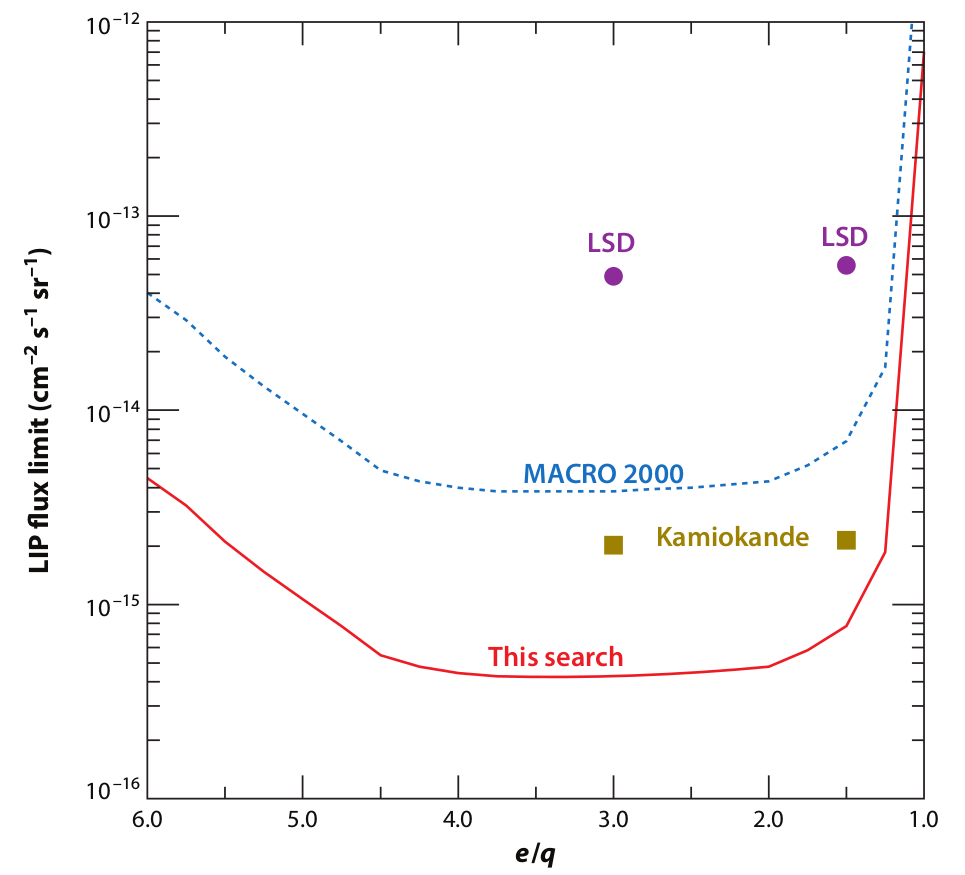
\includegraphics[width=0.7\textwidth]{chapter2/img/upperlimits_changed.png}
\caption{Upper limits on fluxes of particles close to the respective detectors. LIP stands for \textit{Lightly Ionizing Particles}. ``This search'' refers to an unpublished result from the MACRO experiment that compares the publised results from other experiments. Figure taken from Ref. \cite{Ambrosio:2004ub}, where I have changed the Kamiokande results which are wrong in the original figure.}
\label{fig:upperlimits}
\end{figure}

%https://arxiv.org/pdf/1601.04004.pdf +references!

\section{Properties of the signal}
\label{sec:properties}
Because there are many possible scenarios what these particles are, where they originate from, or how they are produced, one has to make certain assumptions about the properties of the signal. A particle traveling at the speed of light with a lifetime < 0.1 seconds traversing a detector will not give the same signal properties as one that has a very long lifetime. Therefore, I have assumed that the particles I am looking for
\vspace{2mm}

\begin{itemize}
\item behave leptonically, similar to muons. The particles will therefore produce long tracks instead of cascades in the IceCube detector (more info in Chapter \ref{ch:cherenkov});
\item have a long lifetime and will not rapidly decay within the IceCube detector, or at least have a very low probability to do so;
\item follow an energy spectrum with a spectral index of -2\footnote{More information about spectra can be found in Section \ref{subsec:whatarecosmicrays}.};
\item are assumed to produce an isotropic flux close to the detector.
\end{itemize}
\vspace{2mm}

\noindent These assumptions are consistent with previous searches that are mentioned in Section \ref{sec:prevsearches}. The behavior of such particles in the detector will depend on the charge (see Section \ref{subsub:energyloss}) and, to a lesser extent, the mass. In this work the particles are assumed to have a
\vspace{2mm}

\begin{itemize}
\item charge of 1/3, 1/2 or 2/3;
\item mass of 10 GeV, 100 GeV, 1 TeV, 10 TeV or 100 TeV,
\end{itemize}
\vspace{2mm}

\noindent where I have referred to the charge of the particles as relative to the absolute electron charge, $e$\footnote{This will be done throughout this work from this point on.}. The possible combinations result into a total of 15 unique signal samples that will be searched for.\\

\noindent The detector used in this analysis, the IceCube detector, is a neutrino telescope. The properties of the signal were defined to be able to compare this work to the results seen in Figure \ref{fig:upperlimits}. The best limits were set by the MACRO and Kamiokande experiments. The former was a multipurpose underground detector located at Gran Sasso, Italy and designed to search for magnetic monopoles with the use of liquid scintillators and streamer tubes \cite{Giacomelli:2007sk}. This design also made it possible to operate as a neutrino detector and cosmic ray observatory and allowed for BSM searches such as particles with a fractional charge.

The Kamiokande observatory, a water Cherenkov detector (see Chapter \ref{ch:cherenkov}) was designed to search for proton decay and located deep underground to shield the detector from cosmic ray muons (see Chapter \ref{ch:cr}). Because of its design and very efficient shielding from cosmic rays, the detector also operates as a neutrino observatory and can also be used to search for particles with a fractional charge. The experiment was later extended to Kamiokande II, III and Super-Kamiokande.  

%----------------------------------------------------------------------------------------
%	CHAPTER 3
%----------------------------------------------------------------------------------------
\chapterimage{cosmicrays-s.jpg} % Chapter heading image
\chapter{Cosmic Rays and Neutrinos}
Cosmic rays alsmost exclusively refer to particles with a finite rest mass. The term \textit{rays} was historically wrongly attributed to these particles as they were thought to be mostly electromagnetic radiation.
The interest of cosmic rays within the field of particle physics and modern particle physics is clear: multiple new particles were discovered from the interactions at energies which were higher than most experiments could reach. Positrons, muons, pions and kaons were first discovered in cosmic ray experiments in the 1930s and 40s. Today, high-energy cosmic ray interactions are still of interest as the highest energies of these particles go beyond what is feasible at the most powerful accelorators such as the LHC. Neutrinos are expected be produced toghether with cosmic rays near the source or close to Earth making neutrino astronomy a powerful and important part of modern day astronomy. In this chapter I will give BLA BLA BLA. For a more exhaustive description of cosmic rays I refer the reader to \cite{Gaisser:2016uoy}.

\section{Cosmic rays}
\subsection{Discovery of cosmic rays}
With the use of electrometers, Victor Hess performed multiple ground-breaking balloon flight experiments in 1912 to prove that the amount of radiation increases with altitude \cite{hessnobel:1936}. This was in strong contradiction with the widespread belief that radiation on Earth's surface mostly originates from radioactive substances in its crust. Hess concluded that an extremely penetrating radiation existed. He described this radiation to be coming from space wich then enters Earth's atmosphere which proved to be correct but it was wrongfully attributed to electromagnetic radiation by Robert Millikan in the 1920s \cite{PhysRev.32.533}. 

Hess later ruled out the possibility that cosmic rays originate from the Sun as his observations showed no particular differences in night and day and during solar eclipses. In the late 1920s, first evidence was found that cosmic rays were charged due to a variation of their intensity with latitude \cite{clay:1927a}. This indicated that they were deflected by the geomagnetic field.

\subsection{What are cosmic rays?}
\label{subsec:whatarecosmicrays}
Cosmic rays are, almost exclusively, the collection of nuclei which are stripped of their electrons, making them electrically charged, heavy particles. Around 90\% of the particles are ionized hydrogen atoms, or protons. 9\% are alpha particles and 1\% are nuclei of heavier elements. There is a striking resemblance between the relative abundance of cosmic rays and elements in the Solar System as seen in Fig. \ref{fig:relabundance}. A much smaller fraction of incoming particles are electrons, positron and antiprotons.

\begin{figure}
\label{fig:relabundance}
\centering
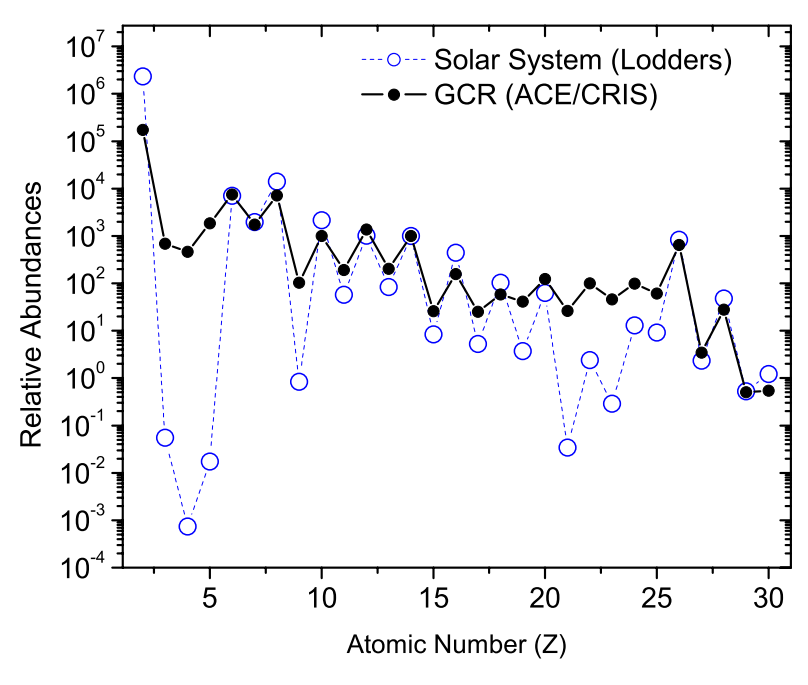
\includegraphics[width=0.7\textwidth]{./chapter3/img/relativeabundanceACE.png}
\caption{The cosmic ray elemental abundances measured on Earth compared to the solar system abundances, all relative to carbon = 100. Figure from ACE news archive \cite{ISRAEL2005201}.}
\end{figure}
There are however two important differences between cosmic rays and elements from our Solar System. Firstly, the two groups of elements Li, Be, B and Sc, Ti, V, Cr, Mn are many orders of magnitude more abundant in cosmic rays than in the solar system. This is due to their absence in stellar nucleosynthesis and are therefore not expected to be produced in large numbers. More massive cosmic rays (mainly C, O and Fe) can produce these nuclei in the process of \textit{spallation}. They are produced by collisions of cosmic rays with the interstellar medium. Therefore, these nuclei are sometimes referred to as \textit{secondary nuclei}.
The second difference is that nuclei with $Z>1$ are much more abundant with respect to hydrogen for cosmic rays. This phenomenon is not yet well understood but could be attributed to the difficulty to ionize hydrogen, necessary for acceleration processes.

The amount of cosmic rays seen on Earth is expressed in units of $\left[m^{-2} s^{-1} sr^{-1}\right]$. We can see in Fig. \ref{fig:spectrumCR} that the cosmic ray flux follows a energy power law spectrum:

\begin{equation}
\label{eq:spectrum}
dNdE \varpropto E^{-\gamma} dE,
\end{equation} 
where $\gamma$ is called the \textit{spectrum index}. Because of the steepness of the spectrum it is often multiplied by a higher power of energy\footnote{The broad range in both energy and flux should convince the reader that many types of detectors are necessary to study the behaviour of cosmic rays. Low-energy particles are abundant and high-energy particles are much more rare. Both the energy and the incoming flux will determine the type and size of the detector.}.

\begin{figure}
\label{fig:spectrumCR}
\centering
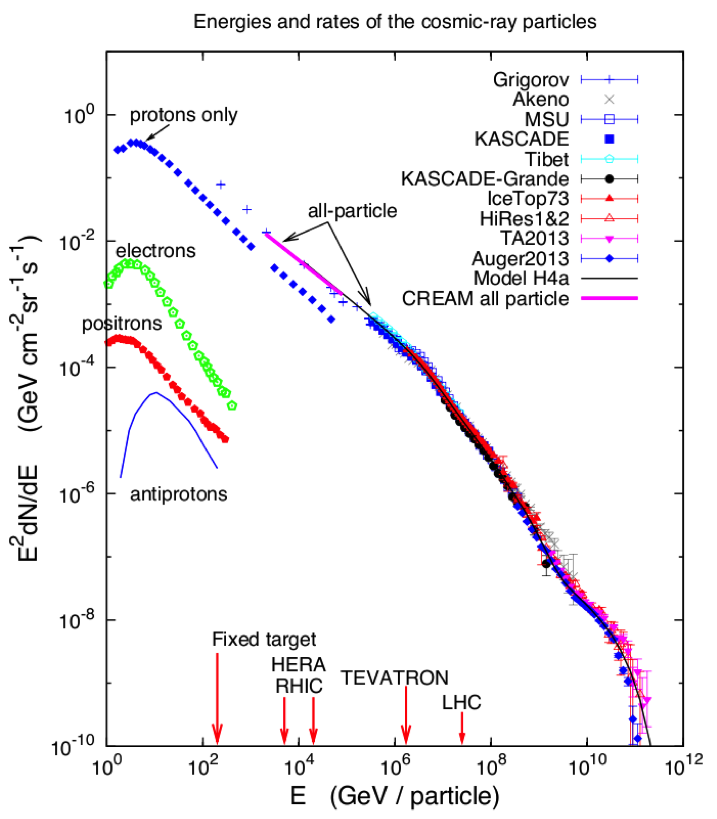
\includegraphics[width = 0.6\textwidth]{chapter3/img/spectrumCR.png}
\caption{Spectrum of cosmic rays at Earth. The all-particle spectrum measured by different experiments is plotted together with the proton-only spectrum. Subdominant contributions to the total flux from electrons, positrons and antiprotons as measured by the PAMELA experiment are also shown. Figure from \cite{Blasi:2013rva}.}
\end{figure}

We can divide the global spectrum in four regions. Between 10 GeV and 1 PeV the differential spectrum index is around -2.7. From 10 PeV to 1 EeV it is around -3.1. Above 10 EeV the spectrum again flattens to an index around -2.6 and an apparent cutoff region is present at around $10^{20}$ eV. The transition of this first to second region is referred to as the \textit{knee} at around 3 PeV. The second to third region transition is referred to as the \textit{ankle}. It is possible to describe the full cosmic-ray spectrum with sources within our galaxy. A more generally accepted theory is that the knee in the spectrum originates from the end of a population of particles which are accelerated within our Milky Way \cite{Gaisser:2013bla}. A sometimes referred to at around 100 PeV is the \textit{second knee}, believed to be a feature of the iron drop-off.
The origin of cosmic rays has been a topic of discussion for many years. We know now that most particles originate from sources in the local galaxy, having spent on average $10^7$ years in diffusive motion in the interstellar medium \cite{Gaisser:2013bla}. This is consistent with the resemblance of the relative abundances of cosmic rays and elements from our Solar System. However, there is no general consensus about the origin of the cosmic rays with energies above $3 \times 10^{18}$ eV. In the following, the abovementioned energy regions are discussed in more detail.

\subsubsection{Solar modulation}
In the Solar System a stream of charged particles is released from the Sun. This stream is mostly made up of electrons, protons and alpha particles with kinetic energies ranging between 0.5 and 10 keV. Within this solar wind plasma there is a magnetic field. Cosmic rays coming in to the Solar System interact with these particles and magnetic field. The influence is greatest on particles with the lowest charges. This effect is called \textit{solar modulation}. In effect, we see a strong suppression of cosmic rays at energies of 10 GeV and below.

\subsubsection{Galactic component}
The most probable acceleration mechanism for cosmic rays originating from our Galaxy is by shocks driven by expanding supernova remnants \cite{0034-4885-64-4-201}. From the ratio of primary to secondary nuclei it can be inferred that cosmic rays travel distances thousands of times greater than the thickness of the disk of the Galaxy. There is also an apparent decrease in the amount of matter that is traversed by cosmic rays with higher energies than with lower. Higher-energy cosmic rays seem to spend less time in the Galaxy than lower-energy ones and suggests that cosmic rays are accelerated before most propagation occurs \cite{Gaisser:2016uoy}.

The way the spectrum is fit is not set in stone. Here I will use the convention used by Gaisser, Stanev and Tilav described used in reference \cite{Gaisser:2013bla}. The spectrum is subdivided in three populations. The first population corresponds to the particles accelerated by supernova remnants, with the knee signaling the cutoff of this population. The second population is a higher-energy galactic component of unknown origin. The third generation will be described in more detail in \ref{subsec:ankle}. Assuming that the primary spectrum depends on the \textit{magnetic rigidity}\footnote{An assumption which is experimentally favored over other assumptions. Rigidity is an appropriate variable for interpreting changes in the spectrum due to propagation and acceleration in magnetic fields.},

\begin{equation}
R = \frac{pc}{Ze},
\end{equation}
where $Ze$ is the charge of a nucleus of total energy $E_{tot} = pc$ and relates to the gyroradius of a particle in a given magnetic field $B$ as

\begin{equation}
\label{eq:gyro}
r_L = \frac{R}{B}.
\end{equation}
If there is a characteristic regidity, $R_e$ above which a particular acceleration process reaches a limit, then the feature will show up in total energy first for protons, then for helium and so forth for heavier nuclei according to

\begin{equation}
E_{tot} = Ze \times R_e.
\end{equation}
This effect is visualised in Fig. \ref{fig:fitsgaisser} and indicates that as one population reaches its maximum the composition becomes heavier. The second knee, reported by KASCADE-Grande \cite{Apel:2011mi} and GAMMA \cite{Garyaka:2008gs} could be explained with an ``iron knee'' bump.

\begin{figure}
\label{fig:fitsgaisser}
\centering
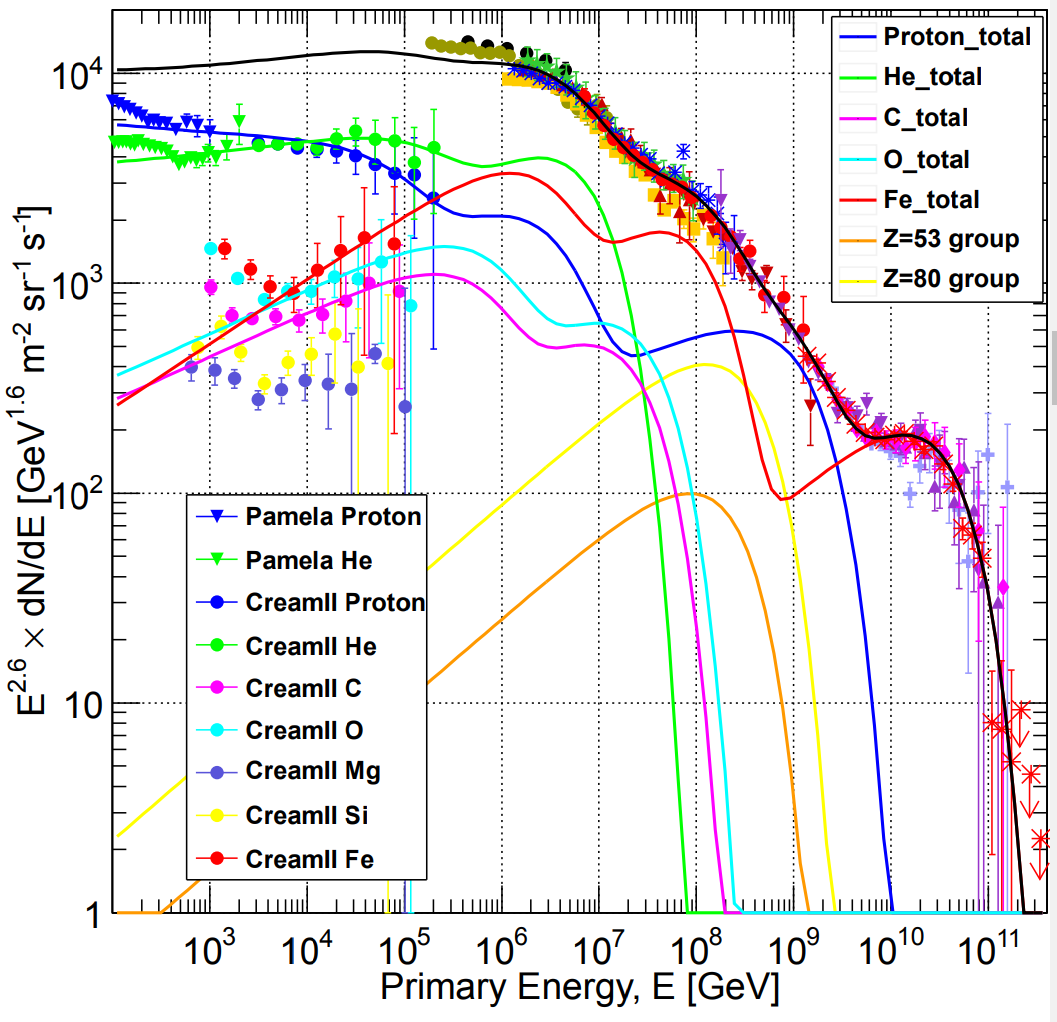
\includegraphics[width=0.48\textwidth]{chapter3/img/fit1gaisser.png}
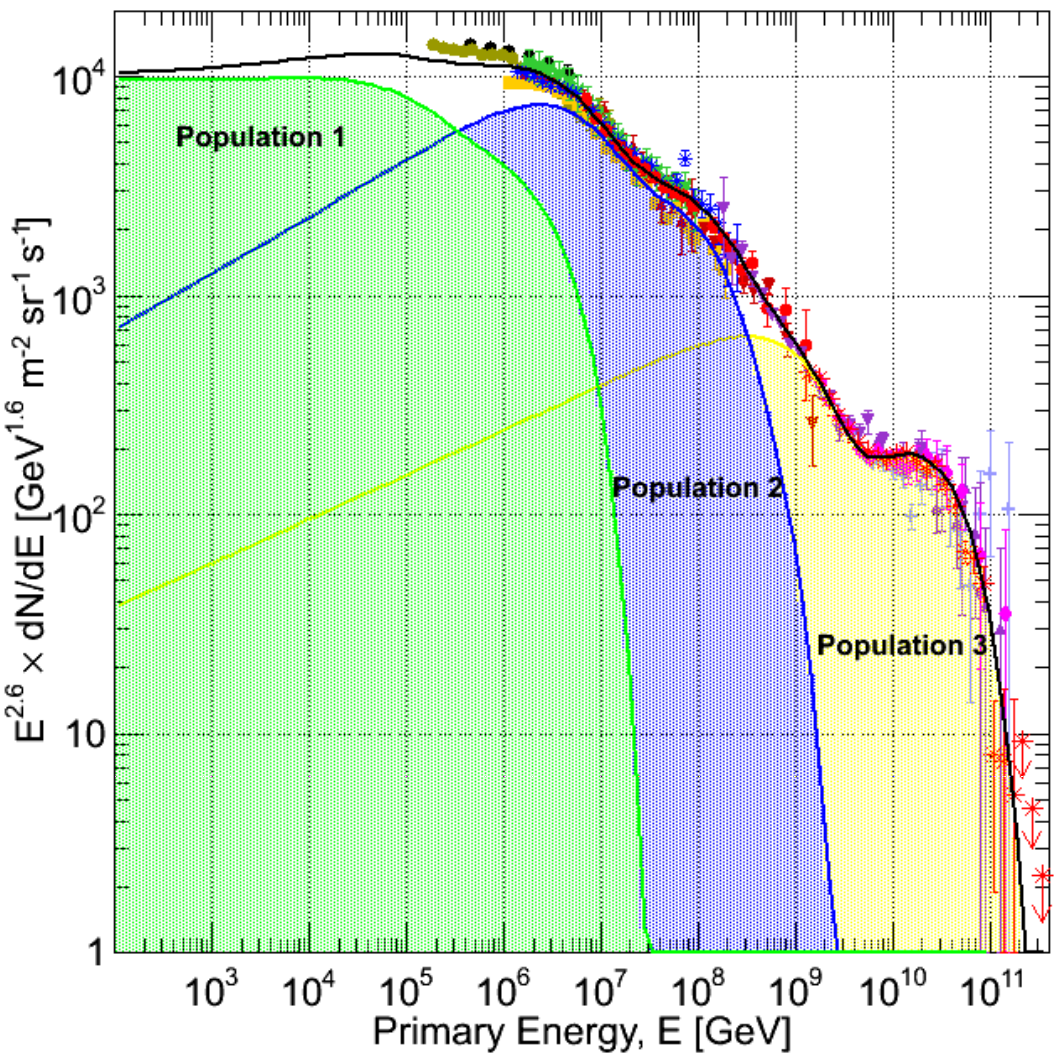
\includegraphics[width=0.48\textwidth]{chapter3/img/fit2gaisser.png}
\caption{Blub}
\end{figure}

%A schematic picture of our home galaxy, the Milky Way, is shown in Fig. 1.2. Most stars are concentrated in the galactic disc of height h $\approx$ 300 pc in the form of spiral arms. The disc is filled with warm atomic gas that consists to 90\% of H and to 10\% of He and has an average density n approx 1/cm3. It contains also an ordered magnetic field with strength B approx 3microG. The energy when the Larmor radius
\subsubsection{Extragalactic component}
The flux at the highest energies is exceedingly small. The number of events per year at energies above $5 \times 10^{19}$ eV is around one per square kilometer per century. There are only two experiments in the world capable of detecting the highest-energy cosmic rays in a statistical meaningful way: Telescope Array, located in the Northern Hemisphere (area of $\approx$700 km$^2$) and the Pierre Auger Observatory in the Southern Hemisphere (area of $\approx$3000 km$^2$).

Both experiments see a suppression of the flux above $6 \times 10^{19}$ eV. The exponential cutoff is consistent with the expected Greisen-Zatsepin-Kuzmin (GZK) effect \cite{Greisen:1966jv,Zatsepin:1966jv} where cosmic rays interact with the cosmic microwave background radiation (CMB)

\begin{equation}
\gamma_{CMB} + p \rightarrow \Delta^+ \rightarrow p + \pi^0
\end{equation} 
or

\begin{equation}
\gamma_{CMB} + p \rightarrow \Delta^+ \rightarrow n + \pi^+.
\end{equation}
Particles with energies above $5 \times 10^{19}$ eV would interact with the CMB, leading to an exponential cutoff (but if the incoming particles above these energies would be relatively young it is still possible for them to reach the detector). The Pierre Auger experiment reported to see higher compositions at the highest energies \cite{icrc2017:pa}. If the particle is a nucleus with A nucleons, then the GZK limit applies to its nucleons, which carry only a fraction 1/A of the total energy. For iron nuclei this would for example result in a limit of $2.8 \times 10^{21}$ eV. In contrast, the TA experiment interpreted their data as implying a light primary composition (mainly p and He) at the highest energies. Both experiments use a different interpretations for crucial quantities of these measurements and a thorough join analysis conducted by both experiments states that, at the current level of statistics and understanding of systematics, both data sets are compatible with being drawn from the same parent distribution \cite{PDG2018url}.

\begin{figure}
\label{fig:ankle}
\centering
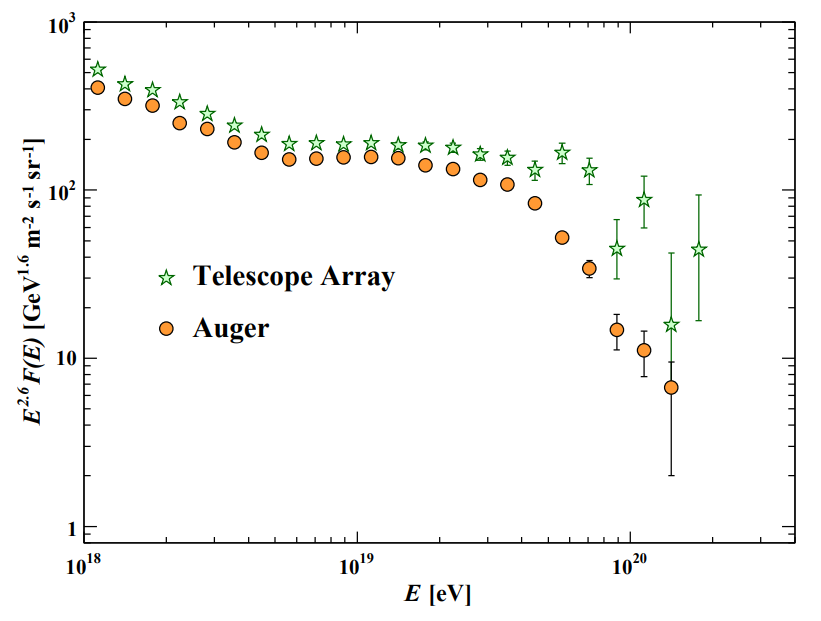
\includegraphics[width=0.6\textwidth]{chapter3/img/ankle.png}
\caption{Expanded view of the higest energy portion of the cosmic-ray spectrum from data of the Telescope Array and the Pierre Auger Observatory \cite{pdg2018}.}
\end{figure}
The Pierre Auger Observatory also reported evidence in an anisotripic distribution of the arrival directions of the highest-energy cosmic rays \cite{Aab:2017tyv} in a direction where the distribution of galaxies is relatively high and does not coincide with the galactic plane. These observations, together with our lack of known possible sources within our galaxy for these ultra-high energies shows compelling evidence that these particles have an origin from outside our galaxy. From pion decay there is also an expected flux from extragalactic neutrinos (more information in section \ref{subsec:astro} and \ref{waarjehetinhoofdstuk5gaatbespreken}). The flux, spectrum and angular distribution of the excess neutrino signal detected by IceCube between $\approx 50$ TeV and $\approx 2$ PeV are inconsistent with those expected for Galactic sources \cite{Waxman:2013zda}.\\
\newline
To put it simply, understanding cosmic rays and where they originate can help us answer fundamental questions about the origins of the universe, our galaxy and ourselves. To put it in the words of Carl Sagan:

\begin{center}
\begin{minipage}[5cm]{0.9\textwidth}
\textit{``The nitrogen in our DNA, the calcium in our teeth, the iron in our blood, the carbon in our apple pies were made in the interiors of collapsing stars. We are made of starstuff.''}
\end{minipage}
\end{center}

\subsection{Acceleration mechanism}
How cosmic rays got their signature slope in the energy spectrum and its intricate details have been under discussion for multiple decades. To this date there is no clear picture how these particles are accelerated in full detail. It is beyond the scope of this work to give a comprehensive overview of all possible acceleration mechanisms or possible sources. Most calculations are left out and for a more detailed discussion the reader is referred to specialized books or the references in the text.\\
\newline
The acceleration of the particles can be subdivided into two questions. First, where are the particles accelerated? Does it happen on large scales, cosmological distances in galaxies or near specific sources? Secondly, how are these particles exactly accelerated? What is the driving mechanism? Since primary cosmic rays are all electromagnetically charged particles these mechanisms should clearly be sought for in places where electric and/or magnetic fields play a dominant role.

\subsubsection{Galactic accelerators}
With their approximate energy density around 0.5 eV/cm$^3$ in our local galaxy, the bulk of cosmic ray acceleration could very well be explained by \textbf{supernovae}. This density results into a total power of around

\begin{equation}
L_{CR} = 7 \times 10^{40} \textrm{ erg/s},
\end{equation}
where erg is a unit often used in astonomy\footnote{1 erg = $10^{-7}$ J.}. If one assumes a supernova explosion of around one per every 30 years then the total power output of type II supernovae with a mass output of around ten times the mass of the Sun at a velocity close to $5 \times 10^{8}$ cm/s would result in a power of

\begin{equation}
L_{SN} \backsim 3 \times 10^{42} \textrm{ erg/s}.
\end{equation}
These numbers are not set in stone and hold large uncertainties, but it shows that with an acceleration efficiency on the order of a couple of percent supernova explosions are a prominent source of energetic cosmic rays, if not the dominant one.

\subsubsection{Extragalactic accelerators}
We will see in Section \ref{para:maxenergy} that the maximum energy from shock acceleration by a supernova remnant is insufficient to explain UHECR. As explained in Section \ref{para:fermiacceleration}, particles can be accelerated if the trajectory of the particles can be changed and energy can be transferred multiple times. The magnetic fields responsible for the course change of these particles has to be sufficient in magnitude in order for these particles not to escape and go beyond the grasp of the source responsible for the acceleration. This limitation is expressed by the gyroradius in the accelerator, $r_L = E/ZeB$ similar to Eq. \ref{eq:gyro}, requiring it to be smaller than the radius of the accelerator: $r_L < R$ or $E < ZeBR$.

Even if only qualitative, this relation provides an interesting criterion to idendify possible sources of UHECRs by looking at the accelerator related term $BR$. This was done in a classic paper by Hillas \cite{Hillas:1985is}, illustrated in the more recent Fig. \ref{fig:hillas}. Accelerators necessary to explain the amount of UHECRs are not populated (enough) in our galaxy, making them more likely to be of extra-galactic origin. \textbf{Active galactic nuclei, blazars and gamma ray bursts} (en andere als je die hebt toegevoegd later) are therefore also briefly explained.

\begin{figure}
\label{fig:hillas}
\centering
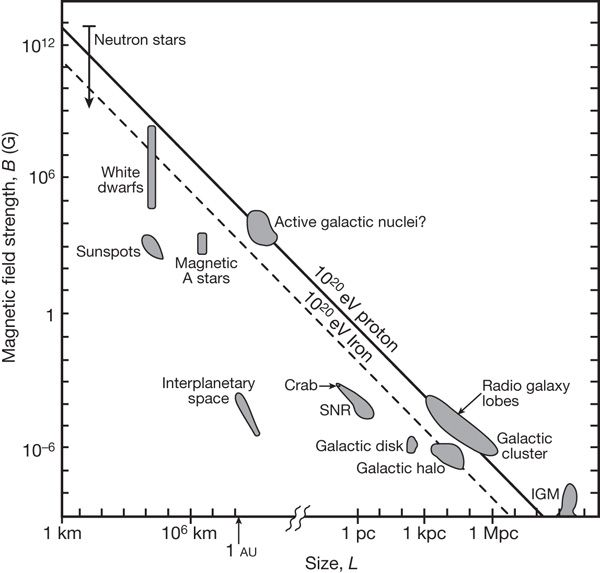
\includegraphics[width = 0.7\textwidth]{chapter3/img/Hillas.jpg}
\caption{The Hillas plot of potential cosmic ray accelerotors locates objects according to size and magnetic field. Objects to the left of the diagonal lines cannot accelerate particles to $10^{20}$ eV (proton: solid, iron: broken). Image obtained from HIER "REF" TOEVOEGEN, OVERAL EIGENLIJK \cite{Bauleo:2009zz}}
\end{figure}



\subsection{Sources}
\subsubsection{Supernova (remnants)}
Supernovae can be broadly subdivided into two categories: type I and type II. Type I supernova explosions happen in binary star systems. In those systems one of the two starts is a carbon-oxygen white dwarf which accretes matter from the second star. When the total mass of the white dwarf reaches the Chandrasekhar REF limit of around 1.44 solar masses it cannot longer hold itself under the gravitational pressure and collapses in on itself. Within seconds, the carbon component in the white dwarf starts nuclear fusion and enough energy is released to produce an explosion brighter than the Sun with a factor of around 5 billion. 
A resulting shock wave can reach up to around 3\% the speed of light.

Type II supernova explosions differ by being single star systems. When a star reaches the end of its lifecycle the subsequent fusion reactions reach to a halt. If the star has enough mass (at least 8 times the mass of the Sun), it is possible for the inner core to again reach the Chandrasekhar limit and collapse in on itself due to the lack of \textit{electron degeneracy}. Without the outward pressure of nuclear fusion reactions and the support of the core, the outer layers of the star collapse under the gravitational pressure. The compression of the electrons and protons into neutrons results into a very hot, dense, neutron core. The velocity of the inwards falling layers can reach to a staggering 23\% of the speed of light and recoil when hitting the remaining core. Neutrinos are produced in this violent core collapse and the outward going shockwave hits the remaining outer layers forming the supernova explosion \footnote{Astronomer Carl Sagan once said, "The nitrogen in our DNA, the calcium in our teeth, the iron in our blood, the carbon in our apple pies were made in the interiors of collapsing stars. We are made of starstuff."}.

Because of their brightness supernovae within our galaxy can be seen with the naked eye (provided they are not too far away). The last recorded supernova from our galaxy was by Johannes Kepler in 1604 but earliest recordings go back to 185 AD by Chinese astronomers\footnote{From observations of other galaxies supernovae are expected to occur, on average, once every thirty years. Not all of these will be visible to the naked eye, but would almost certainly be observable with modern astronomical telescopes.}.
\begin{figure}
\label{fig:supernova}
\centering
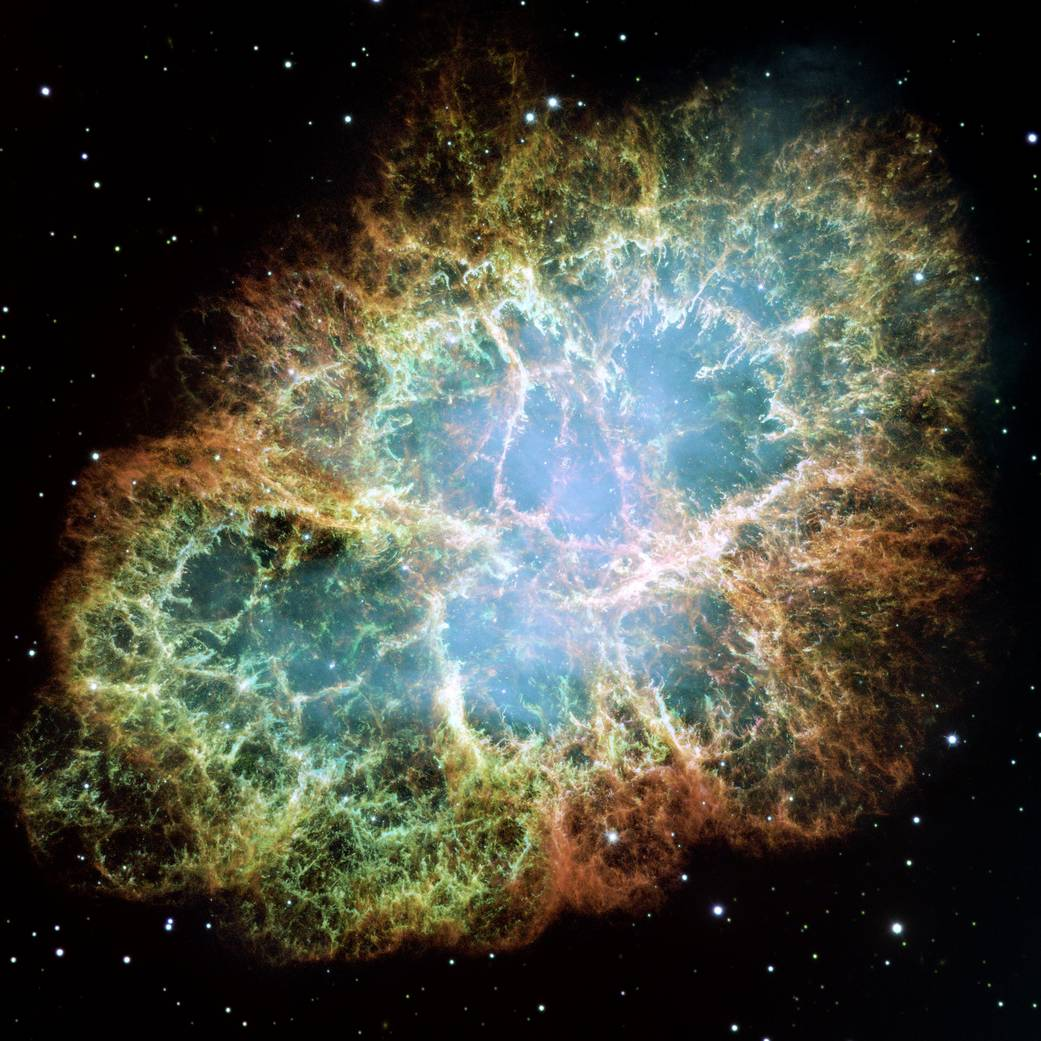
\includegraphics[width=0.48\textwidth,height=8cm]{chapter3/img/crabnebula.jpg}
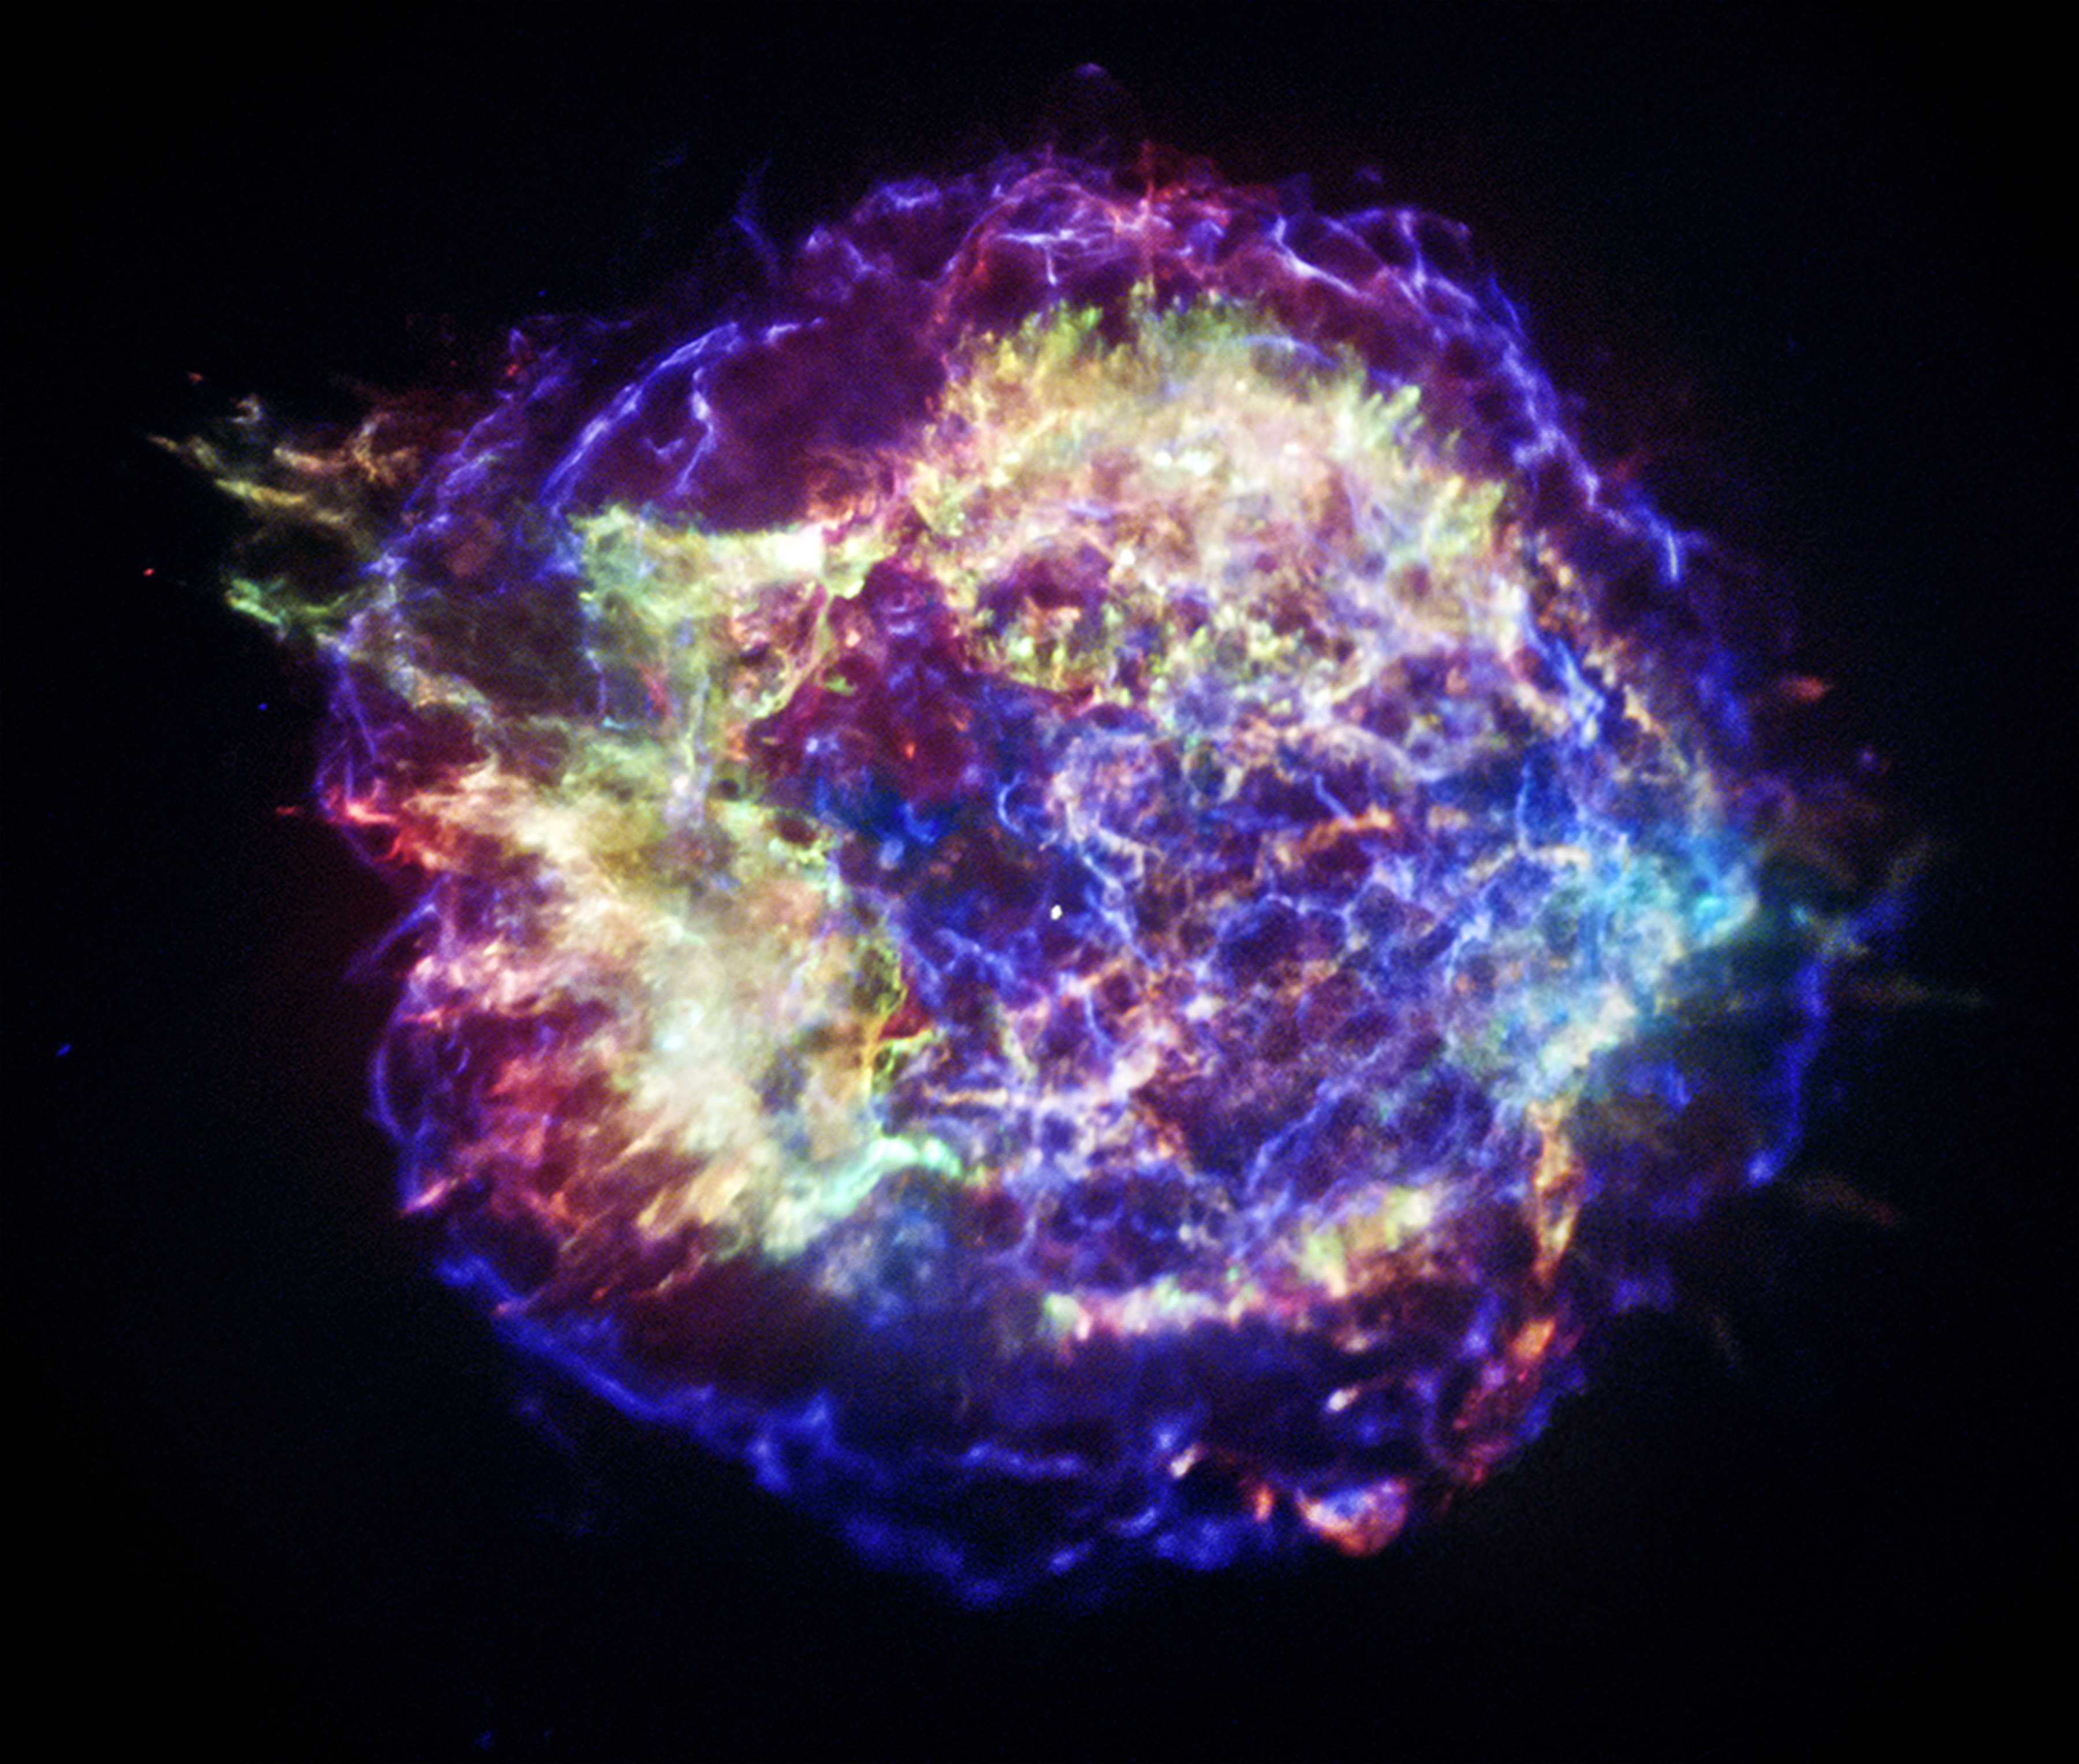
\includegraphics[width=0.48\textwidth,height=8cm]{chapter3/img/casa.jpg}
\caption{Left: the Crab Nebula is the supernova remnant approximately one thousand years old. The supernova was noted by Chinese astronomers in the year 1054 AD. Right: Chandra X-ray observatory picture of the Cassiopeia A supernova remnant (pictures from NASA).}
\end{figure}
\newline
The question remains how supernovae can serve as cosmic ray accelerators. In 1949, Enrico fermi proposed a mechanism where particles can gain energy by collisions with moving interstellar ionized gas clouds. Only later, it was realized that a large, plane shock front moving with a certain velocity is able to accelerated charged particles much more efficiently. This first mechanism results into an energy transfer proportional to the squared velocity of the cloud and is thus called \textit{second order Fermi acceleration}. Shock front acceleration energy transfer is proportional to the velocity and is called \textit{first order Fermi acceleration}. Supernova remnants provide an explanation for the origin of these shock fronts.

\paragraph{First- and second-order Fermi acceleration}
\label{para:fermiacceleration}

Suppose we have a magnetic cloud in the interstellar medium travelling with a certain velocity $\vec{V}$ and a particle with velocity $\vec{v}$ enters the cloud under an angle $\theta_1$ (see Fig. \ref{fig:cloud}). If we assume collisionless scattering can occur (no energy is dissipated from the particle to the cloud) due to the magnetic fields in the cloud, the magnitude of the momentum in the rest frame of the cloud will not change ($E'_1 = E'_2$, where we the apostrophe denotes the cloud rest frame). From special relativity we know that:

\begin{figure}
\label{fig:cloud}
\centering
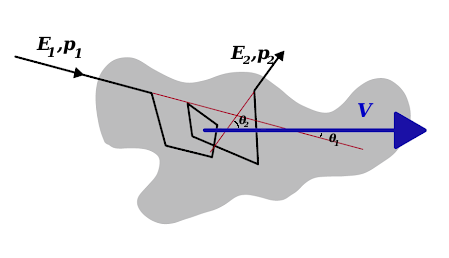
\includegraphics[width=0.48\textwidth]{chapter3/img/cloud.png}
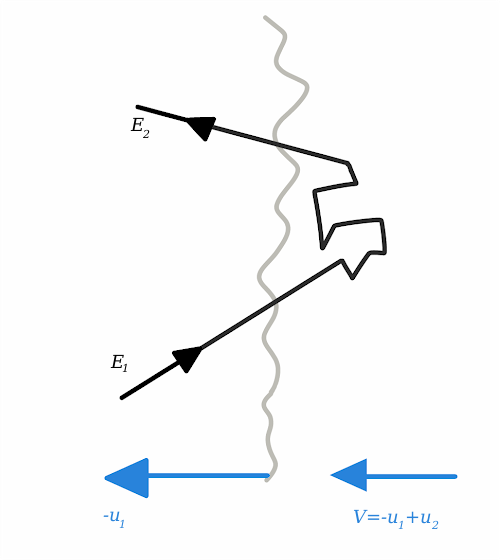
\includegraphics[width=0.48\textwidth]{chapter3/img/shock.png}
\caption{Left: magnetic cloud. Right: shock waves typically have magnetic inhomogeneities both preceding (downstream) and following them (upstream). If a charged particles travels trough the shock wave it can gain velocity through first-order Fermi acceleration. In the illustration a particle travels from upstream to downstream and back upstream. At every back and forth movement the particle effectively gains in energy. For a particle with a velocity $u_1$ relative to the shock front the front seems to come at him with velocity $-u_1$. The downstream medium has a velocity relative to the shock front of $u_2 < u_)1$ making it seem coming towards the particle with velocity $u_1-u2$.}
\end{figure}

\begin{equation}
\begin{split}
E'_1 &= \gamma \left(E_1 - p_{1,\parallel} V\right) \\
&= \gamma E_1 \left(1-\beta \cos \theta_1\right),
\end{split}
\end{equation}
with $\beta = V/c$ and $\gamma$ the Lorentz factor. Similarly and using $E'_1 = E'_2$

\begin{equation}
\begin{split}
E_2 &= \gamma E'_2 \left(1+\beta \cos \theta_2'\right)\\
&=\gamma^2 E_1 \left(1-\beta \cos \theta_1\right) \left( 1 + \beta \cos \theta_2'\right)
\end{split}
\end{equation}
and

\begin{equation}
\frac{\Delta E}{E} = \frac{E_2 -E_1}{E_1} = \frac{1 - 
\beta \cos \theta_1 + \beta \cos \theta_2' - \beta^2 \cos \theta_1 \cos \theta_2'}{1-\beta^2} -1.
\end{equation}
By hypothesis, the escaping particles are isotropic in the cloud frame: $\langle \cos \theta_2' \rangle = 0$. One can show that $\langle \cos \theta_1 \rangle = -\frac{\beta}{3}$ \cite{Gaisser:2016uoy}, leading to

\begin{equation}
\frac{\Delta E}{E} = \frac{4}{3} \frac{\beta^2}{1-\beta^2} \approx \frac{4}{3} \beta^2,
\end{equation}
showing that for molecular clouds the energy gain is indeed proportional to the square of $\beta$ for second-order Fermi acceleration.\\
\newline
If a particle is incoming to an expanding shock (see Fig. \ref{fig:cloud}) $\langle \cos \theta_2'\rangle$ is equal to 2/3, leading to

\begin{equation}
\frac{\Delta E}{E} = \frac{\frac{4}{3}\beta + \frac{13}{9}\beta^2}{1-\beta^2} \approx \frac{4}{3} \beta,
\end{equation}
where $\beta$ is now equal to $u_1 -u_2$ as explained in the caption of the figure. We have shown that for shock fronts the energy gain is indeed proportional to $\beta$ for first-order Fermi acceleration. From both the outcome as the discussion it is clear that the energy gain enters through relativistic effects, making the intuitive approach not straightforward.

\paragraph{Power}
\label{para:power}
The energy gain of a ``single collision'' results into the power law spectrum when considering a process in which a test particle increases its energy by an amount proportional to its energy wich each encounter. Let us assume $\Delta E = \xi E$, after $n$ encounters:

\begin{equation}
E_n = E_0 \left(1+\xi\right)^n,
\end{equation}
where $E_0$ is the energy when the particle first enters the accelerator medium. To reach a certain energy $E'$, the particles must encounter a number of collisions

\begin{equation}
\label{eq:n}
n(E') = \frac{\ln \left(\frac{E'}{E_0}\right)}{\ln \left(1+\xi \right)}.
\end{equation}
To reach energies of $E'$ or higher, the number of collisions will be proportional to

\begin{equation}
\begin{split}
N(\geq E') \varpropto &\sum^\infty_{m=n} P_{present}(m) = \sum^\infty_{m=n} \left(1-P_{esc} \right)^m\\
&= (1-P_{esc})^n \left((1 - P_{esc}) + (1 - P_{esc})^2 + ...\right) \\
&= \frac{(1-P_{esc})^n}{P_{esc}},
\end{split}
\end{equation}
where $P_{present}$ is the probability of a particle still being present in the accelerator and $P_{esc}$ the probability of the particle to escape after per collision. Making use of $a^{\ln b} = e^{\ln a \ln b} = b^{\ln a}$ and inserting Eq. \ref{eq:n}

\begin{equation}
N(\geq E') \varpropto \frac{1}{P_{esc}} \left(\frac{E'}{E_0}\right)^{-\gamma},
\end{equation}
with

\begin{equation}
\gamma = \frac{\ln \left(\frac{1}{1-P_{esc}}\right)}{\ln \left(1 + \xi \right)} \approx \frac{P_{esc}}{\xi}.
\end{equation}
The power law spectrum becomes visible in the derivative of the number of particles in energy

\begin{equation}
\frac{dN}{dE} \backsim E^{-(\gamma + 1)},
\end{equation}
in agreement with Eq. \ref{eq:spectrum}. Shock wave fronts have an expected $\gamma \approx 1$ giving rise to a different spectrum to what is seen on Earth but which can be explained by propagation from the source to Earth (this is beyond the scope of this work). The spectrum from Fermi shock acceleration is thus expected to follow an $E^{-2}$ powerlaw behaviour.\\
\newline
Seems plausible all galactic CRs are accounted for my supernovae. This is supported with the realization that first-order Fermi acceleration naturally produces a spectrum of cosmic rays close to what is observed.

\paragraph{Maximum energy}
\label{para:maxenergy}
The highest energies that particle can be accelerated to can be defined by:

\begin{itemize}
\item The differential energy gain per collision $dE/dt$
\item The total time the particle can be accelerated
\end{itemize}.
The energy gain is given by
\begin{equation}
\frac{dE}{dt} = \frac{\xi E}{T_{cycle}},
\end{equation}
where $T_{cycle}$ is the charactersitic time for one acceleration cycle. $T_{cycle}$ depends on the diffusion coefficients and velocities of the upstream and downstream regions and is set to $T_{cycle} \geq 20 E/(3 u_1 Z e B)$ by Lagage and Cesarsky \cite{Lagage:1983zz} for a strong shock and arguing that the diffusion lenth, $\lambda_D$ cannot be smaller than the Larmor radius of the parcticle. Particles with a Larmor radius greater than the irregularities holding a magnetic field are not prone to be heavily influenced by them. Lagage and Cesarsky therefore concluded that

\begin{equation}
E_{max} \leq \frac{3}{20} \frac{u_1}{c} Z e B (u_1 T_{ST}),
\end{equation}
where $T_{ST}$ is the Sedov-Taylor time where particles are less prone to escape and is $\backsim 1000 years$. For $u_1 \backsim 10^9$ cm/s \cite{stanev2010high}  and $B \backsim 3\mu G$ the Lagage and Cesarsky limit reads

\begin{equation}
E_{max} \leq Z \times 2.4 \times 10^5 GeV.
\end{equation}

\subsubsection{Active Galactic Nuclei}
Active Galactiv Neuclei (AGNs) are no stars at the end of their life cycle but active black holes located in the center of galaxies. In most older galaxies the stars at the center have reached the end of life and have gone supernova leaving behind white dwarfs or black holes. It is believed that most massive galaxies have supermassive black holes in their centers by the accretion of matter from surrounding large gas clouds \cite{Urry:1995mg,Antonucci:1993sg}. Their masses in current models range from $10^6$ to $10^{10}$ Solar masses \cite{Kazanas:2012sk}.

The efficient conversion from gravitational potential energy to kinetic energy and radiation make AGNs the most luminous persistent sources of electromagnetic radiation in the universe, and as such vergy good means in discovering distant objects. The accretion discs heat up due to the inward falling and produce light peaking in the ultraviolet waveband. Certain emission lines are also expected due to the radiation from excited cold atomic material. Some accretion discs produce jets which point opposite each other and their direction is defined by either the spin of the black hole, the accretion disc or a combination of both.  The most powerful AGNs are classified as \textit{quazars} and AGNs with a jet pointing toward the Earth is called a \textit{blazar}.

\begin{figure}
\centering
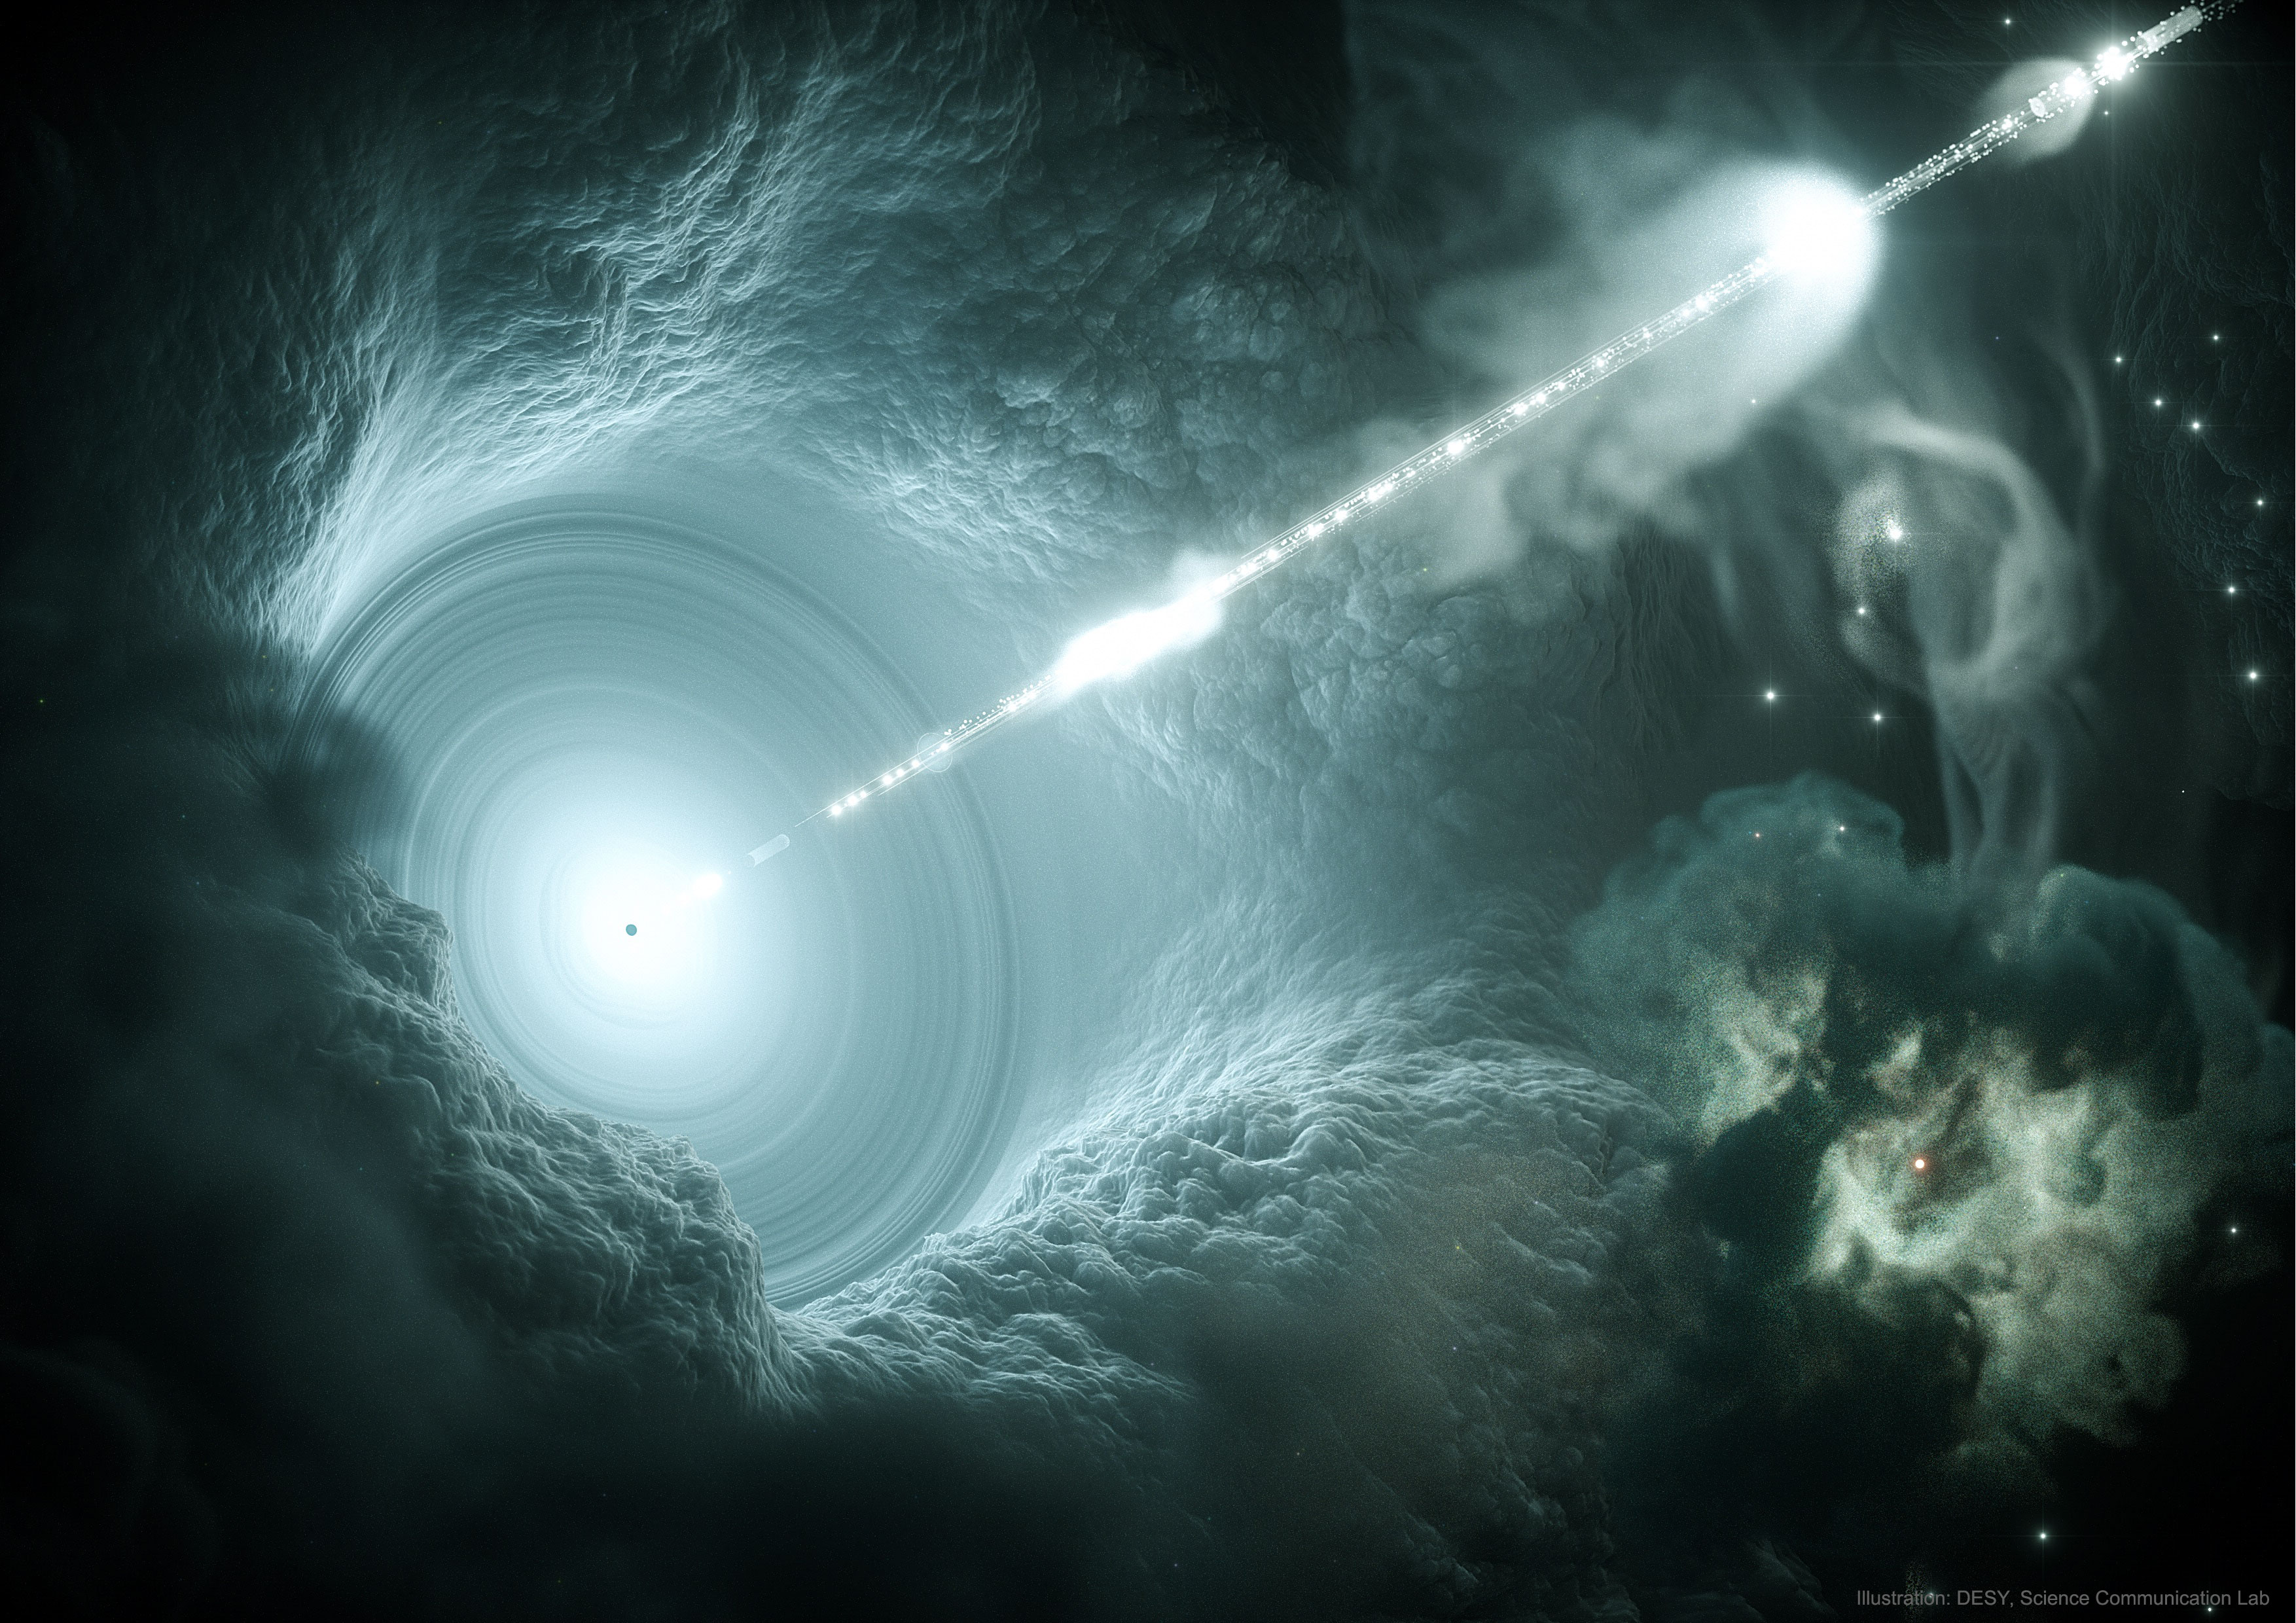
\includegraphics[width=0.49\textwidth]{chapter3/img/quazar.jpg}
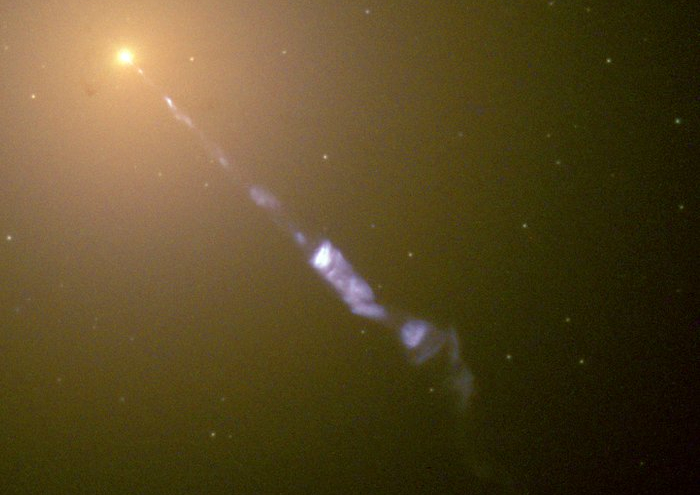
\includegraphics[width=0.49\textwidth]{chapter3/img/jet_crop.jpg}
\caption{Left: artist impression of a blazar which is recently been linked to a possible origin of extragalactic neutrinos \cite{TXS}. Illustration from DESY, Science Communication Lab. Right: Image from the Hubble telescope where we see a jet streaming out from the center of galaxy M87.}
\end{figure}

Charged partices have large cyclotron radii in AGNs and the relativistic jets could provide the necessary mechanisms to accelerate particles to ultra-high energies. Pierre Auger hinted to a correlation of the highest-energy cosmic rays with the positions of nearby active galactic nuclei \cite{Abraham:2007si}. Recently, a collaborative effort of IceCube, Fermi-LAT, MAGIC and others observed a coincidence of high-energy neutrinos and a blazar making them very good candidates of sources of extragalactic neutrinos \cite{IceCube:2018dnn}.

Misschien nog net iets meer uitwerken hoe UHECRs hier uit kunnen komen?
\subsubsection{Gamma Ray Bursts}
The most catastrophic deaths of massive stars or mergers of neutron-neutron stars or a neutron star and a black hole result into Gamma Ray Bursts (GRBs). GRBs are named after the burst of gamma rays that is followed by a longer-lived afterglow of electromagnetic radiation at longer wavelengths. These bursts are the most energetic explosions in the electromagnetic spectrum and occur when a high-mass star collapses to form a neutron star or black hole. A typical burst releases as much energy in a few seconds than the Sun will do in it's entire 10 billion-year lifetime and temporarily outshines the rest of the galaxy\footnote{GRBs were first discovered in the late 1960s by accident. The Vela sattelites had additional gamma ray detectors designed to detect very fast busts of gamma rays which are expected to be produced by nuclear tests in space \cite{Klebesadel:1973iq}}. GRBs are isotropically distributed, making them extragalactic in origin \cite{Meegan:1992xg}.

An often used model to explain how charged particles could reach extremely high energies is called the \textit{fireball model}. This internal-external shock model assumes that kinetic energy of an ultra-relativistic flow is dissipated in internal collisions. When the shock hits the surrounding matter it is slowed down and gives rise to the signature afterglow \cite{Piran:2004ba}. After initial the initial progenitor phase (see below) a plasma of photons, electrons, positrons and baryons develops into the formed jets. In this initial phase, the fireball is radiation-dominated and optically thick for photons, making it invisible in the electromagnetic spectrum. Due to radiative pressure the fireball expands at relativistic speeds ($\gamma$-factors $>$ 100) to the point that it becomes more and more transparent. If the central engine produces multiple shocks with different velocities there will be internal shocks, which give rise to the observed burst emission. In this mechanism, the ultra-relativistic matter can transfer it's kinetic energy to the acceleration of particles, explaining cosmic ray production. Later shocks of the jets with surrounding matter would explain the signature afterglow seen in GRBs.

Although there is still much ongoing discussion, GRBs are sometimes subdivided into two regions: \textit{long gamma ray bursts} ($t_{burst} > 2$s) and \textit{short gamma ray bursts} ($t_{burst} < 2s$). Long bursts originate from collapsars: a massive star core-collapse forms a black hole and surrounding matter is pulled into an accretion disk. Short burts hint to progenitors that are extremely compact, where neutron-neutron star or neutron star and black hole mergers are the most probable explanation. The recent detection of the gravitational waves can provide a significant contribution to the understanding of these sources \cite{TheLIGOScientific:2017qsa,Abbott:2017oio,Abbott:2017gyy,Abbott:2017vtc,Abbott:2016nmj}.

\begin{figure}
\centering
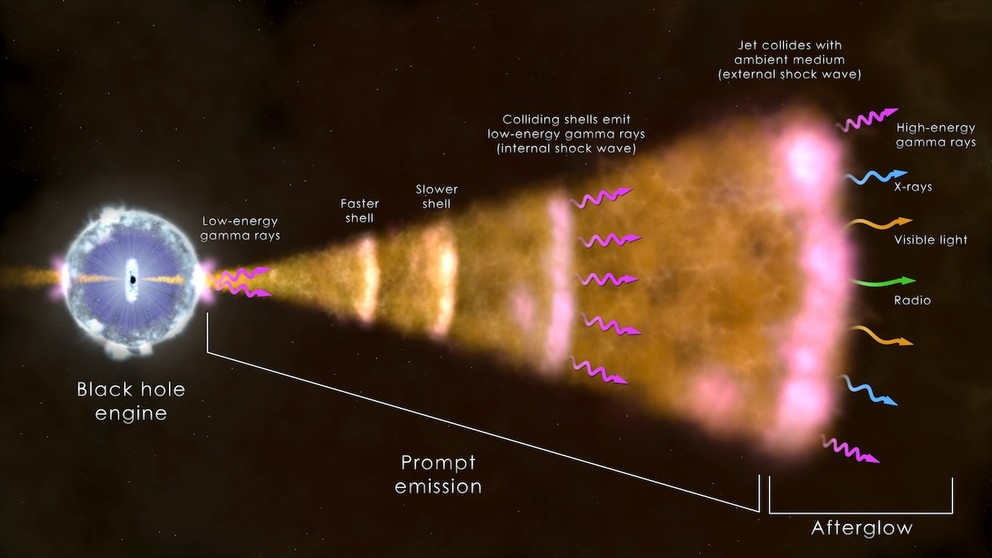
\includegraphics[width=0.6\textwidth]{chapter3/img/fireball.jpg}
\caption{In the fireball model ..... Image from NASA Goddard space flight center.}
\end{figure}

\subsubsection{Starburst galaxies}
Galaxies that undergo an episode of large-scale star formation, are called \textit{starburst galaxies}. Most of these are in the midst of a merger close encounter with another galaxy. Several experiments have shown their gamma ray emission at several hunderd GeV to be two to three orders of magnitude of that in our own Galaxy \cite{Acero:2009nb,Karlsson:2009hd}. Galactic scale winds from the central regions are possible sources for cosmic ray acceleration.

\subsubsection{Galaxy clusters}
When galaxies are bound togheter by gravity they are referred to as \textit{galaxy clusters}. They can contain around 100 to 1000 galaxies and have typical mass ranges around $10^{14}-10^{15}$ Solar masses. Through merging and accretion of dark matter and baryonic gas, galaxy clusters are expected to generate powerful shock waves on large scales. Shocks with significant velocities could provide the necessary conditions for cosmic ray acceleration \cite{•1538-4357-689-2-L105}.

\subsection{Propagation}
Doen of niet?

\section{Air showers}
\label{sec:airshowers}
When primary cosmic ray particles hit the Earth's atmosphere they give rise to a large shower of secondary particles. At low- to mid-energy ranges the abundance of cosmic rays is large enough for these showers to be analyzed with balloon or satellite experiments. As indicated in section \ref{subsec:whatarecosmicrays}, the flux of high-energy cosmic rays is so small, there is a need for very large-scale detectors, measuring kilometers in instrumented area.\\
\newline
The interaction length of nuclei with high energies is too small for them to be able to further than tens of kilometers in height. They will interact with an atmospheric nucleus and produce secondary particles. These particles, on their turn, decay or further interact with the atmosphere and give rise to an \textit{extensive air shower} if the production of new particles is large enough. Some of these particles will be stopped, but others are capable of reaching the Earth or even penetrate deep inside it. Although air showers are of significant importance in cosmic ray studies, we will only give a brief summary of the most noteworthy features and it's main importance for this analysis.
An air shower has three components: the hadronic, muonic and electromagnetic. The hadronic component can be seen as the core of the shower consisting of high-energy hadrons. The interactions and subsequent decays of these hadrons fuel the electromagnetic and muonic parts. A schematic overview is given in Fig. \ref{fig:airshower}. If the primary particle is a photon the shower is made up almost exclusively of an electromagnetic component. Because the lateral size of an electromagnetic cascade is caused by multiple scattering of electrons and positrons the lateral size of these showers is relatively small (radius around 1 km for a transversely downgoing 100 TeV photon). In hadronic cascades, on the other hand, the lateral size is caused by the transverse momenta of the secondary particles making these showers much larger (radius arond 4km for a transversely downgoing 100 TeV proton) \cite{Grupen:2005rx}.

\begin{figure}
\label{fig:airshower}
\centering
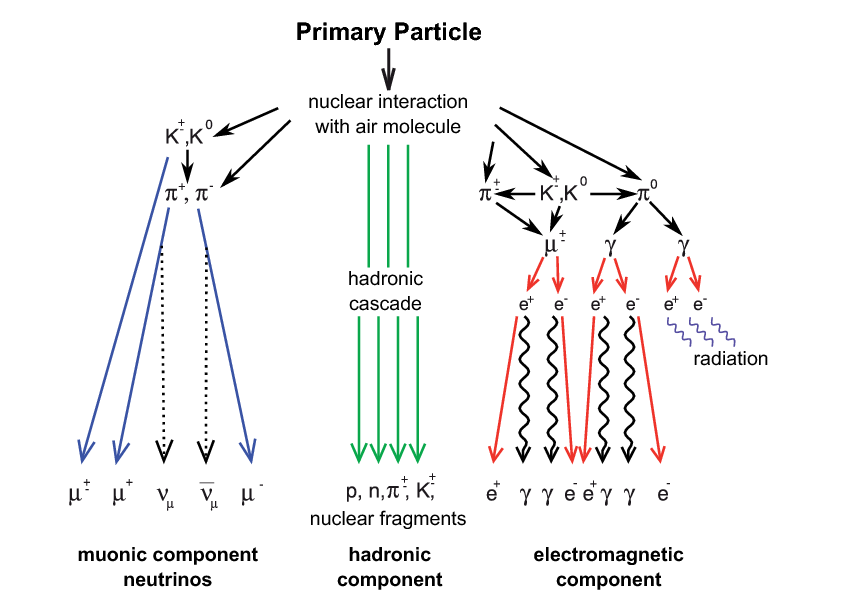
\includegraphics[width=0.8\textwidth]{chapter3/img/airshower.png}
\caption{Schematic view of an extensive air shower with a clear distinction between the three components. Image from KASKADE collaboration.}
\end{figure} 

\subsection{Hadronic component}
When a proton interacts with a nucleus it interacts with a proton or neutron and will most often produce charged or neutral pions
\begin{equation}
\begin{split}
p+N &\rightarrow p+N + k\pi^+ + k\pi^- +r\pi^0,\\
p+N &\rightarrow n+N + (k+1)\pi^+ + k\pi^- + r\pi^0,\\
\end{split}
\end{equation}
where $N$ stands for a nucleon of an atmospheric nucleus and $k$ and $r$ are the multiplicities of the produced pions. The example for heavier nuclei from this is straightforward. On average, one-third of the hadron production will be neutral pions which decay immediately into electromagnetic particles 

\begin{alignat}{2}
\pi^0 &\rightarrow \gamma  +\gamma \\ &&(98.8\%) \textrm{ or}\\
\pi^0 &\rightarrow e^+ + e^- + \gamma \\ &&(1.17\%).
\end{alignat}
The other two-thirds will be charged particles and have a lot longer lifetime, making them much more probable to interact with air nuclei. After having traveled a distance corresponding to their mean interaction length, charged particles interact again with air nuclei if their energy is great enough. 90\% of these charged particles are new pions and 10\% of the daughter particles are kaons. Pions almost exclusively decay into muons ($\pi^+ \rightarrow \mu^+ + \nu_{\mu}$) and the most dominant kaon decay modes are (similar for $K^-$) \cite{pdg}

\begin{alignat}{2}
K^+ &\rightarrow \pi^+ + \pi^0  &&(20.7\%),\\
K^+ &\rightarrow \mu^+ + \nu_{\mu}  &&(63.6\%),\\
K^+ &\rightarrow \pi^0 + e^+ + \nu_e  &&(5\%),\\
K^+ &\rightarrow \pi^0 + \mu^+ + \nu_{\mu}  \ \ &&(3.4\%),\\
\end{alignat} 
where the first decay mode fuels the hadronic component further. The remaining decay modes enter in the EM and muonic components. The total number of hadrons reaching sea level is very small and when they do, they are immediately stopped.

\subsection{Muonic component}
Muons are the dominant component of particles reaching sea level (around 80\%). Most muons which are produced in an EAS are able to reach so far due to their relativistic velocities and lifetime of 2.2 $\mu$s\footnote{The half-survival length of 5 GeV muons is $L = \ln(2) \times \gamma \times 2.2 \mu\textrm{s} \times 0.9998 \times c = \gamma \times 456$ m $\approx 23$ km. The relativistic time dilation is of crucial importance here!}. They have relatively low ionization losses compared to electrons, making them very penetrating and are therefore referred to as the \textit{hard component}. Muons can also decay and contribute to the electromagnetic compionent via

\begin{equation}
\begin{split}
\mu^+ &\rightarrow e^+ + \nu_e + \bar{\nu}_\mu, \\
\mu^- &\rightarrow e^- + \bar{\nu}_e + \nu_\mu.
\end{split}
\end{equation}

\subsection{Electromagnetic component}
At each hadronic interaction, slightly more than a third of the energy goes into the electromagnetic component. Since most hadrons re-interact, eventually most of the primary energy finds its way into the electromagnetic component. Muons can produce \textit{delta electrons} or electron-positron pairs from pair production (see section???).

At energies above a few MeV photons interact with matter via pair production and convert into an electron-positron pair. High-energy electrons and positrons primarily emit photons via bremsstrahlung. These two processes are repeated until the photons fall below the pair production threshold and bremsstrahlung energy loss starts to dominate. Because electrons lose their energy fast they are almost immediately stopped when they reach dense matter (Earth's surface) and hence referred to as the \textit{soft component}.
\subsection{Neutrino component}
Leeg laten en pas beschrijven hieronder?



\section{Neutrinos}
As by-products of cosmic ray collisions with matter, neutrinos provide incontrovertible evidence for hadronic acceleration. Since these particle are weakly-interacting they can escape much denser environments and hold crucial information about the origins of their production environments. Because these particles barely interact, their detection is difficult. Similarly to cosmic rays, neutrinos cover a broad range in energy (see Fig. \ref{fig:neutrinorange}), calling for different types of detector to cover this large spectrum. 

\begin{figure}[t]
\centering
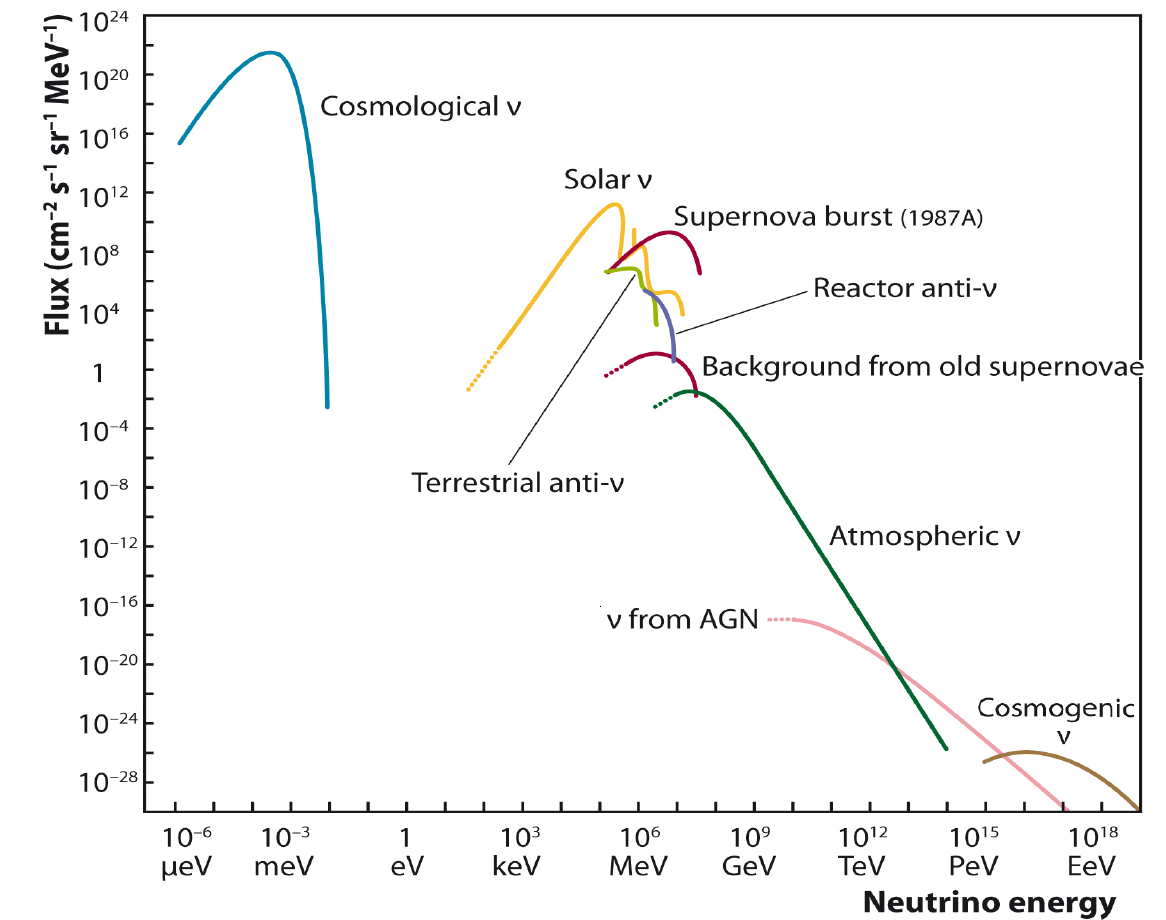
\includegraphics[width=0.7\textwidth]{chapter3/img/neutrinospectrum.png}
\caption{Plot illustrating several neutrino fluxes which cover a huge range of energy. Illustration from \cite{Katz:2011ke}.}
\end{figure}

Cosmic rays are deflected in inter- and extragalactic magnetic fields and therefore their arrival direction at Earth does not hold much pointing information (Fig. \ref{fig:sourceinfo}, left). Light ranging from radio to gamma rays on the electromagnetic spectrum is of a crucial importance in astrophysics but has it's limitations. Photons can be absorbed by interstellar medium, or are trapped in opaque sources. At higher energies ($\approx 10^{14}$ eV) photons interact and produce electron-positron pair ($\gamma + \gamma \rightarrow e^+ + e^-$). Unless the sources are closeby no photons are capable of reaching Earth (see Fig. \ref{fig:sourceinfo}, right). Neutrinos escape from the sources more easily and are not deflected by magnetic fields making them key messengers in identifying cosmic ray accelerators. In the following we will go over the different types of neutrinos which are detectable on Earth.

\begin{figure}[t]
\label{fig:sourceinfo}
\centering
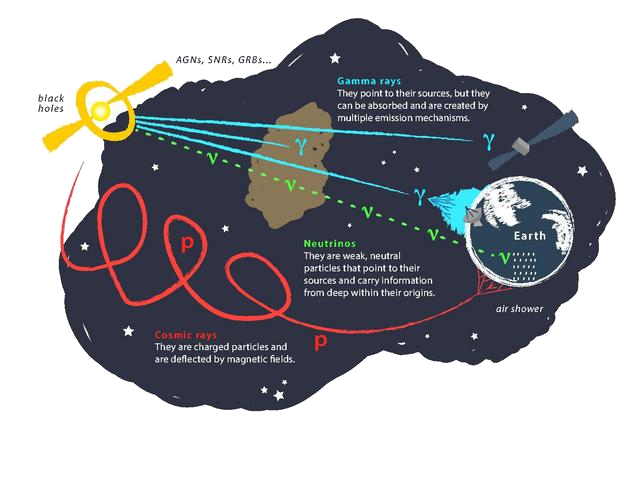
\includegraphics[width=0.4\textwidth]{chapter3/img/sourceinformation_3.jpg}
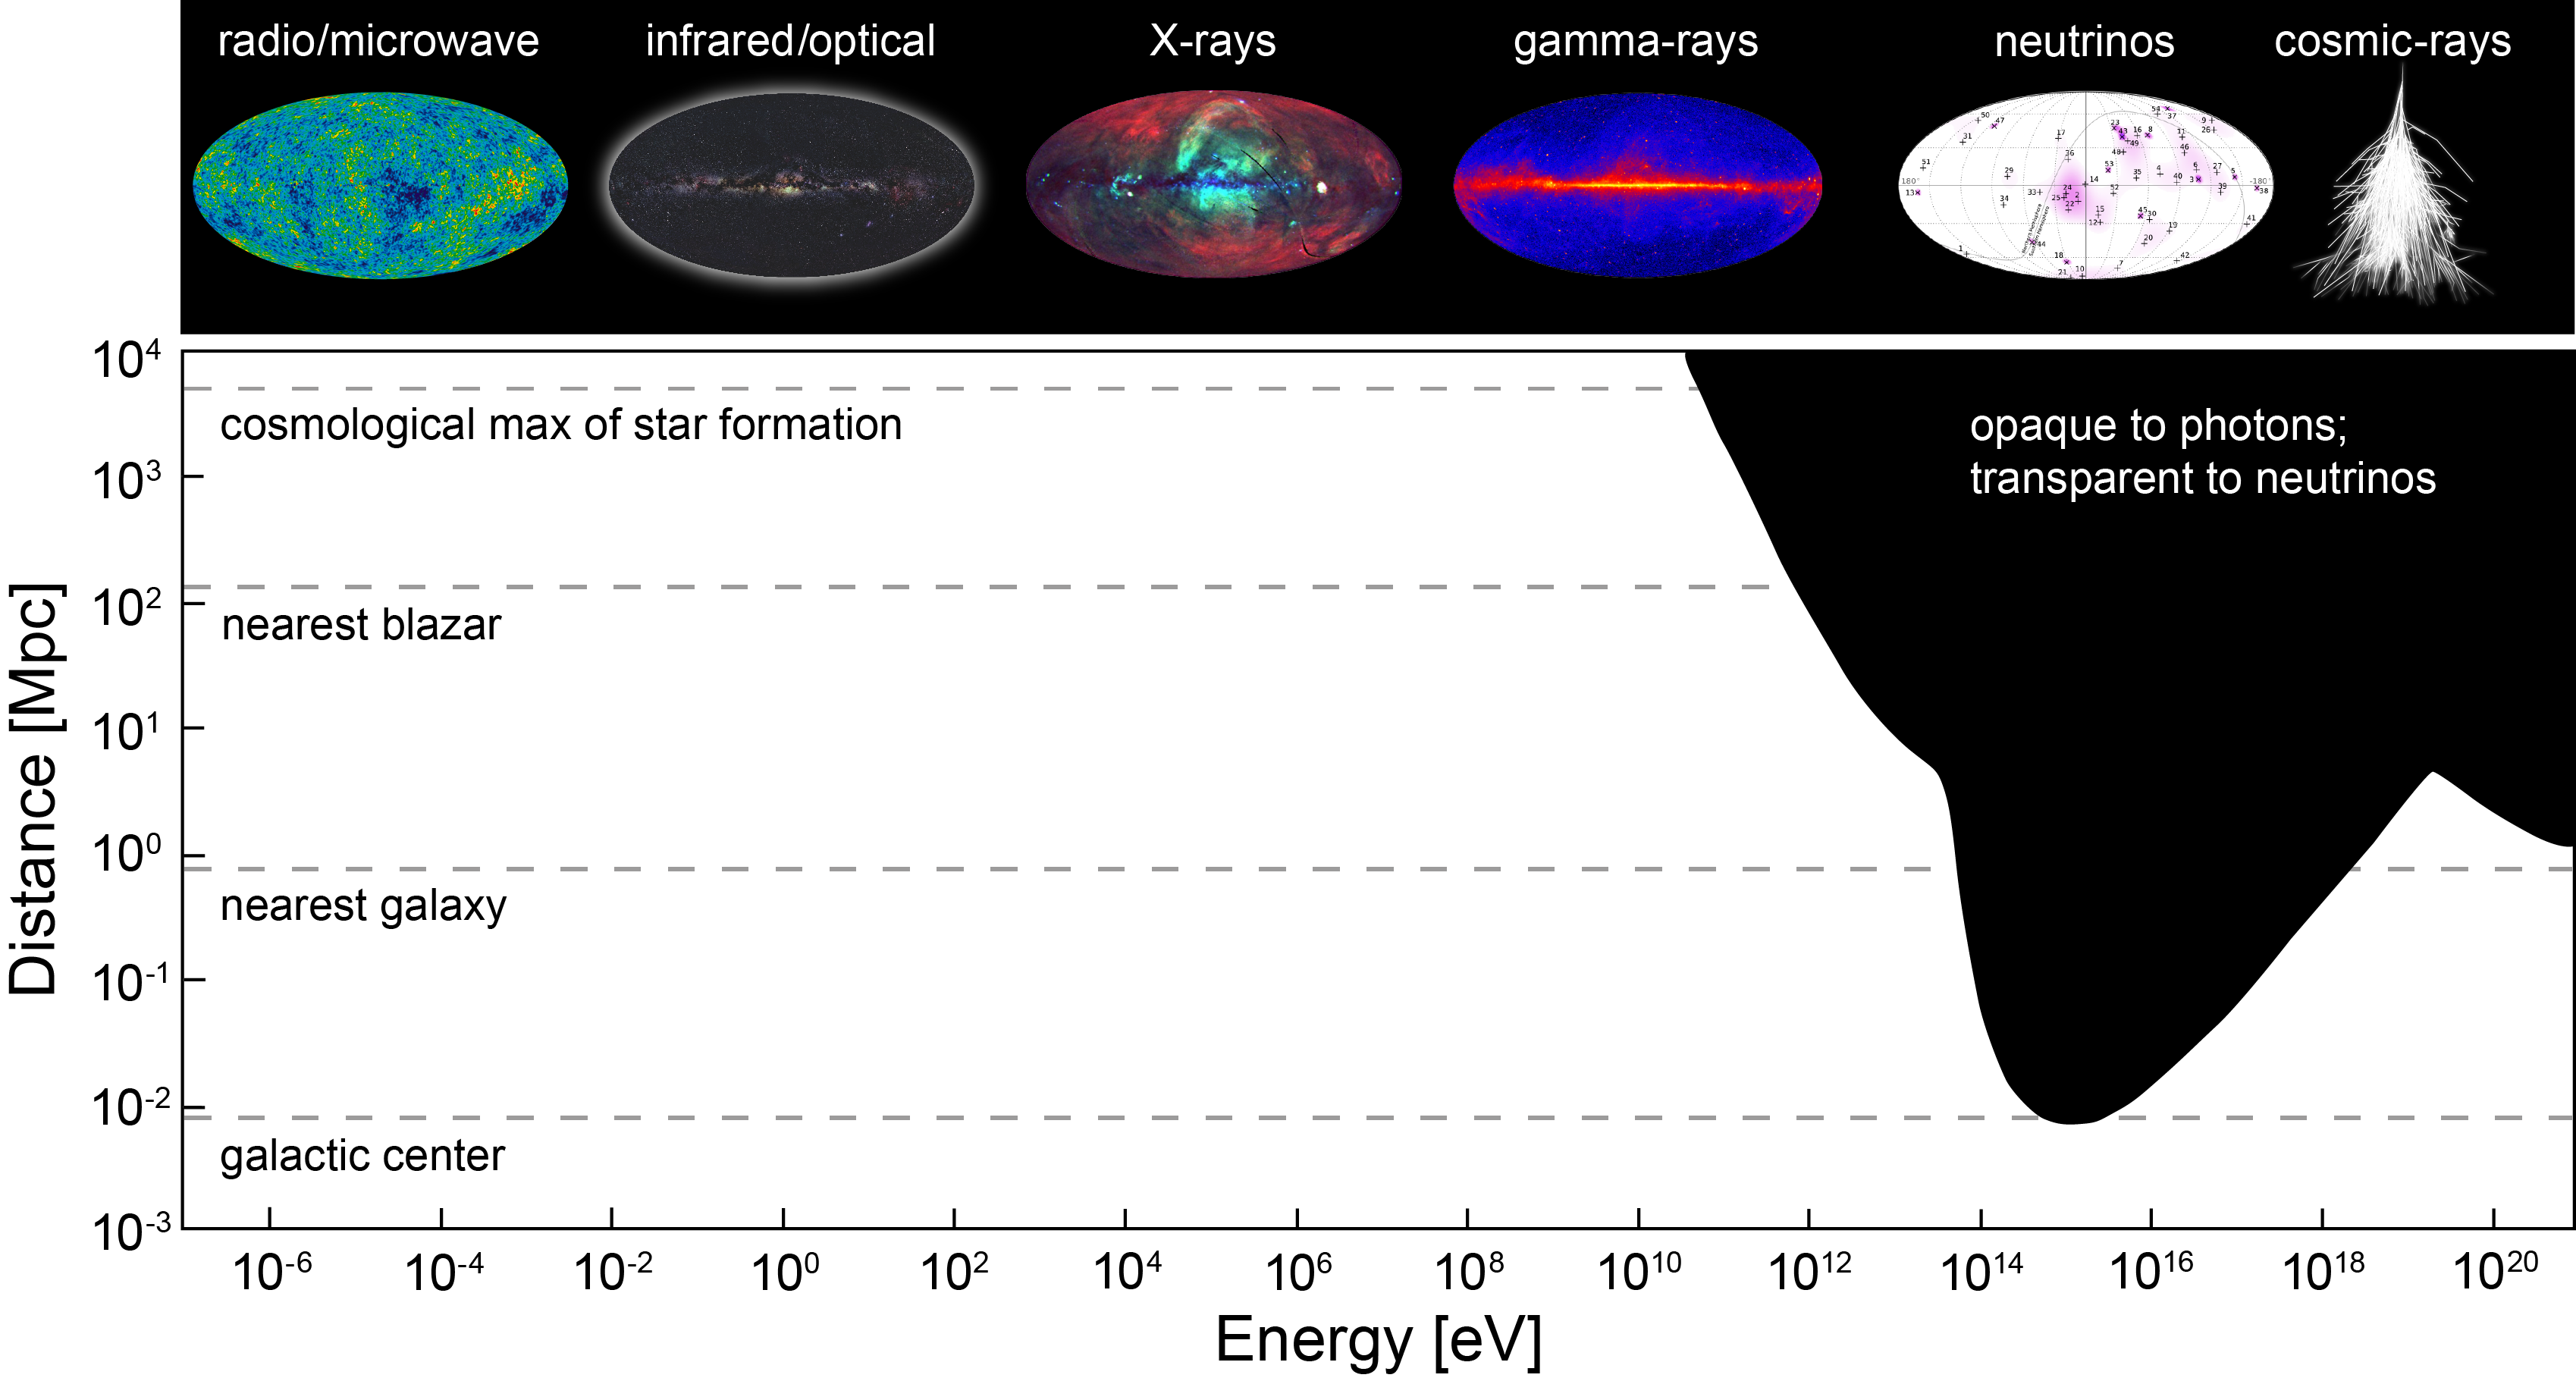
\includegraphics[width=0.59\textwidth]{chapter3/img/opaque-to-photons.png}
\caption{Left: Artist impression of the path that several types of particles travel before reaching Earth. Right: Illustration of the visibility of sources in function of their distance and the photon energy. The signature dip in the photon visibility comes from the pair production peak when photons interact with the CMB. Both illustrations from the IceCube collaboration.}
\end{figure}


\subsection{Conventional}
Neutrinos are produced in large abundances in air showers as explained in \ref{sec:airshowers}. The neutrinos that are produced with low to high energies ($\approx$ MeV to PeV range) are called \textit{atmospheric} or \textit{conventional} neutrinos. They are primarily produced in pion on kaon decay. Due to helicity effects, pion and kaon decay to electron(s) (neutrinos) is strongly suppressed compared to decays into muon(s) (neutrinos). As a result, the ratio of electron neutrinos to muon neutrinos is a factor of around two

\begin{equation}
\frac{N\left( \nu_\mu + \bar{\nu}_\mu\right) }{N\left(\nu_e + \bar{\nu}_e\right)} \approx 2,
\end{equation}
which should be clear when we look at the example of pion decay where the muon decays as well

\begin{align}
\pi^+ &\rightarrow \mu^+ + \nu_\mu \\
& \rightarrow e^+ + \nu_e + \bar{\nu}_\mu + \nu_\mu.
\end{align}
The most referred to calculations for the atmospherical neutrino flux was done by Honda et al. \cite{Honda:2006qj}.
\begin{figure}[t]
\label{fig:neutrinospectrum2}
\centering
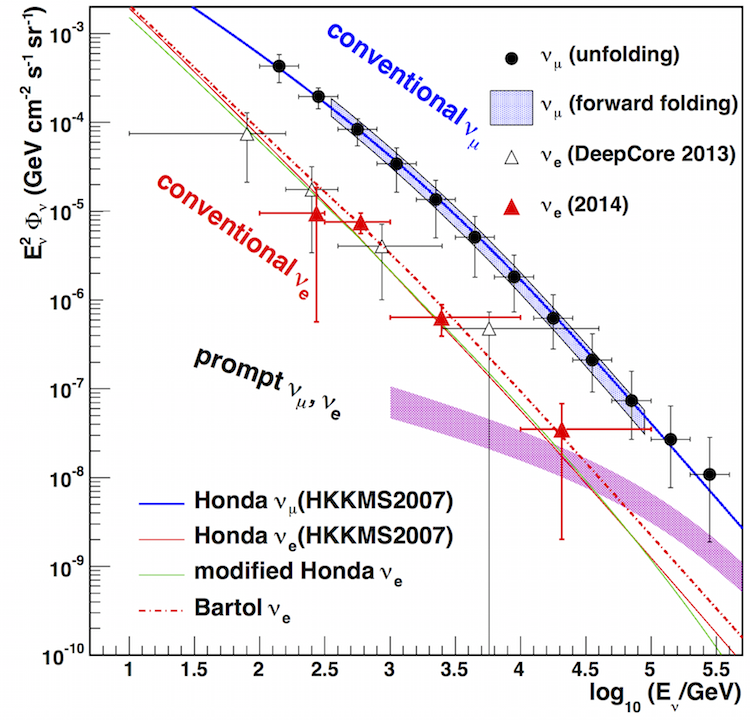
\includegraphics[width=0.39\textwidth]{chapter3/img/neutrinospectrum2.png}
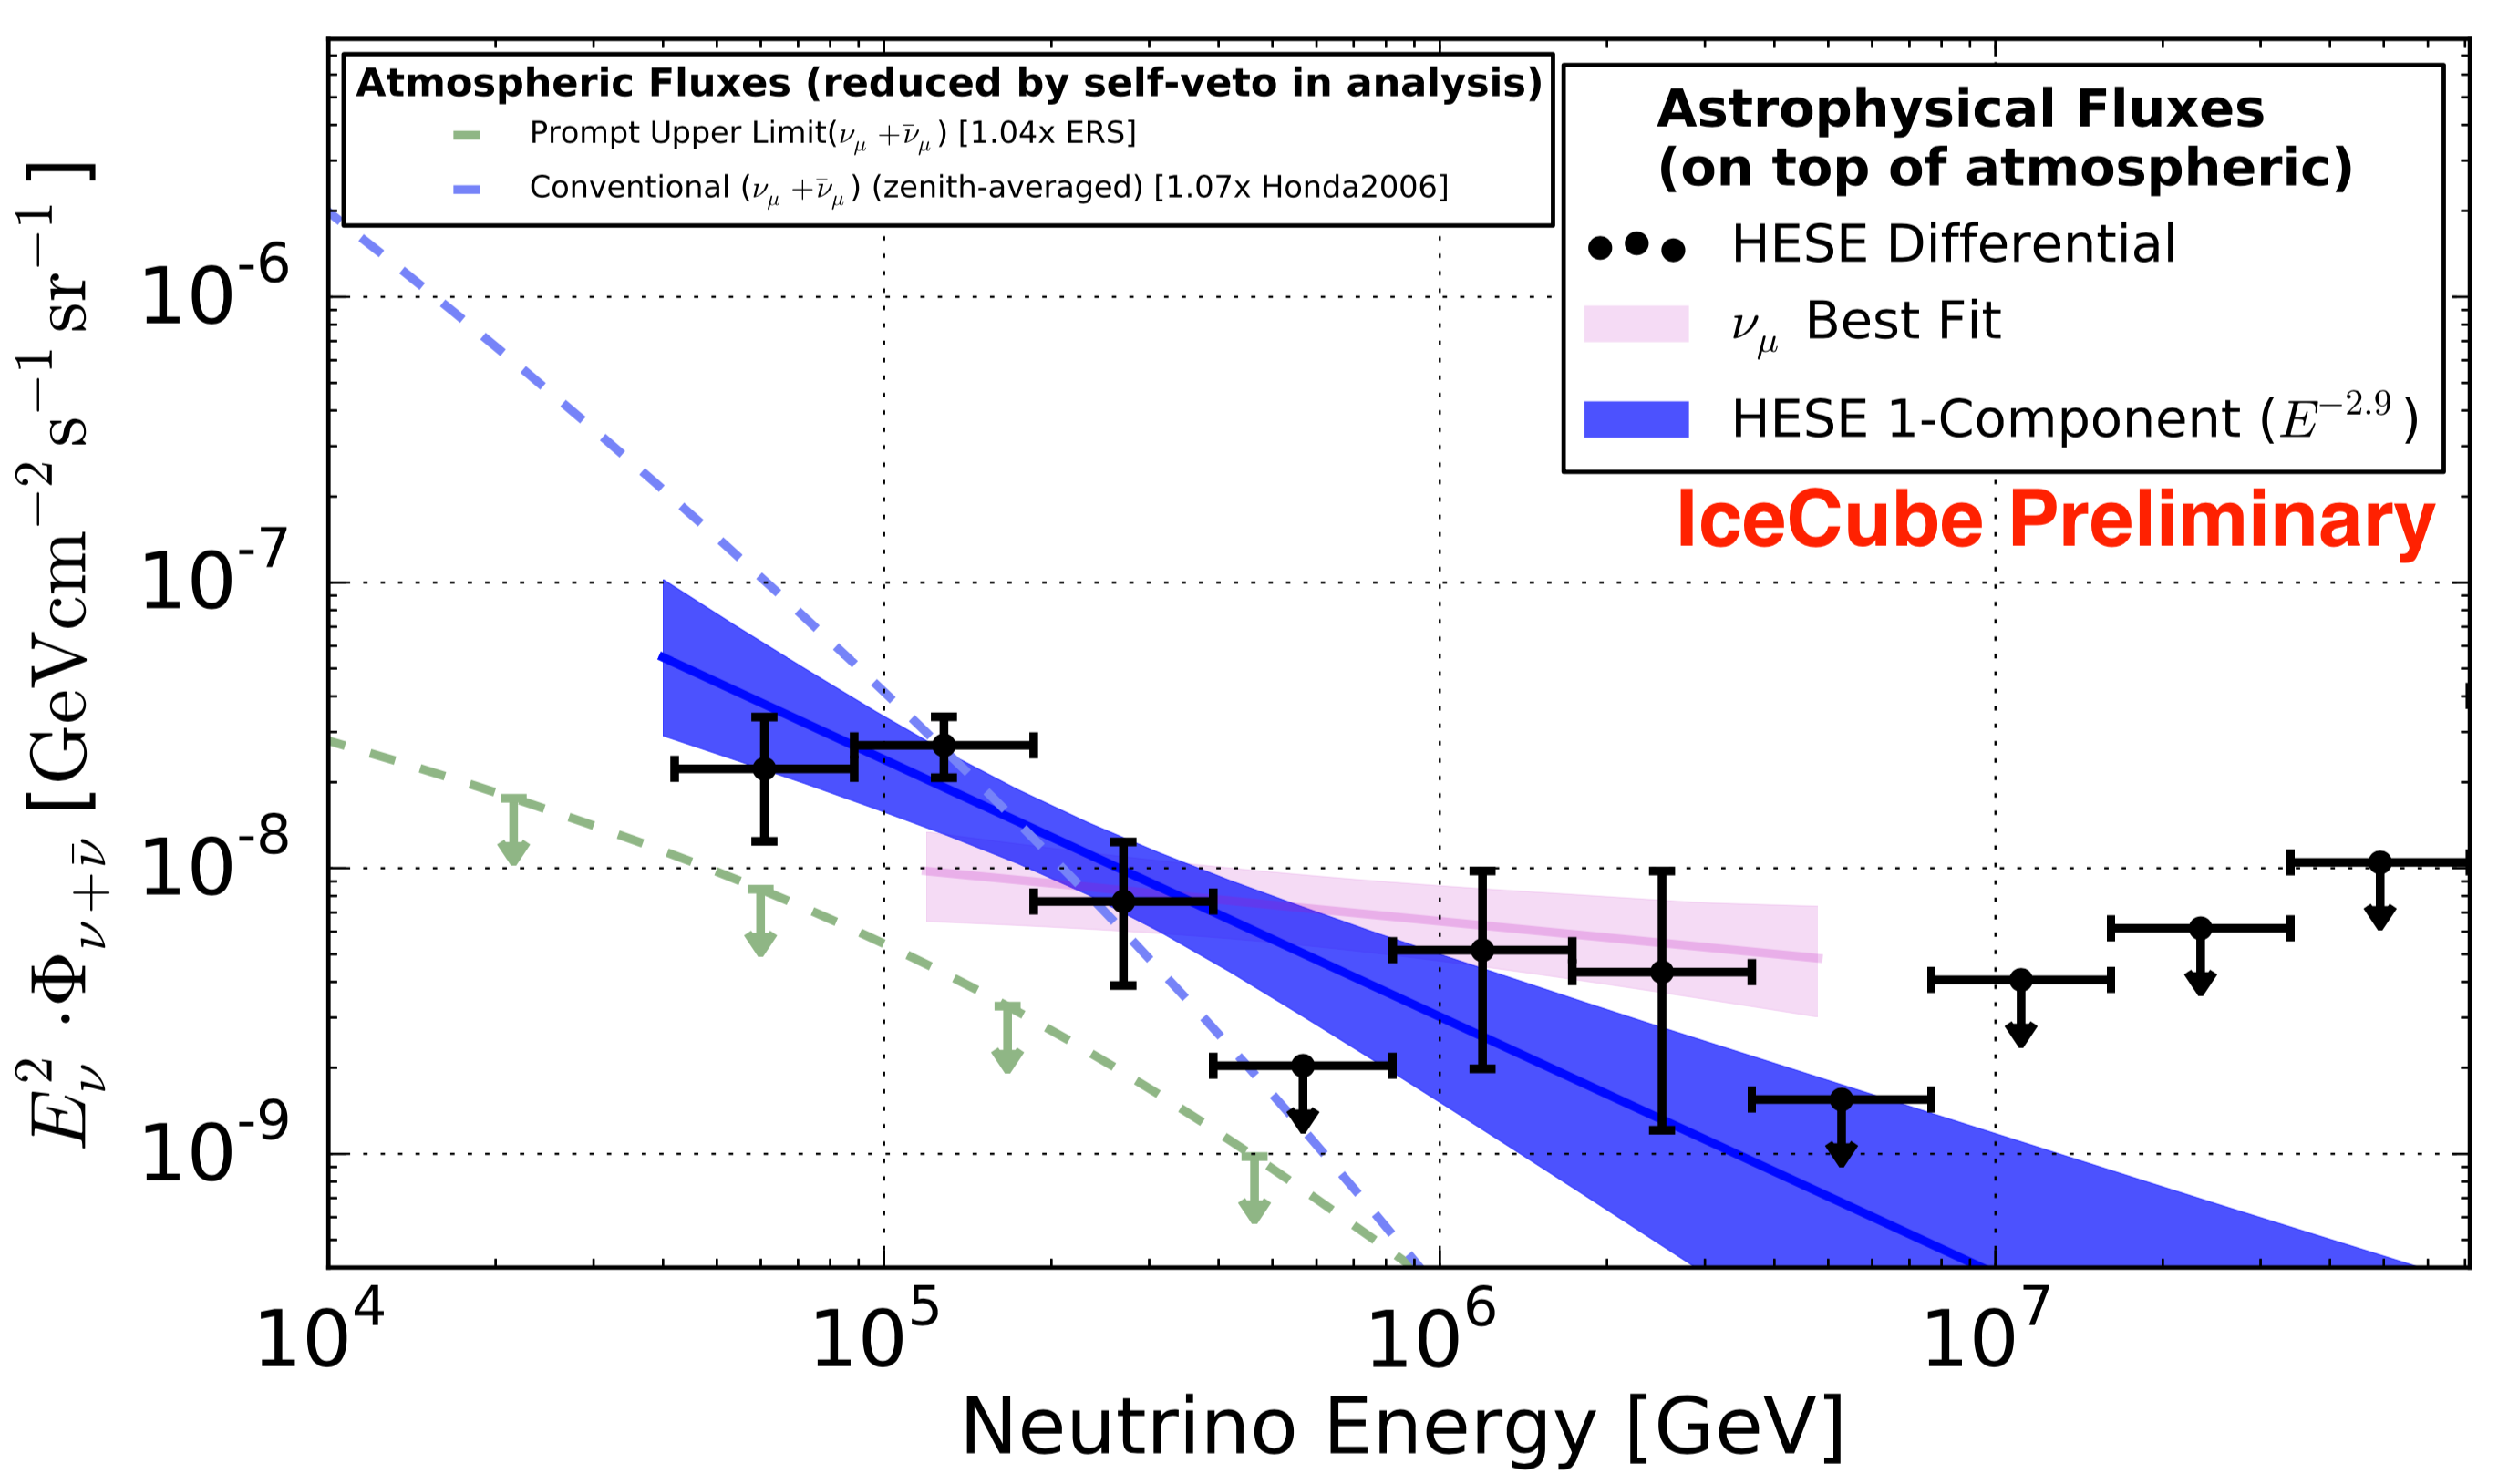
\includegraphics[width=0.6\textwidth]{chapter3/img/astroflux.png}
\caption{Left: Measurement from the IceCube collaboration showing the difference in $\nu_e$ and $\nu_\mu$ flux. Right: Measured differential astrophysical flux using contained events (points) and a fit do that data (blue line and band), compared with the best fit obtained from throug-going $\nu_\mu$ (pink line and band). From Ref. \cite{Aartsen:2017mau}}.
\end{figure}

\subsection{Prompt}
Charmed mesons, also called D mesons, are the lightest particles that contain charm quarks\footnote{$D^0: c\bar{u}, \bar{D}^0: u\bar{c}, D^+: c\bar{d}, D^-: d\bar{c}$}. Hints of charm particles were first seen in cosmic rays in 1971 by Niu et al. \cite{doi:10.1143/PTP.46.1644}. The production of these particles is strongly suppressed, but are expected to exhibit a harder spectrum than conventional neutrinos do. These mesons have short lifetimes (hence the name: prompt) and decay into netrinos independent of their energy and arrival direction. Therefore, their energy spectrum is expected to follow that of primary cosmic rays. Their contribution at higher energies can be non-negligible or even become dominant. To this date is has not been possible to observe this prompt component, but remains an interesting signal in diffuse neutrino searches and could contribute significantly to background expectations.  The most referred to calculations for the prompt neutrino flux was done by Endberg et al. \cite{Enberg:2008te}.
\subsection{Astrophysical}
\label{subsec:astro}
Astrophysical neutrinos are expected to be created when cosmic rays interact close to their interaction sites. Because they are neutral and are unlikely to be absorbed, astrophysical neutrinos are expected to reveal more information about these sources. To first order, these neutrinos would follow the spectrum of cosmic rays at their production. As indicated in section \ref{para:power}, this is equal to an $E^{-2}$ powerlaw spectrum from Fermi shock acceleration. The majority of these neutrinos are expected to arise from decays from pions which were created in these cosmic-ray interactions ($\pi \rightarrow \mu + \nu_\mu$) followed by the muon decay ($\mu \rightarrow e + \nu_e + \nu_\mu$). The resulting flavor ratio fraction is $\nu_e: \nu_\mu: \nu_\tau = 1:2:0$ at the source. Neutrino oscillations across cosmological distances give an expected $\nu_e: \nu_\mu: \nu_\tau = 1:1:1$ expectation at Earth. As can be seen in Fig. \cite{fig:neutrinospectrum2}.

The spectrum is expected to follow the hardest spectrum of the three and therefore dominates at the highest energies.

\subsection{Other neutrino sources}
\subsubsection{Cosmological}
Similar to the photons from the CMB, neutrinos would have been able to decouple from matter only seconds after the Big Bang. Due to the expansion of the universe, the temperature of the neutrinos has dropped to $\approx 1.95K$ due to redshift. At these energies direct detection is near to impossible. They have no measureable effect in large-scale neutrino detectors.
 
Mooie uitleg van redshift: https://www.forbes.com/sites/startswithabang/2016/09/09/cosmic-neutrinos-detected-confirming-the-big-bangs-last-great-prediction/
\subsubsection{Solar}
Nuclear fusion in the Sun is responsible for the production of electron neutrinos and is the largest contribution of neutrinos which can be detected on Earth. 86\% of neutrinos are produced by the proton-proton reaction

\begin{equation}
p + p \rightarrow d + e^+ + \nu_e.
\end{equation}
The remaining part is produced by reactions which involve more heavy particles. Having energies $<$ 20 MeV these neutrinos have no measurable effect in neutrino telescopes.
\subsubsection{Terrestrial neutrinos}
Radioactive decays from $\ce{^{40}K}$, $\ce{^{232}Th}$ and $\ce{^{238}U}$ account for almost all geoneutrinos. The reactions give rise to neutrinos from beta decay \cite{Wan:2016nhe}

\begin{alignat}{2}
\ce{^{40}_{19}K} + e^- &\rightarrow \ce{^{40}_{18}Ar} + \nu_e \ \ &&+1.505 \textrm{ MeV,}\\
\ce{^{40}_{19}K} &\rightarrow \ce{^{40}_{20}Ca} +e^- + \bar{\nu}_e \ \ &&+1.311 \textrm{ MeV,}\\
\ce{^{232}_{90}Th} &\rightarrow \ce{^{208}_{82}Pb} +6\alpha + 4e^- +4\bar{\nu}_e\ \ &&+42.652 \textrm{ MeV,} \\
\ce{^{235}_{92}U} &\rightarrow \ce{^{207}_{82}Pb} + 7\alpha + 4e^- + 4\bar{\nu}_e \ \ &&+46.402 \textrm{ MeV,}\\
\ce{^{238}_{92}U} &\rightarrow \ce{^{206}_{82}Pb} +8\alpha +6e^- + 6\bar{\nu}e \ \ &&+51.698 \textrm{ MeV.}
\end{alignat}
The maximal energies of these neutrinos are again too low to give a contribution to neutrino telescopes.
\subsubsection{Reactor neutrinos}
Nuclear reactors harnass energy from the splitting (fission) of heavy nuclei into lighter fission products. These neutron-rich daughter particles undergo beta decays ($n \rightarrow p+e^-+\bar{\nu}_e$). Reactor neutrinos are therefore always antineutrinos. The energy spectrum reaches a maximum around 10 MeV, making them again invisible for neutrino telescopes. 

\subsubsection{Supernova neutrinos}
The core collapse of stars where electrons and protons are compressed into neutrons as described in ??? dissipates most of it's energy in the production of neutrinos ($e^- + p^+ \rightarrow n + \nu_e$) \cite{Scholberg:2012id}. Depending on the distance of the source to the detector supernovae are only visible in a collective raise of the dark noise of the apparture \cite{Kopke:2011xb}.
\section{Cosmic ray and neutrino detectors}
\label{sec:detectors}

Heel kort: pg 5 Gaisser boek. Zo IC introduceren.

VERITAS, HESS, MAGIC, HAWC, PA, TA, Super-K, Antares, IceCube

Ook dat plotje waarbij je toont dat neutrinos interessanter zijn in hoge E omdat fotonen onzichtbaar worden!

The IceCube Collaboration instead tested the principle using neutrinos. Neutrinos interact with matter through the weak force — one of the four fundamental forces of nature. The influence of the weak force is limited to minute distances. As a result, interactions between neutrinos and matter are extremely improbable, and a neutrino can easily traverse the entire Earth unimpeded. This poses a challenge for physicists trying to study these elusive particles, because almost every neutrino will simply pass through any detector completely unnoticed.




In neutral-current reactions neutrinos lose energy, but are not absorbed

hier tot pg 50?

%----------------------------------------------------------------------------------------
%	CHAPTER 4
%----------------------------------------------------------------------------------------
\chapterimage{MuonWithPhotons_3.png}
\chapter{Relativistic Particles in Matter}
\label{ch:cherenkov}
\begin{flushright}
\textit{\\Hofstadter's Law: It always takes longer than you expect, even when you take into account Hofstadter's Law\\}
\end{flushright}

\noindent Charged particles that travel faster than the speed of light in that material produce light in a process that is called the \textit{Cherenkov effect}. The production of photons makes it possible to detect particles with a non-zero charge (electrons, muons, SMPs, etc.) in a neutrino detector such as the IceCube experiment. This cubic-sized detector is able to register the light that is produced from charged particles in air showers and charged particles that are created when neutrinos interact with the ice around or inside the detector. In this chapter, an overview is given of the Cherenkov effect and the different other physical processes that are visible in the IceCube detector. These signatures have to be accounted for in the background prediction when looking for particles with an anomalous charge. Finally, the energy loss formulae of charged particles in matter are given.


\section{Cherenkov effect}
\label{sec:cherenkoveffect}
From Einstein's works on special and general relativity, it follows that the speed of light in vacuum, $c$, is a universal constant. The speed of light in matter can be significantly lower than that. If a particle travels through a dielectric medium at a speed that is greater than the phase velocity of light in that medium, electromagnetic radiation is emitted. This radiation is called \textit{Cherenkov radiation} and is named after the first person who was able to detect it experimentally, Pavel Cherenkov. He was awarded the Nobel Prize in 1958 for his findings together with Frank and Tamm for their theoretical work on the subject \cite{nobel1958url}.

The velocity of a propagating wave is given by the three-dimensional wave equation

\begin{equation}
\nabla^2\psi = \frac{1}{v^2} \frac{\partial^2 \psi}{\partial^2 t},
\end{equation}
where $\psi$ is the wave function and $v$ its group velocity. From Maxwell's equations and some vector calculus, it is straightforward to find that the wave equation for electromagnetic radiation becomes

\begin{equation}
\nabla^2E = \mu \epsilon \frac{\partial^2 E}{\partial^2 t},
\end{equation}
where $E$ is the electric field and $\mu$ and $\epsilon$ the permeability and permittivity of the medium, respectively. From these equations it is clear that for light in a dielectric medium

\begin{equation}
v = \frac{1}{\sqrt{\mu \epsilon}} = \frac{1}{\sqrt{\mu_r \epsilon_r}}\frac{1}{\sqrt{\mu_0 \epsilon_0}} = \frac{1}{\sqrt{\mu_r \epsilon_r}} \times c \leq c,
\end{equation}
where $1/\sqrt{\mu_0 \epsilon_0} = c$ and $\mu_r$ and $\epsilon_r$ are the relative (to vacuum) permeability and permittivity, respectively and are $\geq 1$. These terms are also written as the refractive index of the medium, $n = \sqrt{\mu_r \epsilon_r}$ and result in

\begin{equation}
v = c/n.
\end{equation}

\noindent When a charged particle moves inside a dielectric medium, it excites the molecules of the medium to the higher levels and excited states. The molecules emit photons in the form of electromagnetic radiation upon returning back to their ground state. According to the \textit{Huygens principle}, the emitted waves move out spherically at the phase velocity of the medium (which can be less than the speed of light in vacuum). If the motion of the particle is slow, the radiated waves bunch up slightly in the direction of motion, but they do not cross. However, if the particle moves faster than the speed of light, the emitted waves add up constructively, leading to a coherent radiation at an angle $\theta_c$ with respect to the particle direction; Cherenkov radiation. The coherent interference is enough to be visible to the naked eye\footnote{The typical blue light in the cooling water at nuclear reactors is also due to this Cherenkov radiation.}. The signature of the effect is a cone of emission in the direction of particle motion. Figure \ref{fig:cherenkov} shows a schematic view of the Cherenkov radiation, illustrating the typical spherical wavefront and the resulting radiation\footnote{The typical cone shape of this effect can be easily seen when observing ducks. If a duck is traveling in a straight line in the water, individual concentric waves can be distinguished and a cone shaped wave is produced behind them.}.

\begin{figure}[t]
\centering
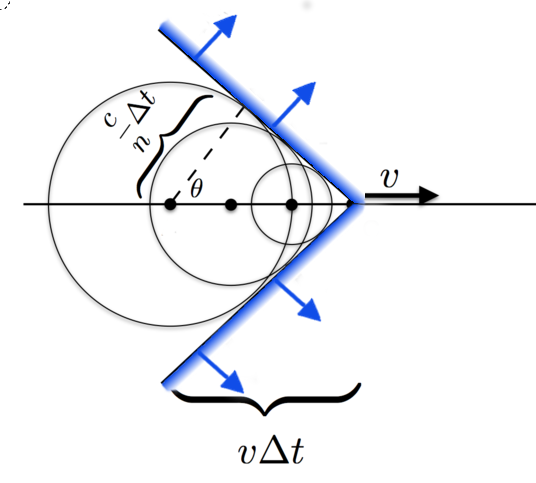
\includegraphics[width=0.6\textwidth]{chapter4/img/cherenkov2.png}
\caption{Schematic view of Cherenkov radiation from a particle traveling at a velocity $v$.}
\label{fig:cherenkov}
\end{figure}

\noindent From the figure we can derive that

\begin{equation}
\cos\theta_c = \frac{\frac{c}{n} \Delta t}{v \Delta t} = \frac{c}{vn} = \frac{1}{\beta n}.
\end{equation} 
Because $-1 \leq \cos\theta_c \leq 1$, the velocity of the charged particle must be $v \geq c/n$. Typical values of $n$ are on the order of 1-2, requiring the particles to be relativistic in order to emit Cherenkov radiation. The number of photons produced per unit path length of a particle with charge $ze$ and per unit energy interval of the photon was calculated by Frank and Tamm, and is often referred to as the Frank-Tamm equation \cite{PDG2018url}

\begin{equation}
\begin{split}
\frac{d^2N}{dE dx} &= \frac{\alpha z^2}{\hbar c} \sin^2 \theta_c = \frac{\alpha^2 z^2}{r_e m_e c^2} \left( 1 - \frac{1}{\beta^2 n^2\left(E\right)} \right)\\
&\approx 370 \sin^2 \theta_c \left(E\right) \textrm{eV}^{-1} \textrm{cm}^{-1} \ \ \ \left( z =1\right),
\end{split}
\end{equation}
where $r_e$ is the classical electron radius, $m_e$ the electron mass and $\alpha$ the fine-structure constant. Equivalently, this equation can be written in function of the wavelength of the photon

\begin{equation}
\label{eq:franktamm}
\frac{d^2N}{dx d\lambda}  = \frac{2\pi \alpha z^2}{\lambda^2} \left(1- \frac{1}{\beta^2 n^2 \left(\lambda \right)} \right),
\end{equation}
where it is clear that the charge of the particle will influence the total Cherenkov light yield. A charge of 1/3$e$ will reduce the light output with a factor of 9 compared to a particle with a charge equal to the electron charge, $e$, such as a muon.\\

\noindent Examples of experiments that make use of this Cherenkov effect are air Cherenkov telescopes such as MAGIC, H.E.S.S and VERITAS that look for the direct and indirect Cherenkov light from gamma rays and cosmic rays. Because the refractive index of air is close to 1 (1.000293 at sea level and smaller with increasing height) the opening angle of the Cherenkov cone is small ($\approx 1^{\circ}$). The particles need to be very relativistic in order for Cherenkov radiation to occur\footnote{Let us assume the refractive index of air at sea level, then, from $E^2/m^2 = \gamma^2 = 1/(1-\beta^2)$, it follows that the minimal energy is $\approx 41$ times its rest mass. Since the refractive index decreases in function of height, the energies of particles interacting with the atmosphere must be even higher.}.

In water and ice, the refractive index is $\approx 1.33$, making $\beta_{min} = 0.75$ and $E_{min} = 1.51 \cdot m_0$. Experiments using water or ice as the interaction medium are Super-Kamiokande, ANTARES and the IceCube experiment.\\

\noindent Most of the light that is emitted from charged particles traveling through matter originates from this Cherenkov effect, provided that their energy is not too high. At higher energies, the amount of secondary particles with an energy high enough to produce Cherenkov effects themselves, becomes so large that this becomes the primary source of light (see Section \ref{sec:energyloss}). This analysis focusses on SMPs that lie below this threshold and we see from Eq. \ref{eq:franktamm} that the charge of the SMP enters in the photon production quadratically. SMPs with a lower charge are therefore expected to produce less photons than minimum ionizing muons.

\section{Neutrino interactions}
\label{sec:neutrinointeractions}
The IceCube experiment is a neutrino detector, but neutrinos have no electromagnetic charge. Neutrinos are only visible through their production of secondary particles with an electromagnetic charge and they emit Cherenkov radiation in the ice. Here, we briefly describe how these interactions take place.\\

\noindent Neutrinos interact with matter through both charged current (CC) and neutral current (NC) processes. In the former, the mediator particle is a charged $W$ boson resulting in a charged lepton in the final state. In the latter, the mediator particle is the neutral $Z$ boson. Both interaction types have a resulting hadronic component as daughter particles. The interactions can be written as

\begin{alignat}{2}
\nu_l \left(\bar{\nu}_l\right) + N &\xrightarrow{W} l^- \left(l^+\right) + X^{+\left(-\right)} \ \ && \left(CC\right)\\
\nu_l \left(\bar{\nu}_l\right) + N &\xrightarrow{Z} \nu'_l \left(\bar{\nu}'_l\right) + X && \left(NC\right),
\end{alignat}
where $l$ is the lepton flavor ($e,\mu,\tau$), $N$ denotes the initial hadronic state of the nucleus and $X$ the final hadronic state. These interactions are illustrated in Figure \ref{fig:feynmanneutrino}.\\
\newline
The charged leptons and hadrons lead to light production via gamma ray production and Cherenkov radiation. With the right material, it is possible to detect this light production and reconstruct some of the neutrino's characteristics. \textcolor{red}{Because the light production depends on the square of the charge of a particle, the IceCube detector is not powerful in detecting if the primary particle was a neutrino or antineutrino\footnote{Although it is not possible to distinguish neutrino from antineutrino events on an event-by-event basis, there are ways to look at differences. One example is to look at inelasticity effects as done in Ref. \cite{Aartsen:2018vez}.}.}

\begin{figure}[t]
\centering
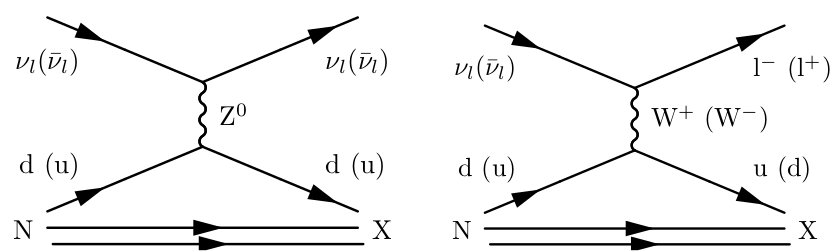
\includegraphics[width = 0.9\textwidth]{chapter4/img/feynmanneutrino.png}
\caption{Feynman diagrams of NC (\textit{left}) and CC (\textit{right}) neutrino interactions. $l$ is the lepton flavor ($e,\mu,\tau$), $N$ denotes the initial hadronic state of the nucleus and $X$ the final hadronic state. The antineutrino interactions are given in brackets.}
\label{fig:feynmanneutrino}
\end{figure}


\section{Propagation}
\label{sec:propagation}
As described in Section \ref{sec:neutrinointeractions}, neutrinos give rise to several types of interactions in the surrounding medium. There are three characteristic signatures, which are the main interest in the IceCube detector (illustrated in Figure \ref{fig:ICinteractions}).

\begin{figure}[t]
\centering
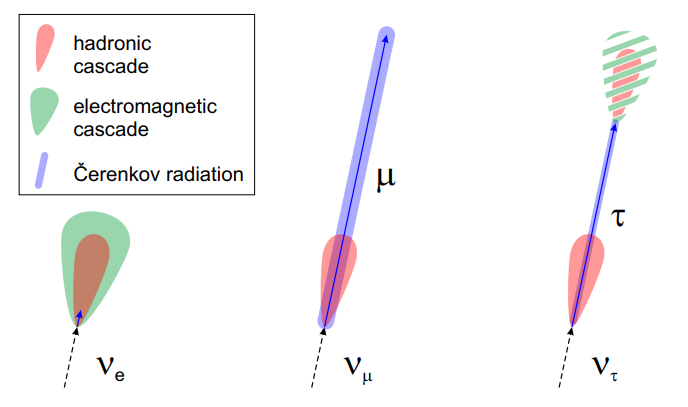
\includegraphics[width=0.7\textwidth]{chapter4/img/ICinteractions.png}
\caption{Schematic view of the charged current neutrino signatures in matter. At each interaction point there is a hadronic cascade (red). Every hadronic cascade has electromagnetic sub-showers which are not illustrated here. Muons and energetic taus can give rise to tracks. The electromagnetic and hadronic cascades have a more spherical shape but are exaggerated for illustrative purposes in the figure. Illustrations from Ref. \cite{Wallraff}.}
\label{fig:ICinteractions}
\end{figure}

\subsection{Cascades}
\subsubsection{Electrons and photons}

In a charged current electron-neutrino interaction, the energetic electron gives rise to a shower of gamma rays (bremsstrahlung) and positrons and electrons (pair production). Positrons and electrons in their turn emit new gamma rays and this process continues until the photon energies fall below the pair production threshold. Because electrons/positrons lose their energy fast, they are almost immediately stopped, giving an \textit{electromagnetic cascade} an almost spherical shape.

Let us assume $E_0$ is the energy of the incoming electron. In a very simplistic toy model one can say that an electron emits one photon after one radiation length, $X_0$. A photon will decay into an electron-positron pair after approximately one radiation length too\footnote{In fact, one radiation length actually implies $1/e$ times the initial energy. Assuming the electron loses half its energy to the photon, and with 0.63/0.5 $\approx 1$, the radiation length is indeed almost equal to the average length an electron travels before emitting a photon. The total probability for pair production per unit radiation length from a photon is $\approx 7/9$, where we again assume that this is $\approx 1$.}. At every decay or radiation process, it is assumed that the daughter particles carry 1/2 of the energy. After $t$ steps, the energy is equal to

\begin{equation}
E(t) = \frac{E_0}{2^t}.
\end{equation}
The number of particles will be equal to

\begin{equation}
N(t) = 2^t.
\end{equation}
At a critical energy $E_c$, the multiplication process stops (as pair production dominates over bremsstrahlung) and we find

\begin{equation}
t_{max} = \frac{\ln\left(\frac{E_0}{E_c}\right)}{\ln 2},
\end{equation}
the total longitudinal length of an electromagnetic shower is thus approximately equal to

\begin{equation}
X = X_0 \frac{\ln\left(\frac{E_0}{E_c}\right)}{\ln 2}.
\end{equation}
This logarithmic dependence on the energy of the initial particle will therefore result into elongations of a couple of meters at most. Typical values in ice are $X_0 \approx 40$ cm and $E_c \approx 80$ MeV.

\subsubsection{Hadrons}
In the case of neutral current events, the breakup of the struck nucleus leads to charged byproducts. These byproducts can re-interact in the medium and produce neutral pions that decay into gamma rays. These particles again die out quickly, resulting in a spherical emission of light for \textit{hadronic cascades}. The basic development of hadronic cascades in space is very similar to that of electromagnetic ones, but with important differences in energy loss, particle content, lateral spread and fluctuations. Hadronic cascades contain particles heavier than electrons, that have a higher Cherenkov threshold. A fraction of them are slow neutrons, which do not produce any light. Neutral pions produce gamma rays. Charged pions, on the other hand, can decay into muons and muon neutrinos; long-ranged particles that do not contribute to the cascading process. Finally, a non-negligible fraction of the energy is lost in the hadronic binding processes.

The light yield will be smaller than the one obtained from an electromagnetic cascade of equal initial energy and with much larger event-by-event variations. 


\subsection{Muon tracks}
Muons are produced in charged current muon-neutrino interactions and travel much further than electrons and positrons. The relativistic muon will produce light according to the Frank-Tamm equation, Eq. \ref{eq:franktamm}, resulting in \textit{direct Cherenkov radiation}. Ionization, bremsstrahlung, pair production, and photonuclear interactions (see Section \ref{sec:energyloss}) are also capable of producing relativistic secondary particles that produce \textit{indirect Cherenkov radiation}. Both effects result in a Cherenkov cone with a diffuse light emission from the track in all directions behind it. 

\subsubsection{Energy loss}
\label{subsub:energyloss}
Below 1 TeV, muons will lose most of their energy to ionization losses. A charged particle traversing matter ionizes the material around it. When the energy transfer is high enough, electrons can be stripped away from their atoms, resulting in \textit{delta electrons}. As can be seen in Figure \ref{fig:energyloss}, ionization losses have only a very weak energy dependence. It is therefore very difficult to distinguish for example a 50 GeV from a 500 GeV muon as the direct Cherenkov light production will be similar (Eq. \ref{eq:franktamm}) and the energy loss is from the almost-energy-independent ionization.

Above 1 TeV, however, the muon, on average, loses more energy to stochastic\footnote{In this context we mean that the energy losses are not deterministic: it is impossible to know when an interaction of this kind will occur. One can only make estimations of their \textit{expected} effects.} effects. Here, effects such as bremsstrahlung, pair production and the photonuclear effect dominate over ionization (see Section \ref{sec:energyloss}). Therefore, indirect Cherenkov production starts to dominate and makes the energy estimation much easier.\\

\begin{figure}[t]
\centering
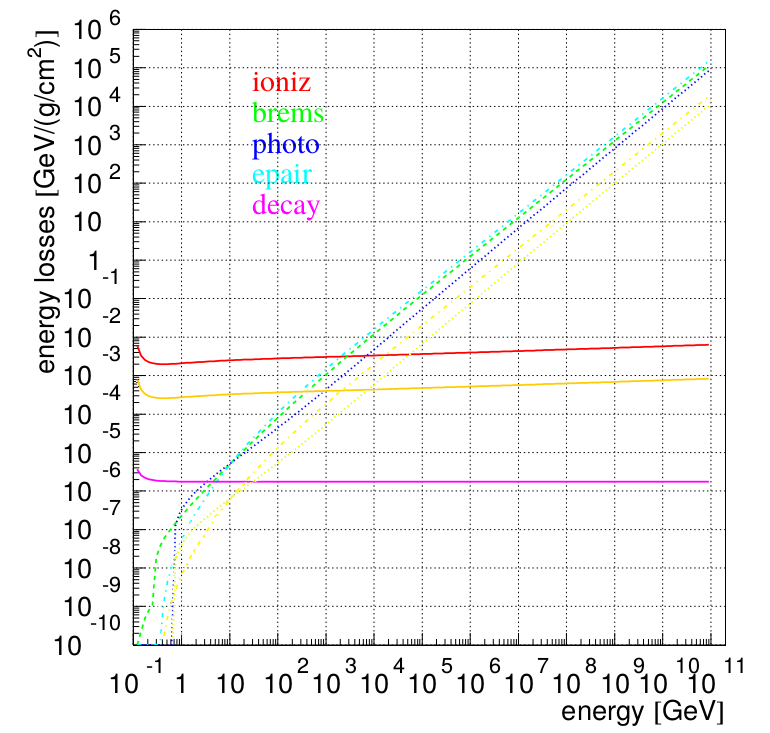
\includegraphics[width = 0.7\textwidth]{chapter4/img/muonenergyloss_extra.png}
\caption{Muon energy loss from ionization (upper solid curve, red), bremsstrahlung (dashed, green), photonuclear (dotted, blue), pair production (dashed-dotted, cyan) and decay (lower solid curve, purple). Additionally, the expected energy losses of a muon with charge 1/3 are shown in orange/yellow. Ionization, photonuclear and pair production scale with $z^2$, giving a factor 9 difference. Bremsstrahlung, which has a $z^4$ dependence is left out.}
\label{fig:energyloss}
\end{figure}

\noindent The average energy loss from ionization and stochastic effects along the muon trajectory can be parameterized by \cite{Barrett:1952woo} 

\begin{equation}
\label{eq:energyloss}
- \frac{dE}{dx} = a + b \cdot E_\mu,
\end{equation}
where $a$ and $b$ are obtained by fitting and can be found in Table \ref{tab:energylossconstants}. Here $a$ corresponds to the ionization energy loss (given by Eq. \ref{eq:ioniz}), and $b$ corresponds to the sum of $e^+e^-$ pair production, bremsstrahlung, and photonuclear contributions. The muon range can be found by integrating Eq. \ref{eq:energyloss}

\begin{equation}
\begin{split}
R_\mu \approx \frac{1}{b} \ln \left( \frac{E_\mu}{E_{th}} +1 \right),
\end{split}
\end{equation}
with $E_{th} = a/b = 720$ GeV, the energy threshold above which stochastic effects are dominant.\\


% Please add the following required packages to your document preamble:
% \usepackage[table,xcdraw]{xcolor}
% If you use beamer only pass "xcolor=table" option, i.e. \documentclass[xcolor=table]{beamer}
\begin{table}[]
\caption{Best fits for muon energy loss parameters $a$ and $b$ from Eq. \ref{eq:energyloss}. Fits from Ref. \cite{Chirkin:2004hz}.}
\label{tab:energylossconstants}
\begin{center}
\begin{tabular}{|l |c|c|}
\hline
{\cellcolor[HTML]{F1A91E} \textbf{Medium}}   & \cellcolor[HTML]{F1A91E}{$a \left(\frac{\textrm{GeV}}{\textrm{mwe}^\dagger}\right)$} & \cellcolor[HTML]{F1A91E}{$b \left(\frac{10^{-3}}{\textrm{mwe}}\right)$} \\ \hline 
\textbf{Air}    & 0.281                                                                                             & 0.347                                                                                        \\ \hline
\textbf{Ice}      & 0.259                                                                                             & 0.363                                                                                        \\ \hline
\textbf{Fr. Rock} & 0.231                                                                                             & 0.436                                                                                        \\ \hline
\textbf{St. Rock} & 0.223                                                                                             & 0.463                                                                                        \\ \hline
\end{tabular}
\end{center}
\centering  ${}^\dagger${\small Mwe stands for ``meter water equivalent'', a unit often used in cosmic ray physics. A detector shielded by matter equal to 100 mwe would be equally shielded from cosmic rays if it were 100 meters below water.}
\end{table}

\noindent SMPs will have very similar signatures in the IceCube detector as we have assumed that they behave leptonically (Section \ref{sec:properties}). The tracks will be dim compared to muon tracks due to the charge dependence in the Cherenkov effect (Section \ref{sec:cherenkoveffect}).

\section{Energy loss formulae}
\label{sec:energyloss}
As mentioned in Section \ref{subsub:energyloss}, secondary interactions such as bremsstrahlung, pair production and photonuclear effect, become non-negligible at certain energies. At high energies (> 1 TeV for muons) the Cherenkov light of the secondary particles will have a significant contribution additional to the Cherenkov light coming from the primary particle. These effects are taken into account in IceCube simulations and are of great importance for high-energy muons. Since these interactions are electromagnetic in nature, they will also play a role for SMP particles, yet these effects are small for the SMPs with a primary focus on lower energies.

In this section we go over the four main components of secondary interactions. This section is largely based on the findings in Ref. \cite{Chirkin:2004hz}. The energy of the secondary particles will be expressed by $\nu = v E$, with $E$ the energy of the incident particle and $v$ the fraction of the energy transfer. Secondary interactions occur at all energy levels and become approximately continuous in nature below a certain energy threshold. Therefore, in many codes $v_{cut}$ is implemented as a lower bound equal to 0.05 and a $\nu_{cut}$ equal to 500 MeV \cite{dimaspice}. 

\subsection{Ionization}
Fast charged particles that move through matter interact with the electrons of atoms in the material. The interaction excites or ionizes the atoms. The Feynman diagram of this interaction is given in Figure \ref{fig:feynmanionizbrems} (left). 

The cross section is expressed as 

\begin{equation}
\begin{split}
\frac{d^2N}{d\nu dx} = &\frac{1}{2} K z^2 \frac{Z}{A} \frac{1}{\beta^2} \frac{1}{
\nu^2} \left[1-\beta^2 \frac{\nu}{\nu_{max}} + \frac{1}{2} \left(\frac{\nu}{E(1+1/\gamma)} \right)^2 \right],\\
&\textrm{with   } \nu_{max} = \frac{2 m_e (\gamma^2 -1)}{1+2\gamma \frac{m_e}{m_t} +\left(\frac{m_e}{m_t}\right)^2}
\end{split}
\end{equation}
where negligible terms are left out and $K$ is equal to $4\pi N_A r_e^2 m_e c^2$, $N_A$ is Avogadro's number, $r_e$ the classical electron radius, $m_e$ the electron mass, $z$ the charge of the particle (in units of the electron charge), $Z$ the atomic number of the absorber, $A$ the atomic mass of the absorber and $m_t$ the mass of the throughgoing particle.

This interaction leads to an energy loss of the traveling particle and is expressed by the Bethe-Bloch formula \cite{PDG2018url}

\begin{equation}
\label{eq:ioniz}
\begin{split}
-\left\langle\frac{dE}{dx}\right\rangle = K z^2 \frac{Z}{A \beta^2} &\left[\frac{1}{2} \ln \left(\frac{2 m_e \beta^2 \gamma^2 \nu_{upper}}{I\left(Z\right)^2} \right) -\frac{\beta^2}{2}  \left(1+\frac{\nu_{upper}}{\nu_{max}} \right) + \frac{1}{2} \left( \frac{\nu_{upper}}{2E(1+1/\gamma)}\right)^2 - \frac{\delta}{2}\right], \\ 
&\textrm{where } \nu_{upper} = \min(\nu_{cut},\nu_{max}) 
\end{split}
\end{equation} 
where $I$ is the mean excitation energy of the absorber. The density correction $\delta$ can be found in the corresponding literature \cite{Chirkin:2004hz}.

For particles in the region of $0.1 \leq \beta \gamma \leq 1000$ this is the dominant factor in the mean energy loss. 

\begin{figure}
\centering
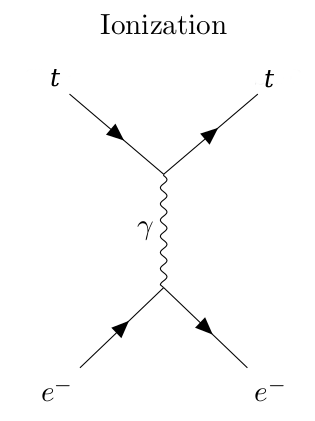
\includegraphics[width = 0.35\textwidth]{chapter4/img/Feynman_Ionization_2.png}
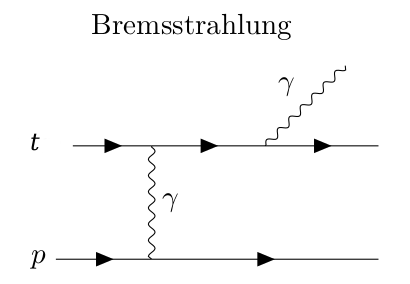
\includegraphics[width = 0.48\textwidth]{chapter4/img/Feynman_Bremsstrahlung_2.png}
\caption{Feynman diagrams of an ionization interaction (\textit{left}) and bremsstrahlung (\textit{right}). \textit{t} denotes the primary particle.}
\label{fig:feynmanionizbrems}
\end{figure}


\subsection{Bremsstrahlung}
Charged particles that decelerate by another charged particle lose kinetic energy that is converted into radiation. This phenomena is known as \textit{bremsstrahlung} and is illustrated in Figure \ref{fig:feynmanionizbrems} (right). The cross section may be represented by the sum of an elastic component and two inelastic components,

\begin{equation}
\sigma = \sigma_{el} + \Delta \sigma^{in}_a + \Delta \sigma^{in}_n,
\end{equation}
where $\sigma_{el}$ denotes the cross section for the Coulomb scattering of the particle off the atomic nucleus and the two other terms are corrections that account for additional processes, in which the bremsstrahlung is accompanied by a change of electronic or nuclear structure of the atom in the final state.

\subsubsection{Elastic component}
\begin{equation}
\begin{split}
\sigma_{el} (E,v) = \frac{ \alpha}{v} \left(2 z^2 Z \frac{m_e}{m_t} r_e\right)^2
 &\left(\frac{4}{3} - \frac{4}{3}v +v^2 \right) \left[\ln \left[\frac{m_t}{\delta}\right] - \frac{1}{2} - \Delta \sigma^{el}_a -\Delta \sigma^{el}_ n \right],\\
& \textrm{ \ \ where \ \ } \delta \approx \frac{\mu^2 \omega}{2E(E-\omega)},
\end{split}
\end{equation}
where $\alpha$ is the fine structure constant and $\omega$ the photon's frequency with $\hbar = 1$. The atomic and nuclear form factors are equal to

\begin{equation}
\label{eq:formfactors}
\begin{split}
&\Delta \sigma^{el}_a(\delta) = \left[ 1+ \frac{1}{\delta \sqrt{e} BZ^{-1/3}/m_e}\right] \\
&\Delta \sigma^{el}_n(\delta) = \left[\frac{D_n}{1+\delta (D_n \sqrt{e} -1)/m_t}\right].
\end{split}
\end{equation}
Values for $B$ and $D_n$ can be found in Ref. \cite{Kelner:1995hu}, here, $e$ is the base of the natural logarithm ($\approx 2.718$) and other constants are as defined in Eq. \ref{eq:ioniz}. Other parameterizations can be found in the corresponding literature \cite{Chirkin:2004hz}. 
%mu hier dimensieloos (zie inleiding)

\subsubsection{Inelastic component}

The effect of nuclear excitation can be evaluated as

\begin{equation}
\Delta \sigma^{in}_n = \frac{1}{Z} \Delta \sigma^{el}_n; (Z \neq 1),
 \end{equation}
where $\Delta \sigma^{el}_n$ is defined in Eq. \ref{eq:formfactors}.

In the case of atomic excitation, one accounts for bremsstrahlung whereby photons radiate from the primary particle and where photons radiate from the electrons of the atom. This factor is equal to

\begin{equation}
\Delta \sigma^{in}_a \approx \frac{1}{Z} \ln \left[ \frac{m_t/\delta}{\delta m_t/m_e^2 + \sqrt{e}} \right] - \ln\left[1+ \frac{m_e}{\delta \sqrt{e} B' Z^{-2/3}} \right],
\end{equation}
where $B'=1429$ for $Z > 2$, $B' = 446$ for $Z=1$ and $e$ is again the base of the natural logarithm.
\subsection{Photonuclear}
The photonuclear interaction of leptons is the process by which a lepton scatters inelastically with a nucleon or nucleus. Through a virtual photon exchange, hadrons are produced, as is illustrated in Figure \ref{fig:feynmannuclpairprod} (left). The cross section formula is given by

\begin{equation} 
\begin{split} 
\frac{d\sigma}{dv} &= \frac{z^2 \alpha}{2\pi} A \sigma_{\gamma N} v  \Bigg \lbrace  0.75 G(x) \Bigg [\kappa \ln \left(1+\frac{m_1^2}{t}\right) \\
& -\frac{\kappa m_1^2}{m_1^2 + t} - \frac{2 m_t^2}{t} + \frac{4 m_t^2}{m_1^2} \ln \left(1+ \frac{m_1^2}{t} \right)  \Bigg] \\
& + 0.25 \left[ \left(\kappa + \frac{2m_t^2}{m_2^2} \right) \ln \left(1+\frac{m_2^2}{t} \right) - \frac{2m_t^2}{t}\right]\\
& + \frac{m_t^2}{2t} \left[ 0.75 G(x) \frac{m_1^2 -4t}{m_1^2 +t} +0.25 \frac{m_2^2}{t} \ln \left(1+\frac{t}{m_2^2} \right) \right] \Bigg \rbrace,\\
& \textrm{where \ \ } t = Q_{max}^2 = \frac{m_t^2 v^2}{1-v}, \ \ \kappa = 1-\frac{2}{v} + \frac{2}{v^2}, \\
& m_1^2 = 0.54 \textrm{ GeV}^2, \ \ \textrm{and \ \ \ } m_2^2 = 1.8 \textrm{\ GeV}^2.
\end{split} 
\end{equation}
Parameters that aren't defined here can be found in the corresponding literature \cite{Chirkin:2004hz}.

%\begin{equation}
%\sigma_{\gamma N}
%\end{equation}
\subsection{Pair production}
\label{subsec:pairprod}
Pair production occurs when the virtual photon radiated from the primary particle or proton splits into an electron-positron pair or muon-antimuon pair, as is illustrated in Figure \ref{fig:feynmannuclpairprod} (right). The differential cross section is equal to
 
\begin{equation}
\begin{split}
&\frac{d\sigma(E,v,\rho)}{dvd\rho} = \frac{2}{3\pi} Z(Z+\zeta)(z \alpha r_e)^2 \frac{1-v}{v} \left(\Phi_e + \frac{m_e^2}{m_\mu^2} \Phi_\mu \right), \\
& \textrm{ where \ \ } v = (\epsilon_+ + \epsilon_-)/E, \ \ \rho = (\epsilon_+ - \epsilon_-)/(\epsilon_+ + \epsilon_-),
\end{split}
\end{equation}
and $\epsilon_+$ and $\epsilon_-$ denote the energies of the positively and negatively charged electrons/muons. The parameters not described in detail can be found in the corresponding literature \cite{Chirkin:2004hz}.

\begin{figure}
\centering
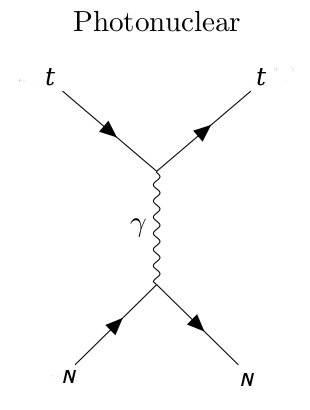
\includegraphics[width = 0.35\textwidth]{chapter4/img/Feynman_PhotoNuclear_2.png}
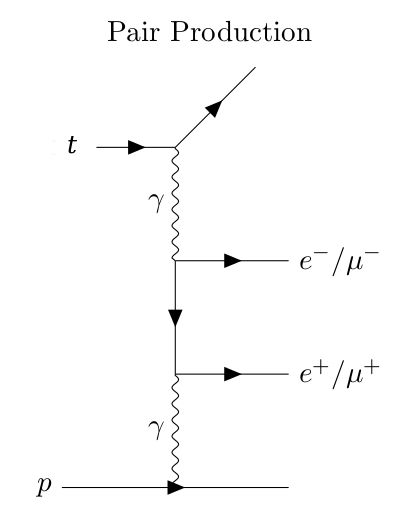
\includegraphics[width = 0.35\textwidth]{chapter4/img/Feynman_PairProduction_2.png}
\caption{Feynman diagrams of a photonuclear interaction (\textit{left}) and pair production (\textit{right}). $t$ denotes the primary particle.}
\label{fig:feynmannuclpairprod}
\end{figure}

\subsection{Conclusion}
\label{sub:energylossconclusion}
From the previous discussion we can conclude that the charge enters in the energy loss formulae quadratically for ionization, pair production and the photonuclear effect. Bremsstrahlung scales with a factor of $z^4$, making it negligible compared to the other energy losses. The influence of the mass of the particle enters these equations in a non-trivial manner but has a minimal effect, again with bremsstrahlung as the exception. There, the mass enters with $1/m^2_t$, making it completely negligible for heavy particles. The effects from secondary particle production in the light yield are only substantial at very relativistic SMPs ($\approx 10^4$ times the rest mass). Due to the assumed $E^{-2}$ signal flux (see Chapter \ref{ch:theoreticalmotivation}), their relative contribution to the sample is very small but accounted for.


%----------------------------------------------------------------------------------------
%	CHAPTER 5
%----------------------------------------------------------------------------------------
\chapterimage{ICL2.png}
\chapter{The IceCube Experiment}
\label{ch:icecube}
\begin{flushright}
\textit{\\Computers are useless; they can only give you answers $\sim$ Pablo Picasso\\}
\end{flushright}
IceCube is a neutrino observatory located near the Amundsen-Scott South Pole Station close to the geographic South Pole. Experiments that search for astrophysical neutrinos need to be constructed with enormous instrumented volumes. IceCube is the first gigaton neutrino detector ever built and was designed specifically for this case. It is buried beneath the surface of the Antarctic ice, starting from around 1450 meters of depth and extending to around 2500 meters ($\sim$300 meters above bedrock). The ice acts as a medium for both the interaction of a neutrino and light propagation. This chapter serves as a general overview of the several components of the IceCube detector together with an introduction to the data processing.\\
\newline
\noindent The main goal of the IceCube experiment is to learn more about the distant sources that we believe to be responsible for the production of the highest-energy cosmic rays. As indicated in Section \ref{sec:neutrinos}, neutrinos are crucial in gaining information about these far away sources. Large-scale detectors are necessary to observe the faint flux of neutrinos with very high energies. Detecting the Cherenkov radiation (Chapter \ref{ch:cherenkov}) from neutrino interactions is the best way to observe these weakly interacting particles. Because hadronic, electromagnetic and muonic components from these interactions require a medium that extends to a couple of kilometers and has good light propagation characteristics, the South Pole ice sheet acts as a near ideal component of the detector. As a proof of concept, the AMANDA (Antarctic Muon And Neutrino Detector Array) experiment was built between 1996 and 2000 to show that neutrinos with energies above 50 GeV could be detected in the Antarctic ice \cite{amandaurl,Andres:1999hm}. After construction was finalized, this detector consisted of 677 optical modules mounted on 19 separate strings that are spread out in a rough circle with a diameter of around 200 meters. The strings were deployed by first ``drilling'' holes in the ice with a hot-water hose, showing that this specific drilling technique works and can be used on larger scales. After some years of data taking, it was clear that high-energy neutrinos could be observed, paving the way for the much larger IceCube project \cite{Ahrens:2002gq}.


\begin{figure}
\centering
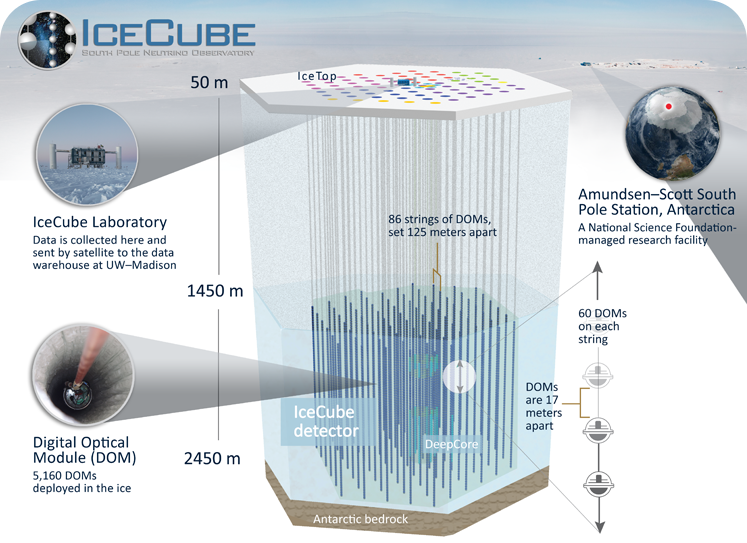
\includegraphics[width=\textwidth]{chapter5/img/icecube_detector_sm.png}
\caption{Illustration of the IceCube South Pole neutrino observatory.}
\label{fig:ICgeometry}
\end{figure} 

\begin{figure}
\centering
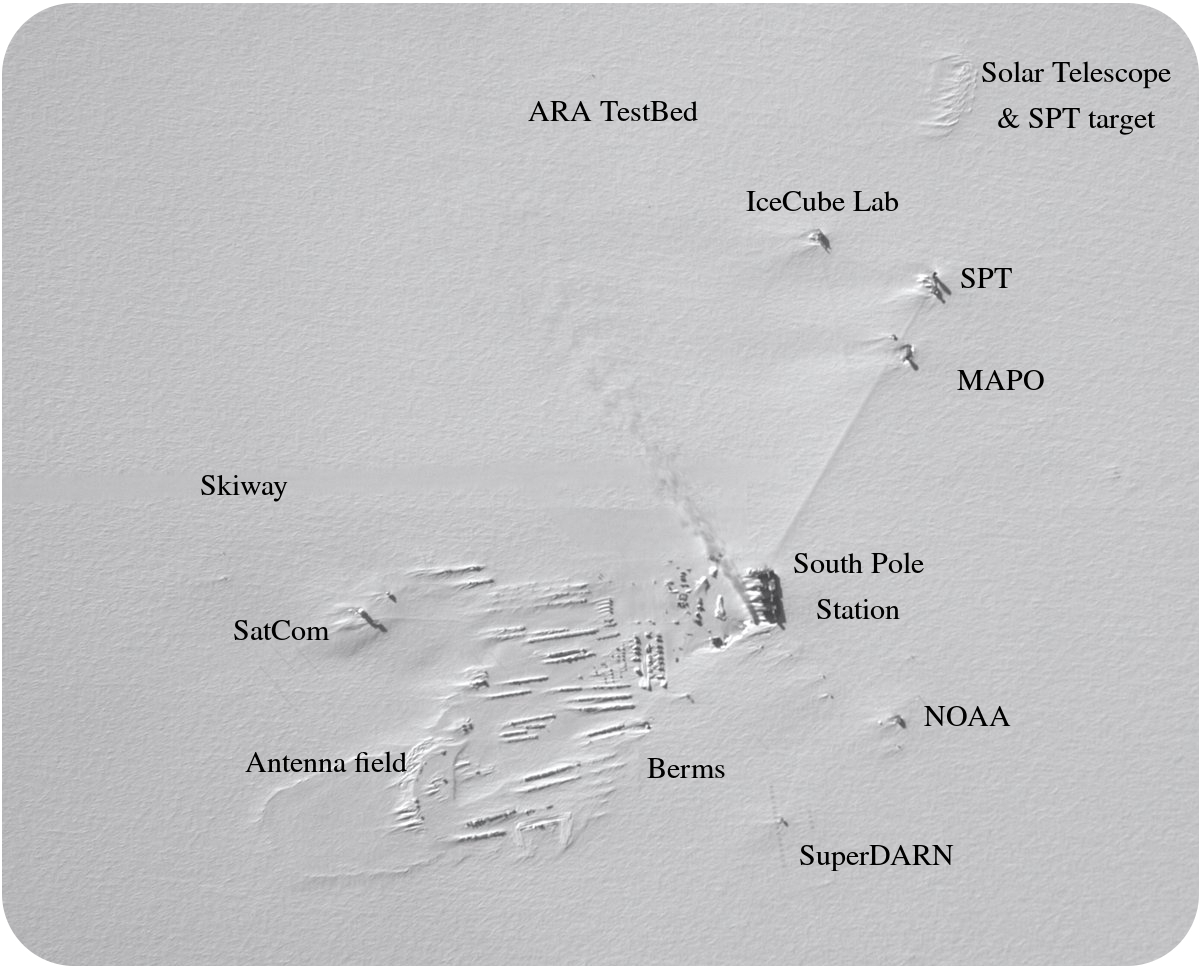
\includegraphics[width=0.75\textwidth]{chapter5/img/SouthPole_3.jpg}
\caption{Aerial view of the South Pole. The main buildings and experimental setups are indicated in the figure. The exhaust of the South Pole Station is also visible.}
\label{fig:aerialview}
\end{figure} 

\section{Geometry}
The IceCube detector consists of three main parts that act as different purpose physics detectors. 
The \textit{in-ice IceCube} detector is the main component and consists of 4680 digital optical modules. In its core, a denser subdetector, \textit{DeepCore}, significantly enhances the capabilities for low-energy events of the observatory in a limited volume. The center of the DeepCore array consists of 480 sensors.
On the surface of the ice, water tanks with optical modules inside are spread out over an area of approximately 1 km$^2$ and make up the \textit{IceTop detector}. This surface array was built as a cosmic ray detector and veto for the in-ice array.  The three components combined make the facility a multipurpose physics detector. Figure \ref{fig:ICgeometry} shows the layout of the detector.

\subsection{In-ice array}
The in-ice array consists of 4680 digital optical modules (DOMs) that are able to register light that is scattered and propagated through the ice (more info about these modules can be found in Section \ref{subsec:doms}). The DOMs are attached to cables and are frozen in the ice. In total, 78 of these ``strings'' were frozen into boreholes and spread out over a cubic kilometer in a hexagonal shape. Because only the deep ice is transparent, the DOMs are attached to the strings starting from a depth of 1450 meters to 2450 meters. The strings, as viewed from above, are spaced about 125 meters apart and along each string, 60 DOMs are attached with a vertical separation of 17 meters. This design was chosen in order to meet the primary science requirement of detecting astrophysical neutrinos in the energy range of $\mathcal{O}$(TeV)– $\mathcal{O}$(PeV).

 
\subsection{DeepCore}
\label{subsec:DC}
A subset of in-ice DOMs is deployed along eight extra strings in the central region of the in-ice array. The optical modules are deployed deeper than 1750 meter with a denser instrumented volume. Seven additional strings, belonging to the standard in-ice strings, are also combined with the DeepCore strings to optimize the instrumented volume for this detector. The inter-string spacing on the eight specialized DeepCore strings varies from 41 meters to 105 meters. The DOM-to-DOM spacing is 7 meters for the bottom 50 optical modules (which are deployed at depths of 2100 to 2450 meters). The remaining 10 DOMs on each string are located at depths above 2000 meters deep with a spacing of 10 meters. This extra ``layer'' serves as a veto for downgoing atmospheric muons. Each string is instrumented with 60 DOMs, resulting in a total of 480 DOMs. Instrumentation in the ice between 2000 to 2100 meters proved to be less useful due to the \textit{dust layer} (see Section \ref{sec:ice}) and was therefore left out. Six out of the eight specialized strings are also instrumented with DOMs using PMTs of higher quantum efficiency. The two remaining strings are instrumented with regular IceCube DOMs. A layout of the in-ice array is given in Figure \ref{fig:layoutIC}.

The DeepCore design allows us to detect neutrinos of much lower energies in the range of $\mathcal{O}$(10 GeV)– $\mathcal{O}$(100 GeV). Experiments for neutrino oscillation experiments, WIMP dark matter annihilation, galactic supernova neutrinos and point sources are made possible, or more feasible, with this dense subarray \cite{Collaboration:2011ym}.

\begin{figure}[t]
\centering
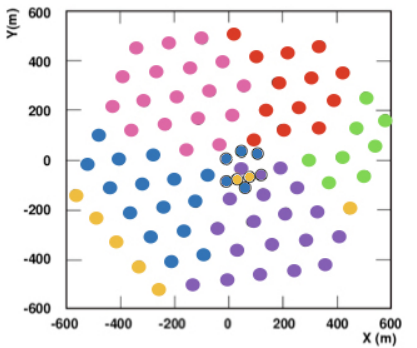
\includegraphics[width=0.5\textwidth]{chapter5/img/layoutIC.png}
\caption{Layout of the IceCube (regular) and DeepCore strings (black edge). The string color scheme represents different deployment seasons (04-05: orange, 05-06: green, 06-07: red, 07-08: pink, 08-09: purple, 09-10: blue, 10-11: yellow). Figure from Ref. \cite{Choma:2018zbe}, with minor corrections.}
\label{fig:layoutIC}
\end{figure}

\subsection{IceTop}
IceTop is a cosmic ray air shower array, located on the surface of the ice and 2835 meters above sea level. As discussed in Chapter \ref{ch:cr}, air showers die out when they are propagating to Earth's surface but as a consequence of the high altitude of IceTop, showers are observed near maximum\footnote{The height of the shower where the maximum number of particles are produced in an air shower is often referred to as the ``shower maximum''.}, resulting in a good energy resolution for the detector. This is important if one wants to measure changes in composition as a function of energy. In total, 162 ice-filled tanks are distributed in 81 stations (two tanks per station) in a grid similar to the in-ice array. Like the denser DeepCore infill, there are eight stations in the center of IceTop placed more closely together. 

The two tanks per station are separated 10 meters apart from each other and each tank contains two IceCube DOMs. One is operated at a ``low-gain'' and one at ``high-gain'', making them more suitable for air shower detection. The tanks measure the Cherenkov light that is produced in the ice of a tank due to the particles in a shower (electrons, positrons, muons, gamma rays and hadrons). The IceTop design allows to fully cover the knee of the energy spectrum and is primarily sensitive from PeV to EeV energies. The denser infill allows the threshold to be lowered to 100 TeV. The detector is used in studies of the composition, high-$p_T$ muons, etc. 

\subsection{IceCube coordinate system}
When referring to positions and directions, one has to define a coordinate system that is be able to uniquely define these variables. The system used in the IceCube collaboration is shown in Figure \ref{fig:coordinates}.\\

\begin{figure}[t]
\centering
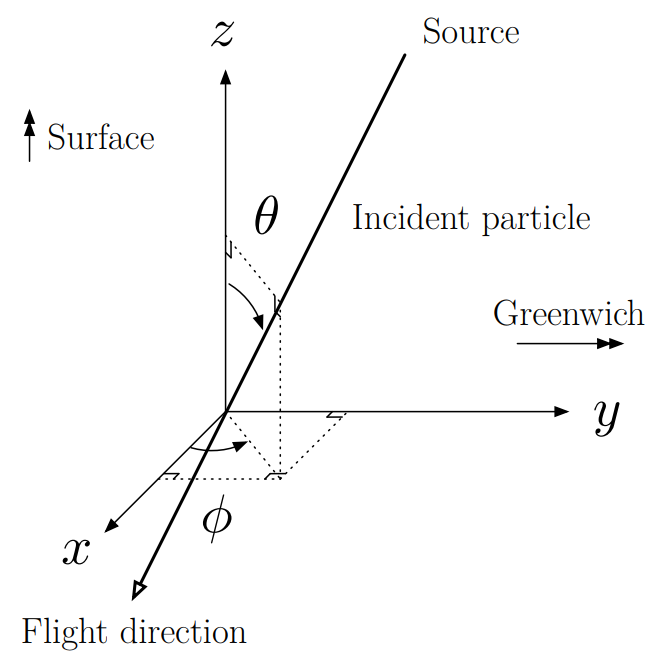
\includegraphics[width=0.5\textwidth]{chapter7/img/CoordinateSystem.png}
\caption{The IceCube coordinate system.}
\label{fig:coordinates}
\end{figure}

\noindent The center of the coordinate system is set close to the geometric center of the detector, at about 2000 m below the surface of the ice. The y-axis of the coordinate system is aligned with the Prime Meridian pointing toward Greenwich (United Kingdom). The x-axis is set perpendicular to the y-axis pointing in a, 90$^\circ$ clockwise direction. The z-axis is set perpendicular to the xy-plane, pointing upwards, normal to the Earth's surface.

A particle's direction is defined with zenith and azimuth angles, $\theta$ and $\phi$ respectively. The zenith angle is measured relative to the positive z-axis and the azimuth angle is measured counterclockwise from the positive xy-plane.



\section{Hardware components}
\subsection{Digital optical modules}
\label{subsec:doms}
The Digital Optical Modules, or DOMs, convert light into electrical signals and have the necessary hardware installed to perform some basic processing of the electrical pulses. A downward facing 10''-diameter photomultiplier tube (PMT) is set with a high voltage of 2 kV, resulting in a gain of $10^7$ \cite{Aartsen:2016nxy}. The amplitude of the resulting waveforms ranges from 1 mV up to and beyond the linearity limit of the PMT ($\sim2$ V) with the width ranging from 12 ns to 1500 ns. This wide dynamic range of the waveform is processed by onboard electronics: the main board and delay board. The main board controls all the devices in the DOM (high voltage power supply for the PMT, the flasher board and pressure, temperature, and power supply voltage monitor sensors), digitizes the PMT waveforms, communicates with the data acquisition (DAQ) on the surface, houses an internal clock that is regularly calibrated with the DAQ on the surface and exchanges pulses with the adjacent DOMs.
An illustration of the mechanical components of the optical module and a schematic view of the data flow starting from the PMT is shown in Figure \ref{fig:DOM}. The optical module is housed in a 13''-glass sphere of 0.5'' thick made from borosilicate. It is separated into two halves and held together with an aluminium waistband. The sphere was tested up to 690 bar hydrostatic pressure and is able to withstand the enormous pressure that the DOM is exposed to deep within the ice and during freezing (see Section \ref{sec:deployment}). A penetrator inside the glass sphere brings out three wire pairs housed in a cable. One wire pair is connected to the string and ultimately to the IceCube Laboratory (see Section \ref{subsec:icl}). The other two wires are connected to the neighboring DOMs directly above and below for local coincidence pulses (see Section \ref{subsec:cablesystems}). A detailed description is given in the detector paper \cite{Aartsen:2016nxy}.

\begin{figure}
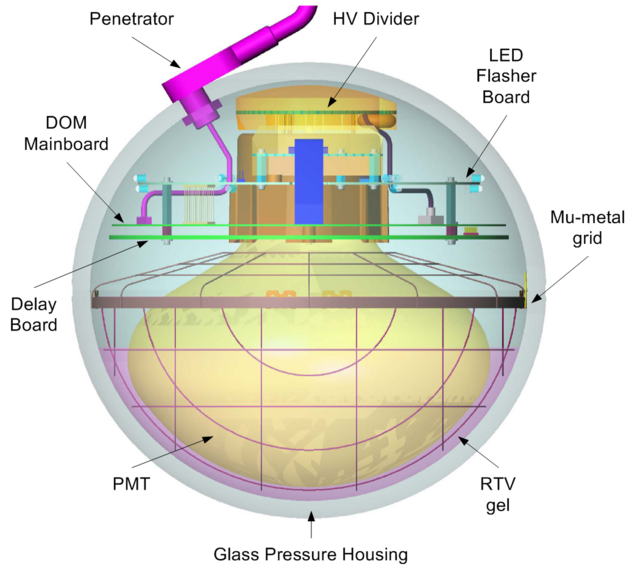
\includegraphics[width=0.48\textwidth]{chapter5/img/DOM-Picture.png}
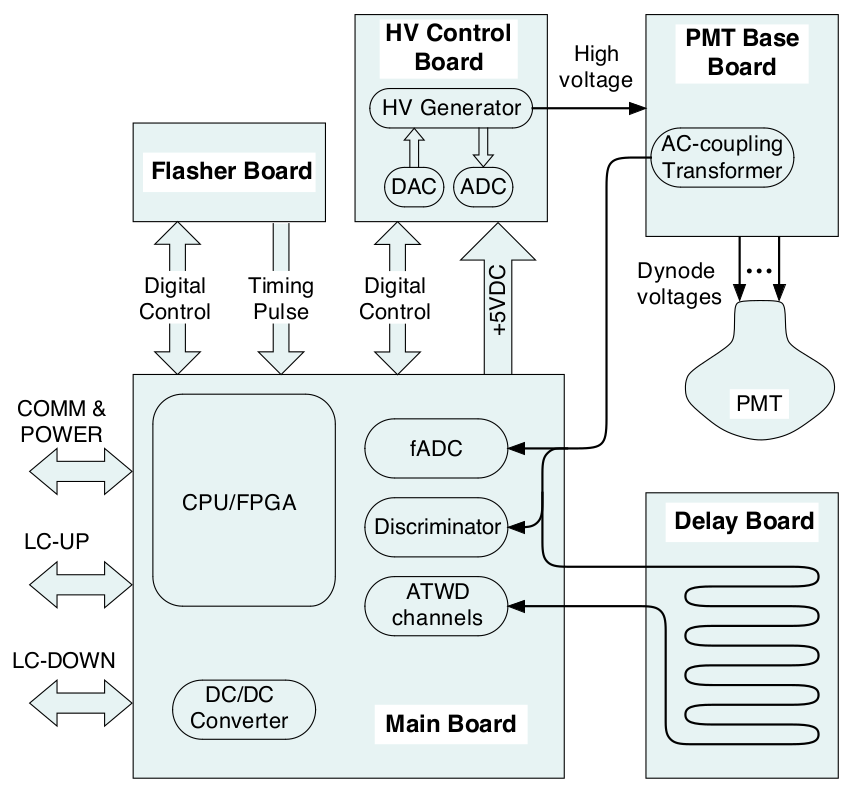
\includegraphics[width=0.48\textwidth]{chapter5/img/electronicsDOM.png}
\caption{\textit{Left:} illustration of the mechanical DOM components. \textit{Right}: Scheme of the functional connections.}
\label{fig:DOM}
\end{figure}

\subsubsection{PMTs}
The 10'' (or 25 cm) diameter PMT comes in two types: Hamamatsu R7081-02 for standard IceCube DOMs and a high-quantum-efficiency (HQE) version, Hamamatsu R7081-02MOD for the specialized DeepCore strings \cite{Abbasi:2010vc}. The peak quantum efficiency is around 25\% (34\% for HQE) at a wavelength of approximately 390 nm. However, the total acceptance of the optical module is the convolution of the quantum efficiency with the glass transmission (93\% at 400 nm, decreasing to 50\% at 340 nm and 10\% at 315 nm at a normal incidence). The resulting acceptance is illustrated in Figure \ref{fig:acceptance}. The PMTs face downwards and are housed in a mu-metal grid to shield them from the Earth magnetic field and a silicone gel necessary for optical coupling and mechanical support.

\begin{figure}[t]
\centering
\includegraphics[width=0.7\textwidth]{chapter5/img/acceptanceDOM.png}
\caption{Fraction of photons arriving from a direction parallel to the PMT axis and are recorded in function of the photon wavelength. Glass and gel transmission, PMT quantum and collection efficiencies are all included. Figure from Ref. \cite{Aartsen:2013rt}.}
\label{fig:acceptance}
\end{figure}


\subsubsection{Main board and delay board}
\label{subsec:mainboard}
The PMT signals are sent to two ATWDs (Analog Transient Waveform Digitizer) and one fast ADC (fADC) with a delay of about 75 ns. This delay is necessary because signals are only processed if the signal exceeds a voltage that corresponds to 0.25 PE (one PE is the voltage that typically corresponds to the voltage produced by a single photoelectron). The delay board consists of a 10 m-long copper trace that delays the signal for 75 ns, necessary to be able to record the full waveform before the discriminator threshold of 0.25 PE is exceeded. 

Once this threshold is crossed, the signal is compressed and included in a ``DOMlaunch'' or ``hit''. Signals that pass the local coincidence requirement (see Section \ref{subsec:cablesystems}) have their full waveforms compressed, whereas for isolated events only a time stamp and brief charge summary is sent. For each hit, an FPGA  (Field Programmable Gate Array) opens up one of the two ATWD chips. Each of the two chips is provided with three amplifier gains with nominal values of 16, 2 and 0.25. Most pulses use the highest-gain channel while the other lower-gain recordings are used as needed when pulses reach 75\% of the range of a higher-gain channel. The ATWD recording duration is 427 ns, which should include light that is produced within tens of meters of a DOM. The slower fADC is used when light reaches the DOM after the ATWD time window and samples continuously. The FPGA is programmed to save an interval of 6.4 $\mu$s after the launch. ATWD chips sample the input voltage at 300 Msps, followed by a 10-bit digitization. The fADC captures the information with a 10-bit 40 Msps.

The two sets of ATWD chips are operated alternately in order to reduce deadtime. After 50 ns, the second chip is available to be launched during the digitization step of the first. The digitization procedure is terminated for isolated hits and the ATWD is reset, reducing the DOM dead time.\\


\subsubsection{Flasher board}
\label{subsub:flasher}
To be able to characterize the ice and simulate light propagation, each DOM was instrumented with 12 LEDs that are aimed in six different azimuth angles (with 60$^\circ$ spacing) and along two different zenith angles. The LEDs were chosen to have a wavelength spectrum centered at around 400 nm to approximate the typical wavelength of detected Cherenkov photons. Flasher data is used for:
\vspace{2mm}
\begin{itemize}
\item verifying the timing response of the DOMs throughout the analysis software chain;
\item measuring the position of the deployed DOMs in ice;
\item measuring the optical properties of the ice (see Section \ref{sec:ice});
\item verifying the performance of shower reconstruction algorithms in measuring position, direction and energy.
\end{itemize}



\subsection{Calibration}
\label{subsec:calibration}
Regular calibration of the components is necessary to be able to convert the DOM waveforms to reliable and comparable physical units. Optical efficiencies of the optical modules were determined in the lab before deployment and are also measured \textit{in situ} with calibration procedures.

Some of these procedures do not allow for simultaneous data-taking and are performed as little as possible, without losing significant confidence in the calibration of the devices. For example, in-ice DOMs are calibrated yearly with the DOMCal procedure, whereas global time calibration can be done in parallel with data-taking and is provided by the RAPCal procedure.

As they result in the vast majority of the background hits, \textit{dark noise} needs to be properly understood for low-energy neutrino analyses, supernova searches, and detector simulations. The total rate of dark noise averages at around 560 Hz for in-ice DOMs and 780 Hz for HQE DOMs. The origins of the noise are non-trivial and include electronic noise, thermionic emission, Cherenkov light from radioactive decays, field emission within the PMT, and scintillation/luminescence in the glass of the PMT and pressure sphere. They are simulated with a combination of uncorrelated (Poissonian) noise and a correlated component. The temperature dependence of the noise rate was determined by combining a measured temperature profile of the South Pole ice cap with a fit of the Poissonian expectation of the total dark noise rate to every individual DOM, and was verified in lab measurements. The seasonal variations of the dark noise rates are below 1\%, but are tracked over time and updated yearly in a database.\\

\noindent More information about these and other calibration procedures can be found in Ref. \cite{Aartsen:2016nxy}.

\subsection{Cable systems}
\label{subsec:cablesystems}
\begin{figure}
\centering
\includegraphics[width=0.9\textwidth]{chapter5/img/cablelayout.png}
\includegraphics[width=0.9\textwidth]{chapter5/img/cableSchematic_withcable.png}
\caption{\textit{Top}: Sketch of DOM cabling and schematic overview. The modules are connected to their nearest neighbors and the string. \textit{Bottom}: General schematic overview of the IceCube cabling system and the connection between all components together with an in-ice cable cross section. Illustrations from Ref. \cite{Aartsen:2016nxy}.}
\label{fig:cable}
\end{figure}

The DOMs are the eyes of the detector, but the cable system connects all the modules together and links them to the readout hardware at the surface. The in-ice cables, 2505 m long, are each connected to 60 DOMs and terminate at a Surface Junction Box (SJB) between IceTop tanks. IceTop tanks also connect to the SJB. A surface cable was trenched 1 m deep at the time of deployment and runs to the IceCube Laboratory. One cable consists of 20 ``quads'', a construction of four twisted wires. Four quads provide special instrumentation and local coincidence between connections and one is a spare. The remaining 15 quads are each connected to four DOMs with two wire pairs. A wire pair connects two adjacent DOMs and is attached to connectors at 30 breakouts spaced 34 m apart as can be seen in Figure \ref{fig:cable}. Each DOM is connected to three wire pairs. One wire pair is used for bi-directional communication to the surface and power. The two remaining wires are dedicated to determine \textit{Local Coincidence (LC)}. Each DOM is connected to its nearest neighbor above and below. If nearest or next-to-nearest neighbors are hit within a time window of $\pm$ 1 $\mu$s, the hits are said to be in Hard Local Coincidence (HLC). Isolated hits are referred to as Soft Local Coincidence (SLC). Most DOM hits originate from dark noise (see Section \ref{subsec:calibration}) and are not in HLC. Light originating from particles traveling through matter is more likely to trigger DOMs in close proximity. Therefore, LC requirements are able to drastically reduce the noise rate.

\subsection{IceCube laboratory}
\label{subsec:icl}
The central building to which the modules of all the detectors are connected is the IceCube Laboratory (ICL). Cables/strings from the arrays run up two cable towers on either sides of the structure. A picture of the ICL is shown as the header image of this chapter (pg. \pageref{ch:icecube}); one of the towers is visible. Inside the main part of the building is a server room to which the cables in the towers are connected. All data acquisition and online filtering computers are housed inside the server room together with the main IceCube computing system called the ``South Pole System'' (more information on this in Section \ref{sec:datataking}).


\section{Deployment}
\label{sec:deployment}
In total, 86 holes had to be drilled for all IceCube and DeepCore strings. The surface consists of a 50 m snow and firn region with a gradual transition to ice. The ice was melted with a 5 MW Enhanced Hot Water Drill (EHWD) capable of drilling about 1 hole per 48 hours. The holes were 60 cm in diameter, providing enough clearance for the optical modules that were 35 cm in diameter, and with contingency time for delays that meant holes could shrink due to refreezing. Because melting snow and firn with hot water is not practical, a specialized drill with copper tubing through which hot water flows was used to melt the firn by contact.

The IceCube drilling was completed in seven field seasons during Antarctic summers (early November to mid-January). The first season started in 2004-2005 and construction ended in 2010-2011. 
%At the end of each season, the Seasonal Equipment Site (SES) that provided electricity and a stable supply of hot pressurized water had to be decommissioned and positioned at the site for the next drilling season due to its size and complexity. From the SES a more flexible Tower Operations Site (TOS) was linked and held the drill tower, operations building, and hose and cable reels. There were two towers, where one was set up for drilling while the second one was still being used for deployment of the cables.

After drilling one hole, all 60 DOMs were lowered one by one and connected to each other with the penetrator assembly as shown in Figure \ref{fig:cable}. After deployment of all DOMs, the remaining 1,\.5 km of in-ice cable was lowered into the hole (known as the ``drop phase''). The top of the cable was then secured by an anchor trenched in the snow and connected to the Surface Junction Box. 

In total, 5484 (5160 IC + 324 IT) optical modules were deployed and as of 2018, there are 5396 still in data-taking mode (98.4\%). There were 55 DOMs that failed almost immediately during freeze-in, while 34 DOM failures occurred after deployment. This number includes modules on a wire pair that are taken out when the partner DOM on the same pair failed. The mean failure rate is estimated to be around $(4.1 \pm 1.2)$ yr$^{-1}$, which results in a survival fraction of $(97.4 \pm 0.3)\%$ in 2030.

\section{Data taking}
\label{sec:datataking}

\begin{figure}[t]
\centering
\includegraphics[width=0.7\textwidth]{chapter5/img/dataflow.png}
\caption{Schematic overview of the data flow in the primary IceCube online systems.}
\label{fig:dataflow}
\end{figure}
First processing of the photon detection is done inside the DOM as mentioned in Section \ref{subsec:mainboard}. After digitization, the waveforms are sent along the cable/string to which all DOMs are attached and that runs to the ICL. Each one of the strings is connected to one of the DOMHubs, which together with servers that run various online systems, comprises the South Pole System (SPS). An overview is given in Figure \ref{fig:dataflow}.

The data acquisition (DAQ) system is run on the DOMHubs and recognizes patterns in hits that are most likely caused by particle interactions with the use of the implemented triggers and filters (see below). This combination of hits is called an ``event''. Most of the DAQ data rate originates from atmospheric muons with an event rate averaging 2.7 kHz. The total bandwidth saved to tape/disk (see Section \ref{subsec:datahandling}) is approximately 1 TB/day.

To implement possible changes in the detector settings, triggers, or filters, a full physics run spans over one year, starting in May and ending in May the following year. Data is recorded in smaller 8 hour runs, where each run has a unique run number. Over the years, with the use of both online and on-site automatic alerts, the total uptime of the detector has a steady increase of clean uptime (usable data) from 89.75\% in 2011 to 98.89\% in 2018.

\subsection{Triggers}
\label{subsec:triggers}
Aside from the discriminator thresholds in the module (see Section \ref{subsec:mainboard}), a system of triggers is set up to further reduce the noise rate and refine searches for physics events. Below, a short description of the triggers is given. An overview of the trigger settings is given in Table \ref{tab:trigger}. 

\vspace{2mm}
\begin{itemize}
\item The most important trigger is the Simple Multiplicity Trigger (SMT) used for the IceCube, DeepCore and IceTop arrays. The trigger setting requires a certain number of HLC hits within a time window of the order of a couple of $\mu$s without any locality requirements.
\item The Volume Trigger requires less HLC hits, but they have to be clustered in a certain cylindrical volume. 
\item Locality conditions are powerful for low-energy events that do not reach far in the detector but are more prone to produce hits in a small volume and time window. Therefore, a dedicated String Trigger was designed for low-energetic upgoing events passing along a single string. 
\item IceCube is also sensitive to hypothetical massive particles moving at subrelativistic speeds: magnetic monopoles. Therefore, a dedicated Slow Particle (SLOP) trigger has been developed. It searches for triplets of HLC pairs within a window, $T_{\textrm{max}}$, and removes HLC pairs within a time window, $T_{\textrm{prox}}$, to remove hits originating from particles traveling at the speed of light. Other velocity and geometric requirements are set with the inner angle between triplets, $\alpha_{\textrm{min}}$ and the ``velocity'' along the sides of the triangle.
\item A Fixed Rate Trigger (FRT) reads out hit data from the full detector at fixed intervals, useful for DOM noise studies.
\end{itemize}
\vspace{2mm}

\noindent If a trigger condition is fulfilled, the start of the trigger window is determined as the first HLC hit of the active volume of the trigger. The minimum length of the triggered window slides along with the hits until there is no more HLC after the last hit within the set minimum time window. The length of a triggered set of hits can therefore be longer than the minimum trigger window. As one event is able to fulfill multiple trigger requirements, the (sub)triggers are merged into one Global Trigger while keeping the information on the individual triggers. This data is subsequently sent to the Event Builder that writes DAQ events (also called \textit{Q frames}) to a temporary file that is saved when it reaches a certain size. These events are eventually re-split into physics events (\textit{P frames}) corresponding to a certain subtrigger before reconstruction and analysis. An example of a Global Trigger, here mostly determined by the very long SLOP trigger, is shown in Figure \ref{fig:globaltrigger}.

All triggers read out all SLC/HLC hits of all DOMs, even the ones not directly involved in the trigger construction. For this, they use the StringHub software component located on every DOMHub that is able of caching SLC and HLC hits in memory. Hits before and after the trigger window are also saved to the event to add information of early and late pulses. This is typically 4 $\mu$s before and 6 $\mu$s after the trigger window for in-ice triggers. 



%The StringHub is also able to save local ``HitSpool'' on-disc data and later request it if necessary from the Event Builder. This HitSpool data is able to store up to 16 hours of all waveforms overwriting the oldest data first and originally intended for the detection of Galactic supernovae. Such an event would give rise to a steady increase in apparent dark noise from its low-energy neutrinos without fulfilling the standard trigger requirements. Over the years, the HitSpool data has found multiple other usecases such as a neutron echo analysis, searching for delayed neutrons from hadronic interactions \cite{Aartsen:2017mnf}. 

\begin{figure}[t]
\centering
\includegraphics[width=0.8\textwidth]{chapter5/img/globaltrigger.png}
\caption{Example of a global trigger construction. Multiple triggers are combined due to their overlap with the long SLOP trigger.}
\label{fig:globaltrigger}
\end{figure}


\begin{table}[]
\centering
\caption{Parameter settings of triggers (as of May 2016) and typical trigger rates.}
\label{tab:trigger}
\resizebox{\textwidth}{!}{%
\begin{tabular}{|l|r|r|r|c|c|r|r|}
\hline
\cellcolor[HTML]{F1A91E} & \multicolumn{1}{c|}{\cellcolor[HTML]{F1A91E}} & \multicolumn{1}{c|}{\cellcolor[HTML]{F1A91E}} & \multicolumn{1}{c|}{\cellcolor[HTML]{F1A91E}} & \multicolumn{2}{c|}{\cellcolor[HTML]{F1A91E}Readout Window ($\mu$s)} & \multicolumn{1}{c|}{\cellcolor[HTML]{F1A91E}} & \multicolumn{1}{c|}{\cellcolor[HTML]{F1A91E}} \\ \cline{5-6}
\multirow{-2}{*}{\cellcolor[HTML]{F1A91E}Trigger} & \multicolumn{1}{c|}{\multirow{-2}{*}{\cellcolor[HTML]{F1A91E}DOM set}} & \multicolumn{1}{c|}{\multirow{-2}{*}{\cellcolor[HTML]{F1A91E}$N$ HLC hits}} & \multicolumn{1}{c|}{\multirow{-2}{*}{\cellcolor[HTML]{F1A91E}Trigger Window ($\mu$s)}} & \multicolumn{1}{c|}{\cellcolor[HTML]{F1A91E}\ \ \ \ IC\ \ \ \ } & \multicolumn{1}{c|}{\cellcolor[HTML]{F1A91E}\ \ \ \ IT \ \ \ \ } & \multicolumn{1}{c|}{\multirow{-2}{*}{\cellcolor[HTML]{F1A91E}Topology}} & \multicolumn{1}{c|}{\multirow{-2}{*}{\cellcolor[HTML]{F1A91E}Rate (Hz)}} \\ \hline
\textbf{SMT} & \textbf{in-ice} & 8 & 5 & $-4,+6$ & $\pm10$ & - & 2100 \\ \hline
\textbf{SMT} & \textbf{DeepCore} & 3 & 2.5 & $-4,+6$ & $\pm10$ & - & 250 \\ \hline
SMT & IceTop & 6 & 5 & $\pm10$ & $\pm10$ & - & 25 \\ \hline
\textbf{Volume} & \textbf{in-ice} & 4 & 1 & $-4,+6$ & $\pm10$ & cylinder (r = 175 m, h = 75 m) & 3700 \\ \hline
Volume & IceTop & 4 & 0.2 & $\pm10$ & $\pm10$ & cylinder (r = 60 m, h = 10 m) & 4 \\ \hline
\textbf{String} & \textbf{in-ice} & 5 & 1.5 & $-4,+6$ & $\pm10$ & 7 adjacent vertical DOMs & 2200 \\ \hline
 &  &  & $T_{\textrm{prox}} = 2.5$ &  &  &  &  \\ \cline{4-4}
 &  &  & $T_{\textrm{min}} = 0$ &  &  &  &  \\ \cline{4-4}
\multirow{-3}{*}{SLOP} & \multirow{-3}{*}{in-ice} & \multirow{-3}{*}{$N_{\textrm{triplet}}$} & $T_{\textrm{max}} = 500$ & \multirow{-3}{*}{$-4,+6$} & \multirow{-3}{*}{$\pm10$} & \multirow{-3}{*}{$\alpha_{\textrm{min}} = 140^\circ, v^{\textrm{max}}_{\textrm{rel}} = 0.5$} & \multirow{-3}{*}{12} \\ \hline
FRT & all & - & - &  \multicolumn{2}{c|}{Combined: 10000} & - & 0.003 \\ \hline
\end{tabular}%
}
\end{table}



\subsection{Filters}
\label{subsec:filters}
Events are sent through the online Processing and Filtering (PnF) system for additional processing. First, the triggered events have their waveforms further compressed using the Super Data Storage and Transfer format (SuperDST), which uses only 9\% of the storage size of the full waveform information. Very fast, basic reconstructions are run on the SuperDST waveforms to compute the vertex position, energy, direction and goodness-of-fit that are necessary for the filter selections of possible interesting events.

Around 25 filters search for a wide range of different types of particle interactions, ranging from low-energy neutrinos for oscillation measurements to the highest-energy neutrino interactions illuminating large parts of the detector. Some filters are designed to look for neutrino events of wide astrophysical interest to the scientific community and trigger alerts that are distributed to followup observatories worldwide. One example is the ``EHE alert'' that searches for Extremely High Energy neutrinos that are most likely of astrophysical origin \cite{Aartsen:2016lmt}. Another example is the Gamma Follow Up alert that notifies the MAGIC and VERITAS collaborations when significant bursts of neutrinos from known high-energy gamma-ray sources over periods up to 3 weeks occur \cite{1412973}. Other filters look for events that could be caused by muons, WIMPs, monopoles, etc. The filters that were used in this analysis are given in Section \ref{sec:filterselection}.

As a bonus, filtering reduces the data volume to a level of around 90 Gb/day, which is small enough to transfer to the North using a satellite.

\subsection{Data handling}
\label{subsec:datahandling}
Most of the data is processed with the PnF system. The geometry, calibration, and detector status (GCD) information from each 8 hour run is sent via the same satellite transfer that is used for the continuously running PnF system. All the raw waveforms were written to tape before that system was retired in 2015. Since then, disks have been used to store the remaining archival data. This raw data is shipped to the North every year and is used if reprocessing of data is necessary. An example is the SPE correction for all runs starting from 2010 to 2016 referred to as \textit{pass2 data} \cite{pass2}. \\

\noindent Events are stored in IceCube specific files and are called \textit{i3files} \index{i3file}.

\section{IceCube event topology}
The compressed waveforms are refolded to approximations of the original waveforms using average single-photoelectron pulse shapes as can be seen in Figure \ref{fig:waveform}. The timing, shape and amplitude of the reconstructed waveforms in all the DOMs in an event are used to characterize the event topologies in the detector. Different interactions give rise to several possible signatures in the detector. Energetic muons propagate several hundreds of meters in the ice and give rise to tracks, whereas electrons and hadrons are stopped almost immediately, giving rise to cascades (see Section \ref{sec:propagation}).

\begin{figure}[t]
\centering
\includegraphics[width=\textwidth]{chapter5/img/waveform.png}
\caption{\textit{Left:} pulse information illustrated with blue bars; the leading-edges time, width, and charge of the pulse are given by the left edge, width, and height of the bar, respectively. The red bars show the same after SuperDST compression. \textit{Right: }Reconstructed pulses using the full pulse profiles in blue are compared to an approximation of the original waveform that is obtained by convolving the pulse times and charges with an average single-photoelectron pulse shape. Figures from Ref. \cite{waveforms}.}
\label{fig:waveform}
\end{figure}

The track-like events, originating from charged-current muon neutrino interactions, provide an angular resolution at a typical angle of 1$^\circ$ for well-contained and reconstructed tracks at 1 TeV and improves to $\sim 0.3^\circ$ for neutrinos with an energy of 1 PeV \cite{Aartsen:2018ywr}. Cascades, originating from electromagnetic or hadronic cascades, result in a more spherical light generation in the detector. Well-contained shower events have an average deposited energy resolution of around 15\%. These event types are shown in more detail in Figure \ref{fig:ICinteractions2}.
 

\begin{figure}
\centering
\includegraphics[width=\textwidth]{chapter4/img/ICinteractions2.png}
\caption{Neutrino interactions in the IceCube detector have two distinct types of interactions: cascades and tracks. Energetic taus are theorized to have double-bang signatures but have not undeniably been seen. Colors determine the timing of hits in the optical modules in the ice. Illustrations from the IceCube collaboration \cite{kjeroSignatures}.}
\label{fig:ICinteractions2}
\end{figure}



\section{Antarctic ice}
\label{sec:ice}
The ice, in which the optical modules are frozen, acts as the propagation medium for the light that is produced by relativistic particles. Therefore, the parameterization of the ice is of great importance for good reconstructions and reliable simulations. The relativistic particles that travel through the ice produce photons in a Cherenkov cone with an opening angle of around 41$^\circ$ (see Section \ref{sec:cherenkoveffect}). How these photons further propagate from the point of emission to the receiving sensors is determined by the absorption and scattering within the ice. The most important parameters necessary to describe the photon propagation in ice are:
\vspace{2mm}
\begin{itemize}
\item the average distance to absorption,
\item the average distance between successive scatters of photons, and 
\item the angular distribution of the new direction of a photon at each given scattering point.
\end{itemize}
\vspace{2mm}
There has been a large effort into measuring and modeling the Antarctic ice that is still ongoing. A good summary (although is a bit outdated as it does not include ice anisotropy effects, cable shadowing and DOM tilts) can be found in Ref. \cite{Aartsen:2013rt}.

\subsection{Ice simulation}
\label{subsec:icesimulation}
The ice is modeled by the six-parameter ice model introduced in Ref. \cite{Ackermann:2006pva}. Flasher data from LEDs is used to fit the model to data (see Section  \ref{subsub:flasher}). In this model, the ice is described by a table of depth-dependent parameters $b_e(400)$ and $a_{dust}(400)$ related to scattering and absorption at a wavelength of 400 nm. These two parameters depend on the relative temperature $\delta \tau$, which changes in function of depth, and six global parameters. The effective scattering coefficient is equal to $b_e = b \cdot \left( 1-\langle \cos \theta \rangle \right)$, where $b$ is the geometrical scattering coefficient that determines the average distance between successive scatters and $\theta$ is the deflection angle at each scatter. The absorption coefficient $a$ determines the average distance traveled by a photon before it is absorbed and is the sum of two components: one due to dust and the other a temperature dependent component for pure ice.

\begin{equation}
b_e(\lambda)  = b_e(400) \cdot \left( \frac{\lambda}{400}\right)^{-\alpha},
\end{equation}

\begin{equation}
\begin{split}
a(\lambda) &= a_{dust}(\lambda) + A e^{-B/\lambda} \cdot (1+0.01 \cdot \delta \tau), \\
&\textrm{with} \ \ \ a_{dust}(\lambda) = a_{dust}(400) \cdot \left( \frac{\lambda}{400}\right)^{-\kappa}.
\end{split}
\end{equation}
$\alpha, \kappa, A \textrm{ and } B$ are determined in Ref. \cite{Ackermann:2006pva}\footnote{The remaining two parameters $D$ and $E$ were not used here.}, $\delta \tau$ is equal to

\begin{equation}
\begin{split}
&\delta \tau(d) = T(d) - T(1730 \textrm{m}), \\ 
\textrm{with} \ \ T(d) = 221.5 &- 0.00045319 \cdot d + 5.822 \cdot 10^{-6} \cdot d^2,
\end{split}
\end{equation}
where $d$ is the relative depth compared to the center of AMANDA (1730 m depth). Using flasher data with 400 nm wavelengths, it is possible to measure the values of $b_e(400)$ and $a_{dust}(400)$ at certain depths and use the six-parameter ice model to extrapolate scattering and absorption for other wavelengths. 

In 2008, a flasher run was launched where each DOM on string 63 was producing flashes. The layout of the detector at the time of the flasher run and results of fits to $b_{e}(400)$ and $a(400)$ vs. depth can be found in Figure \ref{fig:2008config}. At a depth between 2000 meters and 2100 meters, a large increase in scattering and absorption is clearly visible. A \textit{dust layer}, presumably originating from volcanic ash, is characterized by an increase of dust in the ice, responsible for the higher scattering and absorption factors.

\begin{figure}[t]
\begin{minipage}{6in}
  \centering
  \raisebox{-0.5\height}{\includegraphics[height=2in]{chapter5/img/2008config.png}}
  \hspace*{.7in}
  \raisebox{-0.5\height}{\includegraphics[height=3.5in]{chapter5/img/spiceleacoefficients.png}}
\end{minipage}
\caption{\textit{Left}: Top view of the 2008 detector configuration when DOMs on string 63 were used to flash LEDs in a flasher run. Same colors are used for strings located at a similar distance to the central string. \textit{Right}: values of $b_{e}(400)$ and $a(400)$ vs. depth for two different ice models. The scale and numbers to the right of each plot indicate the corresponding effective  absorption $1/a$ and scattering $1/b_e$ lengths in [m]. Both illustrations from Ref. \cite{1412998}.}
\stepcounter{figure}%
\label{fig:2008config}
\end{figure}

Over the years, multiple different ice models have been constructed. For this analysis the SPICELea\footnote{SPICE stands for South Pole Ice. Lea is an addition to distinguish the different model types, but has (as far as the author knows) no special meaning.} model has been set as nominal. This is the most recent model that has significant Monte Carlo background simulations available. It includes an angular sensitivity estimation due to the \textit{hole ice}, a column of ice approximately 30 cm in radius immediately surrounding the strings with an increased amount of scattering. More information about this model can be found in Ref. \cite{1412998}.
\subsection{Systematic uncertainties}
The characteristics of the ice are complex. Dust particles, the tilt in the ice sheets, etc. result into non-negligible uncertainties in the ice model. Data from the flasher runs are compared to simulation and this verification was used to quantify the uncertainty on the measured values of $b_e(400)$ and $a(400)$. From this, it was determined that $(+10\%,0), (0,+10\%)$ and $(-7.1\%,-7.1\%)$ uncertainties on the scattering and absorption coefficients, respectively, was a conservative estimation.



\section{Future upgrades}
The last couple of years there has been a large focus on improving the physics work that can be done in the IceCube experiment. Several projects are in the pipeline, are under R\&D, and/or have been funded to improve the full analysis case of the detector(s).

Lower-energy neutrinos can be detected with a denser infill with other optical modules (the Upgrade, see Section \ref{subsec:upgrade}), cosmic ray measurements can be improved with a complementary scintillator array to the IceTop tanks \cite{Collaboration:2017tdy} and small air Cherenkov telescopes \cite{Auffenberg:2017vwc}. Also, the detection of ultra-high-energy neutrinos could be made possible with a larger infill of the current IceCube in-ice array (Gen2) or radio antennas. Below a brief summary of projects that could be of potential importance to this analysis is given.

%\subsection{Scintillators}
%During the Antarctic summer of the 2017/2018 season, several scintillator prototypes were installed as proof-of-concept for a full scintillator\footnote{Scintillators collect light that is produced by particles travelling through matter that is excited by the relativistic particle (Bethe-Bloch formula).} array with a similar coverage of the current IceTop array. One station would consist of 7 scintillator panels; one as the center and the remaining six in a hexagonal shape around the center. A total of 37 stations result in 259 panels in total with an instrumented area of $\sim 388$ m$^2$ \cite{Collaboration:2017tdy}. This main purpose of this setup is twofold:
%\\
%\begin{itemize}
%\item \textbf{Measure the attenuation due to snow.} IceTop tanks suffer from snow accumulation and many IceTop analyses have this effect as their main systematic error. Electromagnetic components of air showers have short attenuation lengths in snow, resulting in a clear difference of signal rates for tanks that accumulated more snow than others in the course of the years since deployment. The uncertainty in the attenuation function, that depends on the distance to the shower axis, muon number, snow depth, energy, and zenith angle is expected to increase the estimated 6\% systematic uncertainty on the energy spectrum in the following years. A reference signal from the scintillators can reduce this systematic uncertainty.
%\item \textbf{Improve low-energy detection efficiency.} Scintillators are able to efficiently detect air showers to lower energies than currently possible with IceTop detectors only.
%\item \textbf{Signal determination.} The setup could also be used in a similar fashion as the Pierre Auger upgrade was used to distinguish the muon and electromagnetic contributions \cite{Aab:2016vlz}. 
%\end{itemize}
 
%\subsection{IceAct}
%The main backgrounds in most IceCube analysis (including the one described in this work) are from atmospheric muons and muon neutrinos. IceTop has been shown to act as a veto for these events and is used in some analyses \cite{Tosi:2017zho}. A possible complementary extension of the IceTop detector is based on small Air Cherenkov Telescopes (ACTs), called IceACT \cite{Auffenberg:2017vwc}. ACTs use air as the active volume for light production and use cameras to detect light produced by cosmic rays. Downgoing atmospheric neutrinos could be vetoed as they are also accompanied by air showers on the surface. Currently, several prototype setups are deployed and tested on South Pole. One prototype telescope consists of 61 pixel SiPM camera with a 60 mm focal plane radius as the central part. One station would consist of a central telescope with six others surrounding it in a hexagonal shape. Each telescope would be oriented to a different point in the sky, optimizing the total field of view. An array covering the IceTop and IceCube detectors is proposed but still being discussed. Stations further away could also be included to further optimize the veto capabilities and would include fewer than 7 telescopes as the detection of a very inclined cosmic ray with one telescope shields more modules deep in the ice than vertical cosmic ray events.

\subsection{IceCube Upgrade}
\label{subsec:upgrade}
\begin{figure}[t]
\centering
\includegraphics[width=0.8\textwidth]{chapter5/img/ICUpgradeLayout_V3.jpg}
\caption{Top view of the Upgrade infill (red circles) within the DeepCore array (green) and the whole IceCube detector (blue). The area of the circles is representative of the instrumented photocathode density on a given string. Illustration from the IceCube collaboration.}
\label{fig:upgrade}
\end{figure}

In 2018, a funding proposal for a dense 7-string infill of DeepCore was accepted by the NSF and was effective from the beginning of October later that year. This infill would have DOMs separated 2.4 m apart and start from a depth of 2140 m, reaching to 2440 m deep in the ice along seven new strings (see Figure \ref{fig:upgrade}). This very dense array would allow low-energy and oscillation experiments to reach much better sensitivities. Also, very dim tracks such as the ones from particles with an anomalous charge lower than $e$, might be easier to distinguish from low-energy muons that produce more Cherenkov light. 

Because this project involves a restart of the drill, it also serves as a testbed for new optical modules. The Upgrade is the first step towards the much bigger Gen2 project. New types of optical modules would be used with higher angular acceptances than the currently used DOMs that have one large downward facing PMT. Examples are D-Eggs, which have two PMTs at each end of an ellipsoid glass \cite{Ishihara:2017vxn}, and mDOMs, where multiple smaller PMTs are positioned in a ball-shaped optical module \cite{Classen:2017sng}. 

A camera system could also be included in the new optical module designs and should help to improve the properties of the ice after refreezing \cite{Collaboration:2017chl}. Another camera system, the Precision Optical Calibration Module (POCAM) should further improve our understanding of the ice characteristics and accurately determine the efficiency and angular acceptance of the IceCube DOMs \cite{Resconi:2017mad}.\\
\newline
Deployment is currently planned for the 2022/2023 season.

\subsection{IceCube Gen2}
\begin{figure}[ht]
\centering
\includegraphics[width=\textwidth]{chapter5/img/gen2_structure.jpg}
\caption{Impression of the possible Gen2 layout. The current IceCube in-ice and IceTop arrays are shown in red/brown. The 10x larger Gen2 in-ice array is given in blue. Possible layouts for the radio array (yellow) and surface array (green) are also listed. From the IceCube collaboration. \textcolor{red}{PINGU zit hier bij, maar nog geen idee of dat er van ga komen of dat het bij de upgrade gaat blijven...}}
\label{fig:gen2}
\end{figure}

\noindent Although the IceCube in-ice array has successfully been able to determine the flux of astrophysical neutrinos and show the detection of a coincident neutrino with a blazar (see Section \ref{subsubsec:agn}) in an active state, a next generation larger detector would greatly improve the detection possibilities of astrophysical neutrinos \cite{Blaufuss:2015muc}. A 10 km$^3$ volume of clear glacial ice would allow for a much higher detector acceptance of high-energy neutrino interactions, helping in searches for point sources, better characterizing the spectral and flavor properties, and search for cosmogenic neutrinos among others. Point sources and cosmogenic neutrinos have, for now, not been observed even though the detector has been running stable for a couple of years. There is also only a small set of unambiguous astrophysical neutrinos. It would take extremely large running operations from the current detector (without hardware failures that are prone to happen more and more) to gather enough events for meaningful statistics. A much larger instrumented volume, such as the one proposed, is predicted to have an increase in sensitivity to transient source densities and rates by about two orders of magnitude \cite{Ahlers:2014ioa}. Also, a large extension of the active volume could help to look for long tracks originating from SMPs.

Although much is undecided, the plans are to have an extra surface array for cosmic ray detection and a radio array for the highest energy neutrinos along the in-ice array.\\
%\newline
%\textcolor{red}{Deployment is planned for ???}

\subsubsection{In-ice infill}
The current design for the Gen2 string configuration would be $\sim$120 cables with an inter-string spacing around 250 m to 300 m. This much coarser spread of strings will result in a loss of sensitivity for neutrino events of the order of a couple of TeV but would not affect the measurements of the very energetic astrophysical neutrinos. Measurements of the absorption lengths in function of the depth in the ice indicate that the instrumentation of the strings could be extended with an additional 250 m in total. This total depth is comparable to the current depth of the IceCube detector, meaning the surface area should reach to an exposed area of $\sim$ 10 km$^2$. This would result in a drastic sensitivity improvement of (near-)horizontal muons traversing the ice that are too energetic to be contained in the current detector.
\subsubsection{Surface array}
The size of the IceTop array is too limited to be used as a veto for most analyses. Therefore, the prospects of a surface array for the Gen2 extension would have much larger designs \cite{Euler:2015oen}. The geometry and optimal type of detector that should be used for this configuration is still under design.
\subsubsection{Radio array}
\label{subsub:radio}
At the critical energy of around 100 PeV, the origins of cosmic rays transitions from the highest-energy galactic sources to the even more energetic extragalactic cosmic rays. The radio wave detection technique has an energy threshold of about 100 Pev, making it a good candidate for high-energy cosmic ray detectors. A good review of radio emission from cosmic rays is given in Ref. \cite{Schroder:2016hrv}.

As the technique can also be used to measure particle cascades in dense media, radia arrays can also be used in neutrino astronomy. To achieve an improved sensitivity to neutrinos in the $10^{16} - 10^{20}$ eV energy range, including GZK neutrinos, an additional radio-pulse neutrino detector could be constructed. There are ongoing experiments that act as a proof-of-principle for the radio technique in the ice: ARA (Askaryan Radio Array) \cite{Allison:2015eky}, close to the IceCube detector at South Pole (see Figure \ref{fig:aerialview}) and ARIANNA (Antarctic Ross Ice Shelf Antenna Neutrino Array) \cite{Glaser:2018ifj} on the Ross Ice Shelf at the antarctic coast.



\iffalse
\section{Search strategies}
%heel veel hiervan: \url{https://arxiv.org/pdf/1806.05696.pdf}
The IceCube experiment consists of about 300 people from 50 institutions spread over 12 countries. A wide variety of senior scientists, graduate students, technicians, software specialists and engineers works on the continuous running operations to keep the detector running in both hardware and software. Most other people focus on physics analyses that range from low-energy oscillation physics to the rare highest-energy neutrino interactions in the ice. Below I give a general and very brief overview of the IceCube analyses. Other examples, which are not mentioned below, are neutrino cross section measurements \cite{Aartsen:2017kpd}, inelasticity measurements \cite{Aartsen:2018vez}, studies in hadronic interactions from cosmic ray interactions \cite{samDeRidder}, and sterile neutrino searches \cite{TheIceCube:2016oqi}.

\subsection{Multimessenger astronomy and astrophysical neutrinos}
\label{subsec:multimessenger}
\begin{figure}[t]
\centering
\includegraphics[width=0.4\textwidth]{chapter5/img/blazar.jpg}
\includegraphics[width=0.57\textwidth]{chapter5/img/highenergyevents.png}
\caption{\textit{Left:} Sky map around the presumable blazar source with the gamma-ray sources detected by Fermi and MAGIC overlain. These are in excellent agreement with the IceCube neutrino containment region. \textit{Right:} Map of showers (cascades) and tracks with their respective declination and deposited energy in the detector.}
\label{fig:blazarandastro}
\end{figure}

The globally coordinated effort in joint searches and observations of cosmic rays, neutrinos, gravitational waves, and electromagnetic radiation is called \textit{multimessenger astronomy}. As an example: a single source, such as a blazar, is expected to produce several signatures that would individually be prone to large uncertainties or even a lack of detection from background events. The IceCube collaboration has a good track record of detecting astrophysical neutrinos and measuring the diffuse flux \cite{Klein:2018fnn,Aartsen:2017mau}. Individual sources long remained unidentified until the joint effort of multiple collaborations such as IceCube, Fermi-LAT, MAGIC, AGILE, and others\footnote{A full list of participating collaborations can be found here \cite{IceCube:2018dnn}.} observed a coincidence with a high-energy neutrino from IceCube and a flaring blazar \cite{IceCube:2018dnn}. The detection of the neutrino, referred to as IceCube-170922A, triggered an extensive multiwavelength search over the electromagnetic spectrum ranging from radio frequencies to $\gamma$-rays. Spatial and temporal coincidence of the estimated 290 TeV neutrino with a $\gamma$-ray emitting blazar suggest that high-energy neutrinos have blazars as possible origins. Results of the combined analysis for the blazar called TXS 0506+056 is shown in Figure \ref{fig:blazarandastro}. 

\begin{figure}[t]
\centering
\includegraphics[width=0.6\textwidth]{chapter5/img/FlavorTriangle.png}
\caption{Scan of the flavor composition measured at Earth. The axes show the relative abundances of $\nu_e, \nu_\mu$ and $\nu_\tau$. The best fit is marked with an ``x'' and compared to three possible scenarios of neutrino abundances at the source. Propagation of neutrinos show different measurements at Earth due to oscillation effects. From Ref \cite{Aartsen:2015knd}.}
\label{fig:triangle}
\end{figure}

\subsection{Oscillations}
\begin{figure}[t]
\centering
\includegraphics[width=0.7\textwidth]{chapter5/img/oscillations.png}
\caption{Comparison of the $\sin^2 \theta_{23}$ and $\left| \Delta m^2_{32}\right|$ measurements between IceCube, Super-K, T2K, MINOS and NO$\nu$A. Normal mass ordering is assumed. Figures from Ref. \cite{Aartsen:2017nmd}.}
\label{fig:oscillations}
\end{figure}

As discussed in Section \ref{subsec:particlemixing}, neutrinos oscillate in between flavor due to their mixing of mass and interaction eigenstates. Atmospheric neutrino ``beams'' that reach IceCube are ideal candidates to study this behavior at higher energies than most reactor- or accelerator-based experiments. As these particles arrive from all directions, they travel around 10 km (down-going) up to 12,700 km (up-going) before reaching the detector. As this path length is related to the measured zenith angle, a study that combines the measured energy with the angle is able to measure $\sin^2 \theta_{23}$ and $\left| \Delta m^2_{32}\right|$ comparable to world-leading experiments as shown in Figure \ref{fig:oscillations}. 

\subsection{Galactic supernovae}
A supernova explosion close by would result in a general rise of the noise rate of the detector (see Sections \ref{subsec:triggers} and \ref{subsubsec:supernovae}). The IceCube detector should, in theory be, sensitive to supernovae explosions not too far in our galaxy \cite{Baum:2017rty} and is a member of the Supernova Early Warning System (SNEWS) \cite{Kowarik:2009qr}.
\fi

\section{Beyond the Standard Model searches}
The IceCube experiment consists of about 300 people from 50 institutions spread over 12 countries. A wide variety of senior scientists, graduate students, technicians, software specialists and engineers works on the continuous running operations to keep the detector running in both hardware and software. Most other people focus on physics analyses that range from low-energy oscillation physics to the rare highest-energy neutrino interactions in the ice. Below I give a general and very brief overview of some IceCube analyses that search for beyond-the-Standard-Model physics.

\subsection{Lorentz invariance violation}
\begin{figure}[t]
\centering
\includegraphics[width=0.95\textwidth]{chapter5/img/LV.png}
\caption{Regions excluded at 90\% (99\%) C.L. in the LIV parameter space in red (blue). $\rho$ is related to the strength of the LIV and $\cos \left(\theta_d\right)$ is a combination of coefficients defining LIV in the effective Hamiltonian of Standard Model Extension \cite{Colladay:1998fq}. The subscript $d$ refers to the power of the corresponding operator in the Hamiltonian. More information in Ref. \cite{Aartsen:2017ibm}.}
\label{fig:lv}
\end{figure}

\textcolor{red}{is dit  nu goed uitgelegd of niet?\\}
Lorentz symmetry is one of the foundations of the SM: fundamental laws in nature are thought to be independent of the observer's inertial frame. Some SM extensions allow for spontaneous breaking of Lorentz symmetry and can lead to Lorentz-invariance violating (LIV) effects. Examples are string theory or quantum gravity. Some effects that would follow from these extensions are incorporated in the Standard Model Extension (SME) \cite{Colladay:1998fq}. Although the size of LIV effects should be suppressed by the Planck scale ($\approx 10^{19}$ GeV), they could manifest themselves in, e.g., oscillations of atmospheric neutrinos that would modify the observed energy and zenith angle distributions of atmospheric muon neutrinos observed by the IceCube experiment. The LIV effects are often parameterized by two parameters: $\rho_d$ and $\cos \left(\theta_d\right)$ (which are explained in the capture of Figure \ref{fig:lv}), where $d$ refers to the power of the operator in the Hamiltonian. The energy reach of the IceCube detector makes it possible to go to dimensions up to 8 whereas most other experiments are sensitive up to dimension $d=3$ or $d=4$. This analysis was done first in the 40-string configuration \cite{Abbasi:2010kx} and later redone with the full detector configuration \cite{Aartsen:2017ibm}. Results for $3 \leq d \leq 8$ are shown in Figure \ref{fig:lv}.

\subsection{Dark matter}
\label{subsubsec:DM}

\begin{figure}[ht]
\centering
\includegraphics[width=0.65\textwidth]{chapter5/img/dm.png}
\caption{Upper limits of $\langle \sigma_A v\rangle$ in function of the WIMP mass from different experiments.}
\label{fig:dm}
\end{figure}

The large amount of evidence to support the existence of dark matter (DM) was given in Section \ref{needforBSM}. Many ongoing experimental efforts try to search for these elusive particles\footnote{Assuming that they are in fact particles.}. Collider experiments try to produce these particles by SM interactions (\textit{production searches}), other experiments try to measure their interaction with SM particles through nuclear recoil (\textit{direct detection}). It should also be possible to search for the SM products that are produced when annihilation of DM occurs and the corresponding daughter particles find their way to Earth (\textit{direct detection}). Most searches focus on specific regions in the sky that are more prone to produce a measurable signal. As one characteristic of DM is its non-zero mass, they are expected to be gravitationally trapped in the halo of galaxies or to accumulate in heavy celestial objects nearby such as the Sun or the Earth itself. Since most SM particles never reach us, neutrinos are the only possible messengers. Figure \ref{fig:dm} shows a comparison of upper limits on $\langle \sigma_A v\rangle$ versus WIMP mass\footnote{WIMP stands for Weakly Interacting Massive Particle and is one possible candidate for dark matter.}, for the annihilation channel $\chi \chi \rightarrow \tau^+ \tau^-$ producing tau neutrinos. $\langle \sigma_A v\rangle$ is the WIMP-WIMP annihilation cross section and determines the strength of the expected neutrino flux. The analysis mentioned in the figure searched for signals from the center of the Milky Way \cite{Aartsen:2017ulx}. Other IceCube analyses have searched for dark matter in the Sun \cite{Aartsen:2016zhm,Abbasi:2009vg} and in the Earth \cite{Aartsen:2016fep}.

\subsection{Magnetic monopoles}
The quantum theory of magnetic charge started with a paper by P. Dirac \cite{Dirac60} in which he theorized the existence of magnetic monopoles in a similar fashion as he did to successfully predict the positron. If $q_m$ is the magnetic charge and $q_e$ the electric charge, Dirac found that the following condition should hold

\begin{equation}
q_m q_e = 2\pi n \ \ \ (n \in \mathbb{Z}),
\end{equation}
and could therefore explain why the electric charge is always quantized, i.e. in integer multiples of an elementary charge. The smallest possible magnetic charge  would be\footnote{At the time of writing his paper, Dirac believed the smallest electric charge was from the electron. Since now we know the down quark holds an electric charge equal to $1/3 e$, the minimal magnetic charge would be equal to $3g_D$.} 

\begin{equation}
\label{eq:mopocharge}
g_D = 2\pi/e = e/2\alpha \approx 68.5e,
\end{equation}
with $\alpha = e^2/\pi$ in natural units. Magnetic monopoles appear automatically in certain Grand Unified Theories that would give rise to these particles after spontaneous symmetry breaking of the GUT group, similar to the Higgs mechanism \cite{HOOFT1974276,Polyakov:1974ek}. Masses are typically of the order of $10^{16-17}$ GeV. They are searched for in IceCube analyses in multiple velocity ranges. Monopoles with velocities close to the speed of light in vacuum produce extremely bright tracks due to their high Dirac charge as shown in Eq. \ref{eq:mopocharge}. At lower velocities ($\approx 0.5c$ to $0.76c$) secondary knock-off $\delta$-electrons could have velocities above the Cherenkov threshold and produce light. Luminescence light from excitation of the ice dominates at low relativistic velocities ($\approx 0.1c$ to $0.5c$). For each of these speed ranges, searches for magnetic monopoles at the IceCube experiment are either in progress (luminescence) or have already set the world's best upper limits on the flux of magnetic monopoles over a wide range of velocities \cite{Aartsen:2014awd}.


%\section{Discussion}
%\textcolor{red}{Nodig om over te gaan van deel 1 naar deel 2? Zou zeggen van wel. Kort.}
















%\subsection{Muon tracks}
%Ook muonen van atmosfeer, in hfdstk 4 enkel over muonen van neutrinos gebabbeld.
%intro intro
%The track-like structure of the signal allows to find a good ``lever arm'' as the deposited charge on the earliest and latest DOMs provide strong constraints on the event's position, time and direction. As a result, directional reconstruction..... Muons can transit the entire detector, making it difficult to reconstruct the energy of the muon and the parent neutrino. Starting muon tracks are challenging, but more useful to infer the initial energy of the neutrino. Highly relativistic muons are stochastic in nature and the energy loss depends on the energy of the particle. Using equation ??? it is possible to have a better energy reconstruction.
%\subsection{Cascades}
%The light output has a slight asymmetry in the direction of motion, making directional reconstructions challenging. However, these interactions are often calorimetric and therefore allow for nearly complete measurements of the energy and result in a good energy resolution.




%Ook hoofdstuk 6 van: \url{https://edoc.hu-berlin.de/bitstream/handle/18452/17668/yanez-garza.pdf?sequence=1&isAllowed=y}


%----------------------------------------------------------------------------------------
%	PART
%----------------------------------------------------------------------------------------

\part{Simulation, Processing and Analysis}

%----------------------------------------------------------------------------------------
%	CHAPTER 6
%----------------------------------------------------------------------------------------
\chapterimage{servers_cropped_transparent.jpg}
\chapter{Simulation: Event Generation and Propagation}
\label{ch:simulation}
%SUPER MOOIE AFBEELDINGEN \url{http://www.hap-astroteilchen.de/poPAHrt.php}
\begin{flushright}
\textit{\\Soon there will be virtual reality, and augmented reality. If you assume any rate of improvement at all, then games will become indistinguishable from reality . . ., it would seem to follow that the odds we are in base reality are one in billions. $\sim$ Elon Musk\\}
\end{flushright}
In order to be able to search for new physics, one has to have a good handle on the detector response on known physics processes. Depending on the analysis, some processes are more interesting than others. In general, the particle interactions of interest are referred to as \textit{signal events}. Other interactions, which mimic or obscure the signal events, are typically called \textit{background events}. These events are simulated using Monte Carlo\footnote{While recovering from an illness in 1946, Stanislaw Ulam figured that the actual counting of succesful attempts in playing a card game would yield him a much faster answer to the probability of succes rather than doing the actual calculus. His work, shared with John von Neumann, needed to remain secret and adopted the code word ``Monte Carlo''\index{Monte Carlo}, referring to the gambling games in the Monte Carlo Casino in Monaco.} (MC) simulations, where one makes use of a model that describes the interactions and their probability to occur. A typical MC simulation consists of hundreds to millions of events that are constructed using these models with the use of random number generators. To determine the detector response of a particle interaction, one first has to start with the particle generation, which sets the conditions of the initial interaction. Afterwards, the propagation of the particle in the detector (medium) is simulated as best as possible. Below, we give an overview of the important background and signal simulations that are used in this analysis. A flowchart of the simulations steps is given in Fig. \ref{fig:flowchart}.

\begin{figure}
\centering
\includegraphics[width=0.65\textwidth]{chapter6/img/flowchart_extended.png}
\caption{Flowchart of the simulation layout. On the left it is shown that particles are injected and their interactions are simulated to digitized waveforms. The right part shows real data processing. After triggering, data and simulation go through the same processing chain to prepare for analysis.}
\label{fig:flowchart}
\end{figure}

\begin{corollary}[The software framework]
\textit{IceTray} \index{IceTray} is a modular framework written and used by the IceCube collaboration and mostly written in C++ for fast computation. A python interface for most modules is provided for fast and easy implementation of the code. The framework is used in both online and offline processing and is stream-based with modules that act on events in the stream and is essentially follows the flowchart that is provided by the user.\\

\noindent To process the large amount of simulation that is required for the collaboration, a data processing and management framework called \textit{IceProd} was developed. The setup is very light-weight, running as a python application. It uses (complex) workflow DAGs (see below) across distributed computing grids in order to optimize usage of resources. A \textit{dataset} is set up by running hunders to thousands of jobs in parallel over multiple computing resources all over the world. Each dataset has specific input parameters that are fixed. Distributions in physical parameters such as the direction, energy, position, etc. of the particle(s) are provided by random number generators \cite{1742-6596-664-6-062056}.\\

\noindent \textit{HTCondor} is an open source computing software that provides a job queueing mechanism, scheduling policy, priority scheme, resource monitoring, and resource management. Users submit their serial or parallel jobs to HTCondor and places them into a queue. It chooses when and where to run the jobs based upon a policy, carefully monitors their progress, and ultimately informs the user upon completion.\\

\noindent \textit{DAGMans} (Directed Acyclic Graph Managers) are meta-schedulers for the execution of computations. They submit the programs to HTCondor in an order that is represented by a DAG and processes the results. DAGMans are often used by analyzers for bulk computations on large amounts of data.
\end{corollary}

\section{Generation}
Simulations start with setting up the starting conditions of the physical processes one wants to simulate. For example, a shower event by itself is not well defined. The type of primary particle (H, He, Fe,...), the energy, the inclination and so on will all define the properties of the full air shower that will be produced. Multiple different generators used in the IceCube collaboration serve other purposes; some are explained in more detail below.

\subsection{Background simulation}
\subsubsection{CORSIKA}
A free, publicly available software framework that is widely used in the astrophysics community for the simulation of cosmic ray interactions is called CORSIKA \index{CORSIKA} (COsmic Ray SImulations for Kascade). It was originally developed for the KASCADE experiment and now used by most people and collaborations to simulate air shower events. IceCube analyses, such as this one, use CORSIKA simulations to simulate the muonic component that is able to reach the in-ice detector.\\

\noindent A particle of specific type, energy, direction and position is injected in the top of the atmosphere and propagated. The distribution of particles in the shower is saved and read out according to a certain altitude. Because the flux of cosmic rays is exceedingly small at the highest energies, too many resources and too much time would be required to simulate an energy distribution as measured in experiments. Therefore, one often simulates a much harder spectrum and reweights the events accordingly later on (see Section \ref{sec:weighting}). Simulation datasets are often subdivided into a low-energy and high-energy dataset. The former ranges from primary energies between 600 GeV to 100 TeV and uses a spectral index that is close to what is measured. The spectral index of the latter is smaller, resulting in a harder spectrum, and the primary energy ranges from 100 TeV to 100 EeV. The lower limit of the energy range is due to the limited penetration depth of muons through the ice. An overview is given in Table \ref{tab:datasets}.\\

\noindent The spectrum used for this analysis, after reweighting, follows the following energy distribution:

\begin{equation}
\label{eq:gaisser}
\Phi_i \left(E_{\textrm{prim}}\right) = \sum^3_{j=1} a_{i,j} E^{-\gamma_{i,j}} \cdot \exp \left[- \frac{E}{Z_i R_{c,j}}\right].
\end{equation}

\noindent where we sum over the three populations that are mentioned in Section \ref{subsubsec:galactic}, $\gamma$ is the spectral index, $Z$ the particle atomic number and $a_{i,j}$ the normalization constants for primary $i$ in population $j$. The 5 groups that are assumed to contribute significantly to the flux are: p, He, CNO, Mg-Si and Fe. This is the convention that is used in Ref. \cite{Gaisser:2013bla}. Table \ref{tab:fluxnormalization} shows the best fits for the normalization constants to describe the data.

\begin{table}[]
\centering
\caption{Best fit for parameters in Eq. \ref{eq:gaisser}. Numbers taken from Ref. \cite{Gaisser:2013bla}.}
\label{tab:fluxnormalization}
\begin{tabular}{|
>{\columncolor[HTML]{9B9B9B}}c |c|c|c|c|c|c|c|c|c|c|c|}
\hline
$j$ & \cellcolor[HTML]{9B9B9B}$R_c$ {[}V{]} & \multicolumn{5}{c|}{\cellcolor[HTML]{9B9B9B}$\gamma$} & \multicolumn{5}{c|}{\cellcolor[HTML]{9B9B9B}$a_{i,j}$} \\ \hline
 &  & p & He & CNO & Mg-Si & Fe & p & He & CNO & Mg-Si & Fe \\ \hline
1 & $4 \cdot 10^{15}$ & 1.66 & 1.58 & 1.63 & 1.67 & 1.63 & 7860 & 3550 & 2200 & 1430 & 2120 \\ \hline
2 & $30 \cdot 10^{15}$ & \multicolumn{5}{c|}{1.4} & \multicolumn{2}{c|}{20} & \multicolumn{3}{c|}{13.4} \\ \hline
3 & $2 \cdot 10^{18}$ & \multicolumn{5}{c|}{1.4} & \multicolumn{2}{c|}{1.7} & \multicolumn{3}{c|}{1.14} \\ \hline
\end{tabular}
\end{table}

\paragraph{Interactions}
The atmosphere composition is always set at 78.1\% N$_2$, 21\% O$_2$, and 0.9\% Ar, which is a good description of reality on average. However, the density of the air above the detector changes significantly during the year because of temperature differences in the Arctic Summer and Winter. Most analyses that treat the muonic component as a background and are not interested in the details of the showers and how it changes during the year use an average of the atmospheric density. \\

\noindent The shower propagation and composition depends on the models that are used to simulate these high-energy interactions. The lowest energies are simulated with FLUKA \index{FLUKA} (FLUktuierende KAskade) \cite{Battistoni:2015epi}. This model covers the energy range that can be compared with accelerator experiments. Which model is the best for the highest energies is not known at the time of writing, if there even is one that describes nature well enough, since there are no controlled laboratory measurements that are capable of reaching these energies. Several studies seem to indicate that the composition changes drastically at the highest energies \textcolor{red}{SAMCITEREN+andere}. Fortunately, this is of no importance for this analysis.\\



\noindent CORSIKA \index{CORSIKA} is written in FORTRAN 77, but a C++ version is currently in the making \cite{Engel:2018akg}.
\subsubsection{NuGen}
The neutrino-generator \index{neutrino-generator} is a neutrino event generator program that works with the IceTray framework. With this module, one can inject a primary neutrino on the surface of the Earth by specifying a few parameters in the steering file.

The physics implemented in this program is based on the ANIS-All Neutrino Interaction Generator \cite{Gazizov:2004va}. However, the cross sections have been updated and the structure of code has been changed significantly from ANIS to incorporate it in the IceTray framework.\\

\noindent The generator requires the first interaction to be near the detector and

\newcommand\barparen[1]{\overset{(-)}{#1}}

\begin{itemize}
\item prepares a primary neutrino and injects it to the Earth,
\item propagates the neutrino and work out interactions inside the Earth\footnote{Possible interactions are CC, NC, Glashow resonance for $\bar{\nu}_e$ and tau decay for $\barparen{\nu_\tau}$. CC interactions produces no new neutrinos and the simulation stops at the vertex point. The other interactions create new secondary neutrinos.} (when they occur),
\item makes a forced interaction inside the detection volume\footnote{
In most cases, a neutrino will not interact within the medium, but for computational reasons at least one neutrino is forced to interact and the simulation is reweighted afterwards accordingly.} (only if any neutrino reaches the detector site),
\item stores injected neutrinos and all generated secondaries,
\item stores interaction weight information.
\end{itemize}
\vspace{3mm}
\noindent The generator also does not distinguish between neutrino and antineutrino and assumes a ratio of (1:1).\\

\noindent The spectrum used for this analysis, after reweighting, follows the Honda2006 spectrum \cite{Honda:2006qj} for atmospheric neutrinos, SarcevicStd for the prompt component \cite{Enberg:2008te}, and astrophysical from \cite{Aartsen:2014gkd} (see Section \ref{sec:neutrinos} for more information on these fluxes). The astrophysical flux measured by the IceCube collaboration follows the following energy spectrum

\begin{equation}
E^2 \left(\Phi \right) = 1.5 \cdot 10^{-8} \left( \frac{E}{100 \textrm{ TeV}} \right)^{-0.3} \textrm{GeV } \textrm{cm}^{-2} \textrm{s}^{-1} \textrm{sr}^{-1}.
\end{equation}

\noindent The distribution for these different components can be seen in Fig. \ref{fig:neutrinospectrum}.

\begin{figure}
\centering
\includegraphics[width=0.6\textwidth]{chapter6/img/neutrinoenergy.png}
\caption{Distribution of weighted neutrino fluxes that were used for this analysis. The atmospheric $\nu_\mu$ and $\nu_e$ fluxes were derived from Ref. \cite{Honda:2006qj}, prompt from Ref. \cite{Enberg:2008te}, and astrophysical from Ref. \cite{Aartsen:2014gkd}.}
\label{fig:neutrinospectrum}
\end{figure}

\subsubsection{GENIE}
To include the lowest energies, which are not accounted for by ANIS/NuGen, the GENIE (Generates Events for Neutrino Interaction Experiments) neutrino generator was implemented in IceTray. It is a well established generator, used by collaborations worldwide and written in C++ \cite{Andreopoulos:2009rq,Andreopoulos:2015wxa}.\\

\noindent The spectrum used for this analysis, after reweighting, follows the Honda2015 spectrum \cite{Honda:2015fha} for low-energy atmospheric neutrinos.

\begin{table}[]
\centering
\small
\caption{Overview of the datasets used in this analysis. GaisserH3a from Ref. \cite{Gaisser:2013bla}, Honda2015 from Ref. \cite{Honda:2015fha}, Honda2006 from Ref. \cite{Honda:2006qj}, Sarcevic from Ref. \cite{Enberg:2008te}, and astrophysical from Ref. \cite{Aartsen:2014gkd}.}
\label{tab:datasets}
\begin{tabular}{|
>{\columncolor[HTML]{9B9B9B}}l |c|c|c|c|c|r|}
\hline
Generator & \cellcolor[HTML]{9B9B9B}Type & \cellcolor[HTML]{9B9B9B}Range {[}GeV{]} & \cellcolor[HTML]{9B9B9B}Simulated $\gamma$ & \cellcolor[HTML]{9B9B9B}Weighted $\gamma$ & \cellcolor[HTML]{9B9B9B}Ice & \cellcolor[HTML]{9B9B9B}Dataset \\ \hline
CORS. & 5-comp. & $10^5 - 10^{11}$ & 2 & GaisserH3a & SpiceLea & 11937 \\ \hline
CORS. & 5-comp. & $600 - 10^5$ & 2.6 & GaisserH3a & SpiceLea & 11499 \\ \hline
CORS. & 5-comp. & $600 - 10^5$ & 2.6 & GaisserH3a & SpiceLea & 11808 \\ \hline
CORS. & 5-comp. & $600 - 10^5$ & 2.6 & GaisserH3a & SpiceLea & 11865 \\ \hline
CORS. & 5-comp. & $600 - 10^5$ & 2.6 & GaisserH3a & SpiceLea & 11905 \\ \hline
CORS. & 5-comp. & $600 - 10^5$ & 2.6 & GaisserH3a & SpiceLea & 11926 \\ \hline
CORS. & 5-comp. & $600 - 10^5$ & 2.6 & GaisserH3a & SpiceLea & 11943 \\ \hline
CORS. & 5-comp. & $600 - 10^5$ & 2.6 & GaisserH3a & SpiceLea & 12161 \\ \hline
CORS. & 5-comp. & $600 - 10^5$ & 2.6 & GaisserH3a & SpiceLea & 12268 \\ \hline
GENIE & $\nu_\mu$ & $0.5 - 100$ & 1 & Honda2015 & SpiceMie & 12475 \\ \hline
\cellcolor[HTML]{9B9B9B} &  &  &  & atmos.: Honda2006 &  &  \\
\cellcolor[HTML]{9B9B9B} &  &  &  & prompt: Sarcevic &  &  \\
\multirow{-3}{*}{\cellcolor[HTML]{9B9B9B}NuGen} & \multirow{-3}{*}{$\nu_\mu$} & \multirow{-3}{*}{$100 - 10^8$} & \multirow{-3}{*}{2} & astro.: Astro. & \multirow{-3}{*}{SpiceLea} & \multirow{-3}{*}{11029} \\ \hline
\cellcolor[HTML]{9B9B9B} &  &  &  & atmos.: Honda2006 &  &  \\
\cellcolor[HTML]{9B9B9B} &  &  &  & prompt: Sarcevic &  &  \\
\multirow{-3}{*}{\cellcolor[HTML]{9B9B9B}NuGen} & \multirow{-3}{*}{$\nu_\mu$} & \multirow{-3}{*}{$100 - 10^8$} & \multirow{-3}{*}{2} & astro.: Astro. & \multirow{-3}{*}{SpiceLea} & \multirow{-3}{*}{12346} \\ \hline
\cellcolor[HTML]{9B9B9B} &  &  &  & atmos.: Honda2006 &  &  \\
\cellcolor[HTML]{9B9B9B} &  &  &  & prompt: Sarcevic &  &  \\
\multirow{-3}{*}{\cellcolor[HTML]{9B9B9B}NuGen} & \multirow{-3}{*}{$\nu_\mu$} & \multirow{-3}{*}{$100 - 10^8$} & \multirow{-3}{*}{2} & astro.: Astro. & \multirow{-3}{*}{SpiceLea} & \multirow{-3}{*}{11883} \\ \hline
\cellcolor[HTML]{9B9B9B} &  &  &  & atmos.: Honda2006 &  &  \\
\cellcolor[HTML]{9B9B9B} &  &  &  & prompt: Sarcevic &  &  \\
\multirow{-3}{*}{\cellcolor[HTML]{9B9B9B}NuGen} & \multirow{-3}{*}{$\nu_e$} & \multirow{-3}{*}{$100 - 10^8$} & \multirow{-3}{*}{2} & astro.: Astro. & \multirow{-3}{*}{SpiceLea} & \multirow{-3}{*}{12034} \\ \hline
\cellcolor[HTML]{9B9B9B} &  &  &  & atmos.: Honda2006 &  &  \\
\cellcolor[HTML]{9B9B9B} &  &  &  & prompt: Sarcevic &  &  \\
\multirow{-3}{*}{\cellcolor[HTML]{9B9B9B}NuGen} & \multirow{-3}{*}{$\nu_e$} & \multirow{-3}{*}{$100 - 10^8$} & \multirow{-3}{*}{2} & astro.: Astro. & \multirow{-3}{*}{SpiceLea} & \multirow{-3}{*}{12646} \\ \hline
\end{tabular}
\end{table}



\begin{table}[]
\footnotesize
\centering
\caption{Overview of the datasets used for systematic uncertainties. Polyg(onato) follows from Ref. \cite{Hoerandel:2002yg}, GaisserH4a from Ref. \cite{Gaisser:2011cc} and Bartol from Ref. \cite{PhysRevD.70.023006}.}
\label{tab:systematics}
\begin{tabular}{|l|c|c|c|c|c|c|r|}
\hline
\rowcolor[HTML]{9B9B9B} 
Generator & Type & Range {[}GeV{]} & Sim. $\gamma$ & Weighted $\gamma$ & Ice & Dataset & Syst. Eff. \\ \hline
\cellcolor[HTML]{9B9B9B}CORS. & Hoerandel & $600 - 10^5$ & Polyg. & GaisserH3a & SpiceLea & 11527 & DOM eff. -10\% \\ \hline
\cellcolor[HTML]{9B9B9B}CORS. & Hoerandel & $600 - 10^{11}$ & Polyg. & GaisserH3a & SpiceLea & 11526 & DOM eff. +10\% \\ \hline
\cellcolor[HTML]{9B9B9B} &  &  &  &  &  &  & Abs. +10\% \\ \cline{8-8} 
\cellcolor[HTML]{9B9B9B} &  &  &  &  &  &  & Scat. +10\% \\ \cline{8-8} 
\multirow{-3}{*}{\cellcolor[HTML]{9B9B9B}CORS.} & \multirow{-3}{*}{5-comp.} & \multirow{-3}{*}{$600 - 10^{11}$} & \multirow{-3}{*}{2.6} & \multirow{-3}{*}{GaisserH3a} & \multirow{-3}{*}{SpiceLea} & \multirow{-3}{*}{12388} & \multicolumn{1}{l|}{Abs./Scat. -7.1\%} \\ \hline
\cellcolor[HTML]{9B9B9B}CORS. & \multicolumn{3}{c|}{All datasets from Table \ref{tab:datasets}} & GaisserH4a & SpiceLea & Table \ref{tab:datasets} & GaisserH4a \\ \hline
\cellcolor[HTML]{9B9B9B}NuGen & $\nu_\mu$ & $100 - 10^8$ & 2 & Bartol (syst.) & SpiceLea & 11029 & Bartol flux \\ \hline
\cellcolor[HTML]{9B9B9B} &  &  &  &  &  &  & DOM eff. +10\% \\
\cellcolor[HTML]{9B9B9B} &  &  &  &  &  &  & DOM eff. -10\% \\
\cellcolor[HTML]{9B9B9B} &  &  &  &  &  &  & Abs. +10\% \\
\cellcolor[HTML]{9B9B9B} &  &  &  &  &  &  & Scat. +10\% \\
\cellcolor[HTML]{9B9B9B} &  &  &  &  &  &  & Abs./Scat. -7.1\% \\
\multirow{-6}{*}{\cellcolor[HTML]{9B9B9B}NuGen} & \multirow{-6}{*}{$\nu_\mu$} & \multirow{-6}{*}{$100 - 10^7$} & \multirow{-6}{*}{2} & \multirow{-6}{*}{\begin{tabular}[c]{@{}c@{}}Honda2006\\ \\ + Bartol (syst.)\end{tabular}} & \multirow{-6}{*}{SpiceLea} & \multirow{-6}{*}{11883} & Bartol flux \\ \hline
\cellcolor[HTML]{9B9B9B} &  &  &  &  &  &  & DOM eff. +10\% \\
\cellcolor[HTML]{9B9B9B} &  &  &  &  &  &  & DOM eff. -10\% \\
\cellcolor[HTML]{9B9B9B} &  &  &  &  &  &  & Abs./Scat. -7.1\% \\
\multirow{-4}{*}{\cellcolor[HTML]{9B9B9B}NuGen} & \multirow{-4}{*}{$\nu_\mu$} & \multirow{-4}{*}{$100 - 10^8$} & \multirow{-4}{*}{2} & \multirow{-4}{*}{\begin{tabular}[c]{@{}c@{}}Honda2006\\ \\ + Bartol (syst.)\end{tabular}} & \multirow{-4}{*}{SpiceLea} & \multirow{-4}{*}{12346} & Bartol flux \\ \hline
\end{tabular}
\end{table}

\subsection{Signal simulation}
As mentioned in Section \ref{sec:properties}, the signal flux is assumed to be isotropic close to the detector. The SMP starting points are randomly placed on a disk with a direction perpendicular to it as shown in Fig. \ref{fig:injector}. The disk has a radius of 800 m and is located at a distance of 1000 m from the detector center. The disk itself is randomly rotated around the detector center to simulate an isotropic flux. The distribution of the azimuth, $\phi$ and cosine of the zenith\footnote{See Appendix \ref{sec:angularappendix} why we show the cosine of the zenith.}, $\cos(\theta)$, is shown in Fig. \ref{fig:angles}.\\

\begin{figure}[t]
\centering
\includegraphics[width=0.5\textwidth]{chapter6/img/GenerationDisk.png}
\caption{Illustration of how the particle injection works. The particle is first randomly positioned on a disk following a uniform distribution. The disk is then randomly rotated to simulate an isotropic flux.}
\label{fig:injector}
\end{figure}

\begin{figure}[t]
\centering
\includegraphics[width=0.49\textwidth]{chapter6/img/Azimuth}
\includegraphics[width=0.49\textwidth]{chapter6/img/Zenith}
\caption{Illustration of uniform distributions of azimuth and cosine of the zenith for the particle injection in agreement with an isotropic flux (see Appendix \ref{sec:sphericalrandom}).}.
\label{fig:angles}
\end{figure}

\noindent Because slow moving particles would require specialized treatment, the minimal velocity of the particles is set as $\beta > 0.95$ and simulated with am $E^{-1}$ spectrum. The spectrum is later normalized to a flux of $10^{-14} \textrm{ GeV } \textrm{cm}^{-2} \textrm{ s}^{-1} \textrm{ sr}^{-1}$ with an $E^{-2}$ spectrum. The absolute flux is only necessary for illustrative purposes, see Section \textcolor{red}{refer to this section when it's written!}.\\

\noindent Similar to the background, SpiceLea was used as the nominal ice model.

\section{Propagation}
After generation, the particles need to be propagated through the medium. The particles will interact, lose energy, produce new particles, and generate light. The particle interactions and light production are done in two different modules as photon simulation is done with GPU. The former module is called \texttt{PROPOSAL}, the latter \texttt{ppc}.




\subsection{\texttt{PROPOSAL}}
Using the cross sections of the important interaction, together with the properties of the traversing medium and the particles (mass, charge, spin, decay time, etc.) it is possible to simulate the energy losses, secondary production and the consequent interaction of these daughter particles. This is done in the software package \texttt{PROPOSAL} \index{PROPOSAL} (the Propagator with Optimal Precision and Optimized Speed for All Leptons), fully written in C++. It was based on the former program \texttt{MMC} (Muon Monte Carlo), which was written in Java. In 2018, a substantial improved version of \texttt{PROPOSAL} was finalized. An illustration of the workings of the code is given in Fig. \ref{fig:proposal} and an in depth documentation is given in Ref. \cite{Dunsch:2018nsc}.

\paragraph{\texttt{PROPOSAL} for SMPs}
Since we assume the SMPs to behave leptonically, it was chosen to use PROPOSAL for the signal propagation as well. The mass and charge of the particle are set in the input parameters and the cross section dependence on these parameters can be seen in Section \ref{sec:energyloss}. In general, there is a small dependence on the mass and a squared dependency on the charge (Eq. ???), except for bremsstrahlung that has a quadratic charge dependency. These effects only become prominent and important for highly relativistic particles, which as will be seen in Section \textcolor{red}{verwijs hiernaar als je dit geschreven hebt}, do not have a dominating contribution to the total signal.\\

\begin{figure}
\centering
\includegraphics[width=0.9\textwidth]{chapter6/img/proposal.png}
\caption{Overview of the class structure in \texttt{PROPOSAL}, from Ref. \cite{Dunsch:2018nsc}.}
\label{fig:proposal}
\end{figure}

\noindent The \texttt{PROPOSAL} module keeps track of all the particles that are produced during propagation and the accompanying energy losses in a tree-like structure (called an \textit{I3MCTree}). This collection of particles and their interactions are forwarded to a light production computation module.

\subsection{Photoelectron generators}
In Section \ref{subsec:icesimulation} we already explained how the ice is simulated in the IceCube detector. The parameters $b_e(400)$ and $a_{dust}(400)$ define the photon propagation through the ice and determine if they are absorbed or hit a DOM. To optimize computing time, the DOMs were scaled (mostly with a factor of 5) to force more photon interactions. The number of photons emitted was then appropriately scaled down with the square of this scaling factor\footnote{The surface of a sphere scales with the square of the radius.}. The DOM acceptance curves, as shown in Fig. \ref{fig:acceptance}, together with the Frank-Tamm formula (Eq. \ref{eq:franktamm}) allow to calculate the expected number of photons produced per unit length:

\begin{equation}
\frac{dN}{dx} = \int_{\lambda_1}^{\lambda_2} \frac{2 \pi \alpha}{\lambda^2} \sin^2 \left(\theta_c\right) d\lambda = 2\pi \alpha \sin^2 \left(\theta_c\right) \left(\frac{1}{\lambda_1} -\frac{1}{\lambda_2}\right).
\end{equation}
From this formula, we find that the expected rate of a Cherenkov emission profile is equal to $\approx 350$ photons/cm. Together with the DOM acceptance, which has an overall average of around 7\%, the expected \textit{seen} number of photons per meter is equal to 2450 m$^{-1}$.\\

\noindent \texttt{PPC}\index{PPC} is a Photon Propagation Code, written in C++ and runs on graphic processing units (GPUs). This allows the code to run up to a hunderd times faster than in a CPU-only environment. \texttt{PPC} employs both CUDA (NVIDIA GPU only) and OpenCL programming interface (both NVIDIA and AMD GPUs) together with multiple CPU environments.
GPU environments allow the tracking of thousands of photons simultaneously, vastly improving the computational speed. For more information, see Ref. \cite{dimaspice}.

Previous photon propagation code, such as \texttt{Photonics} \index{Photonics} \cite{Lundberg:2007mf}, produced 6-dimensional photon tables (3 spatial, 2 directional and 1 temporal). This meant that at least one set of tables had to be produced per particle type and per velocity and interpolation methods had to be used, with the accompanying inaccuracies. These tables also required significant disk space and the method was therefore replaced with the GPU-codes. Direct photon simulation also allows for other non-trivial implementations such as the tilting of ice layers.\\

\noindent Another photon propagation code is called \texttt{CLSim}\index{CLSim}, which uses GEANT4 to propagate particles. A hybrid version called \texttt{HybridCLsim} is sometimes used. Muons are propagated using \texttt{PROPOSAL}/\texttt{MMC} \index{MMC} and their stochastic losses (which are showers) are simulated from tables whereas the ``bare muons'' (with their stochastics) are simulated using direct propagation. This avoids time loss for the rare but very computational high-energy cascade events.\\

\noindent An illustration of photon propagation in the IceCube detector for both a cascade and track simulation is shown in Fig. \ref{fig:photonsimulation}.

\begin{figure}
\centering
\includegraphics[width=0.48\textwidth,height=2.2in]{chapter6/img/photons_track.png}
\includegraphics[width=0.48\textwidth,height=2.2in]{chapter6/img/photons_cascade.png}
\caption{\textit{Left:} simulation of a track event in IceCube. Each line represents a photon path and colors indicate how far they have traveled from their generation point. \textit{Right:} simulation of a cascade event in IceCube.}
\label{fig:photonsimulation}
\end{figure}
%Hier ook indirect cherenkov light component


\section{Detector simulation}
Further processing of the simulations involve:
\begin{itemize}
\item \texttt{Polyplopia}: a project dedicated to merge multiple events to account for coincident events (that are simulated independently). An estimated 15\% of CORSIKA events result in coincident events and make up de bulk of bad reconstructions where down-going muons are simulated as up-going (example see Fig. \ref{fig:coincidentevent});
\item \texttt{Vuvuzela}: the PMT noise is simulated as having an exponential component from  thermal and radioactive decays, and a log-normal contribution for scintillation;
\item \texttt{PMT}: the time from the first photon entering the PMT to the readout after passing along multiple dynodes has an uncertainty, referred to as ``PMT jitter'' \index{PMT jitter}. The amplification of photoelectrons by the PMT is also not constant and is simulated in this module. Additionally, the module accounts for prepulses, late pulses, afterpulses and saturation of the PMT. More information can be found in Refs. \cite{Abbasi:2010vc,Ma:2009aw}.
\item \texttt{DOMLauncher}: the digitization of the PMT pulses and other behavior of the DOM mainboard (as explained in Section \ref{subsec:mainboard}) is done in this module. The three main features of the DOM that are simulated to generate launches are the discriminator, LC, and digitization.
\item \texttt{trigger-sim}: simulation of the trigger behavior as explained in Sec. \ref{subsec:triggers}.
\end{itemize}


\section{Burn sample}
Getting the intricate details of physical events in non-trivial environments just right is not an easy task. In many steps of the way, simulations use fits and estimations. Some simulation datasets are reasonable to compare to the data, depending on the phase space one is looking at, while other datasets need other specifications. For example, analyses dedicated to measuring the cosmic ray interactions need much more fine-tuning in their models for the atmosphere, composition, interaction models, etc. than an analysis dedicated to search for muon tracks that first propagated through the Earth and have atmospheric muons as a background.

It is for this reason, most analyses select a certain subset of the data they want to analyze to compare to the Monte Carlo simulations. For this analysis, 10\% of the total data, called the \textit{burn sample} \index{burn sample}, was used to compare data to Monte Carlo. As indicated in Section \ref{subsec:datahandling}, the data is saved in 8-hour runs and the burn sample consists of every run ending with a `0'. The burn sample also allows to estimate the robustness of certain reconstructions and variables regarding differences in data and simulation.


\textcolor{red}{More info on the burnsample see Section???\\}

\subsection{Standard ??}
\noindent Processing ergens: online L0, L1, L2, uw filters,... Beter

\subsection{Event viewer}
After a full simulation, it is possible to visualize the event in an event viewer called \textit{Steamshovel} \index{Steamshovel}. Typical events in the IceCube detector are shown with this interface and are loaded from \textit{i3files} that contain information about the detector geometry and the full event (DOM positions and calibrations, detector hits, timestamps, trigger hits, etc.). Simulated events also contain the true values of the particles and can be compared with reconstructed variables. Event viewers allow for first guesses in how background events are able to be separated from signal, although both can have wide varieties in possible outputs.

An example is given in Fig. \textcolor{red}{??? wat is goed?}.

%----------------------------------------------------------------------------------------
%	CHAPTER 7
%----------------------------------------------------------------------------------------
\chapterimage{bubblechamber2.jpg}
\chapter{Reconstruction, Cleaning and Analysis Techniques}
\label{ch:reconstruction}
\begin{flushright}
\textit{Shall I refuse my dinner because I do not fully understand the process of digestion? $\sim$ Oliver Heaviside}
\end{flushright}
Because the in-ice IceCube detector is sparsely distributed, it is not straightforward to unambiguously reconstruct the particle (interactions). The scattering and absorption of photons, tilt of ice sheets, bubble column, etc. lead to uncertainties and make reconstruction challenging. Over the years, multiple reconstruction methods have been developed in the collaboration. They range from very fast (and simple) reconstructions, necessary for online filtering, to slow (and more refined) ones. Multiple reconstruction algorithms have been used in this analysis and are explained in more detail in this chapter.

\section{Reconstruction}

\subsection{Likelihood}
Reconstruction algorithms usually have no unique solutions to describe the set of measured values of an event. The likelihood $\mathcal{L}(\vec{x} |\vec{a})$ describes the probability of a set of parameters ${\vec{a}}$ to be expressed in a set of experimentally measured values ${\vec{x}}$. The parameters, ${\vec{a}}$, typically define the particle's characteristics (energy, direction, position, type, etc.) while the measured values ${\vec{x}}$ are determined from the detector response (number of PE, timing, position of hit DOMs, etc.). This likelihood is equal to the cumulative probability

\begin{equation}
\mathcal{L}(\vec{x}|\vec{a}) = \prod_i p(x_i|\vec{a}),
\end{equation}
\noindent where $p(x,\vec{a})$ is the probability that we measure a certain value $x$ from a set of independent values $\vec{x}$ given an initial set of parameters $\vec{a}$. The best possible guess for the unknown parameters $\vec{a}$ is the most likely set that will result into the experimental values. This is done by maximizing the likelihood $\mathcal{L}$. The reconstruction algorithms below rely on analyzing parameters that assume a single, long track

\begin{equation}
\label{eq:vec}
\vec{a} = (\vec{r_0},t_0,\vec{p},E_0),
\end{equation}
\noindent where $\vec{r_0}$ is the position vector of the particle at a time $t_0$ with a direction $\vec{p}$ and initial energy $E_0$. 

\subsection{\texttt{Line-Fit}}
\label{subsec:lf}

\begin{figure}
\centering
\includegraphics[width=0.6\textwidth]{chapter7/img/linefit.png}
\caption{Figure illustrating how \texttt{LineFit} works. The position, $\vec{r}$, and velocity, $\vec{v}_\textrm{part}$ minimizing the distance of the DOMs to the track is calculated. The dotted line is one of the distances that is minimized in Eq. \ref{eq:lf}.}
\label{fig:lf}
\end{figure}

\noindent One of the most simple approaches in constructing a parameter profile is by calculating the track that, overall, has the closest approach of all the hit optical modules and is called \texttt{Line-Fit}\index{Line-Fit} (LF) \cite{Ahrens:2003fg}. If we assume that a particle starts at a position $\vec{r}$ at a time 0 and travels at a velocity of $\vec{v}_\textrm{part}$, then its position at any given time is

\begin{equation}
\vec{r'} = \vec{r} + \vec{v}_{\textrm{part}}t.
\end{equation}

\noindent We want to calculate the best possible estimate of the velocity $\vec{v}_\textrm{part}$ and an initial position $\vec{r}$. Each DOM has a known location, $\vec{r}_i$, and measured time of a pulse, $t_i$. In this algorithm one assumes that a wavefront perpendicular to the particle's direction is traveling along with the particle. If the veloctity $\vec{v}_\textrm{part}$ is fixed, then the position of the particle at later times is known (black points in Fig. \ref{fig:lf}). However, the Cherenkov wavefront should be set at an angle and because scattering, PMT jitter, noise, etc. are not taken into account, this will not agree with the DOM position projected along the particle path (grey dots). The unknown velocity $\vec{v}_\textrm{part}$ and position $\vec{r}$ are the analytical solutions after minimizing the distances $d_i$ as shown in the figure\footnote{Minimizing $r_i - r'$ (dotted line in Fig. \ref{fig:lf}) is the same as minimizing $d$.}

\begin{equation}
\label{eq:lf}
\begin{split}
S(\vec{r},\vec{v}_{\textrm{part}}) &\equiv \sum^{N_{\textrm{hit}}}_{i=1} \rho(\vec{r},\vec{v}_\textrm{part},\vec{r}_i,t_i)^2\\
&= \sum^{N_{\textrm{hit}}}_{i=1} \left(\vec{r}_i - \vec{r} - \vec{v}_\textrm{part}t_i \right)^2,
\end{split}
\end{equation}
\noindent where $N_\textrm{hit}$ are the number of pulse hits. The analytical solution by minimizing this equation is equal to

\begin{equation}
\vec{r} = \langle\vec{r}_i\rangle - \vec{v}_\textrm{part}\langle t_i\rangle \ \ \ \textrm{and}\ \ \ \vec{v}_\textrm{part} = \frac{\langle \vec{r}_i t_i\rangle - \langle \vec{r}_i \rangle \langle t_i \rangle }{\langle t_i^2 \rangle - \langle t_i \rangle^2},
\end{equation}
\noindent where $\langle x \rangle$ denotes the average of a parameter $x$ over all hits $i$.

Because this is an analytical equation, this algorithm is very fast and therefore often used in online processing.
 
\subsubsection{\texttt{Improved Line-Fit}}
While disregarding the Cherenkov profile is inherent to the simplified LF model for computational reasons, removing hits generated by photons that scattered for a significant length of time will mitigate the effect of ignoring the photon scattering in the ice. It was found that a basic filter could identify these scattered hits, and improve accuracy by almost a factor of two by removing them from the dataset. More formally, for each hit $h_i$, the algorithm looks at all neighboring hits within a neighborhood of $\mu$, and if there exists a neighboring hit $h_j$ with a time stamp that is $t$ earlier than $h_i$, then $h_i$ is considered a scattered hit, and is not used in the basic reconstruction algorithm. Optimal values of $\mu$ and $t$ were found to be 156 m and 778 ns by tuning them on simulated muon data \cite{Aartsen:2013bfa}.\\

\noindent This ``delay cleaning'' is done by computing the Huberfit on the remaining data points and minimizing

\begin{equation}
\sum^{N_{\textrm{hit}}}_{i=1} \phi(\rho(\vec{r},\vec{v}_\textrm{part},\vec{r}_i,t_i)),
\end{equation}
\noindent where $\rho$ is defined in Eq. \ref{eq:lf} and the Huber penalty function $\phi$ is defined as

\begin{equation}
\phi(\rho) \equiv \left\{
    \begin{array}{ll}
        \rho^2 &\textrm{if } \rho < \mu \\
        \mu\left(2\rho - \mu\right) & \textrm{if }\rho \geq \mu
    \end{array}
    \right.
    .
\end{equation}
\noindent Because of the overal performance increase of this method, all LF computations were done with the improved version (although still often referred to as ``Line-Fit'').

\subsection{SPE and MPE}
\label{subsec:spempe}
A more intricate method of track reconstruction is done by taking the geometrical shape of the Cherenkov cone into account and relying on simulation fits where a seed track is implemented (usually from the fast \texttt{Line-Fit} algorithm).


\begin{figure}
\centering
\includegraphics[width=0.6\textwidth]{chapter7/img/reconstruction.png}
\caption{Figure illustrating a muon track passing close by an optical module and defining the parameters used in the reconstruction algorithms. Illustration from Ref. \cite{Ahrens:2003fg}.}
\label{fig:reconstruction}
\end{figure}

Let us assume a particle is traveling close to a DOM with parameters defined in Eq. \ref{eq:vec} as illustrated in Fig. \ref{fig:reconstruction}. The minimal distance of the track to the DOM is equal to $d$ and the PMT-axis (downwards relative to DOM) has an angle offset of $\eta$ degrees of the Cherenkov wave direction. In perfect conditions, the \textit{time residual} (time between the observed hit time and the ``expected'' time ) is a delta function centered around 0, where

\begin{equation}
t_{\textrm{res}} \equiv t_{\textrm{hit}} - t_{\textrm{geo}},
\end{equation}
\noindent with

\begin{equation}
t_\textrm{geo} = t_0 + \frac{\vec{p} \cdot (\vec{r}_i - \vec{r}_0) + d\cdot \tan (\theta_c)}{c_\textrm{vac}},
\end{equation}
\noindent which is equal to the time of the particle to travel from the position $\vec{r}_0$ to $\vec{r}'$ as illustrated in the figure. The accompanying Cherenkov wavefront that sent out photons at a time $t_0$ from $\vec{r}_0$ will cross the DOM when the particle is at a position $\vec{r}'$. Due to noise effects, PMT jitter, light from secondary interactions, DOM orientation, etc. the time risidual is smeared and shifted. The p.d.f. was estimated with photon simulations in ice and fitted to a Pandel function \cite{Ahrens:2003fg}. The time likelihood profile for single photons $i$ at the locations of the hit DOMs is then

\begin{equation}
\mathcal{L}_\textrm{time} = \sum^{N_\textrm{hit}}_{i=1} p_1 (t_\textrm{res} | \vec{a} = {d_i,\eta_i,...}).
\end{equation}
\noindent An initial particle position and direction are found by maximizing the likelihood and iterated a couple of times to find the global maximum instead of a local. This fitting is called the Single PhotoElectron (SPE)\index{SPE} fit.\\

\noindent The description of single photons arriving at the optical modules cannot be correct since electrical and optical signal channels can only resolve multiple photons separated by a few 100 ns and $\approx$ 10 ns, respectively. In the Multi-PhotoElectron (MPE) fit, one accounts for the fact that the early photons in a DOM hit scattered less in the ice. The p.d.f. for the first photon out of a total of $N$ to arrive with a time residual of $t_\textrm{res}$ is

\begin{equation}
p^1_N (t_\textrm{res}) = N \cdot p_1(t_\textrm{res}) \cdot \left(\int^\infty_{t_\textrm{res}} p_1(t) dt \right)^{(N-1)} = N \cdot p_1 (t_\textrm{res}) \cdot (1-P_1 (t_\textrm{res}))^{(N-1)},
\end{equation}
\noindent where $P_1$ is the cumulative distribution of the single photon p.d.f..
\subsection{\texttt{Millipede}}
To have a better handle on the particle energy and cascades along the track, the module \texttt{Millipede} was developed. The number of photons seen at each optical module depends on multiple factors that were mentioned throughout this text, such as the ice characteristics, timing, etc. In this module, the expected number of photons is said to depend on the energy that was deposited along a track and a \textit{light yield factor} that depends on the DOM position and the location of emission

\begin{equation}
\label{eq:n_exp}
\begin{split}
N_{\textrm{exp},k} &= \rho_k + \sum^n_{i=1} \Lambda(\vec{r}_k,\vec{r}_i') E_i\\
&= \rho_k + \vec{\Lambda}(\vec{r}_k,\vec{r}_i') \cdot \vec{E},
\end{split}
\end{equation}
where $k$ refers to a certain DOM and $i$ refers to a certain energy deposit such as illustrated in Fig. \ref{fig:millipede}.

\begin{figure}
\centering
\includegraphics[width=0.6\textwidth]{chapter7/img/millipede.png}
\caption{Illustration of the working principles of the \texttt{Millipede} toolkit. A track is subdivided into segments that each deposit a certain energy, $E_i$. Different segments can contribute to the total number photons seen per DOM, $N_k$.}
\label{fig:millipede}
\end{figure}

The likelihood is assumed to follow a Poisson distribution with a mean equal to the expected amount of photons, $N_{\textrm{exp},k}$

\begin{equation}
\mathcal{L}_k = \frac{\left(\vec{\Lambda} \cdot \vec{E} + \rho_k \right)^{N_{\textrm{seen},k}}}{N_{\textrm{seen},k}!} e^{-\vec{\Lambda} \cdot \vec{E} - \rho_k}.
\end{equation}
\noindent For easier, faster and more accurate computation the logarithm of the likelihood is used

\begin{equation}
\begin{split}
\ln \mathcal{L}_k &= N_{\textrm{seen},k} \ln \left(\rho_k + \sum^n_{i=1} \Lambda(\vec{r}_k,\vec{r}_i') E_i \right) - \ln \left(N_{\textrm{seen},k}!\right) - \sum^n_{i=1} \Lambda(\vec{r}_k,\vec{r}_i') E_i - \rho_k\\
&= N_{\textrm{seen},k} \ln \left(\rho_k + \vec{\Lambda}(\vec{r}_k) \cdot \vec{E} \right) - \vec{\Lambda}(\vec{r}_k) \cdot \vec{E} - \rho_k - \ln\left(N_{\textrm{seen},k}!\right)
\end{split}
\end{equation}
\noindent Maximizing the total likelihood (summing over all $m$ DOMs) with respect to the energy gives 

\begin{equation}
\nabla_{\vec{E}} \ln \mathcal{L} = \nabla_{\vec{E}} \sum^m_{k=1} \ln \mathcal{L}_k = \sum^m_{k=1} \left(\frac{N_{\textrm{seen},k} \vec{\Lambda}(\vec{r}_k)}{\vec{\Lambda}(\vec{r}_k) \cdot \vec{E} + \rho_k} - \vec{\Lambda}(\vec{r}_k) \right) = 0.
\end{equation}
\noindent This equation holds if all terms in the sum vanish, i.e. if for all DOMs holds that

\begin{equation}
\begin{split}
N_{\textrm{seen},k} = &\vec{\Lambda}(\vec{r}_k) \cdot \vec{E} + \rho_k\\
\overset{\textrm{Eq.}\ref{eq:n_exp}}{=} &N_{\textrm{exp},k}
.
\end{split}
\end{equation}
\noindent This can be written in a set of linear equations

\begin{equation}
\vec{N} - \vec{\rho} = \mathbf{\Lambda} \vec{E}, 
\end{equation}
\noindent where

\begin{equation}
\mathbf{\Lambda} = 
\begin{pmatrix}
\Lambda(\vec{r}_1,\vec{r}_1') & \cdots & \Lambda(\vec{r}_1,\vec{r}_n')\\
\vdots  & \ddots & \cdots \\
\Lambda(\vec{r}_m,\vec{r}_1') & \cdots & \Lambda(\vec{r}_m,\vec{r}_n')\\
\end{pmatrix},
\end{equation}
\noindent is the \textit{response matrix} and has to be inverted to find the energies in the vector $\vec{E}$. It describes the DOM response to light output from certain segments along a track. The entries in this matrix come from simulations that produce spline tables. Simplified sources, such as minimum ionizing muons and isotropically emitting point sources are simulated in Monte Carlo simulations at certain discrete points. Interpolation is done using spline functions. More information, such as how timing information can be implemented, can be found in Refs. \cite{millipedeinternal,stefthesis}.

%\section{Event splitting}
%Multiple triggers are combined into one event by the event builder (see Section \ref{subsec:triggers}. The triggerspl

\subsection{\texttt{FiniteReco}}
\label{subsec:finitereco}
\texttt{FiniteReco} is a module that tries to reconstruct if particles are starting, stopping, contained or through-going. The hit DOMs around a seed track are checked to have seen light and the first and last emission points along the track are used to check the possible hypotheses.

Because the edges of the detector are not well defined\footnote{Imagine a cascade 20 m below the lowest DOMs. It is still possible for light to reach the bottom modules of the detector.}, the likelihoods of individual DOMs to have seen a hit lead to a total likelihood that doesn't give a conclusive answer, but the starting and stopping probabilities can be compared to a through-going track hypothesis.
\subsection{\texttt{Paraboloid}}
\label{subsec:paraboloid}

In Sections \ref{subsec:lf} and \ref{subsec:spempe}, we discussed how a particle's direction could be estimated. The \texttt{Paraboloid} module tries to provide an estimate for the error on this direction. A highly energetic muon with hunderds of hit DOMs will lead to a much better directional resolution than a dim track where only a handful of DOMs are hit. In general, the likelihood space around the estimated direction is scanned and compared to the likelihood of the initial track estimation. This method also gives a robust estimation if the initial track direction is in fact located at the global maximum likelihood or a local one. \texttt{Paraboloid} constructs a grid of zenith and azimuth points near the minimum and for each point on the grid it does a three-parameter minimization for the vertex holding the zenith and azimuth constant. The likelihood values for each point on the grid are then fit to paraboloid using a $\chi^2$ minimization since the shape of the log-likelihood space near the minimum should have a paraboloid (2D parabola) shape. Of importance are the parameters of the corresponding error, which is assumed to correspond to an ellipse for the $1\sigma$ contours.\\

\noindent The module computes the lengths of the semimajor and semiminor axes of the $1\sigma$ error ellipse $\sigma_1$ and $\sigma_2$\footnote{The confidence intervals $\sigma_\theta$ and $\sigma_\phi$ can be found by rotating the minor and minor axes $\sigma_1$ and $\sigma_2$. How this is done can be found in the literature, but is of no importance here.}. It was found that the quadratic mean of both uncertanties provides for a good single-valued estimate for the angle uncertainty

\begin{equation}
\sigma_\textrm{para} = \sqrt{\frac{\sigma_1^2 + \sigma_2^2}{2}}.
\end{equation}

\noindent Since $\sigma_1$ and $\sigma_2$ should follow univariate Gaussian distributions, $\sigma_\textrm{para}$ will be the radius parameter in a bivariate distribution, meaning that the mean should be set to $1.177\sigma$\footnote{The CDF of the Rayleigh distribution $1-e^{-x^2/2\sigma^2}$ is equal to the containment for a bivariate normal distribution. Implementing $x=1.177\sigma$ yields a factor of 0.5.}. This means, that if we calculate the great circle distance between the MC truth of the signal particle with the reconstruction direction and divide it with $\sigma_\textrm{para}$, the distribution should peak at 1.177 (mean). This variable is called the \textit{paraboloid pull} and should be compared to an energy related variable (here the number of hit DOMs (NCh) is used). In Fig. \ref{fig:paraboloidpull}, it is clear that there is an offset, which is seen in all analyses, that can be explained by multiple factors in Monte Carlo simulations but mainly stems from our incomplete knowledge and non-perfect simulations of the ice.

\begin{figure}[t]
\centering
\includegraphics[width=0.48\textwidth]{chapter7/img/pullbeforecorrection.png}
\includegraphics[width=0.48\textwidth]{chapter7/img/pullaftercorrection.png}
\caption{\textit{Left: }Paraboloid pull in function of the number of hit DOMs shows that the global average (red/purple line) is not centered at 1.177. \textit{Right: }Pull after correction.}
\label{fig:paraboloidpull}
\end{figure}

More information can be found in Ref. \cite{Neunhoffer:2004ha}.

\section{Pulse cleaning}
\label{sec:pulsecleaning}
As explained in Section \ref{subsec:calibration}, each DOM in IceCube has an intrinsic noise rate. This dark noise is observed in every triggered event and seen as random hits in the detector added to the hit pattern of tracks and cascades. These spurious hits are a large nuisance factor in event reconstructions, leading to misidentification and errors in the result. Noise cleaning should be done in early stages of event processing and analysis to reduce a large rate of bad reconstructed events that pass cut selections. One of the most conservative ways is to only look at HLC hits (\textit{HLC cleaning}), but is too demanding for most low-energetic events that will have multiple hits from isolated DOMs. 

Another, more conservative method, is the \texttt{seededRT} \index{seededRT} algorithm. This method relies on the ``$RT$-cut'', which was already implemented in the time of AMANDA operations. $R$ is a designed radius and $T$ refers to the time between multiple possible pulse times (e.g. the pulse of one DOM starts during the time window of a second DOM's pulse, or stops during the time window). The full description can be found in Ref. \cite{RTcutwiki}, but can be summarized as follows: DOMs are required to be in a temporal and spacial coincidence that is physically possible (e.g. signal between DOMs cannot exceed the speed of light in vacuum). This method is however computationally expensive since all DOM pairs have to be looped over\footnote{The number of pairs for $n$ DOMs is equal to $\frac{1}{2}n(n-1)$ and scales with $n^2$.}. The \texttt{seededRT} algorithm takes a subset of seeds that are considered to be mostly signal related hits. These seeds can be provided by, for example, using HLC information. By adding all further hits found within the seed's $RT$-range to the list of seed hits and iterating until a convergence, only those (SLC) hits are kept that cluster around the initial seed hits. Outlying noise hits are supposedly not added and thus removed in the cleaned output. This method does not scale as drastically as the original $RT$-cut method.


\section{\texttt{IceHive}}
\label{sec:icehive}
In Section \ref{subsec:triggers}, it was explained how multiple triggers were combined into one global trigger. In a first step, Q-frames are simply re-split into the individual events that belong to the different subtriggers. In about 15\% of cases the data read out in one of these P-frames contains more than one primary interaction. This pile-up effect is referred to as \textit{coincident events}\index{coincident events}. It is a direct result of the traversal time of a couple of microseconds in the detector\footnote{The speed of light in vacuum is equal to $\approx$ 0.3 m/ns, meaning the particle travels around 100 m in 0.3 $\mu$s, without accounting for the delayed photon propagation necessary for detection.}, the large flux of low-energetic events and the trigger time windows of a couple of microseconds. This can be problematic for reconstructions, as can be seen in Fig. \ref{fig:coincidentevent} where two downgoing muons can be reconstructed as an upgoing track.\\

\begin{figure}[t]
\centering
\includegraphics[width=0.8\textwidth]{chapter7/img/coincidenteventsCORS.png}
\caption{Event display of a simulated coincident event of two downgoing muons. The colors of the event range from red (early) to blue (late). The first muon hits the bottom of the detector, while the second traverses mainly the upper part. These events are often reconstructed as a single up-going event and therefore result in a large background contribution. The scattered isolated hits are due to noise effects and mostly removed by pulse cleaning.}
\label{fig:coincidentevent}
\end{figure}

\noindent There are two modules that try to clean events more thoroughly than pulse cleaning alone. The first is \texttt{TopolocalSplitter}\index{TopologicalSplitter} (TS), which starts from the Q-frames and loops over pulses and splits the event into clusters of pulses that contain at least a number of causally\footnote{The time between two DOM hits cannot be less than the time that light may have taken.} connected pulses within a certain time window. Some extra cleaning, similar to \texttt{seededRT} cleaning, is done in addition and can split coincident events that have overlapping readout windows, but are geometrically separated.

The second module, and also used in this analysis, is called \texttt{IceHive}. A full description can be found in the doctoral thesis of M. Zoll \cite{mzollthesis}. The module consists of two main parts: one that splits events and handles coincident events, \texttt{HiveSplitter}, and another that has a refined pulse cleaning, \texttt{HiveCleaning}.

\subsection{\texttt{HiveSplitter}}
The module assumes that individual particles will create \textit{clusters} of hits in the detector. A cluster can grow within a certain time window, but is separated from another cluster if it's not spatially connected. An initial cluster is formed if the multiplicity of hits exceeds a certain threshold (usually 3 or 4). The main difference in this module versus \texttt{TopologicalSplitter} is that it uses hexagons to describe the detector instead of assuming a spherical parameterization. It makes more sense to optimize the search volume, where hits are clustered together, with a shape that describes the detector well and uses a discrete spacing between larger volumes instead of a uniformly growing sphere. The hexagonal shape is set by defining three heights. The first height is defined along the string of the hit DOM and is equal to the vertical distance along the string. The second height is the vertical height along the neighboring strings. The third hight is the vertical height along the next-to-neighboring strings. An example is shown in Fig. \ref{fig:hexagon}.

\begin{figure}[t]
\centering
\includegraphics[width=0.5\textwidth]{chapter7/img/hexagons.png}
\includegraphics[width=0.4\textwidth]{chapter7/img/cherenkovzoll.png}
\caption{\textit{Left: }The black circle illustrates a DOM that triggered a hit in the detector. The grey circles symbolize the DOMs along the string of the hit DOM. The number of DOMs that can be included in the active volume depends on the height defined by the module. The blue/purple DOMs belong to the neighboring strings and the red/brown DOMs to the next-to-neighboring strings. The heights of both these sets of DOMs are also set by the module. This example shows $h_2 > h_1 > h_3$, the heights are also asymmetric in this example. \textit{Right: }Illustration of Cherenkov emission profile of a traversing particle. Both figures from Ref. \cite{mzollthesis}.}
\label{fig:hexagon}
\end{figure}
When the active region is set, there is an additional check to see if DOMs can be ``connected''. \texttt{IceHive} assumes certain emission profiles (for both cascades as tracks) where light is produced. Three possible connections are assumed:

\begin{enumerate}
\item Hits occur at the same time, but at a spatial distance in agreement with the Cherenkov emission profile (hits C\&1 and 2\&3 in Fig. \ref{fig:hexagon}).
\item Hits occur at a different time and a different location, but in agreement with the Cherenkov emission profile (hits C\&2 in Fig. \ref{fig:hexagon}).
\item Hits on topologically identical sites of an emission pattern that has moved along with the propagation of the particle (hits C\&3 and hits 1\&2 on Fig. \ref{fig:hexagon}).
\end{enumerate}
These clusters are finally separated into different P-frames and thus regarded as distinct events.

\subsection{\texttt{HiveCleaning}}
Additionally, a similar cleaning as explained in Section \ref{sec:pulsecleaning} can be performed. Isolated hits that do not have neighboring hits occurring within a certain distance and time window, are removed. The main difference between this and \texttt{seededRT} cleaning is that the module again uses the hexagons as defined in the previous section.\\

\subsection{Remark}
\noindent The usage of \texttt{IceHive} has a great performance in separating coincident events, but often ``overperforms'' and splits clusters of hits that are originating from the same particle. This is predominantly the case for dim tracks that have large separations in between clusters (most of the triggered SMP events are of this type). It is because of this that the module \texttt{CoincSuite} \index{CoincSuite} was designed.

\section{CoincSuite}
\begin{figure}[t]
\centering
\includegraphics[width=\textwidth]{chapter7/img/coincsuite.png}
\caption{Schematic illustrations of possible recombination scenarios with the \texttt{CoincSuite} module. Two events are compared to each other or the combined event (HypoFit) in several different ways.}
\label{fig:coincsuite}
\end{figure}
Several testing algorithms allow to check if two or more split P-frames can originate from a single event. Five different scenarios were tested in this analysis, the first four are also chronologically shown in Fig. \ref{fig:coincsuite}:
\vspace{2mm}

\begin{enumerate}
\item Cluster alignment: the reconstructed direction of the individual clusters is compared to the direction of a reconstruction that uses the combined hits (HypoFit). The directions should be within a certain criticle angle.
\item Cylinder cluster containment: the DOMs of the individual clusters should be able to be grouped together in a cylinder that has its center and direction along the HypoFit.
\item Cylinder cluster alignment: a cylinder around the reconstruction of each cluster is draw. The cylinders should overlap within a certain fraction.
\item COG\footnote{Similar to COM (Center Of Mass), the COG is a weighted average position of the hit DOMs. DOMs that register more light get a heigher weight.} connection: the second quarter of the COG of the first cluster and the third quarter of the COG of the second cluster are computed. These COG should lie close enough and have to be in the vicinity of the HypoFit.
\item Velocity test: tests if the velocity of the HypoFit is close to the speed of light.
\end{enumerate}

\vspace{2mm}
\noindent The combination of \texttt{IceHive}, which does a very good job in cleaning events, but often overperformes and splits events that shouldn't be, and \texttt{CoincSuite}, which recombines events that were wrongfully split, leads to a very powerful tool to clean events.

\section{Analysis techniques}
\textcolor{red}{Komt hier iets dat je gebruikt in het volgende hoofdstuk maar nog niet hebt uitgelegd?}
\section{Boosted Decision Tree classifiers}
Given a certain event with a fixed set of variables that are constructed in an analysis, the question remains if the event is in fact a \textit{signal} or \textit{background} event. One can rely on Monte Carlo simulations to get a handle on the variable distribution in both sets. The most general and still widely used method is to use a cut-and-count approach where a cut is placed on a certain variable that discards events that fail the requirement. A Boosted Decision Tree (BDT) inspects a set of set variables and classifies an event with a score that ranges from -1 to 1. The higher the score, the more an event is regarded as signal-like. How this is done is given in more detail below. Boosted decision trees rely on multiple individual trees. Therefore, we will first explain how a single tree classification works.


\subsection{Stucture}
The goal of a decision tree is to determine if an event is signal- or background like. It uses a tree-like structure where certain selection criteria are used at different nodes as illustrated in Fig. \ref{fig:bdt}.

\begin{figure}[t]
\centering
\includegraphics[width=0.5\textwidth]{chapter7/img/bdt.png}
\caption{Illustration of decision tree scheme. Selection B and B' denote a selection on the same variable, but other requirement.}
\label{fig:bdt}
\end{figure}
A decision tree is a binary tree that places an event into a certain node depending on the selection at a node. The depth of a decision tree can be arbitrarily long, but is determined by a set of criteria defined in Section \ref{subsec:training}. An event consists of a certain set of variables $X = {x_1,x_2,...x_n}$ that are used in the classification. Before any selection criteria, the event is said to be represented by the \textit{root node}. A binary selection then determines to which \textit{child node} the event should be classified, for example: 

\begin{equation}
\begin{split}
\textrm{Selection A} &= x_1 > y_1 \ \ (\textrm{option 1})\\
&= x_1 \leq y_1 \ \ (\textrm{option 2}),
\end{split}
\end{equation}
where $y_1$ is the cut value for variable $x_1$. Similarly, the other selections deterimine where the event is eventually placed. The last nodes are referred to as \textit{leaf nodes} and hold the probabilities of whether an event is more signal- or background-like. These probabilities are translated into a score ranging between -1 (background) and 1 (signal). 

\subsection{Training}
\label{subsec:training}
To construct a decision tree, one first has to ``train'' the algorithm. Given a certain ``signal set'' and ``background set'', all variables used in the BDT are histogrammed and at each bin for each variable the ``best cut'' is set at the first node selection. To determine the optimal cut, we first define the purity of a node, $p$, by

\begin{equation}
p = \frac{\sum_s w_s}{\sum_s w_s + \sum_b w_b},
\end{equation}
\noindent where $w_s$ and $w_b$ refer to the weights of the signal and background events and the Gini index, g,

\begin{equation}
g(p) = p(1-p), 
\end{equation}
is used as a separation variable in this work\footnote{Other possible separation variables include the cross entropy $-p \cdot \ln(p)-(1-p) \cdot \ln(1-p)$ or the misclassification error $1-\textrm{max}(p,1-p)$}. Using the Gini index, the separation gain determines the effectiveness of the cut

\begin{equation}
\label{eq:separationgain}
\Delta S = g_p \cdot \sum w_p - \left(g_l \cdot \sum w_l + g_r \cdot \sum w_r\right),
\end{equation}
\noindent where $g_p$ and $w_p$ denote the Gini index and weights of the parent nodes and similarly for the left and right child nodes. The cut that gives the highest separation gain is subsequently selected. The algorithm stops when one of the following criteria is met:
\vspace{2mm}

\begin{itemize}
\item a node only consists of signal or background events;
\item a certain predefined maximal depth is reached;
\item splitting would cause a child node to have less than a predefined minimal amount of events left;  
\end{itemize}
\vspace{2mm}
and therefore determines the size of a tree. These selection criteria are necessary to avoid overtraining (see Section \ref{subsec:overtraining}).

\subsection{Boosting}
As already implied in the text above, a BDT consists of a \textit{forest} of decision trees. A user specified number of individual decision trees are trained sequentially, with a boosting process in between each training. Boosting consists of adjusting the weights of individual events according to whether the previously trained tree classifies them correctly. In this work, the AdaBoost\footnote{Short for Adaptive Boosting.} algorithm was used for boosting in which the score of an event is a weighted average of the scores the event receives from each tree in the forest \cite{FREUND1997119}.

A BDT may informally be called a ``boosted decision tree'', but it must be understood that there are actually many trees (typically hundreds), and that boosting is a process that occurs between the training of consecutive trees. The approach makes use of the power of numbers: many weak single decision trees combined can be more powerful than one very good decision tree. In general, boosting follows the following steps:
\vspace{2mm}

\begin{enumerate}
\item Train a weak model on training data.
\item Compute the error of the model on each training example.
\item Give higher importance to examples on which the model made mistakes.
\item Re-train the model using ``importance weighted'' training examples.
\item Go back to step 2.
\end{enumerate}
\vspace{2mm}
An example is given in Appendix \ref{ch:adaboostappendix}.\\
\newline
\noindent If $I(s,y)$ is a function equal to 0 when, after tree classification, the sample test score, $s$, is equal to its true identity, $y$, then the error rate for a tree is equal to

\begin{equation}
\epsilon = \frac{\sum_i w_i I(s,y)}{\sum_i w_i}.
\end{equation}
\noindent The boosting factor for the tree is defined as

\begin{equation}
\label{eq:boostfactor}
\alpha = \beta \cdot \ln\left(\frac{1-\epsilon}{\epsilon}\right),
\end{equation}
\noindent and changes the weight of the tree to

\begin{equation}
\begin{split}
w' = w \cdot \exp(\alpha), \ \ \ \ \ \ \ \ \ \ \ \ \ \ \ \ \ \ \ \ \ w' = w \cdot \exp(-\alpha)\\
\textrm{ (correct classification)} \ \ \ \ \textrm{ (incorrect classification),}
\end{split}
\end{equation}
\noindent after which the weights are renormalized so that $\sum w' = 1$. The process is repeated until the number of predefined trees is reached.

Due to its definition, the boost factor $\alpha$ will give good classifiers (which have low error rates) large boost factors. Events that are misclassified are then given larger weights, making the algorithm more likely to classify them correctly in the subsequent tree classifier.

Once the entire BDT is trained, the events can be given a score based on the multiple tree classifiers. This is done by taking the weighted average of all the scores in the individual tree classifiers, using its boost factor $\alpha$ as the weight of the tree. The score of an event $i$ is then given by

\begin{equation}
s_i = \frac{\sum_m \alpha_m \cdot s_{i,m}}{\sum \alpha_m},
\end{equation}
\noindent where we loop over the individual trees denoted with index $m$.

\subsection{Overtraining}
\label{subsec:overtraining}
BDTs are very powerful tools, but if not used correctly could lead to problems that are not easy to spot at first sight. Assume we train our BDT with a certain signal set and background set. If the BDT is trained up to the point of classifying statistical fluctuations, there is said to be \textit{training sample overtraining}. An illustrative example is given in Fig. \ref{fig:overtraining}. Another example is data/MC overtraining. The former can be dealt with with the use of \textit{pruning}, while the latter should show clear data/MC agreement. 

\begin{figure}[t]
\centering
\includegraphics[width=0.5\textwidth]{chapter7/img/overtraining.png}
\caption{Example of overtraining. In black, the theoretical line between background (blue points) and signal (red points) is given. An overtrained BDT will have a (perfect) selection such as the green line. Illustration from \cite{boserpdf}.}
\label{fig:overtraining}
\end{figure}

\subsubsection{Pruning}
The problem with overtraining is essentially that there are certain splits in a classifier tree that are too specific and less important. In the method of \textit{cost complexity pruning}, for each node the complexity is calculated as

\begin{equation}
\rho = \frac{\Delta S}{n_{\textrm{leaves}} -1},
\end{equation}
\noindent with $\Delta S$ the separation gain as defined in Eq. \ref{eq:separationgain}. The subtree of the node with the smallest value of $\rho$ is removed and this is done repeatedly until a desired \textit{pruning strength}\footnote{A parameter on a scale from 0 to 100, which specifies the percentage of the pruning sequence to actually execute. 0 means no pruning is done and 100 signifies only a single root node remaining.} is reached.\\
\newline
\noindent BDTs are always trained and tested with different subsets of the same type (background or signal) of event. If the training set has significantly different scores than the testing set, the sample is most probably overtrained and one has to change the BDT input parameters. Typically, one uses Kolmogorov-Smirnov testing to indicate if the BDT score distributions from the training and testing sets could follow the same distribution pattern. As a rule of thumb, a $p_{KS} \lesssim 0.01$ indicates overtraining beyond the level of comfort.


\subsubsection{Data-MC agreement}
\textcolor{red}{Nodig?}	

\section{IceCube coordinate system}
Lastly, when referring to positions and directions one first has define a coordinate system to be able to uniquely define these variables. The system is shown in Fig. \ref{fig:coordinates}.\\
\newline

\begin{figure}[t]
\centering
\includegraphics[width=0.5\textwidth]{chapter7/img/CoordinateSystem.png}
\caption{The IceCube Coordinate system.}
\label{fig:coordinates}
\end{figure}

\noindent The center of the coordinate system is set close to the geometric center of the detector, at about 2000 m below the surface of the ice. The y-axis of the coordinate system is aligned with the Prime Meridian pointing toward Greenwich (United Kingdom). The x-axis is set perpendicular to the y-axis pointing in a, 90$^\circ$ clockwise direction. The z-axis is set perpendicular to the xy-plane, pointing upwards, normal to the Earth's surface.

A particle's direction is defined with zenith and azimuth angles, $\theta$ and $\phi$ respectively. The zenith angle is measured relative to the positive z-axis and the azimuth angle is measured counterclockwise from the positive xy-plane.

%----------------------------------------------------------------------------------------
%	CHAPTER 8
%----------------------------------------------------------------------------------------
\chapterimage{wallhaven-301134.png}
\chapter{The SPACE Analysis}
After introducing the detector workings, reconstruction and analysis techniques, background contributions and the signature of the signal, this chapter gives an overview of analysis. Starting from data processed with basic reconstructions and requirements a workflow was set up to try to discriminate events that are most likely of known physical interactions from the rare events that are sought for in this analysis. These events would originate from the theoretical particles with an anomalous charge (see Chapter \ref{ch:theoreticalmotivation}). The analysis was adopted the "SPACE" analysis, which stands for a "Search for Particle with Anomalous ChargE".

\section{Filter selection}
As explained in Section \ref{subsec:filters}, the data is processed through multiple filters. Since this analysis is the first of its kind in the collaboration, no processed dataset from other analyses was used. Filters had to be selected for proper comparison of data and Monte Carlo and I have chosen to optimize the signal to background ratio to select which filters should be included. An illustration is given in Fig. \ref{fig:filterrate}. This filter selection will be referred to as \textit{Level2b}, as a simple addition to filter processing in Level2 (see Section \ref{sec:processing}). 

\begin{figure}
\centering
\includegraphics[width=\textwidth]{chapter8/img/FilterRate.png}
\caption{Illustration of the efficiencies of several filters and their possible combinations. The x-axis was determined by starting with filter selections that had a low efficiency in signal selection and range in function of performance. Five signal points for a fixed charge and different mass show similar results. Exotic SMPs with charges 1/2 and 2/3 show very similar results but are left out for a better visualization.}
\label{fig:filterrate}
\end{figure}

\subsection{VEF}
The Vertical Event Filter (VEF) is designed to be used for oscillation and Earth WIMP analyses and makes use of the string trigger (see Section \ref{subsec:triggers}). An SMP that travel alongside a string, or closeby, can trigger optical modules while the total light yield of an event is low, making this filter an ideal addition to the filters that are selected. In addition, the filter removes HLC hits in the top 5 DOM layers to reduce the muonic component from air shower events. Other selection cuts, try to optimize the search efficiency for WIMP events in particular. For example, the LF zenith angle should be higher than 68.7$^\circ$. More information can be found in Ref. \cite{VEF2012}.

%meeste hiervan: https://docushare.icecube.wisc.edu/dsweb/Get/Document-62750/VEF_2013_proposal.pdf

\subsection{LowUp}
The LowUp filter is again mainly designed for WIMP searches, but also atmospheric neutrino analysis and is mainly designed to capture up-going muons with an energy below 1 TeV. The majority of the events that are selected by this filter make use of the in-ice Volume Trigger (see Table \ref{tab:trigger}), but also the in-ice SMT8, in-ice String and SMT3-DeepCore triggers are run over for completeness. The selection cuts are loose selections required to look for up-going track-like particles. For example, the zenith angle of the reconstructed particle should have an angle of 80$^\circ$ or higher and the difference between the maximal z-coordinate and minimal z-coordinate of hit DOMs should be less than or equal to 600 m. More information can be found in Ref. \cite{LowUp2012}.

%je hebt een Nchan>=5 cut in je L4 zodat veranderingen in LowUp niet uitmaken :-)

\subsection{Online Muon L2}
The Online Muon L2 filter is a subset of the Muon Filter (see Ref. \ref{Muon2012}) and tries to select the most interesting muon-like events while reducing the rate of the filter from around 30 Hz to 5 Hz, reducing the data with a factor of 6. Historically this subset was processed data from the Muon Filter, but after realizing that this could be done online and because many analyses made use of this selection, it was chosen to implement it as a separate filter. The filter tries to select both up-going and down-going muons, with different selection cuts depending on the zenith angle of the particle reconstruction. The four selection ranges are defined as:
\vspace{2mm}
\begin{itemize}
\item $180^\circ \geq \theta_\textrm{MPE} \geq 115^\circ$
\item $115^\circ > \theta_\textrm{MPE} \geq 82^\circ$
\item $82^\circ > \theta_\textrm{MPE} \geq 66^\circ$
\item $66^\circ > \theta_\textrm{MPE} \geq 0^\circ$
\end{itemize}
where the particle reconstruction was done with MPE (Section \ref{subsec:spempe}), which was feasible if it only had to be done on the events passing the Muon Filter. The first two regions have an efficiency\footnote{Here defined as having a reconstruction within 3$^\circ$ of the MC truth.} higher than 99\%. The down-going region require more stringent cuts to remove the less interesting muons from air showers. The variables used are the number ot hit DOMs, likelihood parameters, number of PEs and so on. More information can be found in Ref. \cite{OnlineMuonL22012}.

\textcolor{red}{Verhoogt uw signaal niet zo veel omdat je enkel upgoing signaal gebruikte om dit te testen.}

\subsection{DeepCore}
Additionally a DeepCore specialized filter was added to account for SMP tracks that partially traverse the more densly instrumented DC detector. Due to the low amount of light produced by these dim tracks, adding the DeepCore filter that is specialized for this part of the detector proved to be of significant importance.

The DeepCore filter was designed to look for very dim events coming from, e.g., dark matter, low-energy neutrino oscillations, and studies in observing atmospheric neutrinos below 100 GeV. The fiducial volume used for this filter consists of
\vspace{2mm}
\begin{itemize}
\item the bottom 22 DOMs on the IceCube strings 25, 26, 27, 34, 35, 36, 37, 44, 45, 46, 47 and 54;
\item the bottom 50 DOMs on the DeepCore strings 79-86.
\end{itemize}
\vspace{2mm}
These strings are indicated in Fig. \ref{fig:deepcorestrings}.\\

\begin{figure}[t]
\centering
\includegraphics[width=0.55\textwidth]{chapter8/img/stringview.jpg}
\caption{Aerial view of the IceCube strings (and IceTop tanks) where the DeepCore fiducial volume is defined by the DeepCore strings (red) and several surrounding in-ice IceCube strings (green and red).}
\label{fig:deepcorestrings}
\end{figure}

\noindent The filter uses the DeepCore SMT3 trigger and calculates the COG position. Two layers are used as a veto to remove events that probably originate from atmospheric muons. More information can be found in Ref. \cite{DeepCore2012}.

\subsection{Burnsample checks}
Before further processing, the burn sample (Section \ref{sec:burnsample}) is compared over the different years that are used in the analysis. This is shown in Figure \ref{fig:burnsamplechecks}. More information on the burn sample can be found in Section \ref{sec:burnsample}.

\begin{figure}[t]
\centering
\includegraphics[width=0.49\textwidth]{chapter8/img/FilterRatePerRun.png}
\includegraphics[width=0.49\textwidth]{chapter8/img/FilterRatePerMonth.png}
\caption{\textit{Left: }Total rate of the combined filters in function of the run number. The sine wave pattern from seasonal variations in the atmosphere (see Section \ref{subsub:corsika}) is clearly visible and consisten throughout the years. The x-axis is more spread out in the first years as there were more test runs. The shift in data rate in early 2011 runs is due to the DOM software change that was introduced in the Summer of 2011 \cite{2011rate}. This phenomenon is well understood and since the changes are minimal it was chosen to keep these runs. \textit{Right: }Total filter rate averaged per month. There is an overlap for each year because a new season doesn't necessarily start in the beginning of a month.}
\label{fig:burnsamplechecks}
\end{figure}

\section{Level 3}
The combined filter selection leads to a total rate of $\sim60$ Hz, or $\sim1.9$ billion events per year. The average event size at Level2 is around 15 kB, which would result into around 30 TB of data per year.

Therefore, five quality cuts are implemented with a goal that is threefold:
\vspace{2mm}
\begin{enumerate}
\item reduce the total rate of the data,
\item improve the signal to background ratio, getting rid of uninteresting events,
\item improve the agreement between data and Monte Carlo.
\end{enumerate}
\vspace{2mm}
\noindent These cuts are shown in Fig. \ref{fig:level3cuts}.

\subsection{Zenith angle cut}
Even though there are no up-going muons from air showers expected, the vast majority of events that pass the filter selection remain from misreconstructed muons. Even though there is only a small chance of these events to have a large misreconstructed zenith angle. The expected flux of air showers is so much larger compared to the assumed signal flux to such an extent that is dominates with orders of magnitude. The majority still has an reconstructed zenith angle lower than 90$^\circ$. Therefore the zenith angle cut was set at an angle of 

\begin{equation}
\theta_\textrm{zen} (\textrm{MPE}) \geq 85^\circ.
\end{equation}

\begin{figure}[ht]
\centering
\includegraphics[width=0.49\textwidth]{chapter8/img/1D_stack_mpefit_zenith.png}
\includegraphics[width=0.49\textwidth]{chapter8/img/1D_stack_mpefit_rlogl.png}
\includegraphics[width=0.49\textwidth]{chapter8/img/L3_zenithcut_gr_1p4835298642_rloglcut_less_15_1D_stack_npe.png}
\includegraphics[width=0.49\textwidth]{chapter8/img/L3_zenithcut_gr_1p4835298642_rloglcut_less_15_npecut_less_50_1D_stack_finitereco_rllh_starting.png}
\includegraphics[width=0.49\textwidth]{chapter8/img/L3_zenithcut_gr_1p4835298642_rloglcut_less_15_npecut_less_50_startingtrackcut_hs_gr_0_1D_stack_finitereco_rllh_stopping.png}
\caption{\textit{First row, left: }Number of events in function of MPE reconstructed zenith angle normalized to the burn sample. The upwards trend to higher zenith angles is due to the filter selections that depend on the angle. \textit{First row, right: }Number of events in function of rlogL normalized to the burn sample. \textit{Second row, left: }Number of events in function of number of photoelectrons (NPE) seen in the detector. \textit{Second row, right: }Number of events in function of the starting likelihood. \textit{Third row: }Number of events in function of the stopping likelihood. The cuts are illustrated with an orange line, the arrow points towards the events that are kept.}
\label{fig:level3cuts}
\end{figure}


\subsection{RlogL cut}
The reduced log-likelihood, rlogL of the track reconstruction fit is used as a goodness-of-fit variable. The term ``reduced'' is used because the logarithm of the likelihood is normalized by the number of degrees of freedom (NDOF) in the track fit

\begin{equation}
\textrm{rlogL} = \frac{\log \mathcal{L}}{\textrm{NDOF}} = \frac{\log \mathcal{L}}{\textrm{NCh} - \textrm{NPara}},
\end{equation}
where NCh is the number of channels/DOMs and NPara the number of fitted parameters (3 for the position and 2 for the track). For Gaussian probability distributions this expression corresponds to the reduced chi-square. Lower values indicate better reconstructions, therefore the rlogL cut was set at a value of 

\begin{equation}
\textrm{rlogL} < 15.
\end{equation}

\subsection{NPE cut}
The number of photoelectrons seen in the detector has a clear correlation to the number of photons that were emitted from the track. From Eq. \ref{eq:franktamm} it is clear that particles with a charge $< 1$ will produce less light. Therefore a cut on the total number of photoelectrons was set at a value of 

\begin{equation}
\textrm{NPE} < 50.
\end{equation} 


\subsection{Starting rlogL cut}
The relative probability for tracks to be starting and/or stopping can be computed with FiniteReco (see Section \ref{subsec:finitereco}). Because most low-energetic muons would be starting and/or stopping in the detector, these likelihoods prove to be a powerful tool in removing these events \footnote{High energetic muons will have a higher change of being throughgoing, but would produce much more light than the dim tracks that are expected for the SMPs.}. The llh is always compared to the llh of throughgoing tracks, hence the ``relative probability''. It was chosen to place the starting rlogL at a value of 

\begin{equation}
\textrm{rlogL} = \textrm{rlogL}(\textrm{starting}) - \textrm{rlogL}(\textrm{throughgoing}) > 0. 
\end{equation}

\subsection{Stopping rlogL cut}
Analogous to the previous cut, it was chosen to place the stopping rlogL at a value of
\begin{equation}
\textrm{rlogL} = \textrm{rlogL}(\textrm{stopping}) - \textrm{rlogL}(\textrm{throughgoing}) > 10. 
\end{equation}


\section{Level 4}
As can be seen in Fig. \ref{fig:level3cuts}, most of the background still originates from air showers (referred to as CORSIKA). Due to the Level 3 quality cuts, the total rate was reduced from around $\sim 60$ Hz to $\sim2$ Hz, low enough for more elaborate variables to be computed and more elaborate cleaning. In Level 4 I have implemented the IceHive splitting and cleaning tools (see Section \ref{sec:icehive}) and rerun the particle reconstructions on these ``new'' events. Additional quality cuts were added to this level to ensure higher quality events. An overview is given in Table \ref{tab:level4}. Finally, new variables were constructed to use in Level 5.

\begin{table}[]
\caption{Overview of quality cuts in Level 4.}
\label{tab:level4}
\resizebox{\textwidth}{!}{%
\begin{tabular}{|
>{\columncolor[HTML]{9B9B9B}}l |c|c|c|}
\hline
Variable & \cellcolor[HTML]{9B9B9B}Definition & \cellcolor[HTML]{9B9B9B}Cut & \cellcolor[HTML]{9B9B9B}Motivation \\ \hline
nCh & Number of hit DOMs & $\geq 5$ & Allows for better reconstructions \\ \hline
nStr & Number of hit strings & $\geq 2$ & Allows for better reconstructions \\ \hline
nStr\_in & \begin{tabular}[c]{@{}c@{}}The number of hit inner strings.\\ An inner string is not located at the edge of the detector\end{tabular} & $\geq 1$ & Reduce leak-in events \\ \hline
Fitstatus MPE & Status of MPE reconstruction & Status == 'OK' & Remove bad reconstructions \\ \hline
$\theta_{HC}$ (MPE) & Zenith angle cut on HiveCleaned pulses & $\geq 85^\circ$ & \begin{tabular}[c]{@{}c@{}}Similar to cut explained in ???:\\ focus on up-going tracks\end{tabular} \\ \hline
Innerstring domination & See text inline & == True & See text inline \\ \hline
\end{tabular}%
}
\end{table}

\subsection{Cleaning and quality cuts}
\noindent IceHive provides for a thourough cleaning method, sometimes resulting into events with a very low amount of hit DOMs. However, a minimal amount of hits is required to have reasonable and trustworthy particle reconstructions. Similarly, more than one string should have a hit to allow for better reconstructions due to the sparse distribution of the strings in the detector. Because light is able to reach the edge of the detector, even if the closest approach of the particle is tens or hunderds of meters away for very bright events, is would be near impossible to distinguish bright events far from the detector to dim tracks passing close by. Therefore, it was required that at least one string not on the edge of the detector should have hit DOMs to reduce these \textit{leak-in events}.
The zenith angle cut is re-introduced on the new event that should have better reconstructions due to cleaning and finally there is a requirement for ``innerstring domination''.

\paragraph{Innerstring domination}
There persist classes of events at the boundary of the detector, which can be a problem for an upgoing track analysis. This includes event classes as:

\vspace{2mm}
\begin{itemize}
\item (Leak in) Events which are heading towards the instrumented volume, but stop right before they reach it or pass next to, but not to far from, the detector. These leak light to the detector boundaries.
\item (Boundary) Events that penetrate the detector very shallow on the boundary lines and possibly have a cascade at the endpoint. The events have rather cascade like characteristics.
\item (Corner-clippers) Events that are throughgoing on the corners of the detector that have a COG at a corner of the detector.
\item (Leak out) Events originating from a neutrino passing through almost the entire length of the detector and only have an interaction vertex right before leaving the detector. Depending on position and angle, the reverse direction of reconstruction can be of similar probability and thus a nuisance.
\end{itemize}
\vspace{2mm}

\noindent All these event classes are not well reconstructable or have a high uncertainty in the reconstruction. It is more feasible to remove these class of events to maintain a sample of well reconstructable events. This is done here by the requirement of innerstring domination.

DOMs are defined as outer DOMs if they are one of the following:

\vspace{2mm}
\begin{itemize}
\item part of a string on edge of the detector,
\item on the bottom of strings 1-78,
\item on the top of strings 1-78.
\end{itemize}
\vspace{2mm}

\noindent The innerstring domination is set to \texttt{True} when 

\begin{equation}
\frac{\# \textrm{outer DOMs}}{\#\textrm{inner DOMs}} < 0.5.
\end{equation}

\subsection{Variable construction}
To distinguish signal from background events, variables that show a clear distribution difference prove to have the most discriminative power. In this part of the analysis, multiple new variables are introduced with this goal. Some variables used in Level 5 are already explained in the text and need no further introduction. A summary is given in Table \ref{tab:allvariables}.

\subsubsection{Commonvariables}
Variables that were often used in analyses often had subtle differences between them, making them prone to be a cause of errors. Multiple variable were therefore combined into one project, called ``Commonvariables''. The variables used here can be subdivided into three categories: track characteristics, hit statistics and time characteristics and are summarized in Table \ref{tab:commonvariables}.

\begin{table}[]
\centering
\caption{List of Commonvariables used in this analysis.} 
%\vspace{2mm}
\begin{flushleft}
\begin{footnotesize}
$^\dagger$ Whenever one of the track characteristics variables is shown/mentioned, the suffix (e.g. \_50) refers to the track cylinder that was used around the track.
\end{footnotesize}
\end{flushleft}
\label{tab:commonvariables}
\resizebox{\textwidth}{!}{%
\begin{tabular}{|
>{\columncolor[HTML]{9B9B9B}}l |c|c|}
\hline
Category & \cellcolor[HTML]{9B9B9B}Variable & \cellcolor[HTML]{9B9B9B}Description \\ \hline
\begin{tabular}[c]{@{}l@{}}Track\\ Characteristics$^\dagger$\end{tabular} & AvgDistToDom & \begin{tabular}[c]{@{}c@{}}The average distance of the DOMs to the reconstructed track, \\ weighted by the total charge of each DOM.\end{tabular} \\ \cline{2-3} 
 & EmptyHits & \begin{tabular}[c]{@{}c@{}}The maximal track length along the reconstructed track that \\ got no hits within a cylinder around the track.\end{tabular} \\ \cline{2-3} 
 & TrackSeparation & \begin{tabular}[c]{@{}c@{}}Distance how far the COG positions of the first and the \\ last quartile of the hits are separated from each other.\end{tabular} \\ \cline{2-3} 
 & TrackDistribution & \begin{tabular}[c]{@{}c@{}}The track hits distribution smoothness value {[}-1;1{]} \\ shows how smooth the hits of the given pulse series\\ within the specified track cylinder radius are distributed \\ along the track.\end{tabular} \\ \hline
Hit Statistics & ZTravel & \begin{tabular}[c]{@{}c@{}}Z value of first quartile (in time) of the hit DOMs is calculated.\\ ZTravel is the average difference of the z value of all hit DOMs\\ with the first quartile z value.\end{tabular} \\ \cline{2-3} 
 & ZMax & The maximum z of all hit DOMs. \\ \hline
\begin{tabular}[c]{@{}l@{}}Time\\ Characteristics\end{tabular} & ZPattern & \begin{tabular}[c]{@{}c@{}}All first pulses per DOM are ordered in time. If a DOM\\ position of a pulse is higher than the previous ZPattern\\ is increased with +1. If the second pulse is located lower \\ in the detector ZPattern decreases with -1. \\ In general this variable gives a tendency of the direction of a track.\end{tabular} \\ \hline
\end{tabular}%
}
\end{table}
Because DC and IC DOMs have different quantum efficiencies (see Section \ref{subsec:DC}), the pulses from DC and IC DOMs should not be mixed for an unambiguous definition. Therefore either only DC or IC pulses are used to compute these variables depending on if an event is \textit{IC dominated} or \textit{DC dominated}, where the former is set at $\frac{\# \textrm{DOMs}_\textrm{IC}}{\# \textrm{DOMs}_\textrm{DC}} >= 0.5$ and the latter otherwise.

\subsubsection{Millipede variables}
The \texttt{Millipede} toolkit was introduced in Section \ref{subsec:millipede}, where it was explained how the energy deposition could be estimated from the light seen by the individual DOMs. Constructing multiple variables from this toolkit was the master thesis subject of Stef Verpoest and can be found in Ref. \cite{steffthesis} for an elaborate explanation. 

\begin{figure}[ht]
\centering
\includegraphics[width=0.6\textwidth]{chapter8/img/millipedeStef.png}
\caption{Output of a \texttt{Millipede} fit for an SMP with charge $\frac{1}{3}$ and mass 10 GeV. The x-axis shows the distance the particle traveled and starts after the first simulated energy loss event. The fit tries to estimate the energy of 15 m track segments. As a comparison, the true positions of energy deposits from the MC simulation are shown in green. Locations outside the detector are shaded in grey.}
\label{fig:millipedeoutput}
\end{figure}

\subsubsection{New variables}

\begin{table}[]
\footnotesize

\caption{My caption}
\label{my-label}
\begin{tabular}{|l|r|c|c|}
\hline
\rowcolor[HTML]{9B9B9B} 
Class & \multicolumn{1}{|c|}{Variable} & \begin{tabular}[c]{@{}c@{}}MRMR\\score\end{tabular} & \multicolumn{1}{l|}{\cellcolor[HTML]{9B9B9B}Importance} \\ \hline
\multicolumn{1}{|c|}{\cellcolor[HTML]{9B9B9B}} & ZMax & 2 & 0.109 \\ \cline{2-4} 
\multicolumn{1}{|c|}{\cellcolor[HTML]{9B9B9B}} & ZTravel & 3 & 0.106 \\ \cline{2-4} 
\multicolumn{1}{|c|}{\cellcolor[HTML]{9B9B9B}} & AvgDistToDom\_150 & 9 & 0.048 \\ \cline{2-4} 
\multicolumn{1}{|c|}{\cellcolor[HTML]{9B9B9B}} & TrackSeparation\_150 & 10 & 0.043 \\ \cline{2-4} 
\multicolumn{1}{|c|}{\cellcolor[HTML]{9B9B9B}} & TrackDistribution\_50 & 12 & 0.035 \\ \cline{2-4} 
\multicolumn{1}{|c|}{\cellcolor[HTML]{9B9B9B}} & TrackSeparation\_50 & 13 & 0.034 \\ \cline{2-4} 
\multicolumn{1}{|c|}{\cellcolor[HTML]{9B9B9B}} & EmptyHits\_100 & 16 & 0.027 \\ \cline{2-4} 
\multicolumn{1}{|c|}{\multirow{-8}{*}{\cellcolor[HTML]{9B9B9B}Commonvariables}} & ZPattern & 17 & 0.016 \\ \hline
\cellcolor[HTML]{9B9B9B} & RunsAboveMean & 4 & 0.105 \\ \cline{2-4} 
\cellcolor[HTML]{9B9B9B} & Mean\_dEdX & 5 & 0.074 \\ \cline{2-4} 
\multirow{-3}{*}{\cellcolor[HTML]{9B9B9B}Millipede} & TrackLength\_60 & 11 & 0.039 \\ \hline
\cellcolor[HTML]{9B9B9B} & NewLength\_150 & 1 & 0.132 \\ \cline{2-4} 
\cellcolor[HTML]{9B9B9B} & NewLength\_all\_z & 6 & 0.059 \\ \cline{2-4} 
\multirow{-3}{*}{\cellcolor[HTML]{9B9B9B}New variables} & SpeedRatio & 14 & 0.033 \\ \hline
\cellcolor[HTML]{9B9B9B} & LineFit\_Velocity & 7 & 0.055 \\ \cline{2-4} 
\cellcolor[HTML]{9B9B9B} & $\sigma_{\textrm{para}}$ & 8 & 0.051 \\ \cline{2-4} 
\multirow{-3}{*}{\cellcolor[HTML]{9B9B9B}Other variables} & $\cos(\theta)_{\textrm{SPE}}$ & 15 & 0.033 \\ \hline
\end{tabular}
\begin{tabular}{|c|r|}
\hline
\rowcolor[HTML]{9B9B9B} 
\begin{tabular}[c]{@{}c@{}}MRMR\\score\end{tabular}& Variable \\ \hline
1 & NewLength\_150 \\ \hline
2 & ZMax \\ \hline
3 & ZTravel \\ \hline
4 & RunsAboveMean \\ \hline
5 & Mean\_dEdX \\ \hline
6 & NewLength\_all\_z \\ \hline
7 & LineFit\_Velocity \\ \hline
8 & $\sigma_\textrm{para}$ \\ \hline
9 & AvgDistToDom\_150 \\ \hline
10 & TrackSeparation\_150 \\ \hline
11 & TrackLength\_60 \\ \hline
12 & TrackDistribution\_50 \\ \hline
13 & TrackSeparation\_50 \\ \hline
14 & SpeedRatio \\ \hline
15 & $\cos(\theta)_\textrm{SPE}$ \\ \hline
16 & EmptyHits\_100 \\ \hline
17 & ZPattern \\ \hline
\end{tabular}
\end{table}

\section{Level 5}
\subsection{MRMR}
\subsection{BDT}

\url{https://arxiv.org/pdf/physics/0312102v1.pdf}\\
\url{https://arxiv.org/pdf/1310.1284.pdf}

Ook ergens een tabel maken met info over je data runs. Duidelijk maken wat de livetime is bv en ook zeggen van wanneer to wanneer een bepaalde run liep (2011: mei 2011- mei 2012)

Klaus zijn paper? \url{https://arxiv.org/abs/1806.05696}


\section{Pull validation}
\section{Systematic Uncertainties}

\section{Results}

%----------------------------------------------------------------------------------------
%	CHAPTER 9
%----------------------------------------------------------------------------------------
\chapterimage{ribbon.png}
\chapter{Summary and Conclusion}
\label{ch:summary}
In this work a search for particles with an anomalous charge is obtained. These particles would have an electric charge lower than one, relative to the electron charge. The charges under investigation are 1/2, 1/3 and 2/3, the masses assumed range from 10 GeV to 100 TeV in multiples of 10, giving a total of 15 signal points. Due to the difference in charge, these particles will produce less Cherenkov light compared to muons.\\

\noindent By assuming that these particles can have different signatures in the IceCube detector compared to known particles, it is possible to perform a search. Detecting these particles would provide a gateway to extensions of the Standard Model. There exist a plethora of possible models to include new physics, where the existence of particles with an anomalous charge would provide an indication in what model would be more feasible than another.\\

\noindent The particles were assumed to be isotropic in direction and follow an $E^{-2}$ spectrum. The simulations were done by using the modules that are used to simulate muon interactions and changing the mass and charge in the cross-sections that are implemented in the code. Photon producion, with the use of GPU intensive models, is scaled with the charge as predicted by the Frank-Tamm equation for Cherenkov photon production.\\

\noindent The analysis starts from data obtained from PnF from the IceCube detector that was gathered in the years 2011 to 2015 and include a total of 1723 days of livetime. The large amount of data is first sent through a series of quality cuts and cleaning algorithms. A resampling technique called pull-validation was used to handle the lack of statistics at the final level using a boosted decision tree.\\

\noindent We can conclude from this work that the number of data events is in agreement with the number of expected backgrounds, and therefore an upper limit of the flux of particles with an anomalous charge was determined. The observed limits are up to an order of magnitude more stringent than older experiments although a direct comparison is not well supported. All experiments set limits to a flux close to the detector, but do not include effects such as the shielding of rock or ice around the detector. Therefore there is a need for better theoretical models that predict fluxes at the set detector locations.\\

\noindent Other possible improvements of the analysis should mainly focus on the triggering and filtering efficiencies of these very dim particles. Dedicated triggers and filters could potentially make the limits an order of magnitude more stringent (or more) but are also expected to include more noise effects so that a proper estimate is not possible. In this analysis boosted decision trees were used, but the last couple of years there have been many advances in other machine learning techniques, which could provide for potential enhancements.
Other possible improvements could be done with IceCube Upgrade and even IceCube-Gen2, but the former seems very small in instrumented volume to make use of long tracks that are expected and the latter is even more coarsly spaced so that dim tracks will be almost undistinguishable from noise effects.\\

\noindent Anomalously charged particles remain undetected; the search for new physics is to be continued.

\part{Additions}

%----------------------------------------------------------------------------------------
%	Appendix
%----------------------------------------------------------------------------------------
\begin{appendices}
%\chapterimage{icesymmetries.jpg}
%\chapter{Gauge symmetries}
%\label{ch:gauge}
%\textcolor{red}{NOG NIET GEDAAN}

%The difference between global and local symmetries are not straightforward for everybody. In this appendix I try to give a better view of the matter.

%Imagine that at each point in space and time there is a circle attached to it. If one shifts all circles of all points with a fixed angle the underlying physics hasn't changed. If we look at the whole in a different angle, nothing seems to be changed as everything holds the same relative orientation. This is a global symmetry. For local symmeries we instead shift each circle through a different angle, but an angle that changes smoothly from point to point and in a way that we can say how that angle is varying between different nearby regions. Then it will turn out that we can describe that rotation angle by means of a so-called gauge field, which just lets us transport the charged scalar field from one point in space time to another, taking account of how the rotation angle of the circle is changing. A gauge is a kind of coordinate system that is varying depending on the location with respect to some underlying space. In physics we are almost always concerned with space-time as the underlying space, and we are typically interested in theories that are invariant with respect to the choice of gauge or coordinate system. 

%Dan wat uitleg vanuit je QFT boek en de dingen hieronder:
%Je wilt je derivative anders doen werken in je theory onder een transformatie, maar daarvoor heb je een veld nodig. M.a.w.: dankzij een veld heb je lokale ijktransformatie mogelijk!


%Now consider if one wished to not only make global changes of phase but also local gauge transformations. Then the phase α would have to become a spatial function, α(x). Note now that the kinetic term would pick up derivatives of α(x), so the action is not automatically invariant under this change. In order to make it invariant and enforce such a symmetry, one must rewrite the transformation law so that there is a new type of derivative Dμϕ, which under the change of phase on ϕ transforms in the same fashion,
%Dμϕ→eiα(x)Dμϕ.
%This derivative is said to be a gauge covariant derivative, in that it varies in the fashion that the field does when a gauge transformation is performed. To construct such a derivative, one introduces a new field in space called the gauge field whose transformation law under the gauge transformation will be prescribed so as to give the above law. The gauge derivative then becomes
%Dμϕ=∂μϕ+igAμϕ.
%(Note that the gauge derivative acting on ϕ∗ has the opposite sign in front of i, from the complex conjugate of this equation). The gauge field is playing the role of a connection field. In order for the derivative to be gauge covariant, the gauge field must transform as
%Aμ→Aμ+1g∂μα. 

%\chapterimage{planck_crop.png}
%\chapter{Planck's law}
%\label{ch:planck}
%%bron: http://hyperphysics.phy-astr.gsu.edu/hbase/quantum/rayj.html
%\section{Electromagnetic waves in a cubical cavity}
%Suppose we have EM waves in a cavity at equilibrium with its surroundings. These waves must satisfy the wave equation in three dimensions:

%\begin{equation}
%\label{eq:wave}
%\frac{\partial^2 \Psi}{\partial x^2} + \frac{\partial^2 \Psi}{\partial y^2} + \frac{\partial^2 \Psi}{\partial z^2} = \frac{1}{c^2} \frac{\partial^2 \Psi}{\partial t^2}.
%\end{equation}
%The solution must give zero amplitude at the walls. A non-zero value would mean energy is dissipated through the walls which is in contradiction to our equilibrium assumption. A general solution takes the form of

%\begin{equation}
%\Psi(x,y,z,t) = \Psi_0 \sin{k_1x} \sin{k_2y} \sin{k_3z} \sin{k_4 t},
%\end{equation}
%which, after requiring $k_n L = n \pi$ with $n=0,1,2...$ and $k_4 \frac{\lambda}{2c} = \pi$, leads to

%\begin{equation}
%\Psi(x,y,z,t) = \Psi_0 \sin{\left(\frac{n_1 \pi x}{L}\right)} \sin{\left(\frac{n_2 \pi y}{L}\right)} \sin{\left(\frac{n_3 \pi z}{L}\right)} \sin{\left(\frac{2\pi ct}{\lambda}\right)}.
%\end{equation}

%From the wave equation it is easy to find that

%\begin{equation}
%\label{eq:n}
%n^2 = n_1^2 + n_2^2 + n_3^2 = \frac{4L^2}{\lambda^2},
%\end{equation}
%which span up a sphere in ``n-space'' with a volume of $\frac{1}{8}\frac{4}{3}\pi n^{3/2}$, where the first term originates from the positive nature of $n_{1,2,3}$. Because there are two possible polarizations of the waves one has to multiply with an additional factor 2. The number of modes per unit wavelength is equal to

%\begin{equation}
%\frac{dN}{d\lambda} \times \frac{1}{L^3} = \frac{d}{d\lambda}\left[\frac{8\pi L^3}{3\lambda^3}\right]  \times \frac{1}{L^3} = - \left[\frac{8\pi}{\lambda^4}\right].
%\end{equation}
%\subsection{Classical approach}
%Following the principle of equipartition of energy, each standing wave mode will have an average enkergy $kT$ with $k$ the Boltzmann constant and $T$ the temperature in Kelvin. The energy density is then:

%\begin{equation}
%\frac{du}{d\lambda} = -kT \frac{8\pi}{\lambda^4}.
%\end{equation}
%In function of frequency $\nu = \frac{c}{\lambda}$:

%\begin{equation}
%\label{eq:rayleigh}
%\frac{du}{d\nu} = -\frac{c}{\lambda^2} \frac{du}{d\lambda} = \frac{8\pi kT \nu^2}{c^3},
%\end{equation}
%also known as the Rayleigh-Jeans law\footnote{This is often quoted per unit of staradian, which results in $\frac{2 kT \nu^2}{c^3}$}. Problem: divergence

%\subsection{Quantum approach}
%The energy levels from a quantized harmonic oscillator are equal to

%\begin{equation}
%E_r = h\nu\left(r+\frac{1}{2}\right) = \frac{hc}{\lambda}\left(r+\frac{1}{2}\right) \ \ \ \textrm{with} r = 0,1,2,...
%\end{equation}
%Implementing eq. \ref{eq:n}

%\begin{equation}
%E = \left(r+\frac{1}{2}\right) \frac{hc}{2L}\sqrt{n_1^2 + n_2^2 + n_3^2}
%\end{equation}
%According to statistical physics the average energy is now not equal to $kT$ but follows a probability distribution

%\begin{equation}
%p(\nu,r) = \frac{e^{\frac{-rh\nu}{kT}}}{\sum_{r=0}^\infty e^{\frac{-rh\nu}{kT}}},
%\end{equation}
%where we reference to the ground state of the oscillator: $E'_r = E_r - E_0$.

%The average energy is now:

%\begin{equation}
%\begin{split}
%\langle E(\nu)\rangle &= \sum_{r=0}^\infty E(\nu,r) \cdot p(\nu,r) = \frac{\sum_{r=0}^\infty r h \nu \  e^{\frac{-rh\nu}{kT}}}{\sum_{r=0}^\infty e^{\frac{-rh\nu}{kT}}}\\
%&= \frac{h\nu}{e^{h\nu/kT} - 1}
%\end{split}
%\end{equation}
%Substituting this for $kT$ in eq. \ref{eq:rayleigh} we find Planck's equation:

%\begin{equation}
%\frac{du}{d\nu} = \frac{8\pi h \nu^3}{c^3} \frac{h\nu}{e^{h\nu/kT} - 1}
%\end{equation}

\chapterimage{gauss.png}
\chapter{Statistics}
A word that is often mentioned in this work is ``statistics''. It refers to the statistical error of a counting experiment, i.e. the Poissonian error. The Poisson distribution is a discrete probability of a certain number of $n$events occurring in a fixed time interval. The Poisson probability function is given by

\begin{equation}
P(n) = \frac{\lambda^n e^{-\lambda}}{n!},
\end{equation}

\noindent where $\lambda$ is the expected number of events and also equal to the variance. An experiment that counted $N$ events therefore has a statistical error of

\begin{equation}
\sigma = \sqrt{N}
\end{equation}

\noindent In other words: higher statistics denotes a lower statistical error.

\chapterimage{random_crop.png}
\chapter{Distributions}
\label{ch:distributions}

\section{Spherical random numbers}
\label{sec:sphericalrandom}
Most random number generators provide uniform distributions between the range $[0,1]$. Assume we want to make a uniform distribution along a sphere with angles $\phi$ and $\theta$ and radius $r$, in spherical coordinates. Random numbers between $[0,\pi]$, $[0,2\pi]$ and $[0,R]$ (the ranges of the coordinates) would not give a uniform distribution as illustrated in Fig. \ref{fig:sphere} (left).

\begin{figure}
\centering
\includegraphics[width=0.49\textwidth]{appendix/img/badrandom.png}
\includegraphics[width=0.49\textwidth]{appendix/img/goodrandom.png}
\caption{\textit{Left: }Illustration of a uniform sampling in angles $\phi$ and $\theta$ that doesn't give a uniform spherical distribution. \textit{Right: }Illustration of a good spherical distribution.}
\label{fig:sphere}
\end{figure}

\noindent The differential surface area, $dA$, is equal to $dA(d\phi,d\theta) = r^2 \sin(\phi) d\phi d\theta$. If we want the distribution $f(v)$ to be constant for a uniform distribution, then $f(v) = \frac{1}{4\pi}$ since $\int \int_S f(v)dA = 1$ and $\int \int_S dA = 4\pi$. We want the distribution in function of the angles, so

\begin{equation}
f(v)dA = \frac{1}{4\pi} dA = f(r) f(\phi,\theta)d\phi d\theta.
\end{equation}

\noindent Since we know the expression for $dA$, we find that

\begin{equation}
f(\phi,\theta) = \frac{1}{4\pi} \sin(\phi),
\end{equation}
and separating the angles:

\begin{alignat}{2}
f(\theta) =&& \int^\pi_0 f(\phi,\theta)d\phi = \frac{1}{2\pi}, \\
f(\phi)   =&& \int^{2\pi}_0 f(\phi,\theta)d\theta = \frac{\sin(\phi)}{2},
\end{alignat}
\noindent where it is clear that $f(\phi)$ scales with $\sin(\phi)$; there are more points needed at the equator (this makes sense, as the surface at the equator is much larger!).\\

\noindent The question is now how one can get a sample to follow the distribution of $f(\phi)$. For this, we use the \textit{inverse transform sampling} method where one makes use of the cumulative distribution function, $F(\phi)$, which increases monotonically

\begin{equation}
F(\phi) = \int^\phi_0 f(\phi')d\phi' = \frac{1}{2} \left(1-\cos(\phi)\right).
\end{equation}

\noindent The method shows that if $u$ is a random variable drawn from a uniform distribution, we have to find the inverse function of $F$,

\begin{align}
F(F^{-1}(u)) =& u \\
\frac{1}{2} \left(1-\cos(F^{-1}(u))\right) =& u\\
F^{-1}(u) =& \arccos(1-2u).
\end{align}

\noindent In other words: if $u$ is a random variable drawn from a uniform distribution, then $\phi = \arccos(1-2u)$ follows a distribution necessary for a uniform spherical distribution. Similarly, $\theta = \frac{1}{2\pi} u$.
\section{Power law distributions}
\label{sec:powerlawdistr}
Analogous to what was written in the previous section, one can produce a power law distribution from random numbers using the inverse transform sampling method: 
\begin{equation}
\begin{split}
f(E) &= A\cdot E^{-\gamma} \rm\ \ \ (power law)\\
F(E) &= \int^{E}_{E_{min}} A \cdot E^{-\gamma} dE = u \text{\ \ (inverse sampling, u random number [0,1])}\\
&= A \left[\frac{E^{-\gamma+1}}{-\gamma+1}\right]^E_{E_{min}}\\
&= \frac{A}{-\gamma+1}\left(E^{-\gamma+1}-E_{min}^{-\gamma+1}\right)\\
\end{split}
\end{equation}
\vspace{3mm}
\noindent Because we know that $F\left(F^{-1}(u)\right) = u$, we can find an expression for $F^{-1}(u)$:

\begin{equation}
\begin{split}
u &= \frac{A}{-\gamma+1}\left(\left(F^{-1}(u)\right)^{-\gamma+1}-E_{min}^{-\gamma+1}\right)\\
&\Rightarrow \\
            F^{-1}(u) &= \left(\left(\frac{-\gamma+1}{A}\cdot u\right)+ E_{min}^{-\gamma+1}\right)^{1/(-\gamma+1)}\\
\end{split}.
\end{equation}
To find $A$, we use the property of a CDF:
\begin{equation}
F(E_{max}) = 1\Rightarrow A = \frac{-\gamma+1}{E_{max}^{-\gamma+1}-E_{min}^{-\gamma+1}},
\end{equation}
\noindent leading to
\begin{equation}
F^{-1}(u) = \left((1-u) \cdot E_{min}^{-\gamma+1} + u \cdot E_{max}^{-\gamma+1}\right)^{1/(-\gamma+1)},
\end{equation}
\noindent which shows how one can draw a distribution in function of $E$ following $f(E)$ with a uniform random number $u$.\\

\noindent For $\gamma$ = -1, the computations are analogous and one can see that this will produce a uniform distribution in log space. This is shown in Fig. \ref{fig:powerlawrandom}.
            \begin{equation}
            \begin{split}
            E &= E_{min} \cdot 10^{u\cdot \log{\frac{E_{max}}{E_{min}}}}\\
            &= 10^{u[\log{E_{min}},\log{E_{max}}]}
\end{split}
\end{equation}
            
\begin{figure}
\centering
\includegraphics[width=0.48\textwidth]{appendix/img/probabilitypowerlaw_index1}
\includegraphics[width=0.48\textwidth]{appendix/img/probabilitypowerlaw_index2}
\caption{\textit{Left: }Histograms with different binnings showing the behavior of an energy spectrum with spectral index -1. \textit{Right: }Histograms with different binnings showing the behavior of an energy spectrum with spectral index -2.}
\label{fig:powerlawrandom}
\end{figure}

In Fig. \ref{fig:signalweighting} the signal reweighting is shown.

\begin{figure}
\centering
\includegraphics[width=0.48\textwidth]{appendix/img/SpectrumBeforeWeighting.png}
\includegraphics[width=0.48\textwidth]{appendix/img/SpectrumAfterWeighting.png}
\caption{\textit{Left: }Spectrum of the signal before weighting following an $E^{-1}$ spectrum. The rise in the rate in function of energy is due to the trigger efficiency that increases in function of energy. \textit{Right: }Spectrum of the signal after reweighting to an energy spectrum of $E{-2}$.}
\label{fig:signalweighting}
\end{figure}

\section{Angular distributions}
\label{sec:angularappendix}
As seen in Section \ref{sec:sphericalrandom}, the differential space angle $d\Omega$ is equal to

\begin{equation}
d\Omega = \sin(\theta) d\theta d\phi.
\end{equation} 

\noindent If one shows the distribution of $\phi$ and/or $\theta$, then this is the same as showing partial integrations per bin. We find that

\begin{equation}
\Omega \propto \cos(\theta),
\end{equation}

\noindent or in other words: the space angle is proportional to the azimuth and the cosine of the zenith. An example is shown in Fig. \ref{fig:spaceangle}.

\begin{figure}
\centering
\includegraphics[width = 0.8\textwidth]{appendix/img/spaceangle.png}
\caption{Illustration of angle distributions in spherical coordinates. The blue and red surfaces are equal in size. The left figure clearly shows the surface to be proportional to the azimuth. The right figure shows how there is a non-trivial dependence on the zenith angle for equal partitions on the surface of a sphere.}
\label{fig:spaceangle}
\end{figure}

\section{Weighting}
\label{sec:weighting}
A method that is often used in simulations is \textit{weighting}. The simulated and expected differential flux of particles is often not the same, mainly due to two reasons:

\begin{itemize}
\item The flux has no uniform power law behavior. As can bee seen in Fig. \ref{fig:spectrumCR}, there can be multiple ``kinks'' and changes in a spectrum. Instead of simulating the flux according to one model, a general uniform flux is used and later reweighted to be able to fit to other models more easily.
\item A steep power law indicates very few events at the highest energy bins. This means large CPU time would be necessary to simulate these events. As an example, let us assume two different fluxes

\begin{equation}
f_1 = A \cdot x^{-1},
\end{equation}

\begin{equation}
f_2 = B \cdot x^{-2},
\end{equation}
\noindent where $A = 10^3$ and $B = 10^4$, so the fluxes cross at a value of $x^{-1+2} = x = \frac{10^4}{10^3} = 10$. In the interval $x \in [10^3,10^4]$, the number of events for $f_1$ is equal to $10^3$, whereas for $f_2$ this is equal to 9.\\

\noindent Simulating with harder spectra\footnote{Harder spectra equals to a lower gamma, since there will be more high-energy events.} leads to more statistics in high-energy bins.
\end{itemize}
\vspace{3mm}
\noindent The weights can be generally written down as

\begin{equation}
w = \frac{dN_{exp}}{dA d\Omega dE dt} \times \frac{dA d\Omega dE}{dN_{sim}}.
\end{equation}

\vspace{3mm}
\noindent A disadvantage of using weights is that certain events with a high weight are rare but can dominate or obscure the sample in the tails of certain distributions.

\chapterimage{lines.jpg}
\chapter{AdaBoost: simple example}
\label{ch:adaboostappendix}

Consider a binary decision tree classification with 10 training examples. The illustrations below are 2D variable distributions.\\
\newline
\noindent We give each event an equal weight, making the weight distribution $D_1$ uniform. For this simple example, each of our classifiers will be an axis-parallel linear classifier (simple cut in one of the two variables).

\paragraph{Initial distribution}


\begin{center}
\includegraphics[width=7cm]{appendix/img/adaboost1.png}
\end{center}

\paragraph{Round 1}
\begin{center}
\includegraphics[width=7cm]{appendix/img/adaboost2.png}
\end{center}

\begin{itemize}
\item Error rate of $h_1$: $\epsilon_1 = 0.3$; weight of $h_1$ (see Eq. \ref{eq:boostfactor}): $\alpha_1 = \frac{1}{2} \ln\left(\frac{1-\epsilon_1}{\epsilon_1}\right) = 0.42$
\item An event that is misclassified gets a higher weight: weight multiplied with $\exp(\alpha_1)$
\item An event that is correcly classified gets a lower weight: weight multiplied with $\exp(-\alpha_1)$
\end{itemize}

\paragraph{Round 2}

\begin{center}
\includegraphics[width=7cm]{appendix/img/adaboost3.png}
\end{center}

\begin{itemize}
\item Error rate of $h_1$: $\epsilon_1 = 0.21$; weight of $h_2$ (see Eq. \ref{eq:boostfactor}): $\alpha_2 = \frac{1}{2} \ln\left(\frac{1-\epsilon_2}{\epsilon_2}\right) = 0.65$
\item An event that is misclassified gets a higher weight: weight multiplied with $\exp(\alpha_2)$
\item An event that is correcly classified gets a lower weight: weight multiplied with $\exp(-\alpha_2)$
\end{itemize}

\paragraph{Round 3}

\begin{center}
\includegraphics[width=7cm]{appendix/img/adaboost4.png}
\end{center}

The error rate of $h_1$: $\epsilon_1 = 0.21$; weight of $h_2$ (see Eq. \ref{eq:boostfactor}): $\alpha_2 = \frac{1}{2} \ln\left(\frac{1-\epsilon_2}{\epsilon_2}\right) = 0.65$

Let us suppose to stop after this round, we now have a forest of 3 decision classifiers: $h_1,h_2,h_3$.

\paragraph{Final step}
The final classifier is a weighted linear combination of all the classifiers:


\begin{center}
\includegraphics[width=12cm]{appendix/img/adaboost5.png}
\end{center}

\usechapterimagefalse
\chapterimage{whitepage.png}
\chapter{Resampling Methods}
\label{ch:resampling}
\usechapterimagetrue

Resampling is a method used in statistical analyses and commonly refers to methods that extract information from a larger set by taking subsets and performing significance or validation tests. Two common examples are \textit{bootstrapping} and \textit{cross-validation} and are explained below.

\section{Bootstrapping}
The basic idea of bootstrapping is that we can draw conclusions from a certain sample in a larger, unknown, population by taking a subsample and performing inference about the sample from the subsample. The method assumes that the true probability distribution from a sample to a population can be reasonably estimated from an emperical probability distribution from a subsample to a sample.

Assume we have a total population $P$ of size $N_P$ and a measured sample $N$ of size $N_N$, where 

\begin{equation}
N_N < N_P \textrm{ and } N \subset P.
\end{equation}
From $N$, only one estimate of the mean can be computed. To get a sense of the variability one could assume a Gaussian or Poissonian probability, or what is done in this method: form a new subsample that is also of size $N_N$. This can only be done by \textit{sampling with replacement} where the elements in the subsample can be repeated. If $N_N$ is sufficiently large, this will almost certainly result in subsamples that are different from the original sample. The mean can be computed from the new subsample and this process is repeated a large number of times (typically of the order of 1,000). The distribution of the means then indicates our confidence in the sample mean where a large variability assumes large uncertainties.

\section{Cross-validation}
Another example of a resampling method is cross-validation, sometimes called \textit{rotation estimation}, where one wants to estimate the predictive power of a model. From a sample, a subsample called the \textit{training sample} is selected to train a model (e.g. a BDT). This model is then checked on another subsample called the \textit{testing sample}. This allows to estimate how the model will generalize to other independent datasets. Training samples will often have a lower performance in parameter estimations from the testing sample than the training sample. In cross-validation one tries to get an estimate for this effect. An often uses cross-validation method is called \textit{$k$-fold cross-validation}.

In this method, one iterates the procedure of selecting a training sample and a testing sample $k$ times. If the total size of the sample set is $N_N$, the testing samples will have a size of $N_N/k$. As we have $k$ iterations, the subsamples can be chosen without replacement and are unique each time. At each iteration, the training sample will have a size of $N_N - \frac{N_N}{k} = N_N \cdot \frac{k-1}{k}$. The $k$ results can then be averaged to produce a single estimation.\\

\noindent Pull-validation is another example of a resampling method and is explained in more detail in Section \ref{subsec:pv}. Illustratively, it can be visualized as in Figs. \ref{fig:pvillustration1} and \ref{fig:pvillustration2}.

\begin{figure}
\centering
\includegraphics[width=0.49\textwidth]{appendix/img/resampling_before.png}
\includegraphics[width=0.49\textwidth]{appendix/img/hist1.png}
\caption{Simplistic llustration of parameter space that originates from one branch in one BDT. The axes represent physical parameters that are used in the BDT. The blue box illustrates an example of cuts that are placed on the parameters. The BDT algorithm converts the survival probability of an event regarding these cuts into a score. Limited statistics for the background events are represented by a discontinuous tail.}
\label{fig:pvillustration1}
\end{figure}

\begin{figure}
\centering
\includegraphics[width=0.49\textwidth]{appendix/img/resampling_after.png}
\includegraphics[width=0.49\textwidth]{appendix/img/hist2.png}
\caption{Simplistic llustration of parameter space that originates from one branch in one BDT. Resampling the background (different green points) results in more statistics in the tail.}
\label{fig:pvillustration2}
\end{figure}

\usechapterimagefalse
\chapterimage{whitepage.png}
\chapter{Additional BDT Checks}
\label{ch:bdtchecks}
\usechapterimagetrue
As explained in Section \ref{sec:BDT}, it is important to perfom some checks to see if a BDT is performing normally. A first check is done to see if the distribution of the training and testing samples show significant differences. This is shown in Fig. \ref{fig:overtraining} and explained in more detail in Section \ref{subsec:overtraining}.\\

\begin{figure}[ht]
\centering
\includegraphics[width=\textwidth]{appendix/img/overtrain.png}
\caption{No significant overtraining seems to be present in signal and background. The signal used here is an SMP of charge $\frac{1}{2}$ and mass 100 GeV.}
\label{fig:overtraining}
\end{figure}

\noindent The correlation between the 17 variables that were used in the BDT is shown in Fig. \ref{fig:correlation}. These variables were selected with the mRMR feature, which shows an excellent performance since there are no significant correlations in both signal and backround visible.
\begin{figure}[ht]
\centering
\includegraphics[width=0.49\textwidth]{appendix/img/correlationbackground.png}
\includegraphics[width=0.49\textwidth]{appendix/img/correlationsignal.png}
\caption{Here we see the correlation between the variables that are used in the BDT. There is no significant correlation in \textit{both} signal and background, making these variables appropriate to use.}
\label{fig:correlation}
\end{figure}

\usechapterimagefalse
\chapterimage{whitepage.png}
\chapter{Data Events at Final Level}
\label{ch:eventviewerFinal}
\usechapterimagetrue

\begin{figure}
\centering
\includegraphics[width=0.49\textwidth]{appendix/img/FINAL_data_m_10000_ch1ovr2_1.png}
\includegraphics[width=0.49\textwidth]{appendix/img/FINAL_data_m_10000_ch1ovr2_1_NUMUANOLOGY.png}
\caption{Event viewers of an event that survive the SMP with mass 10 TeV and charge 1/2 selection. \textit{Left (data): } Short and bright up-going track corresponds to $\mu$ from an atmospheric $\nu_\mu$ that stopped shortly after leaving DeepCore. \textit{Right: }Simulated atmospheric $\nu_\mu$ event that strongly resembles this data event.}
\label{fig:final_1}
\end{figure}

\begin{figure}
\centering
\includegraphics[width=0.49\textwidth]{appendix/img/FINAL_data_m_10000_ch1ovr2_2.png}
\includegraphics[width=0.49\textwidth]{appendix/img/FINAL_data_m_10000_ch1ovr2_2_NUMUANALOGY.png}
\caption{Event viewers of an event that survive the SMP with mass 10 TeV and charge 1/2 selection. \textit{Left (data): }Corresponds to an up-going $\mu$ from atmospheric $\nu_\mu$ that either starts or ``corridors'' in between strings and skims DeepCore. After leaving DeepCore it only passes close to one string, giving the two hits. \textit{Right: }Simulated atmospheric $\nu_\mu$ event that strongly resembles this data event.}
\label{fig:final_1}
\end{figure}

\begin{figure}
\centering
\includegraphics[width=0.49\textwidth]{appendix/img/FINAL_data_m_10_ch1ovr3_1.png}
\includegraphics[width=0.49\textwidth]{appendix/img/FINAL_data_m_10_ch1ovr3_1_NUMUANALOGY.png}
\caption{Event viewers of an event that survive the SMP with mass 10 GeV and charge 1/3 selection. \textit{Left (data): }Corresponds to a horizontal $\mu$ from atmospheric $\nu_\mu$ that passes close to one string in IceCube and stops in DeepCore where more light is recorded. \textit{Right: }Simulated atmospheric $\nu_\mu$ event that strongly resembles this data event.}
\label{fig:final_3}
\end{figure}

\begin{figure}
\centering
\includegraphics[width=0.49\textwidth]{appendix/img/FINAL_signal_m_100_ch1ovr2.png}
\includegraphics[width=0.49\textwidth]{appendix/img/FINAL_signal_m_100_ch1ovr3.png}
\caption{\textit{Left: }Typical SMP of 100 GeV and charge 1/2 that survives the final selection. \textit{Right: }Typical SMP of 100 GeV and charge 1/3 that survives theh final selection. Note that there is a lot less light produces compared to particles with higher charges.}
\label{fig:final_4}
\end{figure}

\begin{figure}
\centering
\includegraphics[width=0.49\textwidth]{appendix/img/FINAL_signal_m_100_ch2ovr3.png}
\caption{Typical SMP of 100 GeV and charge 1/3 that survives theh final selection. Note that there is a lot more light produces compared to particles with lower charges.}
\label{fig:final_4}
\end{figure}

\end{appendices}



\iffalse


\chapterimage{chapter_head_1.pdf} % Chapter heading image

\chapter{Some useful things for LaTeX}


%------------------------------------------------

%----------------------------------------------------------------------------------------
%	DON'T FORGET ABOUT THESE
%----------------------------------------------------------------------------------------

\section{Definitions}\index{Definitions}

This is an example of a definition. A definition could be mathematical or it could define a concept.

\begin{definition}[Definition name]
Given a vector space $E$, a norm on $E$ is an application, denoted $||\cdot||$, $E$ in $\mathbb{R}^+=[0,+\infty[$ such that:
\begin{align}
& ||\mathbf{x}||=0\ \Rightarrow\ \mathbf{x}=\mathbf{0}\\
& ||\lambda \mathbf{x}||=|\lambda|\cdot ||\mathbf{x}||\\
& ||\mathbf{x}+\mathbf{y}||\leq ||\mathbf{x}||+||\mathbf{y}||
\end{align}
\end{definition}

%------------------------------------------------

\section{Remarks}\index{Remarks}

This is an example of a remark.

\begin{remark}
The concepts presented here are now in conventional employment in mathematics. Vector spaces are taken over the field $\mathbb{K}=\mathbb{R}$, however, established properties are easily extended to $\mathbb{K}=\mathbb{C}$.
\end{remark}

%------------------------------------------------

\section{Corollaries}\index{Corollaries}

This is an example of a corollary.

\begin{corollary}[Corollary name]
The concepts presented here are now in conventional employment in mathematics. Vector spaces are taken over the field $\mathbb{K}=\mathbb{R}$, however, established properties are easily extended to $\mathbb{K}=\mathbb{C}$.
\end{corollary}

%------------------------------------------------

\section{Propositions}\index{Propositions}

This is an example of propositions.

\subsection{Several equations}\index{Propositions!Several Equations}

\begin{proposition}[Proposition name]
It has the properties:
\begin{align}
& \big| ||\mathbf{x}|| - ||\mathbf{y}|| \big|\leq || \mathbf{x}- \mathbf{y}||\\
&  ||\sum_{i=1}^n\mathbf{x}_i||\leq \sum_{i=1}^n||\mathbf{x}_i||\quad\text{where $n$ is a finite integer}
\end{align}
\end{proposition}

\subsection{Single Line}\index{Propositions!Single Line}

\begin{proposition} 
Let $f,g\in L^2(G)$; if $\forall \varphi\in\mathcal{D}(G)$, $(f,\varphi)_0=(g,\varphi)_0$ then $f = g$. 
\end{proposition}

%------------------------------------------------

\section{Examples}\index{Examples}

This is an example of examples.

\subsection{Equation and Text}\index{Examples!Equation and Text}

\begin{example}
Let $G=\{x\in\mathbb{R}^2:|x|<3\}$ and denoted by: $x^0=(1,1)$; consider the function:
\begin{equation}
f(x)=\left\{\begin{aligned} & \mathrm{e}^{|x|} & & \text{si $|x-x^0|\leq 1/2$}\\
& 0 & & \text{si $|x-x^0|> 1/2$}\end{aligned}\right.
\end{equation}
The function $f$ has bounded support, we can take $A=\{x\in\mathbb{R}^2:|x-x^0|\leq 1/2+\epsilon\}$ for all $\epsilon\in\intoo{0}{5/2-\sqrt{2}}$.
\end{example}

\subsection{Paragraph of Text}\index{Examples!Paragraph of Text}

\begin{example}[Example name]
\lipsum[2]
\end{example}

%------------------------------------------------

\section{Exercises}\index{Exercises}

This is an example of an exercise.

\begin{exercise}
This is a good place to ask a question to test learning progress or further cement ideas into students' minds.
\end{exercise}

%------------------------------------------------

\section{Problems}\index{Problems}

\begin{problem}
What is the average airspeed velocity of an unladen swallow?
\end{problem}

%------------------------------------------------

\section{Vocabulary}\index{Vocabulary}

Define a word to improve a students' vocabulary.

\begin{vocabulary}[Word]
Definition of word.
\end{vocabulary}

\fi

%----------------------------------------------------------------------------------
%	LIST OF FIGURES
%--------------------------------------------------------------------------------
%\listoffigures

%----------------------------------------------------------------------------------------
%	BIBLIOGRAPHY
%----------------------------------------------------------------------------------------


\chapterimage{library_crop.jpg}
\chapter*{Bibliography}
\addcontentsline{toc}{chapter}{\textcolor{ocre}{Bibliography}}

%------------------------------------------------

\printbibliography[heading=bibempty]

%\section*{Articles}
%\addcontentsline{toc}{section}{Articles}
%\printbibliography[heading=bibempty,type=article]

%------------------------------------------------

%\section*{Books}
%\addcontentsline{toc}{section}{Books}
%\printbibliography[heading=bibempty,type=book]



%----------------------------------------------------------------------------------------
%	INDEX
%----------------------------------------------------------------------------------------

%\cleardoublepage
%\phantomsection
%\setlength{\columnsep}{0.75cm}
%\addcontentsline{toc}{chapter}{\textcolor{ocre}{Index}}
%\printindex

%----------------------------------------------------------------------------------------

\end{document}
